\documentclass[11pt,a4paper]{article}
\usepackage{isabelle,isabellesym}
\usepackage{graphicx}
\usepackage{amssymb}
\usepackage{euromils}

\docnumber{D31.1}
\doctitle{Formal Specification of a Generic Separation Kernel}

\doctype{R}

\docactivity{Activity~3}
\docwp{WP~3.1}

% due date
\docdate{
    \formatdate{30}{09}{2013} % {DD}{MM}{YYYY} 
}
\docmonth{12}

% responsible organisation
\organisation{Open University of The Netherlands}

% editor
\doceditor{Freek Verbeek, Julien Schmaltz}

% authors
\docauthor{%
Sergey Tverdyshev, Oto Havle, Holger Blasum (SYSGO AG)\\
Bruno Langenstein, Werner Stephan (Deutsches Forschungszentrum f\"{u}r k\"{u}nstliche Intelligenz / DFKI GmbH)\\
Abderrahmane Feliachi, Yakoub Nemouchi, Burkhart Wolff (Universit\'{e} Paris Sud)\\
Freek Verbeek, Julien Schmaltz (Open University of The Netherlands)} 

\doctag{PU}

% revision
\docversion{0.0}
\docrevision{\svnrev}

% abstract and keywords
\docabstract{
We introduce a theory of intransitive non-interference for separation kernels 
with control. We show that it can be instantiated for a simple API consisting 
of IPC and events.}
\dockeywords{separation kernel with control, formal model, instantiation, IPC, events, Isabelle/HOL}

\executivesummary{
%We introduce a theory of intransitive non-interference for separation kernels with %control. We show that it can be instantiated for a simple API consisting of IPC and %events.
%}
%
%\abstract{
Intransitive noninterference has been a widely studied topic in the last few 
decades. Several well-established methodologies apply interactive theorem 
proving to formulate a noninterference theorem over abstract academic models. 
In joint work with several industrial and academic partners throughout Europe,
we are helping in the certification process of PikeOS, an industrial separation 
kernel developed at SYSGO. In this process, established theories could not be 
applied. We present a new generic model of separation kernels and a new theory 
of intransitive noninterference. The model is rich in detail, making it suitable 
for formal verification of realistic and industrial systems such as PikeOS. 
Using a refinement-based theorem proving approach, we ensure that proofs remain 
manageable.

This document corresponds to the deliverable D31.1 of the EURO-MILS Project
\url{http://www.euromils.eu}.
}

% more control over theory headers
% see advice obtained at Isabelle users mailing list 16 Oct 2013
\renewcommand{\isamarkupheader}[1]{#1}

\usepackage{MnSymbol}

% this should be the last package used
\usepackage{pdfsetup}

% urls in roman style, theory text in math-similar italics
\urlstyle{rm}
\isabellestyle{it}

\begin{document}

\euromilsmaketitlelists
\clearpage

\section{Introduction}
%CONTEXT: separation kernels, verification of PikeOS, intransitive noninterference\\
Separation kernels are at the heart of many modern security-critical systems~\cite{rushby81}.
With next generation technology in cars, aircrafts and medical devices becoming 
more and more interconnected, a platform that offers secure decomposition of 
embedded systems becomes crucial for safe and secure performance.
PikeOS, a separation kernel developed at SYSGO, is an operating system providing 
such an environment~\cite{kaiser07,brygier09}.
A consortium of several European partners from industry and academia works on 
the certification of PikeOS up to at least Common Criteria EAL5+, with "+" 
being applying formal methods compliant to EAL7.
Our aim is to derive a precise model of PikeOS and a precise formulation of the 
PikeOS security policy.%, to be used for the Common Criteria evaluation of PikeOS.

A crucial security property of separation kernels is \emph{intransitive} \emph{noninterference}.
This property is typically required for systems with multiple independent levels 
of security (MILS) such as PikeOS. It ensures that a given security policy over 
different subjects of the system is obeyed. Such a security policy dictates 
which subjects may flow information to which other subjects.


%MOTIVATION: Certification of PikeOS: Rushby/GWV/etc. not usable for realistic, industrial systems.
Intransitive noninterference has been an active research field for the last 
three decades. Several papers have been published on defining intransitive 
noninterference and on unwinding methodologies that enable the proof of 
intransitive noninterference from local proof obligations. However, in the 
certification process of PikeOS these existing methodologies could not be directly 
applied. Generally, the methodologies are based on highly abstract generic 
models of computation. The gap between such an abstract model and the reality of 
PikeOS is large, making application of the methodologies tedious and cumbersome.

%CONTRIBUTION: new model + new theory
This paper presents a new generic model for separation kernels called CISK 
(for: Controlled Interruptible Separation Kernel). This model is richer in 
details and contains several facets present in many separation kernels, such as 
\emph{interrupts}, \emph{context} \emph{switches} between domains and a notion of 
\emph{control}. Regarding the latter, this concerns the fact that the kernel 
exercises control over the executions as performed by the domains.
The kernel can, e.g., decide to skip actions of the domains, or abort them halfway.
We prove that any instantiation of the model provides intransitive noninterference.
The model and proofs have been formalized in Isabelle/HOL~\cite{nipkow12} 
which are included in the subsequent sections of this document.
%\footnote{Source code is available at: removed for double blind review.}.
%DOUBLEBLIND\\\url{www.cs.ru.nl/~freekver/EUROMILS/CSF14.zip}}.


We have adopted Rushby's definition of intransitive noninterference~\cite{rushby92}.
We first present an overview of our approach and then discuss the relation between 
our approach and existing methodologies in the next section.
%Our definition improves on Rushby's ipurge-based (for: intransitive purge)  definition in two ways.
%First, we do not assume a static mapping of actions to domains, since for an OS kernel such a mapping does not necessarily exist~\cite{murray12}.
%Secondly, we prove more directly that domains perform securely in presence of attackers.
%Instead of removing actions, we replace the program code of an attacking domain by arbitrary other program code from the attack surface.

% PAPER OVERVIEW
%We first present the generic model and the security theorem that is proven for it in Section~\ref{sec:theorem}.
%We then present our locale-based approach in Section~\ref{sec:proofs}.
%Related work is presented in Section~\ref{sec:related}.
%We conclude in Section~\ref{sec:conclusion}.

\subsubsection*{Overview}\label{subsec:overview}

Generally, there are two conflicting interests when using a generic model.
On the one hand the model must be sufficiently abstract to ensure that theorems 
and proofs remain manageable. On the other hand, the model must be rich enough 
and must contain sufficient domain-knowledge to allow easy instantiation.
Rushby's model, for example, is on one end of the spectrum: it is basically a 
Mealy machine, which is a highly abstract notion of computation, consisting only 
of state, inputs and outputs~\cite{rushby92}.
The model and its proofs are manageable, but making a realistic instantiation is 
tedious and requires complicated proofs. %and quickly becomes infeasible.

We aim at the other side of the spectrum by having a generic model that is rich in detail.
As a result, instantiating the model with, e.g., a model of PikeOS can be done easily.
To ensure maintainability of the theorems and proofs, we have applied a highly 
modularized theorem proving technique.
% based on Isabelles' \emph{locales}.
%Locales basically allowed us a separation of concerns, i.e., they allowed us to separate different facets of the model.

%Starting with a highly generic and abstract model of a separation kernel, we define and prove security for this model.
%Then, the model is enriched step-by-step.
%As each step is an extension of the previous step, all the proofs can be automatically reused.
%This methodology ensures manageable proofs.
%The result of these locale-based proofs is a rich generic model that can be instantiated easily.

Figure~\ref{fig:extensions} shows an overview.
The initial module ``Kernel'' is close to a Mealy machine, but has several 
facets added, including interrupts, context switches and control.
New modules are added in such a way that each new module basically inserts an 
adjective before ``Kernel''.
The use of modules allows us to prove, e.g., a separation theorem in module 
``Separation Kernel'' and subsequently to reuse this theorem later on when details 
on control or interrupts are added.
\begin{figure}[htb]
\centering
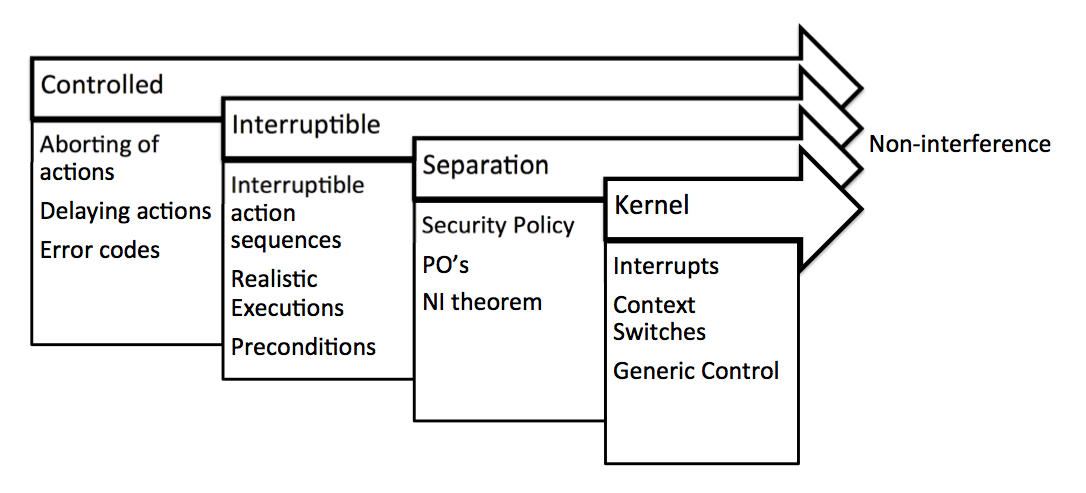
\includegraphics[width=\linewidth]{locales.png}
\caption{Overview of CISK modular structure}
\label{fig:extensions}
\end{figure}
% TODO


The second module adds a notion of separation, yielding a module of a Separation 
Kernel (SK). A security policy is added that dictates which domains may flow 
information to each other. Local proof obligations are added from which a global 
theorem of noninterference is proven. This global theorem is the \emph{unwinding} 
of the local proof obligations.
%The addition of a control mechanism to the model means that the traditional 
%formulation of intransitive noninterference no longer applies, as will be 
%explained in Section~\ref{sec:related}.
%We have reformulated noninterference to deal with control.

In the third module calls to the kernel are no longer considered atomic, 
yielding an Interruptible Separation Kernel (ISK).
In this model, one call to the kernel is represented by an \emph{action sequence}.
Consider, for example, an IPC call (for: Inter Process Communication). From the 
point of view of the programmer this is one kernel call. From the point of view 
of the kernel it is an action sequence consisting of three stages 
IPC\_PREP, IPC\_WAIT, and IPC\_SEND. 
During the PREP stage, it is checked whether the IPC is allowed by the security 
policy.
The WAIT stage is entered if a thread needs to wait for its communication partner.
The SEND stage is data transmission.
After each stage, an interrupt may occur that switches the current context.
A consequence of allowing interruptible action sequences is that it is no longer 
the case that any execution, i.e., any combination of atomic kernel actions, is 
realistic. We formulate a definition of \emph{realistic execution} and weaken 
the proof obligations of the model to apply only to realistic executions.

The final module provides an interpretation of control that allows atomic kernel 
actions to be aborted or delayed.
Additional proof obligations are required to ensure that noninterference is still 
provided.
This yields a Controlled Interruptible Separation Kernel (CISK).
When sequences of kernel actions are aborted, error codes can be transmitted to 
other domains.
Revisiting our IPC example, after the PREP stage the kernel can decide to abort 
the action. The IPC action sequence will not be continued and error codes may be 
sent out.
At the WAIT stage, the kernel can delay the action sequence until the communication 
partner of the IPC call is ready to receive.



% OLD
In Section~\ref{sect:generic} we introduce a theory of intransitive 
non-interference for separation kernels with control, based on~\cite{Verbeek2013}. 
We show that it can be instantiated for a simple API consisting of IPC and 
events (Section~\ref{sect:instantiation}). The rest of {\em this} section gives 
some auxiliary theories used for Section~\ref{sect:generic}.

\section{Preliminaries}

% generated text of all theories
\input{ListExtras.tex}

%
\begin{isabellebody}%
\def\isabellecontext{Secrecy{\isacharunderscore}types}%
%
\isamarkupheader{Auxiliary data types%
}
\isamarkuptrue%
%
\isadelimtheory
%
\endisadelimtheory
%
\isatagtheory
\isacommand{theory}\isamarkupfalse%
\ Secrecy{\isacharunderscore}types\isanewline
\isakeyword{imports}\ Main\isanewline
\isakeyword{begin}\isanewline
\isanewline
%
\isamarkupcmt{We assume disjoint sets: Data of data values,%
}
\isanewline
%
\isamarkupcmt{Secrets of unguessable values, Keys - set of cryptographic  keys.%
}
\ \ \isanewline
%
\isamarkupcmt{Based on these sets, we specify the sets EncType of encryptors that may be%
}
\isanewline
%
\isamarkupcmt{used for encryption or decryption, and Expression of expression items.%
}
\isanewline
%
\isamarkupcmt{The specification (component) identifiers should be listed in the set specID,%
}
\isanewline
%
\isamarkupcmt{the channel indentifiers should be listed in the set chanID.%
}
%
\endisatagtheory
{\isafoldtheory}%
%
\isadelimtheory
%
\endisadelimtheory
\ \isanewline
\isanewline
\isacommand{datatype}\isamarkupfalse%
\ Keys\ {\isacharequal}\ CKey\ {\isacharbar}\ CKeyP\ {\isacharbar}\ SKey\ {\isacharbar}\ SKeyP\ {\isacharbar}\ genKey\ \isanewline
\isacommand{datatype}\isamarkupfalse%
\ Secrets\ {\isacharequal}\ secretD\ {\isacharbar}\ N\ {\isacharbar}\ NA\isanewline
\isacommand{type{\isacharunderscore}synonym}\isamarkupfalse%
\ Var\ \ {\isacharequal}\ {\isachardoublequoteopen}nat{\isachardoublequoteclose}\isanewline
\isacommand{type{\isacharunderscore}synonym}\isamarkupfalse%
\ Data\ {\isacharequal}\ {\isachardoublequoteopen}nat{\isachardoublequoteclose}\isanewline
\isacommand{datatype}\isamarkupfalse%
\ KS\ \ \ \ \ \ \ \ \ \ {\isacharequal}\ kKS\ Keys\ {\isacharbar}\ sKS\ Secrets\isanewline
\isacommand{datatype}\isamarkupfalse%
\ EncType\ \ {\isacharequal}\ kEnc\ Keys\ {\isacharbar}\ vEnc\ Var\isanewline
\isacommand{datatype}\isamarkupfalse%
\ specID\ {\isacharequal}\ sComp{\isadigit{1}}\ {\isacharbar}\ sComp{\isadigit{2}}\ {\isacharbar}\ sComp{\isadigit{3}}\ {\isacharbar}\ sComp{\isadigit{4}}\isanewline
\isacommand{datatype}\isamarkupfalse%
\ Expression\ {\isacharequal}\ kE\ Keys\ {\isacharbar}\ sE\ Secrets\ {\isacharbar}\ dE\ Data\ {\isacharbar}\ idE\ specID\ \isanewline
\isacommand{datatype}\isamarkupfalse%
\ chanID\ {\isacharequal}\ ch{\isadigit{1}}\ {\isacharbar}\ ch{\isadigit{2}}\ \ \ {\isacharbar}\ ch{\isadigit{3}}\ \ {\isacharbar}\ ch{\isadigit{4}}\isanewline
\isanewline
\isacommand{primrec}\isamarkupfalse%
\ Expression{\isadigit{2}}KSL{\isacharcolon}{\isacharcolon}\ {\isachardoublequoteopen}Expression\ list\ {\isasymRightarrow}\ KS\ list{\isachardoublequoteclose}\ \isanewline
\isakeyword{where}\isanewline
\ \ \ {\isachardoublequoteopen}Expression{\isadigit{2}}KSL\ {\isacharbrackleft}{\isacharbrackright}\ {\isacharequal}\ {\isacharbrackleft}{\isacharbrackright}{\isachardoublequoteclose}\ {\isacharbar}\isanewline
\ \ \ {\isachardoublequoteopen}Expression{\isadigit{2}}KSL\ {\isacharparenleft}x{\isacharhash}xs{\isacharparenright}\ {\isacharequal}\ \isanewline
\ \ \ \ \ {\isacharparenleft}{\isacharparenleft}case\ x\ of\ {\isacharparenleft}kE\ m{\isacharparenright}\ {\isasymRightarrow}\ {\isacharbrackleft}kKS\ m{\isacharbrackright}\ \isanewline
\ \ \ \ \ \ \ \ \ \ \ \ \ \ \ \ \ \ {\isacharbar}\ {\isacharparenleft}sE\ m{\isacharparenright}\ {\isasymRightarrow}\ {\isacharbrackleft}sKS\ m{\isacharbrackright}\ \isanewline
\ \ \ \ \ \ \ \ \ \ \ \ \ \ \ \ \ \ {\isacharbar}\ {\isacharparenleft}dE\ m{\isacharparenright}\ {\isasymRightarrow}\ {\isacharbrackleft}{\isacharbrackright}\ \isanewline
\ \ \ \ \ \ \ \ \ \ \ \ \ \ \ \ \ \ {\isacharbar}\ {\isacharparenleft}idE\ m{\isacharparenright}\ {\isasymRightarrow}\ {\isacharbrackleft}{\isacharbrackright}{\isacharparenright}\ {\isacharat}\ Expression{\isadigit{2}}KSL\ xs{\isacharparenright}\ {\isachardoublequoteclose}\isanewline
\isanewline
\isacommand{primrec}\isamarkupfalse%
\ KS{\isadigit{2}}Expression{\isacharcolon}{\isacharcolon}\ {\isachardoublequoteopen}KS\ {\isasymRightarrow}\ Expression{\isachardoublequoteclose}\ \isanewline
\isakeyword{where}\isanewline
\ \ {\isachardoublequoteopen}KS{\isadigit{2}}Expression\ {\isacharparenleft}kKS\ m{\isacharparenright}\ {\isacharequal}\ {\isacharparenleft}kE\ m{\isacharparenright}{\isachardoublequoteclose}\ \ {\isacharbar}\isanewline
\ \ {\isachardoublequoteopen}KS{\isadigit{2}}Expression\ {\isacharparenleft}sKS\ m{\isacharparenright}\ {\isacharequal}\ {\isacharparenleft}sE\ m{\isacharparenright}{\isachardoublequoteclose}\isanewline
%
\isadelimtheory
\isanewline
%
\endisadelimtheory
%
\isatagtheory
\isacommand{end}\isamarkupfalse%
%
\endisatagtheory
{\isafoldtheory}%
%
\isadelimtheory
%
\endisadelimtheory
\end{isabellebody}%
%%% Local Variables:
%%% mode: latex
%%% TeX-master: "root"
%%% End:


%
\begin{isabellebody}%
\def\isabellecontext{inout}%
%
\isamarkupheader{Correctness of the relations between sets of Input/Output channels%
}
\isamarkuptrue%
%
\isadelimtheory
%
\endisadelimtheory
%
\isatagtheory
\isacommand{theory}\isamarkupfalse%
\ \ inout\ \isanewline
\isakeyword{imports}\ Secrecy{\isacharunderscore}types\isanewline
\isakeyword{begin}%
\endisatagtheory
{\isafoldtheory}%
%
\isadelimtheory
%
\endisadelimtheory
\isanewline
\isanewline
\isacommand{consts}\isamarkupfalse%
\ \isanewline
\ \ subcomponents\ {\isacharcolon}{\isacharcolon}\ \ {\isachardoublequoteopen}specID\ {\isasymRightarrow}\ specID\ set{\isachardoublequoteclose}\isanewline
\isanewline
%
\isamarkupcmt{Mappings, defining sets of input, local, and output channels%
}
\isanewline
%
\isamarkupcmt{of a component%
}
\isanewline
\isacommand{consts}\isamarkupfalse%
\isanewline
\ \ ins\ {\isacharcolon}{\isacharcolon}\ {\isachardoublequoteopen}specID\ {\isasymRightarrow}\ chanID\ set{\isachardoublequoteclose}\isanewline
\ \ loc\ {\isacharcolon}{\isacharcolon}\ {\isachardoublequoteopen}specID\ {\isasymRightarrow}\ chanID\ set{\isachardoublequoteclose}\isanewline
\ \ out\ {\isacharcolon}{\isacharcolon}\ {\isachardoublequoteopen}specID\ {\isasymRightarrow}\ chanID\ set{\isachardoublequoteclose}\isanewline
\isanewline
%
\isamarkupcmt{Predicate insuring the correct mapping from the component identifier%
}
\isanewline
%
\isamarkupcmt{to the set of input channels of a component%
}
\isanewline
\isacommand{definition}\isamarkupfalse%
\isanewline
\ \ inStream\ {\isacharcolon}{\isacharcolon}\ {\isachardoublequoteopen}specID\ {\isasymRightarrow}\ chanID\ set\ {\isasymRightarrow}\ bool{\isachardoublequoteclose}\isanewline
\isakeyword{where}\isanewline
\ \ {\isachardoublequoteopen}inStream\ x\ y\ \ {\isasymequiv}\ {\isacharparenleft}ins\ x\ {\isacharequal}\ y{\isacharparenright}{\isachardoublequoteclose}\isanewline
\isanewline
%
\isamarkupcmt{Predicate insuring the correct mapping from the component identifier%
}
\isanewline
%
\isamarkupcmt{to the set of local channels of a component%
}
\isanewline
\isacommand{definition}\isamarkupfalse%
\isanewline
\ \ locStream\ {\isacharcolon}{\isacharcolon}\ {\isachardoublequoteopen}specID\ {\isasymRightarrow}\ chanID\ set\ {\isasymRightarrow}\ bool{\isachardoublequoteclose}\isanewline
\isakeyword{where}\isanewline
\ \ {\isachardoublequoteopen}locStream\ x\ y\ {\isasymequiv}\ {\isacharparenleft}loc\ x\ {\isacharequal}\ y{\isacharparenright}{\isachardoublequoteclose}\isanewline
\isanewline
%
\isamarkupcmt{Predicate insuring the correct mapping from the component identifier%
}
\isanewline
%
\isamarkupcmt{to the set of output channels of a component%
}
\isanewline
\isacommand{definition}\isamarkupfalse%
\isanewline
\ \ outStream\ {\isacharcolon}{\isacharcolon}\ {\isachardoublequoteopen}specID\ {\isasymRightarrow}\ chanID\ set\ {\isasymRightarrow}\ bool{\isachardoublequoteclose}\isanewline
\isakeyword{where}\isanewline
\ \ {\isachardoublequoteopen}outStream\ x\ y\ {\isasymequiv}\ {\isacharparenleft}out\ x\ {\isacharequal}\ y{\isacharparenright}{\isachardoublequoteclose}\isanewline
\isanewline
%
\isamarkupcmt{Predicate insuring the correct relations between%
}
\isanewline
%
\isamarkupcmt{to the set of input, output and local channels of a component%
}
\isanewline
\isacommand{definition}\isamarkupfalse%
\isanewline
\ \ correctInOutLoc\ {\isacharcolon}{\isacharcolon}\ {\isachardoublequoteopen}specID\ {\isasymRightarrow}\ bool{\isachardoublequoteclose}\isanewline
\isakeyword{where}\isanewline
\ \ {\isachardoublequoteopen}correctInOutLoc\ x\ {\isasymequiv}\ \isanewline
\ \ \ {\isacharparenleft}ins\ x{\isacharparenright}\ {\isasyminter}\ {\isacharparenleft}out\ x{\isacharparenright}\ {\isacharequal}\ {\isacharbraceleft}{\isacharbraceright}\ \isanewline
\ \ \ \ {\isasymand}\ {\isacharparenleft}ins\ x{\isacharparenright}\ {\isasyminter}\ {\isacharparenleft}loc\ x{\isacharparenright}\ {\isacharequal}\ {\isacharbraceleft}{\isacharbraceright}\ \isanewline
\ \ \ \ {\isasymand}\ {\isacharparenleft}loc\ x{\isacharparenright}\ {\isasyminter}\ {\isacharparenleft}out\ x{\isacharparenright}\ {\isacharequal}\ {\isacharbraceleft}{\isacharbraceright}\ {\isachardoublequoteclose}\ \isanewline
\isanewline
%
\isamarkupcmt{Predicate insuring the correct relations between%
}
\isanewline
%
\isamarkupcmt{sets of input channels within a composed component%
}
\isanewline
\isacommand{definition}\isamarkupfalse%
\isanewline
\ \ correctCompositionIn\ {\isacharcolon}{\isacharcolon}\ {\isachardoublequoteopen}specID\ {\isasymRightarrow}\ bool{\isachardoublequoteclose}\isanewline
\isakeyword{where}\isanewline
\ \ {\isachardoublequoteopen}correctCompositionIn\ x\ {\isasymequiv}\ \isanewline
\ \ {\isacharparenleft}ins\ x{\isacharparenright}\ {\isacharequal}\ {\isacharparenleft}{\isasymUnion}\ {\isacharparenleft}ins\ {\isacharbackquote}\ {\isacharparenleft}subcomponents\ x{\isacharparenright}{\isacharparenright}\ {\isacharminus}\ {\isacharparenleft}loc\ x{\isacharparenright}{\isacharparenright}\isanewline
\ \ {\isasymand}\ {\isacharparenleft}ins\ x{\isacharparenright}\ {\isasyminter}\ {\isacharparenleft}{\isasymUnion}\ {\isacharparenleft}out\ {\isacharbackquote}\ {\isacharparenleft}subcomponents\ x{\isacharparenright}{\isacharparenright}{\isacharparenright}\ {\isacharequal}\ {\isacharbraceleft}{\isacharbraceright}{\isachardoublequoteclose}\ \isanewline
\isanewline
%
\isamarkupcmt{Predicate insuring the correct relations between%
}
\isanewline
%
\isamarkupcmt{sets of output channels within a composed component%
}
\isanewline
\isacommand{definition}\isamarkupfalse%
\isanewline
\ \ correctCompositionOut\ {\isacharcolon}{\isacharcolon}\ {\isachardoublequoteopen}specID\ {\isasymRightarrow}\ bool{\isachardoublequoteclose}\isanewline
\isakeyword{where}\isanewline
\ \ {\isachardoublequoteopen}correctCompositionOut\ x\ {\isasymequiv}\ \isanewline
\ \ {\isacharparenleft}out\ x{\isacharparenright}\ {\isacharequal}\ {\isacharparenleft}{\isasymUnion}\ {\isacharparenleft}out\ {\isacharbackquote}\ {\isacharparenleft}subcomponents\ x{\isacharparenright}{\isacharparenright}{\isacharminus}\ {\isacharparenleft}loc\ x{\isacharparenright}{\isacharparenright}\isanewline
\ \ {\isasymand}\ {\isacharparenleft}out\ x{\isacharparenright}\ {\isasyminter}\ {\isacharparenleft}{\isasymUnion}\ {\isacharparenleft}ins\ {\isacharbackquote}\ {\isacharparenleft}subcomponents\ x{\isacharparenright}{\isacharparenright}{\isacharparenright}\ {\isacharequal}\ {\isacharbraceleft}{\isacharbraceright}\ {\isachardoublequoteclose}\ \isanewline
\isanewline
%
\isamarkupcmt{Predicate insuring the correct relations between%
}
\isanewline
%
\isamarkupcmt{sets of local channels within a composed component%
}
\isanewline
\isacommand{definition}\isamarkupfalse%
\isanewline
\ \ correctCompositionLoc\ {\isacharcolon}{\isacharcolon}\ {\isachardoublequoteopen}specID\ {\isasymRightarrow}\ bool{\isachardoublequoteclose}\isanewline
\isakeyword{where}\isanewline
\ \ {\isachardoublequoteopen}correctCompositionLoc\ x\ {\isasymequiv}\ \isanewline
\ \ \ {\isacharparenleft}loc\ x{\isacharparenright}\ {\isacharequal}\ {\isasymUnion}\ {\isacharparenleft}ins\ {\isacharbackquote}\ {\isacharparenleft}subcomponents\ x{\isacharparenright}{\isacharparenright}\isanewline
\ \ \ \ \ \ \ \ \ \ \ {\isasyminter}\ {\isasymUnion}\ {\isacharparenleft}out\ {\isacharbackquote}\ {\isacharparenleft}subcomponents\ x{\isacharparenright}{\isacharparenright}{\isachardoublequoteclose}\ \isanewline
\isanewline
%
\isamarkupcmt{If a component is an elementary one (has no subcomponents)%
}
\isanewline
%
\isamarkupcmt{its set of local channels should be empty%
}
\isanewline
\isacommand{lemma}\isamarkupfalse%
\ subcomponents{\isacharunderscore}loc{\isacharcolon}\isanewline
\isakeyword{assumes}\ {\isachardoublequoteopen}correctCompositionLoc\ x{\isachardoublequoteclose}\isanewline
\ \ \ \ \ \ \ \isakeyword{and}\ {\isachardoublequoteopen}subcomponents\ x\ {\isacharequal}\ {\isacharbraceleft}{\isacharbraceright}{\isachardoublequoteclose}\isanewline
\isakeyword{shows}\ {\isachardoublequoteopen}loc\ x\ {\isacharequal}\ {\isacharbraceleft}{\isacharbraceright}{\isachardoublequoteclose}\isanewline
%
\isadelimproof
%
\endisadelimproof
%
\isatagproof
\isacommand{using}\isamarkupfalse%
\ assms\ \isacommand{by}\isamarkupfalse%
\ {\isacharparenleft}simp\ add{\isacharcolon}\ correctCompositionLoc{\isacharunderscore}def{\isacharparenright}%
\endisatagproof
{\isafoldproof}%
%
\isadelimproof
\isanewline
%
\endisadelimproof
%
\isadelimtheory
\isanewline
%
\endisadelimtheory
%
\isatagtheory
\isacommand{end}\isamarkupfalse%
%
\endisatagtheory
{\isafoldtheory}%
%
\isadelimtheory
%
\endisadelimtheory
\end{isabellebody}%
%%% Local Variables:
%%% mode: latex
%%% TeX-master: "root"
%%% End:


%
\begin{isabellebody}%
\def\isabellecontext{Secrecy}%
%
\isamarkupheader{Secrecy: Definitions and properties%
}
\isamarkuptrue%
%
\isadelimtheory
%
\endisadelimtheory
%
\isatagtheory
\isacommand{theory}\isamarkupfalse%
\ Secrecy\isanewline
\isakeyword{imports}\ Secrecy{\isacharunderscore}types\ inout\ ListExtras\isanewline
\isakeyword{begin}\isanewline
\isanewline
%
\isamarkupcmt{Encryption, decryption, signature creation and signature verification functions%
}
\isanewline
%
\isamarkupcmt{For these functions we define only their signatures and general axioms,%
}
\isanewline
%
\isamarkupcmt{because in order to reason effectively, we view them as abstract functions and%
}
\isanewline
%
\isamarkupcmt{abstract from their implementation details%
}
%
\endisatagtheory
{\isafoldtheory}%
%
\isadelimtheory
%
\endisadelimtheory
\ \isanewline
\isacommand{consts}\isamarkupfalse%
\ \isanewline
\ \ Enc\ \ {\isacharcolon}{\isacharcolon}\ {\isachardoublequoteopen}Keys\ {\isasymRightarrow}\ Expression\ list\ {\isasymRightarrow}\ Expression\ list{\isachardoublequoteclose}\isanewline
\ \ Decr\ {\isacharcolon}{\isacharcolon}\ {\isachardoublequoteopen}Keys\ {\isasymRightarrow}\ Expression\ list\ {\isasymRightarrow}\ Expression\ list{\isachardoublequoteclose}\isanewline
\ \ Sign\ {\isacharcolon}{\isacharcolon}\ {\isachardoublequoteopen}Keys\ {\isasymRightarrow}\ Expression\ list\ {\isasymRightarrow}\ Expression\ list{\isachardoublequoteclose}\isanewline
\ \ Ext\ \ \ {\isacharcolon}{\isacharcolon}\ {\isachardoublequoteopen}Keys\ {\isasymRightarrow}\ Expression\ list\ {\isasymRightarrow}\ Expression\ list{\isachardoublequoteclose}\isanewline
\isanewline
%
\isamarkupcmt{Axioms on relations between encription and decription keys%
}
\isanewline
\isacommand{axiomatization}\isamarkupfalse%
\isanewline
\ \ \ EncrDecrKeys\ {\isacharcolon}{\isacharcolon}\ {\isachardoublequoteopen}Keys\ \ {\isasymRightarrow}\ Keys\ {\isasymRightarrow}\ bool{\isachardoublequoteclose}\isanewline
\isakeyword{where}\isanewline
ExtSign{\isacharcolon}\ \isanewline
\ {\isachardoublequoteopen}EncrDecrKeys\ K{\isadigit{1}}\ K{\isadigit{2}}\ {\isasymlongrightarrow}\ {\isacharparenleft}Ext\ K{\isadigit{1}}\ {\isacharparenleft}Sign\ K{\isadigit{2}}\ E{\isacharparenright}{\isacharparenright}\ {\isacharequal}\ E{\isachardoublequoteclose}\ \ \isakeyword{and}\isanewline
DecrEnc{\isacharcolon}\isanewline
\ {\isachardoublequoteopen}EncrDecrKeys\ K{\isadigit{1}}\ K{\isadigit{2}}\ {\isasymlongrightarrow}\ {\isacharparenleft}Decr\ K{\isadigit{2}}\ {\isacharparenleft}Enc\ K{\isadigit{1}}\ E{\isacharparenright}{\isacharparenright}\ {\isacharequal}\ E{\isachardoublequoteclose}\isanewline
\isanewline
%
\isamarkupcmt{Set of private keys of a component%
}
\isanewline
\isacommand{consts}\isamarkupfalse%
\isanewline
\ specKeys\ {\isacharcolon}{\isacharcolon}\ {\isachardoublequoteopen}specID\ {\isasymRightarrow}\ Keys\ set{\isachardoublequoteclose}\isanewline
%
\isamarkupcmt{Set of unguessable values used by a component%
}
\isanewline
\isacommand{consts}\isamarkupfalse%
\ \isanewline
\ specSecrets\ {\isacharcolon}{\isacharcolon}\ {\isachardoublequoteopen}specID\ {\isasymRightarrow}\ Secrets\ set{\isachardoublequoteclose}\isanewline
\isanewline
%
\isamarkupcmt{Join set of private keys and unguessable values used by a component%
}
\isanewline
\isacommand{definition}\isamarkupfalse%
\isanewline
\ \ specKeysSecrets\ {\isacharcolon}{\isacharcolon}\ {\isachardoublequoteopen}specID\ {\isasymRightarrow}\ KS\ set{\isachardoublequoteclose}\isanewline
\isakeyword{where}\isanewline
\ {\isachardoublequoteopen}specKeysSecrets\ C\ {\isasymequiv}\isanewline
\ \ {\isacharbraceleft}y\ {\isachardot}\ \ {\isasymexists}\ x{\isachardot}\ y\ {\isacharequal}\ {\isacharparenleft}kKS\ x{\isacharparenright}\ \ {\isasymand}\ {\isacharparenleft}x\ {\isasymin}\ {\isacharparenleft}specKeys\ C{\isacharparenright}{\isacharparenright}{\isacharbraceright}\ {\isasymunion}\isanewline
\ \ {\isacharbraceleft}z\ {\isachardot}\ \ {\isasymexists}\ s{\isachardot}\ z\ {\isacharequal}\ {\isacharparenleft}sKS\ s{\isacharparenright}\ \ {\isasymand}\ {\isacharparenleft}s\ {\isasymin}\ {\isacharparenleft}specSecrets\ C{\isacharparenright}{\isacharparenright}{\isacharbraceright}{\isachardoublequoteclose}\isanewline
\isanewline
%
\isamarkupcmt{Predicate defining that a list of expression items does not contain%
}
\isanewline
%
\isamarkupcmt{any private key  or unguessable value used by a component%
}
\isanewline
\isacommand{definition}\isamarkupfalse%
\isanewline
\ \ notSpecKeysSecretsExpr\ {\isacharcolon}{\isacharcolon}\ {\isachardoublequoteopen}specID\ {\isasymRightarrow}\ \ Expression\ list\ {\isasymRightarrow}\ bool{\isachardoublequoteclose}\isanewline
\isakeyword{where}\isanewline
\ \ \ \ \ {\isachardoublequoteopen}notSpecKeysSecretsExpr\ P\ e\ {\isasymequiv}\isanewline
\ \ \ \ \ {\isacharparenleft}{\isasymforall}\ x{\isachardot}\ {\isacharparenleft}kE\ x{\isacharparenright}\ mem\ e\ {\isasymlongrightarrow}\ {\isacharparenleft}kKS\ x{\isacharparenright}\ {\isasymnotin}\ specKeysSecrets\ P{\isacharparenright}\ {\isasymand}\isanewline
\ \ \ \ \ {\isacharparenleft}{\isasymforall}\ y{\isachardot}\ {\isacharparenleft}sE\ y{\isacharparenright}\ mem\ e\ {\isasymlongrightarrow}\ {\isacharparenleft}sKS\ y{\isacharparenright}\ {\isasymnotin}\ specKeysSecrets\ P{\isacharparenright}{\isachardoublequoteclose}\isanewline
\isanewline
%
\isamarkupcmt{If a component is a composite one, the set of its private keys%
}
\ \isanewline
%
\isamarkupcmt{is a union of the subcomponents' sets of the private keys%
}
\isanewline
\isacommand{definition}\isamarkupfalse%
\isanewline
\ \ correctCompositionKeys\ {\isacharcolon}{\isacharcolon}\ \ {\isachardoublequoteopen}specID\ {\isasymRightarrow}\ bool{\isachardoublequoteclose}\isanewline
\isakeyword{where}\isanewline
\ \ {\isachardoublequoteopen}correctCompositionKeys\ x\ {\isasymequiv}\isanewline
\ \ \ \ subcomponents\ x\ {\isasymnoteq}\ {\isacharbraceleft}{\isacharbraceright}\ {\isasymlongrightarrow}\ \isanewline
\ \ \ \ specKeys\ x\ {\isacharequal}\ \ {\isasymUnion}\ {\isacharparenleft}specKeys\ {\isacharbackquote}\ {\isacharparenleft}subcomponents\ x{\isacharparenright}{\isacharparenright}{\isachardoublequoteclose}\ \isanewline
\isanewline
%
\isamarkupcmt{If a component is a composite one, the set of its unguessable values%
}
\ \isanewline
%
\isamarkupcmt{is a union of the subcomponents' sets of the unguessable values%
}
\isanewline
\isacommand{definition}\isamarkupfalse%
\isanewline
\ \ correctCompositionSecrets\ {\isacharcolon}{\isacharcolon}\ \ {\isachardoublequoteopen}specID\ {\isasymRightarrow}\ bool{\isachardoublequoteclose}\isanewline
\isakeyword{where}\isanewline
\ \ {\isachardoublequoteopen}correctCompositionSecrets\ x\ {\isasymequiv}\isanewline
\ \ \ \ subcomponents\ x\ {\isasymnoteq}\ {\isacharbraceleft}{\isacharbraceright}\ {\isasymlongrightarrow}\ \isanewline
\ \ \ \ specSecrets\ x\ {\isacharequal}\ \ {\isasymUnion}\ {\isacharparenleft}specSecrets\ {\isacharbackquote}\ {\isacharparenleft}subcomponents\ x{\isacharparenright}{\isacharparenright}{\isachardoublequoteclose}\ \isanewline
\isanewline
%
\isamarkupcmt{If a component is a composite one, the set of its private keys and%
}
\ \isanewline
%
\isamarkupcmt{unguessable values is a union of the corresponding sets of its subcomponents%
}
\isanewline
\isacommand{definition}\isamarkupfalse%
\isanewline
\ \ correctCompositionKS\ {\isacharcolon}{\isacharcolon}\ \ {\isachardoublequoteopen}specID\ {\isasymRightarrow}\ bool{\isachardoublequoteclose}\isanewline
\isakeyword{where}\isanewline
\ \ {\isachardoublequoteopen}correctCompositionKS\ x\ {\isasymequiv}\isanewline
\ \ \ \ subcomponents\ x\ {\isasymnoteq}\ {\isacharbraceleft}{\isacharbraceright}\ {\isasymlongrightarrow}\ \isanewline
\ \ \ \ specKeysSecrets\ x\ {\isacharequal}\ \ {\isasymUnion}\ {\isacharparenleft}specKeysSecrets\ {\isacharbackquote}\ {\isacharparenleft}subcomponents\ x{\isacharparenright}{\isacharparenright}{\isachardoublequoteclose}\ \isanewline
\isanewline
%
\isamarkupcmt{Predicate defining set of correctness properties of the component's%
}
\isanewline
%
\isamarkupcmt{interface  and relations on its private keys and unguessable values%
}
\isanewline
\isacommand{definition}\isamarkupfalse%
\isanewline
\ \ correctComponentSecrecy\ \ {\isacharcolon}{\isacharcolon}\ \ {\isachardoublequoteopen}specID\ {\isasymRightarrow}\ bool{\isachardoublequoteclose}\isanewline
\isakeyword{where}\ \isanewline
\ \ {\isachardoublequoteopen}correctComponentSecrecy\ x\ {\isasymequiv}\ \isanewline
\ \ \ \ correctCompositionKS\ x\ {\isasymand}\ \isanewline
\ \ \ \ correctCompositionSecrets\ x\ {\isasymand}\ \isanewline
\ \ \ \ correctCompositionKeys\ x\ {\isasymand}\ \isanewline
\ \ \ \ correctCompositionLoc\ x\ {\isasymand}\isanewline
\ \ \ \ correctCompositionIn\ x\ {\isasymand}\isanewline
\ \ \ \ correctCompositionOut\ x\ {\isasymand}\ \isanewline
\ \ \ \ correctInOutLoc\ x{\isachardoublequoteclose}\isanewline
\isanewline
%
\isamarkupcmt{Predicate exprChannel I E defines whether the expression item E can be sent via the channel I%
}
\ \ \ \ \isanewline
\isacommand{consts}\isamarkupfalse%
\isanewline
\ exprChannel\ {\isacharcolon}{\isacharcolon}\ {\isachardoublequoteopen}chanID\ {\isasymRightarrow}\ Expression\ {\isasymRightarrow}\ bool{\isachardoublequoteclose}\isanewline
\isanewline
%
\isamarkupcmt{Predicate eoutM sP M E defines whether the component sP may eventually%
}
\isanewline
%
\isamarkupcmt{output an expression E if there exists a time interval t of%
}
\ \isanewline
%
\isamarkupcmt{an output channel which contains this expression E%
}
\isanewline
\isacommand{definition}\isamarkupfalse%
\isanewline
\ \ eout\ {\isacharcolon}{\isacharcolon}\ {\isachardoublequoteopen}specID\ \ {\isasymRightarrow}\ Expression\ {\isasymRightarrow}\ bool{\isachardoublequoteclose}\isanewline
\isakeyword{where}\isanewline
\ {\isachardoublequoteopen}eout\ sP\ E\ {\isasymequiv}\ \isanewline
\ \ {\isasymexists}\ {\isacharparenleft}ch\ {\isacharcolon}{\isacharcolon}\ chanID{\isacharparenright}{\isachardot}\ {\isacharparenleft}{\isacharparenleft}ch\ {\isasymin}\ {\isacharparenleft}out\ sP{\isacharparenright}{\isacharparenright}\ {\isasymand}\ {\isacharparenleft}exprChannel\ ch\ E{\isacharparenright}{\isacharparenright}{\isachardoublequoteclose}\isanewline
\isanewline
%
\isamarkupcmt{Predicate eout sP E defines whether the component sP may eventually%
}
\isanewline
%
\isamarkupcmt{output an expression E via subset of channels M,%
}
\isanewline
%
\isamarkupcmt{which is a subset of output channels of sP,%
}
\isanewline
%
\isamarkupcmt{and if there exists a time interval t of%
}
\ \isanewline
%
\isamarkupcmt{an output channel which contains this expression E%
}
\isanewline
\isacommand{definition}\isamarkupfalse%
\isanewline
\ \ eoutM\ {\isacharcolon}{\isacharcolon}\ {\isachardoublequoteopen}specID\ \ {\isasymRightarrow}\ chanID\ set\ {\isasymRightarrow}\ Expression\ {\isasymRightarrow}\ bool{\isachardoublequoteclose}\isanewline
\isakeyword{where}\isanewline
\ {\isachardoublequoteopen}eoutM\ sP\ M\ E\ {\isasymequiv}\ \isanewline
\ \ {\isasymexists}\ {\isacharparenleft}ch\ {\isacharcolon}{\isacharcolon}\ chanID{\isacharparenright}{\isachardot}\ {\isacharparenleft}{\isacharparenleft}ch\ {\isasymin}\ {\isacharparenleft}out\ sP{\isacharparenright}{\isacharparenright}\ {\isasymand}\ {\isacharparenleft}ch\ {\isasymin}\ M{\isacharparenright}\ {\isasymand}\ {\isacharparenleft}exprChannel\ ch\ E{\isacharparenright}{\isacharparenright}{\isachardoublequoteclose}\isanewline
\isanewline
%
\isamarkupcmt{Predicate ineM sP M E defines whether a component sP may eventually%
}
\isanewline
%
\isamarkupcmt{get an expression E  if there exists a time interval t of%
}
\ \isanewline
%
\isamarkupcmt{an input stream  which contains this expression E%
}
\isanewline
\isacommand{definition}\isamarkupfalse%
\isanewline
\ \ ine\ {\isacharcolon}{\isacharcolon}\ {\isachardoublequoteopen}specID\ \ {\isasymRightarrow}\ Expression\ {\isasymRightarrow}\ bool{\isachardoublequoteclose}\isanewline
\isakeyword{where}\isanewline
\ {\isachardoublequoteopen}ine\ sP\ E\ {\isasymequiv}\ \isanewline
\ \ {\isasymexists}\ {\isacharparenleft}ch\ {\isacharcolon}{\isacharcolon}\ chanID{\isacharparenright}{\isachardot}\ {\isacharparenleft}{\isacharparenleft}ch\ {\isasymin}\ {\isacharparenleft}ins\ sP{\isacharparenright}{\isacharparenright}\ {\isasymand}\ {\isacharparenleft}exprChannel\ ch\ E{\isacharparenright}{\isacharparenright}{\isachardoublequoteclose}\isanewline
\isanewline
%
\isamarkupcmt{Predicate ine sP E defines whether a component sP may eventually%
}
\isanewline
%
\isamarkupcmt{get an expression E via subset of channels M,%
}
\isanewline
%
\isamarkupcmt{which is a subset of input channels of sP,%
}
\isanewline
%
\isamarkupcmt{and if there exists a time interval t of%
}
\ \isanewline
%
\isamarkupcmt{an input stream  which contains this expression E%
}
\isanewline
\isacommand{definition}\isamarkupfalse%
\isanewline
\ \ ineM\ {\isacharcolon}{\isacharcolon}\ {\isachardoublequoteopen}specID\ \ {\isasymRightarrow}\ chanID\ set\ {\isasymRightarrow}\ Expression\ {\isasymRightarrow}\ bool{\isachardoublequoteclose}\isanewline
\isakeyword{where}\isanewline
\ {\isachardoublequoteopen}ineM\ sP\ M\ E\ {\isasymequiv}\ \isanewline
\ \ {\isasymexists}\ {\isacharparenleft}ch\ {\isacharcolon}{\isacharcolon}\ chanID{\isacharparenright}{\isachardot}\ {\isacharparenleft}{\isacharparenleft}ch\ {\isasymin}\ {\isacharparenleft}ins\ sP{\isacharparenright}{\isacharparenright}\ {\isasymand}\ {\isacharparenleft}ch\ {\isasymin}\ M{\isacharparenright}\ {\isasymand}\ {\isacharparenleft}exprChannel\ ch\ E{\isacharparenright}{\isacharparenright}{\isachardoublequoteclose}\isanewline
\isanewline
%
\isamarkupcmt{This predicate defines whether an input channel ch of a component sP%
}
\isanewline
%
\isamarkupcmt{is the only one input channel of this component%
}
\isanewline
%
\isamarkupcmt{via which it may eventually output an expression E%
}
\isanewline
\isacommand{definition}\isamarkupfalse%
\isanewline
\ \ out{\isacharunderscore}exprChannelSingle\ {\isacharcolon}{\isacharcolon}\ {\isachardoublequoteopen}specID\ \ {\isasymRightarrow}\ chanID\ {\isasymRightarrow}\ Expression\ {\isasymRightarrow}\ bool{\isachardoublequoteclose}\isanewline
\isakeyword{where}\isanewline
\ {\isachardoublequoteopen}out{\isacharunderscore}exprChannelSingle\ sP\ ch\ E\ {\isasymequiv}\ \isanewline
\ \ {\isacharparenleft}ch\ {\isasymin}\ {\isacharparenleft}out\ sP{\isacharparenright}{\isacharparenright}\ {\isasymand}\ \ \isanewline
\ \ {\isacharparenleft}exprChannel\ ch\ E{\isacharparenright}\ \ {\isasymand}\isanewline
\ \ {\isacharparenleft}{\isasymforall}\ {\isacharparenleft}x\ {\isacharcolon}{\isacharcolon}\ chanID{\isacharparenright}\ {\isacharparenleft}t\ {\isacharcolon}{\isacharcolon}\ nat{\isacharparenright}{\isachardot}\ {\isacharparenleft}{\isacharparenleft}x\ {\isasymin}\ {\isacharparenleft}out\ sP{\isacharparenright}{\isacharparenright}\ {\isasymand}\ {\isacharparenleft}x\ {\isasymnoteq}\ ch{\isacharparenright}\ {\isasymlongrightarrow}\ {\isasymnot}\ exprChannel\ x\ E{\isacharparenright}{\isacharparenright}{\isachardoublequoteclose}\isanewline
\isanewline
%
\isamarkupcmt{This predicate  yields true if only the channels from the set chSet,%
}
\isanewline
%
\isamarkupcmt{which is a subset of input channels of the  component sP,%
}
\isanewline
%
\isamarkupcmt{may eventually output an expression E%
}
\isanewline
\isacommand{definition}\isamarkupfalse%
\isanewline
\ out{\isacharunderscore}exprChannelSet\ {\isacharcolon}{\isacharcolon}\ {\isachardoublequoteopen}specID\ \ {\isasymRightarrow}\ chanID\ set\ {\isasymRightarrow}\ Expression\ {\isasymRightarrow}\ bool{\isachardoublequoteclose}\isanewline
\isakeyword{where}\isanewline
\ {\isachardoublequoteopen}out{\isacharunderscore}exprChannelSet\ sP\ chSet\ E\ {\isasymequiv}\ \isanewline
\ \ \ {\isacharparenleft}{\isacharparenleft}{\isasymforall}\ {\isacharparenleft}x\ {\isacharcolon}{\isacharcolon}chanID{\isacharparenright}{\isachardot}\ {\isacharparenleft}{\isacharparenleft}x\ {\isasymin}\ chSet{\isacharparenright}\ {\isasymlongrightarrow}\ {\isacharparenleft}{\isacharparenleft}x\ {\isasymin}\ {\isacharparenleft}out\ sP{\isacharparenright}{\isacharparenright}\ {\isasymand}\ {\isacharparenleft}exprChannel\ x\ E{\isacharparenright}{\isacharparenright}{\isacharparenright}{\isacharparenright}\isanewline
\ \ \ {\isasymand}\isanewline
\ \ \ {\isacharparenleft}{\isasymforall}\ {\isacharparenleft}x\ {\isacharcolon}{\isacharcolon}\ chanID{\isacharparenright}{\isachardot}\ {\isacharparenleft}{\isacharparenleft}x\ {\isasymnotin}\ chSet{\isacharparenright}\ {\isasymand}\ {\isacharparenleft}x\ {\isasymin}\ {\isacharparenleft}out\ sP{\isacharparenright}{\isacharparenright}\ {\isasymlongrightarrow}\ {\isasymnot}\ exprChannel\ x\ E{\isacharparenright}{\isacharparenright}{\isacharparenright}{\isachardoublequoteclose}\isanewline
\isanewline
%
\isamarkupcmt{This redicate defines whether%
}
\isanewline
%
\isamarkupcmt{an input channel ch of a component sP is the only one input channel%
}
\isanewline
%
\isamarkupcmt{of this component via which it may eventually get an expression E%
}
\isanewline
\isacommand{definition}\isamarkupfalse%
\isanewline
\ ine{\isacharunderscore}exprChannelSingle\ {\isacharcolon}{\isacharcolon}\ {\isachardoublequoteopen}specID\ \ {\isasymRightarrow}\ chanID\ {\isasymRightarrow}\ Expression\ {\isasymRightarrow}\ bool{\isachardoublequoteclose}\isanewline
\isakeyword{where}\isanewline
\ {\isachardoublequoteopen}ine{\isacharunderscore}exprChannelSingle\ sP\ ch\ E\ {\isasymequiv}\ \isanewline
\ \ {\isacharparenleft}ch\ {\isasymin}\ {\isacharparenleft}ins\ sP{\isacharparenright}{\isacharparenright}\ {\isasymand}\isanewline
\ \ {\isacharparenleft}exprChannel\ ch\ E{\isacharparenright}\ \ {\isasymand}\isanewline
\ \ {\isacharparenleft}{\isasymforall}\ {\isacharparenleft}x\ {\isacharcolon}{\isacharcolon}\ chanID{\isacharparenright}\ {\isacharparenleft}t\ {\isacharcolon}{\isacharcolon}\ nat{\isacharparenright}{\isachardot}\ {\isacharparenleft}{\isacharparenleft}\ x\ {\isasymin}\ {\isacharparenleft}ins\ sP{\isacharparenright}{\isacharparenright}\ {\isasymand}\ {\isacharparenleft}x\ {\isasymnoteq}\ ch{\isacharparenright}\ {\isasymlongrightarrow}\ {\isasymnot}\ exprChannel\ x\ E{\isacharparenright}{\isacharparenright}{\isachardoublequoteclose}\isanewline
\isanewline
%
\isamarkupcmt{This predicate yields true if the component sP may eventually%
}
\isanewline
%
\isamarkupcmt{get an expression E only via the channels from the set chSet,%
}
\isanewline
%
\isamarkupcmt{which is a subset of input channels of sP%
}
\isanewline
\isacommand{definition}\isamarkupfalse%
\isanewline
\ ine{\isacharunderscore}exprChannelSet\ {\isacharcolon}{\isacharcolon}\ {\isachardoublequoteopen}specID\ \ {\isasymRightarrow}\ chanID\ set\ {\isasymRightarrow}\ Expression\ {\isasymRightarrow}\ bool{\isachardoublequoteclose}\isanewline
\isakeyword{where}\isanewline
\ {\isachardoublequoteopen}ine{\isacharunderscore}exprChannelSet\ sP\ chSet\ E\ {\isasymequiv}\ \isanewline
\ \ \ {\isacharparenleft}{\isacharparenleft}{\isasymforall}\ {\isacharparenleft}x\ {\isacharcolon}{\isacharcolon}chanID{\isacharparenright}{\isachardot}\ {\isacharparenleft}{\isacharparenleft}x\ {\isasymin}\ chSet{\isacharparenright}\ {\isasymlongrightarrow}\ {\isacharparenleft}{\isacharparenleft}x\ {\isasymin}\ {\isacharparenleft}ins\ sP{\isacharparenright}{\isacharparenright}\ {\isasymand}\ {\isacharparenleft}exprChannel\ x\ E{\isacharparenright}{\isacharparenright}{\isacharparenright}{\isacharparenright}\isanewline
\ \ \ {\isasymand}\isanewline
\ \ \ {\isacharparenleft}{\isasymforall}\ {\isacharparenleft}x\ {\isacharcolon}{\isacharcolon}\ chanID{\isacharparenright}{\isachardot}\ {\isacharparenleft}{\isacharparenleft}x\ {\isasymnotin}\ chSet{\isacharparenright}\ {\isasymand}\ {\isacharparenleft}\ x\ {\isasymin}\ {\isacharparenleft}ins\ sP{\isacharparenright}{\isacharparenright}\ {\isasymlongrightarrow}\ {\isasymnot}\ exprChannel\ x\ E{\isacharparenright}{\isacharparenright}{\isacharparenright}{\isachardoublequoteclose}\isanewline
\isanewline
%
\isamarkupcmt{If a list of expression items does not contain any private key%
}
\isanewline
%
\isamarkupcmt{or unguessable value of a component P, then the first element%
}
\ \isanewline
%
\isamarkupcmt{of the list is neither a private key nor unguessable value of P%
}
\isanewline
\isacommand{lemma}\isamarkupfalse%
\ notSpecKeysSecretsExpr{\isacharunderscore}L{\isadigit{1}}{\isacharcolon}\isanewline
\isakeyword{assumes}\ {\isachardoublequoteopen}notSpecKeysSecretsExpr\ P\ {\isacharparenleft}a\ {\isacharhash}\ l{\isacharparenright}{\isachardoublequoteclose}\isanewline
\isakeyword{shows}\ \ \ \ {\isachardoublequoteopen}notSpecKeysSecretsExpr\ P\ {\isacharbrackleft}a{\isacharbrackright}{\isachardoublequoteclose}\isanewline
%
\isadelimproof
%
\endisadelimproof
%
\isatagproof
\isacommand{using}\isamarkupfalse%
\ assms\ \isacommand{by}\isamarkupfalse%
\ {\isacharparenleft}simp\ add{\isacharcolon}\ notSpecKeysSecretsExpr{\isacharunderscore}def{\isacharparenright}\isanewline
\isanewline
%
\isamarkupcmt{If a list of expression items does not contain any private key%
}
\isanewline
%
\isamarkupcmt{or unguessable value of a component P, then this list without its first%
}
\ \isanewline
%
\isamarkupcmt{element does not contain them too%
}
%
\endisatagproof
{\isafoldproof}%
%
\isadelimproof
\isanewline
%
\endisadelimproof
\isacommand{lemma}\isamarkupfalse%
\ notSpecKeysSecretsExpr{\isacharunderscore}L{\isadigit{2}}{\isacharcolon}\isanewline
\isakeyword{assumes}\ {\isachardoublequoteopen}notSpecKeysSecretsExpr\ P\ {\isacharparenleft}a\ {\isacharhash}\ l{\isacharparenright}{\isachardoublequoteclose}\isanewline
\isakeyword{shows}\ \ \ \ {\isachardoublequoteopen}notSpecKeysSecretsExpr\ P\ l{\isachardoublequoteclose}\ \isanewline
%
\isadelimproof
%
\endisadelimproof
%
\isatagproof
\isacommand{using}\isamarkupfalse%
\ assms\ \isacommand{by}\isamarkupfalse%
\ {\isacharparenleft}simp\ add{\isacharcolon}\ notSpecKeysSecretsExpr{\isacharunderscore}def{\isacharparenright}\isanewline
\isanewline
%
\isamarkupcmt{If a channel belongs to the set of input channels of a component P%
}
\isanewline
%
\isamarkupcmt{and does not belong to the set of local channels of the compositon of P and Q%
}
\ \isanewline
%
\isamarkupcmt{then it belongs to the set of input channels of this composition%
}
%
\endisatagproof
{\isafoldproof}%
%
\isadelimproof
\isanewline
%
\endisadelimproof
\isacommand{lemma}\isamarkupfalse%
\ correctCompositionIn{\isacharunderscore}L{\isadigit{1}}{\isacharcolon}\isanewline
\isakeyword{assumes}\ {\isachardoublequoteopen}subcomponents\ PQ\ {\isacharequal}\ {\isacharbraceleft}P{\isacharcomma}Q{\isacharbraceright}{\isachardoublequoteclose}\ \isanewline
\ \ \ \ \ \ \ \isakeyword{and}\ {\isachardoublequoteopen}correctCompositionIn\ PQ{\isachardoublequoteclose}\ \isanewline
\ \ \ \ \ \ \ \isakeyword{and}\ {\isachardoublequoteopen}ch\ {\isasymnotin}\ loc\ PQ{\isachardoublequoteclose}\isanewline
\ \ \ \ \ \ \ \isakeyword{and}\ {\isachardoublequoteopen}ch\ {\isasymin}\ ins\ P{\isachardoublequoteclose}\ \isanewline
\isakeyword{shows}\ \ \ \ {\isachardoublequoteopen}ch\ {\isasymin}\ ins\ PQ{\isachardoublequoteclose}\isanewline
%
\isadelimproof
%
\endisadelimproof
%
\isatagproof
\isacommand{using}\isamarkupfalse%
\ assms\ \isacommand{by}\isamarkupfalse%
\ {\isacharparenleft}simp\ add{\isacharcolon}\ correctCompositionIn{\isacharunderscore}def{\isacharparenright}\isanewline
\isanewline
%
\isamarkupcmt{If a channel belongs to the set of input channels of the compositon of P and Q%
}
\isanewline
%
\isamarkupcmt{then it belongs to the set of input channels either of P or of Q%
}
%
\endisatagproof
{\isafoldproof}%
%
\isadelimproof
\isanewline
%
\endisadelimproof
\isacommand{lemma}\isamarkupfalse%
\ correctCompositionIn{\isacharunderscore}L{\isadigit{2}}{\isacharcolon}\isanewline
\isakeyword{assumes}\ {\isachardoublequoteopen}subcomponents\ PQ\ {\isacharequal}\ {\isacharbraceleft}P{\isacharcomma}Q{\isacharbraceright}{\isachardoublequoteclose}\isanewline
\ \ \ \ \ \ \ \isakeyword{and}\ {\isachardoublequoteopen}correctCompositionIn\ PQ{\isachardoublequoteclose}\ \isanewline
\ \ \ \ \ \ \ \isakeyword{and}\ {\isachardoublequoteopen}ch\ {\isasymin}\ ins\ PQ{\isachardoublequoteclose}\ \isanewline
\isakeyword{shows}\ \ \ \ {\isachardoublequoteopen}{\isacharparenleft}ch\ {\isasymin}\ ins\ P{\isacharparenright}\ {\isasymor}\ {\isacharparenleft}ch\ {\isasymin}\ ins\ Q{\isacharparenright}{\isachardoublequoteclose}\ \isanewline
%
\isadelimproof
%
\endisadelimproof
%
\isatagproof
\isacommand{using}\isamarkupfalse%
\ assms\ \isacommand{by}\isamarkupfalse%
\ {\isacharparenleft}simp\ add{\isacharcolon}\ correctCompositionIn{\isacharunderscore}def{\isacharparenright}%
\endisatagproof
{\isafoldproof}%
%
\isadelimproof
\isanewline
%
\endisadelimproof
\isanewline
\isacommand{lemma}\isamarkupfalse%
\ ineM{\isacharunderscore}L{\isadigit{1}}{\isacharcolon}\isanewline
\isakeyword{assumes}\ {\isachardoublequoteopen}ch\ {\isasymin}\ M{\isachardoublequoteclose}\ \isanewline
\ \ \ \ \ \ \ \isakeyword{and}\ {\isachardoublequoteopen}ch\ {\isasymin}\ ins\ P{\isachardoublequoteclose}\isanewline
\ \ \ \ \ \ \ \isakeyword{and}\ {\isachardoublequoteopen}exprChannel\ ch\ E{\isachardoublequoteclose}\isanewline
\isakeyword{shows}\ \ \ \ {\isachardoublequoteopen}ineM\ P\ M\ E{\isachardoublequoteclose}\isanewline
%
\isadelimproof
%
\endisadelimproof
%
\isatagproof
\isacommand{using}\isamarkupfalse%
\ assms\ \isacommand{by}\isamarkupfalse%
\ {\isacharparenleft}simp\ add{\isacharcolon}\ ineM{\isacharunderscore}def{\isacharcomma}\ blast{\isacharparenright}%
\endisatagproof
{\isafoldproof}%
%
\isadelimproof
\isanewline
%
\endisadelimproof
\isanewline
\isacommand{lemma}\isamarkupfalse%
\ ineM{\isacharunderscore}ine{\isacharcolon}\isanewline
\isakeyword{assumes}\ {\isachardoublequoteopen}ineM\ P\ M\ E{\isachardoublequoteclose}\isanewline
\isakeyword{shows}\ \ \ \ {\isachardoublequoteopen}ine\ P\ E{\isachardoublequoteclose}\isanewline
%
\isadelimproof
%
\endisadelimproof
%
\isatagproof
\isacommand{using}\isamarkupfalse%
\ assms\ \isacommand{by}\isamarkupfalse%
\ {\isacharparenleft}simp\ add{\isacharcolon}\ ineM{\isacharunderscore}def\ ine{\isacharunderscore}def{\isacharcomma}\ blast{\isacharparenright}%
\endisatagproof
{\isafoldproof}%
%
\isadelimproof
\isanewline
%
\endisadelimproof
\isanewline
\isacommand{lemma}\isamarkupfalse%
\ not{\isacharunderscore}ine{\isacharunderscore}ineM{\isacharcolon}\isanewline
\isakeyword{assumes}\ {\isachardoublequoteopen}{\isasymnot}\ ine\ P\ E{\isachardoublequoteclose}\isanewline
\isakeyword{shows}\ \ \ \ {\isachardoublequoteopen}{\isasymnot}\ ineM\ P\ M\ E{\isachardoublequoteclose}\isanewline
%
\isadelimproof
%
\endisadelimproof
%
\isatagproof
\isacommand{using}\isamarkupfalse%
\ assms\ \isacommand{by}\isamarkupfalse%
\ {\isacharparenleft}simp\ add{\isacharcolon}\ ineM{\isacharunderscore}def\ ine{\isacharunderscore}def{\isacharparenright}%
\endisatagproof
{\isafoldproof}%
%
\isadelimproof
\isanewline
%
\endisadelimproof
\isanewline
\isacommand{lemma}\isamarkupfalse%
\ eoutM{\isacharunderscore}eout{\isacharcolon}\isanewline
\isakeyword{assumes}\ {\isachardoublequoteopen}eoutM\ P\ M\ E{\isachardoublequoteclose}\isanewline
\isakeyword{shows}\ \ \ \ {\isachardoublequoteopen}eout\ P\ E{\isachardoublequoteclose}\isanewline
%
\isadelimproof
%
\endisadelimproof
%
\isatagproof
\isacommand{using}\isamarkupfalse%
\ assms\ \isacommand{by}\isamarkupfalse%
\ {\isacharparenleft}simp\ add{\isacharcolon}\ eoutM{\isacharunderscore}def\ eout{\isacharunderscore}def{\isacharcomma}\ blast{\isacharparenright}%
\endisatagproof
{\isafoldproof}%
%
\isadelimproof
\isanewline
%
\endisadelimproof
\isanewline
\isacommand{lemma}\isamarkupfalse%
\ not{\isacharunderscore}eout{\isacharunderscore}eoutM{\isacharcolon}\isanewline
\isakeyword{assumes}\ {\isachardoublequoteopen}{\isasymnot}\ eout\ P\ E{\isachardoublequoteclose}\isanewline
\isakeyword{shows}\ \ \ \ {\isachardoublequoteopen}{\isasymnot}\ eoutM\ P\ M\ E{\isachardoublequoteclose}\isanewline
%
\isadelimproof
%
\endisadelimproof
%
\isatagproof
\isacommand{using}\isamarkupfalse%
\ assms\ \isacommand{by}\isamarkupfalse%
\ {\isacharparenleft}simp\ add{\isacharcolon}\ eoutM{\isacharunderscore}def\ eout{\isacharunderscore}def{\isacharparenright}%
\endisatagproof
{\isafoldproof}%
%
\isadelimproof
\isanewline
%
\endisadelimproof
\isanewline
\isacommand{lemma}\isamarkupfalse%
\ correctCompositionKeys{\isacharunderscore}subcomp{\isadigit{1}}{\isacharcolon}\isanewline
\isakeyword{assumes}\ {\isachardoublequoteopen}correctCompositionKeys\ C{\isachardoublequoteclose}\isanewline
\ \ \ \ \ \ \ \ \isakeyword{and}\ {\isachardoublequoteopen}x\ {\isasymin}\ subcomponents\ C{\isachardoublequoteclose}\ \isanewline
\ \ \ \ \ \ \ \ \isakeyword{and}\ {\isachardoublequoteopen}xb\ {\isasymin}\ specKeys\ C{\isachardoublequoteclose}\isanewline
\isakeyword{shows}\ \ \ \ \ {\isachardoublequoteopen}{\isasymexists}\ x\ {\isasymin}\ subcomponents\ C{\isachardot}\ {\isacharparenleft}xb\ {\isasymin}\ specKeys\ x{\isacharparenright}{\isachardoublequoteclose}\isanewline
%
\isadelimproof
%
\endisadelimproof
%
\isatagproof
\isacommand{using}\isamarkupfalse%
\ assms\ \isacommand{by}\isamarkupfalse%
\ {\isacharparenleft}simp\ add{\isacharcolon}\ correctCompositionKeys{\isacharunderscore}def{\isacharcomma}\ auto{\isacharparenright}%
\endisatagproof
{\isafoldproof}%
%
\isadelimproof
\isanewline
%
\endisadelimproof
\isanewline
\isacommand{lemma}\isamarkupfalse%
\ correctCompositionSecrets{\isacharunderscore}subcomp{\isadigit{1}}{\isacharcolon}\isanewline
\isakeyword{assumes}\ {\isachardoublequoteopen}correctCompositionSecrets\ C{\isachardoublequoteclose}\ \isanewline
\ \ \ \ \ \ \ \ \isakeyword{and}\ {\isachardoublequoteopen}x\ {\isasymin}\ subcomponents\ C{\isachardoublequoteclose}\isanewline
\ \ \ \ \ \ \ \ \isakeyword{and}\ {\isachardoublequoteopen}s\ {\isasymin}\ specSecrets\ C{\isachardoublequoteclose}\isanewline
\isakeyword{shows}\ \ \ \ \ {\isachardoublequoteopen}{\isasymexists}\ x\ {\isasymin}\ subcomponents\ C{\isachardot}\ {\isacharparenleft}s\ {\isasymin}\ specSecrets\ x{\isacharparenright}{\isachardoublequoteclose}\isanewline
%
\isadelimproof
%
\endisadelimproof
%
\isatagproof
\isacommand{using}\isamarkupfalse%
\ assms\ \isacommand{by}\isamarkupfalse%
\ {\isacharparenleft}simp\ add{\isacharcolon}\ correctCompositionSecrets{\isacharunderscore}def{\isacharcomma}\ auto{\isacharparenright}%
\endisatagproof
{\isafoldproof}%
%
\isadelimproof
\isanewline
%
\endisadelimproof
\isanewline
\isacommand{lemma}\isamarkupfalse%
\ correctCompositionKeys{\isacharunderscore}subcomp{\isadigit{2}}{\isacharcolon}\isanewline
\isakeyword{assumes}\ {\isachardoublequoteopen}correctCompositionKeys\ C{\isachardoublequoteclose}\isanewline
\ \ \ \ \ \ \ \isakeyword{and}\ {\isachardoublequoteopen}xb\ {\isasymin}\ subcomponents\ C{\isachardoublequoteclose}\isanewline
\ \ \ \ \ \ \ \isakeyword{and}\ {\isachardoublequoteopen}xc\ {\isasymin}\ specKeys\ xb{\isachardoublequoteclose}\isanewline
\isakeyword{shows}\ \ \ \ {\isachardoublequoteopen}xc\ {\isasymin}\ specKeys\ C{\isachardoublequoteclose}\isanewline
%
\isadelimproof
%
\endisadelimproof
%
\isatagproof
\isacommand{using}\isamarkupfalse%
\ assms\ \isacommand{by}\isamarkupfalse%
\ {\isacharparenleft}simp\ add{\isacharcolon}\ correctCompositionKeys{\isacharunderscore}def{\isacharcomma}\ auto{\isacharparenright}%
\endisatagproof
{\isafoldproof}%
%
\isadelimproof
\isanewline
%
\endisadelimproof
\isanewline
\isacommand{lemma}\isamarkupfalse%
\ correctCompositionSecrets{\isacharunderscore}subcomp{\isadigit{2}}{\isacharcolon}\isanewline
\isakeyword{assumes}\ {\isachardoublequoteopen}correctCompositionSecrets\ C{\isachardoublequoteclose}\isanewline
\ \ \ \ \ \ \ \ \isakeyword{and}\ {\isachardoublequoteopen}xb\ {\isasymin}\ subcomponents\ C{\isachardoublequoteclose}\isanewline
\ \ \ \ \ \ \ \ \isakeyword{and}\ {\isachardoublequoteopen}xc\ {\isasymin}\ specSecrets\ xb{\isachardoublequoteclose}\isanewline
\isakeyword{shows}\ \ \ \ \ {\isachardoublequoteopen}xc\ {\isasymin}\ specSecrets\ C{\isachardoublequoteclose}\isanewline
%
\isadelimproof
%
\endisadelimproof
%
\isatagproof
\isacommand{using}\isamarkupfalse%
\ assms\ \isacommand{by}\isamarkupfalse%
\ {\isacharparenleft}simp\ add{\isacharcolon}\ correctCompositionSecrets{\isacharunderscore}def{\isacharcomma}\ auto{\isacharparenright}%
\endisatagproof
{\isafoldproof}%
%
\isadelimproof
\isanewline
%
\endisadelimproof
\isanewline
\isacommand{lemma}\isamarkupfalse%
\ correctCompKS{\isacharunderscore}Keys{\isacharcolon}\isanewline
\isakeyword{assumes}\ {\isachardoublequoteopen}correctCompositionKS\ C{\isachardoublequoteclose}\isanewline
\isakeyword{shows}\ \ \ \ {\isachardoublequoteopen}correctCompositionKeys\ C{\isachardoublequoteclose}\isanewline
%
\isadelimproof
%
\endisadelimproof
%
\isatagproof
\isacommand{proof}\isamarkupfalse%
\ {\isacharparenleft}cases\ {\isachardoublequoteopen}subcomponents\ C\ {\isacharequal}\ {\isacharbraceleft}{\isacharbraceright}{\isachardoublequoteclose}{\isacharparenright}\isanewline
\ \ \isacommand{assume}\isamarkupfalse%
\ {\isachardoublequoteopen}subcomponents\ C\ {\isacharequal}\ {\isacharbraceleft}{\isacharbraceright}{\isachardoublequoteclose}\isanewline
\ \ \isacommand{from}\isamarkupfalse%
\ this\ \isakeyword{and}\ assms\ \isacommand{show}\isamarkupfalse%
\ {\isacharquery}thesis\isanewline
\ \ \isacommand{by}\isamarkupfalse%
\ {\isacharparenleft}simp\ add{\isacharcolon}\ correctCompositionKeys{\isacharunderscore}def{\isacharparenright}\isanewline
\isacommand{next}\isamarkupfalse%
\isanewline
\ \ \isacommand{assume}\isamarkupfalse%
\ {\isachardoublequoteopen}subcomponents\ C\ {\isasymnoteq}\ {\isacharbraceleft}{\isacharbraceright}{\isachardoublequoteclose}\isanewline
\ \ \isacommand{from}\isamarkupfalse%
\ this\ \isakeyword{and}\ assms\ \isacommand{show}\isamarkupfalse%
\ {\isacharquery}thesis\ \isanewline
\ \ \isacommand{by}\isamarkupfalse%
\ {\isacharparenleft}simp\ add{\isacharcolon}\ correctCompositionKS{\isacharunderscore}def\ \isanewline
\ \ \ \ \ \ \ \ \ \ \ \ \ \ \ \ correctCompositionKeys{\isacharunderscore}def\isanewline
\ \ \ \ \ \ \ \ \ \ \ \ \ \ \ \ specKeysSecrets{\isacharunderscore}def{\isacharcomma}\ blast{\isacharparenright}\isanewline
\isacommand{qed}\isamarkupfalse%
%
\endisatagproof
{\isafoldproof}%
%
\isadelimproof
\isanewline
%
\endisadelimproof
\isanewline
\isacommand{lemma}\isamarkupfalse%
\ correctCompKS{\isacharunderscore}Secrets{\isacharcolon}\isanewline
\isakeyword{assumes}\ {\isachardoublequoteopen}correctCompositionKS\ C{\isachardoublequoteclose}\isanewline
\isakeyword{shows}\ \ \ \ {\isachardoublequoteopen}correctCompositionSecrets\ C{\isachardoublequoteclose}\isanewline
%
\isadelimproof
%
\endisadelimproof
%
\isatagproof
\isacommand{proof}\isamarkupfalse%
\ {\isacharparenleft}cases\ {\isachardoublequoteopen}subcomponents\ C\ {\isacharequal}\ {\isacharbraceleft}{\isacharbraceright}{\isachardoublequoteclose}{\isacharparenright}\isanewline
\ \ \isacommand{assume}\isamarkupfalse%
\ {\isachardoublequoteopen}subcomponents\ C\ {\isacharequal}\ {\isacharbraceleft}{\isacharbraceright}{\isachardoublequoteclose}\isanewline
\ \ \isacommand{from}\isamarkupfalse%
\ this\ \isakeyword{and}\ assms\ \isacommand{show}\isamarkupfalse%
\ {\isacharquery}thesis\isanewline
\ \ \isacommand{by}\isamarkupfalse%
\ {\isacharparenleft}simp\ add{\isacharcolon}\ correctCompositionSecrets{\isacharunderscore}def{\isacharparenright}\isanewline
\isacommand{next}\isamarkupfalse%
\isanewline
\ \ \isacommand{assume}\isamarkupfalse%
\ {\isachardoublequoteopen}subcomponents\ C\ {\isasymnoteq}\ {\isacharbraceleft}{\isacharbraceright}{\isachardoublequoteclose}\isanewline
\ \ \isacommand{from}\isamarkupfalse%
\ this\ \isakeyword{and}\ assms\ \isacommand{show}\isamarkupfalse%
\ {\isacharquery}thesis\ \isanewline
\ \ \isacommand{by}\isamarkupfalse%
\ {\isacharparenleft}simp\ add{\isacharcolon}\ correctCompositionKS{\isacharunderscore}def\ \isanewline
\ \ \ \ \ \ \ \ \ \ \ \ \ \ \ \ correctCompositionSecrets{\isacharunderscore}def\isanewline
\ \ \ \ \ \ \ \ \ \ \ \ \ \ \ \ specKeysSecrets{\isacharunderscore}def{\isacharcomma}\ blast{\isacharparenright}\isanewline
\isacommand{qed}\isamarkupfalse%
%
\endisatagproof
{\isafoldproof}%
%
\isadelimproof
\isanewline
%
\endisadelimproof
\isanewline
\isacommand{lemma}\isamarkupfalse%
\ correctCompKS{\isacharunderscore}KeysSecrets{\isacharcolon}\isanewline
\isakeyword{assumes}\ {\isachardoublequoteopen}correctCompositionKeys\ C{\isachardoublequoteclose}\isanewline
\ \ \ \ \ \ \ \ \isakeyword{and}\ {\isachardoublequoteopen}correctCompositionSecrets\ C{\isachardoublequoteclose}\isanewline
\isakeyword{shows}\ \ \ \ {\isachardoublequoteopen}correctCompositionKS\ C{\isachardoublequoteclose}\isanewline
%
\isadelimproof
%
\endisadelimproof
%
\isatagproof
\isacommand{proof}\isamarkupfalse%
\ {\isacharparenleft}cases\ {\isachardoublequoteopen}subcomponents\ C\ {\isacharequal}\ {\isacharbraceleft}{\isacharbraceright}{\isachardoublequoteclose}{\isacharparenright}\isanewline
\ \ \isacommand{assume}\isamarkupfalse%
\ {\isachardoublequoteopen}subcomponents\ C\ {\isacharequal}\ {\isacharbraceleft}{\isacharbraceright}{\isachardoublequoteclose}\isanewline
\ \ \isacommand{from}\isamarkupfalse%
\ this\ \isakeyword{and}\ assms\ \isacommand{show}\isamarkupfalse%
\ {\isacharquery}thesis\isanewline
\ \ \isacommand{by}\isamarkupfalse%
\ {\isacharparenleft}simp\ add{\isacharcolon}\ correctCompositionKS{\isacharunderscore}def{\isacharparenright}\isanewline
\isacommand{next}\isamarkupfalse%
\isanewline
\ \ \isacommand{assume}\isamarkupfalse%
\ {\isachardoublequoteopen}subcomponents\ C\ {\isasymnoteq}\ {\isacharbraceleft}{\isacharbraceright}{\isachardoublequoteclose}\isanewline
\ \ \isacommand{from}\isamarkupfalse%
\ this\ \isakeyword{and}\ assms\ \isacommand{show}\isamarkupfalse%
\ {\isacharquery}thesis\ \isanewline
\ \ \isacommand{by}\isamarkupfalse%
\ {\isacharparenleft}simp\ add{\isacharcolon}\ correctCompositionKS{\isacharunderscore}def\ \isanewline
\ \ \ \ \ \ \ \ \ \ \ \ \ \ \ \ correctCompositionKeys{\isacharunderscore}def\ \isanewline
\ \ \ \ \ \ \ \ \ \ \ \ \ \ \ \ correctCompositionSecrets{\isacharunderscore}def\isanewline
\ \ \ \ \ \ \ \ \ \ \ \ \ \ \ \ specKeysSecrets{\isacharunderscore}def{\isacharcomma}\ blast{\isacharparenright}\isanewline
\isacommand{qed}\isamarkupfalse%
%
\endisatagproof
{\isafoldproof}%
%
\isadelimproof
\ \isanewline
%
\endisadelimproof
\isanewline
\isacommand{lemma}\isamarkupfalse%
\ correctCompositionKS{\isacharunderscore}subcomp{\isadigit{1}}{\isacharcolon}\isanewline
\isakeyword{assumes}\ h{\isadigit{1}}{\isacharcolon}{\isachardoublequoteopen}correctCompositionKS\ C{\isachardoublequoteclose}\isanewline
\ \ \ \ \ \ \ \isakeyword{and}\ h{\isadigit{2}}{\isacharcolon}{\isachardoublequoteopen}x\ {\isasymin}\ subcomponents\ C{\isachardoublequoteclose}\isanewline
\ \ \ \ \ \ \ \isakeyword{and}\ h{\isadigit{3}}{\isacharcolon}{\isachardoublequoteopen}xa\ {\isasymin}\ specKeys\ C{\isachardoublequoteclose}\isanewline
\isakeyword{shows}\ \ \ \ {\isachardoublequoteopen}{\isasymexists}\ y\ {\isasymin}\ subcomponents\ C{\isachardot}\ {\isacharparenleft}xa\ {\isasymin}\ specKeys\ y{\isacharparenright}{\isachardoublequoteclose}\isanewline
%
\isadelimproof
%
\endisadelimproof
%
\isatagproof
\isacommand{proof}\isamarkupfalse%
\ {\isacharparenleft}cases\ {\isachardoublequoteopen}subcomponents\ C\ {\isacharequal}\ {\isacharbraceleft}{\isacharbraceright}{\isachardoublequoteclose}{\isacharparenright}\isanewline
\ \ \isacommand{assume}\isamarkupfalse%
\ {\isachardoublequoteopen}subcomponents\ C\ {\isacharequal}\ {\isacharbraceleft}{\isacharbraceright}{\isachardoublequoteclose}\isanewline
\ \ \isacommand{from}\isamarkupfalse%
\ this\ \isakeyword{and}\ h{\isadigit{2}}\ \isacommand{show}\isamarkupfalse%
\ {\isacharquery}thesis\ \isacommand{by}\isamarkupfalse%
\ simp\ \isanewline
\isacommand{next}\isamarkupfalse%
\isanewline
\ \ \isacommand{assume}\isamarkupfalse%
\ {\isachardoublequoteopen}subcomponents\ C\ {\isasymnoteq}\ {\isacharbraceleft}{\isacharbraceright}{\isachardoublequoteclose}\isanewline
\ \ \isacommand{from}\isamarkupfalse%
\ this\ \isakeyword{and}\ assms\ \isacommand{show}\isamarkupfalse%
\ {\isacharquery}thesis\ \isanewline
\ \ \isacommand{by}\isamarkupfalse%
\ {\isacharparenleft}simp\ add{\isacharcolon}\ correctCompositionKS{\isacharunderscore}def\ specKeysSecrets{\isacharunderscore}def{\isacharcomma}\ blast{\isacharparenright}\ \isanewline
\isacommand{qed}\isamarkupfalse%
%
\endisatagproof
{\isafoldproof}%
%
\isadelimproof
\isanewline
%
\endisadelimproof
\isanewline
\isacommand{lemma}\isamarkupfalse%
\ correctCompositionKS{\isacharunderscore}subcomp{\isadigit{2}}{\isacharcolon}\isanewline
\isakeyword{assumes}\ h{\isadigit{1}}{\isacharcolon}{\isachardoublequoteopen}correctCompositionKS\ C{\isachardoublequoteclose}\isanewline
\ \ \ \ \ \ \ \ \isakeyword{and}\ h{\isadigit{2}}{\isacharcolon}{\isachardoublequoteopen}x\ {\isasymin}\ subcomponents\ C{\isachardoublequoteclose}\isanewline
\ \ \ \ \ \ \ \ \isakeyword{and}\ h{\isadigit{3}}{\isacharcolon}{\isachardoublequoteopen}xa\ {\isasymin}\ specSecrets\ C{\isachardoublequoteclose}\isanewline
\isakeyword{shows}\ \ \ \ {\isachardoublequoteopen}{\isasymexists}\ y\ {\isasymin}\ subcomponents\ C{\isachardot}\ xa\ {\isasymin}\ specSecrets\ y{\isachardoublequoteclose}\isanewline
%
\isadelimproof
%
\endisadelimproof
%
\isatagproof
\isacommand{proof}\isamarkupfalse%
\ {\isacharparenleft}cases\ {\isachardoublequoteopen}subcomponents\ C\ {\isacharequal}\ {\isacharbraceleft}{\isacharbraceright}{\isachardoublequoteclose}{\isacharparenright}\isanewline
\ \ \isacommand{assume}\isamarkupfalse%
\ {\isachardoublequoteopen}subcomponents\ C\ {\isacharequal}\ {\isacharbraceleft}{\isacharbraceright}{\isachardoublequoteclose}\isanewline
\ \ \isacommand{from}\isamarkupfalse%
\ this\ \isakeyword{and}\ h{\isadigit{2}}\ \isacommand{show}\isamarkupfalse%
\ {\isacharquery}thesis\ \isacommand{by}\isamarkupfalse%
\ simp\ \isanewline
\isacommand{next}\isamarkupfalse%
\isanewline
\ \ \isacommand{assume}\isamarkupfalse%
\ {\isachardoublequoteopen}subcomponents\ C\ {\isasymnoteq}\ {\isacharbraceleft}{\isacharbraceright}{\isachardoublequoteclose}\isanewline
\ \ \isacommand{from}\isamarkupfalse%
\ this\ \isakeyword{and}\ assms\ \isacommand{show}\isamarkupfalse%
\ {\isacharquery}thesis\ \isanewline
\ \ \isacommand{by}\isamarkupfalse%
\ {\isacharparenleft}simp\ add{\isacharcolon}\ correctCompositionKS{\isacharunderscore}def\ specKeysSecrets{\isacharunderscore}def{\isacharcomma}\ blast{\isacharparenright}\isanewline
\isacommand{qed}\isamarkupfalse%
%
\endisatagproof
{\isafoldproof}%
%
\isadelimproof
\isanewline
%
\endisadelimproof
\isanewline
\isacommand{lemma}\isamarkupfalse%
\ correctCompositionKS{\isacharunderscore}subcomp{\isadigit{3}}{\isacharcolon}\isanewline
\isakeyword{assumes}\ {\isachardoublequoteopen}correctCompositionKS\ C{\isachardoublequoteclose}\isanewline
\ \ \ \ \ \ \ \isakeyword{and}\ {\isachardoublequoteopen}x\ {\isasymin}\ subcomponents\ C{\isachardoublequoteclose}\isanewline
\ \ \ \ \ \ \ \isakeyword{and}\ {\isachardoublequoteopen}xa\ {\isasymin}\ specKeys\ x{\isachardoublequoteclose}\isanewline
\isakeyword{shows}\ \ \ \ {\isachardoublequoteopen}xa\ {\isasymin}\ specKeys\ C{\isachardoublequoteclose}\isanewline
%
\isadelimproof
%
\endisadelimproof
%
\isatagproof
\isacommand{using}\isamarkupfalse%
\ assms\ \isanewline
\isacommand{by}\isamarkupfalse%
\ {\isacharparenleft}simp\ add{\isacharcolon}\ correctCompositionKS{\isacharunderscore}def\ specKeysSecrets{\isacharunderscore}def{\isacharcomma}\ auto{\isacharparenright}%
\endisatagproof
{\isafoldproof}%
%
\isadelimproof
\isanewline
%
\endisadelimproof
\isanewline
\isacommand{lemma}\isamarkupfalse%
\ correctCompositionKS{\isacharunderscore}subcomp{\isadigit{4}}{\isacharcolon}\isanewline
\isakeyword{assumes}\ {\isachardoublequoteopen}correctCompositionKS\ C{\isachardoublequoteclose}\isanewline
\ \ \ \ \ \ \ \ \isakeyword{and}\ {\isachardoublequoteopen}x\ {\isasymin}\ subcomponents\ C{\isachardoublequoteclose}\isanewline
\ \ \ \ \ \ \ \ \isakeyword{and}\ {\isachardoublequoteopen}xa\ {\isasymin}\ specSecrets\ x{\isachardoublequoteclose}\ \isanewline
\isakeyword{shows}\ \ \ \ \ {\isachardoublequoteopen}xa\ {\isasymin}\ specSecrets\ C{\isachardoublequoteclose}\isanewline
%
\isadelimproof
%
\endisadelimproof
%
\isatagproof
\isacommand{using}\isamarkupfalse%
\ assms\ \isanewline
\isacommand{by}\isamarkupfalse%
\ {\isacharparenleft}simp\ add{\isacharcolon}\ correctCompositionKS{\isacharunderscore}def\ specKeysSecrets{\isacharunderscore}def{\isacharcomma}\ auto{\isacharparenright}%
\endisatagproof
{\isafoldproof}%
%
\isadelimproof
\isanewline
%
\endisadelimproof
\isanewline
\isacommand{lemma}\isamarkupfalse%
\ correctCompositionKS{\isacharunderscore}PQ{\isacharcolon}\isanewline
\isakeyword{assumes}\ {\isachardoublequoteopen}subcomponents\ PQ\ {\isacharequal}\ {\isacharbraceleft}P{\isacharcomma}\ Q{\isacharbraceright}{\isachardoublequoteclose}\isanewline
\ \ \ \ \ \ \ \isakeyword{and}\ {\isachardoublequoteopen}correctCompositionKS\ PQ{\isachardoublequoteclose}\ \isanewline
\ \ \ \ \ \ \ \isakeyword{and}\ {\isachardoublequoteopen}ks\ {\isasymin}\ specKeysSecrets\ PQ{\isachardoublequoteclose}\isanewline
\isakeyword{shows}\ \ \ \ {\isachardoublequoteopen}ks\ {\isasymin}\ specKeysSecrets\ P\ {\isasymor}\ ks\ {\isasymin}\ specKeysSecrets\ Q{\isachardoublequoteclose}\isanewline
%
\isadelimproof
%
\endisadelimproof
%
\isatagproof
\isacommand{using}\isamarkupfalse%
\ assms\ \isacommand{by}\isamarkupfalse%
\ {\isacharparenleft}simp\ add{\isacharcolon}\ correctCompositionKS{\isacharunderscore}def{\isacharparenright}%
\endisatagproof
{\isafoldproof}%
%
\isadelimproof
\isanewline
%
\endisadelimproof
\isanewline
\isacommand{lemma}\isamarkupfalse%
\ correctCompositionKS{\isacharunderscore}neg{\isadigit{1}}{\isacharcolon}\isanewline
\isakeyword{assumes}\ {\isachardoublequoteopen}subcomponents\ PQ\ {\isacharequal}\ {\isacharbraceleft}P{\isacharcomma}\ Q{\isacharbraceright}{\isachardoublequoteclose}\isanewline
\ \ \ \ \ \ \ \isakeyword{and}\ {\isachardoublequoteopen}correctCompositionKS\ PQ{\isachardoublequoteclose}\ \isanewline
\ \ \ \ \ \ \ \isakeyword{and}\ {\isachardoublequoteopen}ks\ {\isasymnotin}\ specKeysSecrets\ P{\isachardoublequoteclose}\isanewline
\ \ \ \ \ \ \ \isakeyword{and}\ {\isachardoublequoteopen}ks\ {\isasymnotin}\ specKeysSecrets\ Q{\isachardoublequoteclose}\isanewline
\isakeyword{shows}\ \ \ \ {\isachardoublequoteopen}ks\ {\isasymnotin}\ specKeysSecrets\ PQ{\isachardoublequoteclose}\isanewline
%
\isadelimproof
%
\endisadelimproof
%
\isatagproof
\isacommand{using}\isamarkupfalse%
\ assms\ \isacommand{by}\isamarkupfalse%
\ {\isacharparenleft}simp\ add{\isacharcolon}\ correctCompositionKS{\isacharunderscore}def{\isacharparenright}%
\endisatagproof
{\isafoldproof}%
%
\isadelimproof
\isanewline
%
\endisadelimproof
\isanewline
\isacommand{lemma}\isamarkupfalse%
\ correctCompositionKS{\isacharunderscore}negP{\isacharcolon}\isanewline
\isakeyword{assumes}\ {\isachardoublequoteopen}subcomponents\ PQ\ {\isacharequal}\ {\isacharbraceleft}P{\isacharcomma}\ Q{\isacharbraceright}{\isachardoublequoteclose}\isanewline
\ \ \ \ \ \ \ \ \isakeyword{and}\ {\isachardoublequoteopen}correctCompositionKS\ PQ{\isachardoublequoteclose}\ \isanewline
\ \ \ \ \ \ \ \ \isakeyword{and}\ {\isachardoublequoteopen}ks\ {\isasymnotin}\ specKeysSecrets\ PQ{\isachardoublequoteclose}\ \isanewline
\isakeyword{shows}\ \ \ \ \ {\isachardoublequoteopen}ks\ {\isasymnotin}\ specKeysSecrets\ P{\isachardoublequoteclose}\isanewline
%
\isadelimproof
%
\endisadelimproof
%
\isatagproof
\isacommand{using}\isamarkupfalse%
\ assms\ \isacommand{by}\isamarkupfalse%
\ {\isacharparenleft}simp\ add{\isacharcolon}\ correctCompositionKS{\isacharunderscore}def{\isacharparenright}%
\endisatagproof
{\isafoldproof}%
%
\isadelimproof
\isanewline
%
\endisadelimproof
\isanewline
\isacommand{lemma}\isamarkupfalse%
\ correctCompositionKS{\isacharunderscore}negQ{\isacharcolon}\isanewline
\isakeyword{assumes}\ {\isachardoublequoteopen}subcomponents\ PQ\ {\isacharequal}\ {\isacharbraceleft}P{\isacharcomma}\ Q{\isacharbraceright}{\isachardoublequoteclose}\isanewline
\ \ \ \ \ \ \ \ \isakeyword{and}\ {\isachardoublequoteopen}correctCompositionKS\ PQ{\isachardoublequoteclose}\ \isanewline
\ \ \ \ \ \ \ \ \isakeyword{and}\ {\isachardoublequoteopen}ks\ {\isasymnotin}\ specKeysSecrets\ PQ{\isachardoublequoteclose}\ \isanewline
\isakeyword{shows}\ \ \ \ \ {\isachardoublequoteopen}ks\ {\isasymnotin}\ specKeysSecrets\ Q{\isachardoublequoteclose}\isanewline
%
\isadelimproof
%
\endisadelimproof
%
\isatagproof
\isacommand{using}\isamarkupfalse%
\ assms\ \isacommand{by}\isamarkupfalse%
\ {\isacharparenleft}simp\ add{\isacharcolon}\ correctCompositionKS{\isacharunderscore}def{\isacharparenright}%
\endisatagproof
{\isafoldproof}%
%
\isadelimproof
\isanewline
%
\endisadelimproof
\isanewline
\isacommand{lemma}\isamarkupfalse%
\ out{\isacharunderscore}exprChannelSingle{\isacharunderscore}Set{\isacharcolon}\isanewline
\isakeyword{assumes}\ {\isachardoublequoteopen}out{\isacharunderscore}exprChannelSingle\ P\ ch\ E{\isachardoublequoteclose}\isanewline
\isakeyword{shows}\ \ \ \ {\isachardoublequoteopen}out{\isacharunderscore}exprChannelSet\ P\ {\isacharbraceleft}ch{\isacharbraceright}\ E{\isachardoublequoteclose}\isanewline
%
\isadelimproof
%
\endisadelimproof
%
\isatagproof
\isacommand{using}\isamarkupfalse%
\ assms\ \isanewline
\isacommand{by}\isamarkupfalse%
\ {\isacharparenleft}simp\ add{\isacharcolon}\ out{\isacharunderscore}exprChannelSingle{\isacharunderscore}def\ out{\isacharunderscore}exprChannelSet{\isacharunderscore}def{\isacharparenright}%
\endisatagproof
{\isafoldproof}%
%
\isadelimproof
\isanewline
%
\endisadelimproof
\isanewline
\isacommand{lemma}\isamarkupfalse%
\ out{\isacharunderscore}exprChannelSet{\isacharunderscore}Single{\isacharcolon}\isanewline
\isakeyword{assumes}\ {\isachardoublequoteopen}out{\isacharunderscore}exprChannelSet\ P\ {\isacharbraceleft}ch{\isacharbraceright}\ E{\isachardoublequoteclose}\isanewline
\isakeyword{shows}\ \ \ \ {\isachardoublequoteopen}out{\isacharunderscore}exprChannelSingle\ P\ ch\ E{\isachardoublequoteclose}\isanewline
%
\isadelimproof
%
\endisadelimproof
%
\isatagproof
\isacommand{using}\isamarkupfalse%
\ assms\isanewline
\isacommand{by}\isamarkupfalse%
\ {\isacharparenleft}simp\ add{\isacharcolon}\ out{\isacharunderscore}exprChannelSingle{\isacharunderscore}def\ out{\isacharunderscore}exprChannelSet{\isacharunderscore}def{\isacharparenright}%
\endisatagproof
{\isafoldproof}%
%
\isadelimproof
\isanewline
%
\endisadelimproof
\isanewline
\isacommand{lemma}\isamarkupfalse%
\ ine{\isacharunderscore}exprChannelSingle{\isacharunderscore}Set{\isacharcolon}\isanewline
\isakeyword{assumes}\ {\isachardoublequoteopen}ine{\isacharunderscore}exprChannelSingle\ P\ ch\ E{\isachardoublequoteclose}\isanewline
\ \ \isakeyword{shows}\ {\isachardoublequoteopen}ine{\isacharunderscore}exprChannelSet\ P\ {\isacharbraceleft}ch{\isacharbraceright}\ E{\isachardoublequoteclose}\isanewline
%
\isadelimproof
%
\endisadelimproof
%
\isatagproof
\isacommand{using}\isamarkupfalse%
\ assms\ \isanewline
\isacommand{by}\isamarkupfalse%
\ {\isacharparenleft}simp\ add{\isacharcolon}\ ine{\isacharunderscore}exprChannelSingle{\isacharunderscore}def\ ine{\isacharunderscore}exprChannelSet{\isacharunderscore}def{\isacharparenright}%
\endisatagproof
{\isafoldproof}%
%
\isadelimproof
\isanewline
%
\endisadelimproof
\isanewline
\isacommand{lemma}\isamarkupfalse%
\ ine{\isacharunderscore}exprChannelSet{\isacharunderscore}Single{\isacharcolon}\isanewline
\isakeyword{assumes}\ {\isachardoublequoteopen}ine{\isacharunderscore}exprChannelSet\ P\ {\isacharbraceleft}ch{\isacharbraceright}\ E{\isachardoublequoteclose}\isanewline
\isakeyword{shows}\ \ \ \ {\isachardoublequoteopen}ine{\isacharunderscore}exprChannelSingle\ P\ ch\ E{\isachardoublequoteclose}\isanewline
%
\isadelimproof
%
\endisadelimproof
%
\isatagproof
\isacommand{using}\isamarkupfalse%
\ assms\ \isanewline
\isacommand{by}\isamarkupfalse%
\ {\isacharparenleft}simp\ add{\isacharcolon}\ ine{\isacharunderscore}exprChannelSingle{\isacharunderscore}def\ ine{\isacharunderscore}exprChannelSet{\isacharunderscore}def{\isacharparenright}%
\endisatagproof
{\isafoldproof}%
%
\isadelimproof
\isanewline
%
\endisadelimproof
\isanewline
\isacommand{lemma}\isamarkupfalse%
\ ine{\isacharunderscore}ins{\isacharunderscore}neg{\isadigit{1}}{\isacharcolon}\isanewline
\isakeyword{assumes}\ {\isachardoublequoteopen}{\isasymnot}\ ine\ P\ m{\isachardoublequoteclose}\ \isanewline
\ \ \ \ \ \ \ \isakeyword{and}\ {\isachardoublequoteopen}exprChannel\ x\ m{\isachardoublequoteclose}\isanewline
\isakeyword{shows}\ \ \ \ {\isachardoublequoteopen}x\ {\isasymnotin}\ ins\ P{\isachardoublequoteclose}\isanewline
%
\isadelimproof
%
\endisadelimproof
%
\isatagproof
\isacommand{using}\isamarkupfalse%
\ assms\ \isacommand{by}\isamarkupfalse%
\ {\isacharparenleft}simp\ add{\isacharcolon}\ ine{\isacharunderscore}def{\isacharcomma}\ auto{\isacharparenright}%
\endisatagproof
{\isafoldproof}%
%
\isadelimproof
\isanewline
%
\endisadelimproof
\isanewline
\isacommand{theorem}\isamarkupfalse%
\ TBtheorem{\isadigit{1}}a{\isacharcolon}\isanewline
\isakeyword{assumes}\ {\isachardoublequoteopen}ine\ PQ\ E{\isachardoublequoteclose}\ \isanewline
\ \ \ \ \ \ \ \isakeyword{and}\ {\isachardoublequoteopen}subcomponents\ PQ\ {\isacharequal}\ {\isacharbraceleft}P{\isacharcomma}Q{\isacharbraceright}{\isachardoublequoteclose}\isanewline
\ \ \ \ \ \ \ \isakeyword{and}\ {\isachardoublequoteopen}correctCompositionIn\ PQ{\isachardoublequoteclose}\isanewline
\isakeyword{shows}\ {\isachardoublequoteopen}ine\ P\ E\ \ {\isasymor}\ ine\ Q\ E{\isachardoublequoteclose}\isanewline
%
\isadelimproof
%
\endisadelimproof
%
\isatagproof
\isacommand{using}\isamarkupfalse%
\ assms\ \isacommand{by}\isamarkupfalse%
\ {\isacharparenleft}simp\ add{\isacharcolon}\ ine{\isacharunderscore}def\ correctCompositionIn{\isacharunderscore}def{\isacharcomma}\ auto{\isacharparenright}%
\endisatagproof
{\isafoldproof}%
%
\isadelimproof
\isanewline
%
\endisadelimproof
\isanewline
\isacommand{theorem}\isamarkupfalse%
\ TBtheorem{\isadigit{1}}b{\isacharcolon}\isanewline
\isakeyword{assumes}\ {\isachardoublequoteopen}ineM\ PQ\ M\ E{\isachardoublequoteclose}\isanewline
\ \ \ \ \ \ \ \isakeyword{and}\ {\isachardoublequoteopen}subcomponents\ PQ\ {\isacharequal}\ {\isacharbraceleft}P{\isacharcomma}Q{\isacharbraceright}{\isachardoublequoteclose}\isanewline
\ \ \ \ \ \ \ \isakeyword{and}\ {\isachardoublequoteopen}correctCompositionIn\ PQ{\isachardoublequoteclose}\ \isanewline
\isakeyword{shows}\ \ \ \ {\isachardoublequoteopen}ineM\ P\ M\ E\ {\isasymor}\ ineM\ Q\ M\ E{\isachardoublequoteclose}\isanewline
%
\isadelimproof
%
\endisadelimproof
%
\isatagproof
\isacommand{using}\isamarkupfalse%
\ assms\ \isacommand{by}\isamarkupfalse%
\ {\isacharparenleft}simp\ add{\isacharcolon}\ ineM{\isacharunderscore}def\ correctCompositionIn{\isacharunderscore}def{\isacharcomma}\ auto{\isacharparenright}%
\endisatagproof
{\isafoldproof}%
%
\isadelimproof
\isanewline
%
\endisadelimproof
\isanewline
\isacommand{theorem}\isamarkupfalse%
\ TBtheorem{\isadigit{2}}a{\isacharcolon}\isanewline
\isakeyword{assumes}\ {\isachardoublequoteopen}eout\ PQ\ E{\isachardoublequoteclose}\isanewline
\ \ \ \ \ \ \ \isakeyword{and}\ {\isachardoublequoteopen}subcomponents\ PQ\ {\isacharequal}\ {\isacharbraceleft}P{\isacharcomma}Q{\isacharbraceright}{\isachardoublequoteclose}\isanewline
\ \ \ \ \ \ \ \isakeyword{and}\ {\isachardoublequoteopen}correctCompositionOut\ PQ{\isachardoublequoteclose}\isanewline
\isakeyword{shows}\ \ \ \ {\isachardoublequoteopen}eout\ P\ E\ {\isasymor}\ eout\ Q\ E{\isachardoublequoteclose}\isanewline
%
\isadelimproof
%
\endisadelimproof
%
\isatagproof
\isacommand{using}\isamarkupfalse%
\ assms\ \isacommand{by}\isamarkupfalse%
\ {\isacharparenleft}simp\ add{\isacharcolon}\ eout{\isacharunderscore}def\ correctCompositionOut{\isacharunderscore}def{\isacharcomma}\ auto{\isacharparenright}%
\endisatagproof
{\isafoldproof}%
%
\isadelimproof
\isanewline
%
\endisadelimproof
\isanewline
\isacommand{theorem}\isamarkupfalse%
\ TBtheorem{\isadigit{2}}b{\isacharcolon}\isanewline
\isakeyword{assumes}\ {\isachardoublequoteopen}eoutM\ PQ\ M\ E{\isachardoublequoteclose}\isanewline
\ \ \ \ \ \ \ \isakeyword{and}\ {\isachardoublequoteopen}subcomponents\ PQ\ {\isacharequal}\ {\isacharbraceleft}P{\isacharcomma}Q{\isacharbraceright}{\isachardoublequoteclose}\isanewline
\ \ \ \ \ \ \ \isakeyword{and}\ {\isachardoublequoteopen}correctCompositionOut\ PQ{\isachardoublequoteclose}\isanewline
\isakeyword{shows}\ \ \ \ {\isachardoublequoteopen}eoutM\ P\ M\ E\ {\isasymor}\ eoutM\ Q\ M\ E{\isachardoublequoteclose}\isanewline
%
\isadelimproof
%
\endisadelimproof
%
\isatagproof
\isacommand{using}\isamarkupfalse%
\ assms\ \isacommand{by}\isamarkupfalse%
\ {\isacharparenleft}simp\ add{\isacharcolon}\ eoutM{\isacharunderscore}def\ correctCompositionOut{\isacharunderscore}def{\isacharcomma}\ auto{\isacharparenright}%
\endisatagproof
{\isafoldproof}%
%
\isadelimproof
\isanewline
%
\endisadelimproof
\isanewline
\isacommand{lemma}\isamarkupfalse%
\ correctCompositionIn{\isacharunderscore}prop{\isadigit{1}}{\isacharcolon}\isanewline
\isakeyword{assumes}\ {\isachardoublequoteopen}subcomponents\ PQ\ {\isacharequal}\ {\isacharbraceleft}P{\isacharcomma}Q{\isacharbraceright}{\isachardoublequoteclose}\isanewline
\ \ \ \ \ \ \ \isakeyword{and}\ {\isachardoublequoteopen}correctCompositionIn\ PQ{\isachardoublequoteclose}\isanewline
\ \ \ \ \ \ \ \isakeyword{and}\ {\isachardoublequoteopen}x\ {\isasymin}\ {\isacharparenleft}ins\ PQ{\isacharparenright}{\isachardoublequoteclose}\isanewline
\isakeyword{shows}\ \ \ {\isachardoublequoteopen}{\isacharparenleft}x\ {\isasymin}\ {\isacharparenleft}ins\ P{\isacharparenright}{\isacharparenright}\ {\isasymor}\ {\isacharparenleft}x\ {\isasymin}\ {\isacharparenleft}ins\ Q{\isacharparenright}{\isacharparenright}{\isachardoublequoteclose}\ \isanewline
%
\isadelimproof
%
\endisadelimproof
%
\isatagproof
\isacommand{using}\isamarkupfalse%
\ assms\ \isacommand{by}\isamarkupfalse%
\ {\isacharparenleft}simp\ add{\isacharcolon}\ correctCompositionIn{\isacharunderscore}def{\isacharparenright}%
\endisatagproof
{\isafoldproof}%
%
\isadelimproof
\isanewline
%
\endisadelimproof
\isanewline
\isacommand{lemma}\isamarkupfalse%
\ correctCompositionOut{\isacharunderscore}prop{\isadigit{1}}{\isacharcolon}\isanewline
\isakeyword{assumes}\ {\isachardoublequoteopen}subcomponents\ PQ\ {\isacharequal}\ {\isacharbraceleft}P{\isacharcomma}Q{\isacharbraceright}{\isachardoublequoteclose}\isanewline
\ \ \ \ \ \ \ \isakeyword{and}\ {\isachardoublequoteopen}correctCompositionOut\ PQ{\isachardoublequoteclose}\isanewline
\ \ \ \ \ \ \ \isakeyword{and}\ {\isachardoublequoteopen}x\ {\isasymin}\ {\isacharparenleft}out\ PQ{\isacharparenright}{\isachardoublequoteclose}\isanewline
\isakeyword{shows}\ \ \ \ {\isachardoublequoteopen}{\isacharparenleft}x\ {\isasymin}\ {\isacharparenleft}out\ P{\isacharparenright}{\isacharparenright}\ {\isasymor}\ {\isacharparenleft}x\ {\isasymin}\ {\isacharparenleft}out\ Q{\isacharparenright}{\isacharparenright}{\isachardoublequoteclose}\ \isanewline
%
\isadelimproof
%
\endisadelimproof
%
\isatagproof
\isacommand{using}\isamarkupfalse%
\ assms\ \isacommand{by}\isamarkupfalse%
\ {\isacharparenleft}simp\ add{\isacharcolon}\ correctCompositionOut{\isacharunderscore}def{\isacharparenright}%
\endisatagproof
{\isafoldproof}%
%
\isadelimproof
\isanewline
%
\endisadelimproof
\isanewline
\isacommand{theorem}\isamarkupfalse%
\ TBtheorem{\isadigit{3}}a{\isacharcolon}\isanewline
\isakeyword{assumes}\ {\isachardoublequoteopen}{\isasymnot}\ {\isacharparenleft}ine\ P\ E{\isacharparenright}{\isachardoublequoteclose}\isanewline
\ \ \ \ \ \ \ \isakeyword{and}\ {\isachardoublequoteopen}{\isasymnot}\ {\isacharparenleft}ine\ Q\ E{\isacharparenright}{\isachardoublequoteclose}\isanewline
\ \ \ \ \ \ \ \isakeyword{and}\ {\isachardoublequoteopen}subcomponents\ PQ\ {\isacharequal}\ {\isacharbraceleft}P{\isacharcomma}Q{\isacharbraceright}{\isachardoublequoteclose}\isanewline
\ \ \ \ \ \ \ \isakeyword{and}\ {\isachardoublequoteopen}correctCompositionIn\ PQ{\isachardoublequoteclose}\isanewline
\isakeyword{shows}\ \ \ \ {\isachardoublequoteopen}{\isasymnot}\ {\isacharparenleft}ine\ PQ\ E{\isacharparenright}{\isachardoublequoteclose}\isanewline
%
\isadelimproof
%
\endisadelimproof
%
\isatagproof
\isacommand{using}\isamarkupfalse%
\ assms\ \isacommand{by}\isamarkupfalse%
\ {\isacharparenleft}simp\ add{\isacharcolon}\ ine{\isacharunderscore}def\ correctCompositionIn{\isacharunderscore}def{\isacharcomma}\ auto\ {\isacharparenright}%
\endisatagproof
{\isafoldproof}%
%
\isadelimproof
\isanewline
%
\endisadelimproof
\isanewline
\isacommand{theorem}\isamarkupfalse%
\ TBlemma{\isadigit{3}}b{\isacharcolon}\isanewline
\isakeyword{assumes}\ h{\isadigit{1}}{\isacharcolon}{\isachardoublequoteopen}{\isasymnot}\ {\isacharparenleft}ineM\ P\ M\ E{\isacharparenright}{\isachardoublequoteclose}\isanewline
\ \ \ \ \isakeyword{and}\ h{\isadigit{2}}{\isacharcolon}{\isachardoublequoteopen}{\isasymnot}\ {\isacharparenleft}ineM\ Q\ M\ E{\isacharparenright}{\isachardoublequoteclose}\isanewline
\ \ \ \ \isakeyword{and}\ h{\isadigit{3}}{\isacharcolon}{\isachardoublequoteopen}subcomponents\ PQ\ {\isacharequal}\ {\isacharbraceleft}P{\isacharcomma}Q{\isacharbraceright}{\isachardoublequoteclose}\isanewline
\ \ \ \ \isakeyword{and}\ h{\isadigit{4}}{\isacharcolon}{\isachardoublequoteopen}correctCompositionIn\ PQ{\isachardoublequoteclose}\isanewline
\ \ \ \ \isakeyword{and}\ h{\isadigit{5}}{\isacharcolon}{\isachardoublequoteopen}ch\ {\isasymin}\ M{\isachardoublequoteclose}\ \isanewline
\ \ \ \ \isakeyword{and}\ h{\isadigit{6}}{\isacharcolon}{\isachardoublequoteopen}ch\ {\isasymin}\ ins\ PQ{\isachardoublequoteclose}\isanewline
\ \ \ \ \isakeyword{and}\ h{\isadigit{7}}{\isacharcolon}{\isachardoublequoteopen}exprChannel\ ch\ E{\isachardoublequoteclose}\isanewline
\ \ \isakeyword{shows}\ {\isachardoublequoteopen}False{\isachardoublequoteclose}\isanewline
%
\isadelimproof
%
\endisadelimproof
%
\isatagproof
\isacommand{proof}\isamarkupfalse%
\ {\isacharparenleft}cases\ {\isachardoublequoteopen}ch\ {\isasymin}\ ins\ P{\isachardoublequoteclose}{\isacharparenright}\isanewline
\ \ \isacommand{assume}\isamarkupfalse%
\ a{\isadigit{1}}{\isacharcolon}{\isachardoublequoteopen}ch\ {\isasymin}\ ins\ P{\isachardoublequoteclose}\isanewline
\ \ \isacommand{from}\isamarkupfalse%
\ a{\isadigit{1}}\ \isakeyword{and}\ h{\isadigit{5}}\ \isakeyword{and}\ h{\isadigit{7}}\ \isacommand{have}\isamarkupfalse%
\ {\isachardoublequoteopen}ineM\ P\ M\ E{\isachardoublequoteclose}\ \isacommand{by}\isamarkupfalse%
\ {\isacharparenleft}simp\ add{\isacharcolon}\ ineM{\isacharunderscore}L{\isadigit{1}}{\isacharparenright}\isanewline
\ \ \isacommand{from}\isamarkupfalse%
\ this\ \isakeyword{and}\ h{\isadigit{1}}\ \isacommand{show}\isamarkupfalse%
\ {\isacharquery}thesis\ \isacommand{by}\isamarkupfalse%
\ simp\isanewline
\isacommand{next}\isamarkupfalse%
\isanewline
\ \ \isacommand{assume}\isamarkupfalse%
\ a{\isadigit{2}}{\isacharcolon}{\isachardoublequoteopen}ch\ {\isasymnotin}\ ins\ P{\isachardoublequoteclose}\ \isanewline
\ \ \isacommand{from}\isamarkupfalse%
\ h{\isadigit{3}}\ \isakeyword{and}\ h{\isadigit{4}}\ \isakeyword{and}\ h{\isadigit{6}}\ \isacommand{have}\isamarkupfalse%
\ {\isachardoublequoteopen}{\isacharparenleft}ch\ {\isasymin}\ ins\ P{\isacharparenright}\ {\isasymor}\ {\isacharparenleft}ch\ {\isasymin}\ ins\ Q{\isacharparenright}{\isachardoublequoteclose}\isanewline
\ \ \ \ \isacommand{by}\isamarkupfalse%
\ {\isacharparenleft}simp\ add{\isacharcolon}\ correctCompositionIn{\isacharunderscore}L{\isadigit{2}}{\isacharparenright}\isanewline
\ \ \isacommand{from}\isamarkupfalse%
\ this\ \isakeyword{and}\ a{\isadigit{2}}\ \isacommand{have}\isamarkupfalse%
\ {\isachardoublequoteopen}ch\ {\isasymin}\ ins\ Q{\isachardoublequoteclose}\ \isacommand{by}\isamarkupfalse%
\ simp\ \isanewline
\ \ \isacommand{from}\isamarkupfalse%
\ this\ \isakeyword{and}\ h{\isadigit{5}}\ \isakeyword{and}\ h{\isadigit{7}}\ \isacommand{have}\isamarkupfalse%
\ {\isachardoublequoteopen}ineM\ Q\ M\ E{\isachardoublequoteclose}\ \isacommand{by}\isamarkupfalse%
\ {\isacharparenleft}simp\ add{\isacharcolon}\ ineM{\isacharunderscore}L{\isadigit{1}}{\isacharparenright}\isanewline
\ \ \isacommand{from}\isamarkupfalse%
\ this\ \isakeyword{and}\ h{\isadigit{2}}\ \isacommand{show}\isamarkupfalse%
\ {\isacharquery}thesis\ \isacommand{by}\isamarkupfalse%
\ simp\isanewline
\isacommand{qed}\isamarkupfalse%
%
\endisatagproof
{\isafoldproof}%
%
\isadelimproof
\isanewline
%
\endisadelimproof
\isanewline
\isacommand{theorem}\isamarkupfalse%
\ TBtheorem{\isadigit{3}}b{\isacharcolon}\isanewline
\isakeyword{assumes}\ h{\isadigit{1}}{\isacharcolon}{\isachardoublequoteopen}{\isasymnot}\ {\isacharparenleft}ineM\ P\ M\ E{\isacharparenright}{\isachardoublequoteclose}\isanewline
\ \ \ \ \isakeyword{and}\ h{\isadigit{2}}{\isacharcolon}{\isachardoublequoteopen}{\isasymnot}\ {\isacharparenleft}ineM\ Q\ M\ E{\isacharparenright}{\isachardoublequoteclose}\isanewline
\ \ \ \ \isakeyword{and}\ h{\isadigit{3}}{\isacharcolon}{\isachardoublequoteopen}subcomponents\ PQ\ {\isacharequal}\ {\isacharbraceleft}P{\isacharcomma}Q{\isacharbraceright}{\isachardoublequoteclose}\isanewline
\ \ \ \ \isakeyword{and}\ h{\isadigit{4}}{\isacharcolon}{\isachardoublequoteopen}correctCompositionIn\ PQ{\isachardoublequoteclose}\isanewline
\ \ \isakeyword{shows}\ \ \ \ {\isachardoublequoteopen}{\isasymnot}\ {\isacharparenleft}ineM\ PQ\ M\ E{\isacharparenright}{\isachardoublequoteclose}\isanewline
%
\isadelimproof
%
\endisadelimproof
%
\isatagproof
\isacommand{using}\isamarkupfalse%
\ assms\ \isacommand{by}\isamarkupfalse%
\ {\isacharparenleft}metis\ TBtheorem{\isadigit{1}}b{\isacharparenright}%
\endisatagproof
{\isafoldproof}%
%
\isadelimproof
\ \ \ \ \isanewline
%
\endisadelimproof
\isanewline
\isacommand{theorem}\isamarkupfalse%
\ TBtheorem{\isadigit{4}}a{\isacharunderscore}empty{\isacharcolon}\isanewline
\isakeyword{assumes}\ {\isachardoublequoteopen}{\isacharparenleft}ine\ P\ E{\isacharparenright}\ {\isasymor}\ {\isacharparenleft}ine\ Q\ E{\isacharparenright}{\isachardoublequoteclose}\isanewline
\ \ \ \ \ \ \ \isakeyword{and}\ {\isachardoublequoteopen}subcomponents\ PQ\ {\isacharequal}\ {\isacharbraceleft}P{\isacharcomma}Q{\isacharbraceright}{\isachardoublequoteclose}\isanewline
\ \ \ \ \ \ \ \isakeyword{and}\ {\isachardoublequoteopen}correctCompositionIn\ PQ{\isachardoublequoteclose}\isanewline
\ \ \ \ \ \ \ \isakeyword{and}\ {\isachardoublequoteopen}loc\ PQ\ {\isacharequal}\ {\isacharbraceleft}{\isacharbraceright}{\isachardoublequoteclose}\isanewline
\isakeyword{shows}\ \ \ \ {\isachardoublequoteopen}ine\ PQ\ E{\isachardoublequoteclose}\isanewline
%
\isadelimproof
%
\endisadelimproof
%
\isatagproof
\isacommand{using}\isamarkupfalse%
\ assms\ \isacommand{by}\isamarkupfalse%
\ {\isacharparenleft}simp\ add{\isacharcolon}\ ine{\isacharunderscore}def\ correctCompositionIn{\isacharunderscore}def{\isacharcomma}\ auto{\isacharparenright}%
\endisatagproof
{\isafoldproof}%
%
\isadelimproof
\isanewline
%
\endisadelimproof
\isanewline
\isacommand{theorem}\isamarkupfalse%
\ TBtheorem{\isadigit{4}}a{\isacharunderscore}P{\isacharcolon}\isanewline
\isakeyword{assumes}\ {\isachardoublequoteopen}ine\ P\ E{\isachardoublequoteclose}\isanewline
\ \ \ \ \ \ \ \isakeyword{and}\ {\isachardoublequoteopen}subcomponents\ PQ\ {\isacharequal}\ {\isacharbraceleft}P{\isacharcomma}Q{\isacharbraceright}{\isachardoublequoteclose}\isanewline
\ \ \ \ \ \ \ \isakeyword{and}\ {\isachardoublequoteopen}correctCompositionIn\ PQ{\isachardoublequoteclose}\isanewline
\ \ \ \ \ \ \ \isakeyword{and}\ {\isachardoublequoteopen}{\isasymexists}\ ch{\isachardot}\ {\isacharparenleft}ch\ {\isasymin}\ {\isacharparenleft}ins\ P{\isacharparenright}\ {\isasymand}\ exprChannel\ ch\ E\ {\isasymand}\ ch\ {\isasymnotin}\ {\isacharparenleft}loc\ PQ{\isacharparenright}{\isacharparenright}{\isachardoublequoteclose}\isanewline
\isakeyword{shows}\ \ \ \ {\isachardoublequoteopen}ine\ PQ\ E{\isachardoublequoteclose}\isanewline
%
\isadelimproof
%
\endisadelimproof
%
\isatagproof
\isacommand{using}\isamarkupfalse%
\ assms\ \isacommand{by}\isamarkupfalse%
\ {\isacharparenleft}simp\ add{\isacharcolon}\ ine{\isacharunderscore}def\ correctCompositionIn{\isacharunderscore}def{\isacharcomma}\ auto{\isacharparenright}%
\endisatagproof
{\isafoldproof}%
%
\isadelimproof
\ \isanewline
%
\endisadelimproof
\isanewline
\isacommand{theorem}\isamarkupfalse%
\ TBtheorem{\isadigit{4}}b{\isacharunderscore}P{\isacharcolon}\isanewline
\isakeyword{assumes}\ {\isachardoublequoteopen}ineM\ P\ M\ E{\isachardoublequoteclose}\isanewline
\ \ \ \ \ \ \ \isakeyword{and}\ {\isachardoublequoteopen}subcomponents\ PQ\ {\isacharequal}\ {\isacharbraceleft}P{\isacharcomma}Q{\isacharbraceright}{\isachardoublequoteclose}\isanewline
\ \ \ \ \ \ \ \isakeyword{and}\ {\isachardoublequoteopen}correctCompositionIn\ PQ{\isachardoublequoteclose}\isanewline
\ \ \ \ \ \ \ \isakeyword{and}\ {\isachardoublequoteopen}{\isasymexists}\ ch{\isachardot}\ {\isacharparenleft}{\isacharparenleft}ch\ {\isasymin}\ {\isacharparenleft}ins\ Q{\isacharparenright}{\isacharparenright}\ {\isasymand}\ {\isacharparenleft}exprChannel\ ch\ E{\isacharparenright}\ {\isasymand}\ \isanewline
\ \ \ \ \ \ \ \ \ \ \ \ \ \ \ \ \ \ \ \ \ \ \ \ {\isacharparenleft}ch\ {\isasymnotin}\ {\isacharparenleft}loc\ PQ{\isacharparenright}{\isacharparenright}\ {\isasymand}\ {\isacharparenleft}ch\ {\isasymin}\ M{\isacharparenright}{\isacharparenright}{\isachardoublequoteclose}\isanewline
\isakeyword{shows}\ \ \ \ {\isachardoublequoteopen}ineM\ PQ\ M\ E{\isachardoublequoteclose}\isanewline
%
\isadelimproof
%
\endisadelimproof
%
\isatagproof
\isacommand{using}\isamarkupfalse%
\ assms\ \isacommand{by}\isamarkupfalse%
\ {\isacharparenleft}simp\ add{\isacharcolon}\ ineM{\isacharunderscore}def\ correctCompositionIn{\isacharunderscore}def{\isacharcomma}\ auto{\isacharparenright}%
\endisatagproof
{\isafoldproof}%
%
\isadelimproof
\ \isanewline
%
\endisadelimproof
\isanewline
\isacommand{theorem}\isamarkupfalse%
\ TBtheorem{\isadigit{4}}a{\isacharunderscore}PQ{\isacharcolon}\isanewline
\isakeyword{assumes}\ {\isachardoublequoteopen}{\isacharparenleft}ine\ P\ E{\isacharparenright}\ {\isasymor}\ {\isacharparenleft}ine\ Q\ E{\isacharparenright}{\isachardoublequoteclose}\isanewline
\ \ \ \ \ \ \ \isakeyword{and}\ {\isachardoublequoteopen}subcomponents\ PQ\ {\isacharequal}\ {\isacharbraceleft}P{\isacharcomma}Q{\isacharbraceright}{\isachardoublequoteclose}\isanewline
\ \ \ \ \ \ \ \isakeyword{and}\ {\isachardoublequoteopen}correctCompositionIn\ PQ{\isachardoublequoteclose}\isanewline
\ \ \ \ \ \ \ \isakeyword{and}\ {\isachardoublequoteopen}{\isasymexists}\ ch{\isachardot}\ {\isacharparenleft}{\isacharparenleft}{\isacharparenleft}ch\ {\isasymin}\ {\isacharparenleft}ins\ P{\isacharparenright}{\isacharparenright}\ {\isasymor}\ {\isacharparenleft}ch\ {\isasymin}\ {\isacharparenleft}ins\ Q{\isacharparenright}\ {\isacharparenright}{\isacharparenright}\ {\isasymand}\ \isanewline
\ \ \ \ \ \ \ \ \ \ \ \ \ \ \ \ \ \ \ \ \ \ \ \ \ {\isacharparenleft}exprChannel\ ch\ E{\isacharparenright}\ {\isasymand}\ \ {\isacharparenleft}ch\ {\isasymnotin}\ {\isacharparenleft}loc\ PQ{\isacharparenright}{\isacharparenright}{\isacharparenright}{\isachardoublequoteclose}\isanewline
\isakeyword{shows}\ \ \ \ {\isachardoublequoteopen}ine\ PQ\ E{\isachardoublequoteclose}\isanewline
%
\isadelimproof
%
\endisadelimproof
%
\isatagproof
\isacommand{using}\isamarkupfalse%
\ assms\ \isacommand{by}\isamarkupfalse%
\ {\isacharparenleft}simp\ add{\isacharcolon}\ ine{\isacharunderscore}def\ correctCompositionIn{\isacharunderscore}def{\isacharcomma}\ auto{\isacharparenright}%
\endisatagproof
{\isafoldproof}%
%
\isadelimproof
\ \isanewline
%
\endisadelimproof
\isanewline
\isacommand{theorem}\isamarkupfalse%
\ TBtheorem{\isadigit{4}}b{\isacharunderscore}PQ{\isacharcolon}\isanewline
\isakeyword{assumes}\ {\isachardoublequoteopen}{\isacharparenleft}ineM\ P\ M\ E{\isacharparenright}\ {\isasymor}\ {\isacharparenleft}ineM\ Q\ M\ E{\isacharparenright}{\isachardoublequoteclose}\ \isanewline
\ \ \ \ \ \ \ \isakeyword{and}\ {\isachardoublequoteopen}subcomponents\ PQ\ {\isacharequal}\ {\isacharbraceleft}P{\isacharcomma}Q{\isacharbraceright}{\isachardoublequoteclose}\isanewline
\ \ \ \ \ \ \ \isakeyword{and}\ {\isachardoublequoteopen}correctCompositionIn\ PQ{\isachardoublequoteclose}\isanewline
\ \ \ \ \ \ \ \isakeyword{and}\ {\isachardoublequoteopen}{\isasymexists}\ ch{\isachardot}\ {\isacharparenleft}{\isacharparenleft}{\isacharparenleft}ch\ {\isasymin}\ {\isacharparenleft}ins\ P{\isacharparenright}{\isacharparenright}\ {\isasymor}\ {\isacharparenleft}ch\ {\isasymin}\ {\isacharparenleft}ins\ Q{\isacharparenright}\ {\isacharparenright}{\isacharparenright}\ {\isasymand}\ \isanewline
\ \ \ \ \ \ \ \ \ \ \ \ \ \ \ \ \ \ \ \ \ \ \ \ \ {\isacharparenleft}ch\ {\isasymin}\ M{\isacharparenright}\ {\isasymand}\ {\isacharparenleft}exprChannel\ ch\ E{\isacharparenright}\ {\isasymand}\ \ {\isacharparenleft}ch\ {\isasymnotin}\ {\isacharparenleft}loc\ PQ{\isacharparenright}{\isacharparenright}{\isacharparenright}{\isachardoublequoteclose}\isanewline
\isakeyword{shows}\ \ \ \ \ {\isachardoublequoteopen}ineM\ PQ\ M\ E{\isachardoublequoteclose}\isanewline
%
\isadelimproof
%
\endisadelimproof
%
\isatagproof
\isacommand{using}\isamarkupfalse%
\ assms\ \isacommand{by}\isamarkupfalse%
\ {\isacharparenleft}simp\ add{\isacharcolon}\ ineM{\isacharunderscore}def\ correctCompositionIn{\isacharunderscore}def{\isacharcomma}\ auto{\isacharparenright}%
\endisatagproof
{\isafoldproof}%
%
\isadelimproof
\ \isanewline
%
\endisadelimproof
\isanewline
\isacommand{theorem}\isamarkupfalse%
\ TBtheorem{\isadigit{4}}a{\isacharunderscore}notP{\isadigit{1}}{\isacharcolon}\isanewline
\isakeyword{assumes}\ {\isachardoublequoteopen}ine\ P\ E{\isachardoublequoteclose}\isanewline
\ \ \ \ \ \ \ \isakeyword{and}\ {\isachardoublequoteopen}{\isasymnot}\ ine\ Q\ E{\isachardoublequoteclose}\isanewline
\ \ \ \ \ \ \ \isakeyword{and}\ {\isachardoublequoteopen}subcomponents\ PQ\ {\isacharequal}\ {\isacharbraceleft}P{\isacharcomma}Q{\isacharbraceright}{\isachardoublequoteclose}\isanewline
\ \ \ \ \ \ \ \isakeyword{and}\ {\isachardoublequoteopen}correctCompositionIn\ PQ{\isachardoublequoteclose}\ \isanewline
\ \ \ \ \ \ \ \isakeyword{and}\ {\isachardoublequoteopen}{\isasymexists}\ ch{\isachardot}\ {\isacharparenleft}{\isacharparenleft}ine{\isacharunderscore}exprChannelSingle\ P\ ch\ E{\isacharparenright}\ {\isasymand}\ {\isacharparenleft}ch\ {\isasymin}\ {\isacharparenleft}loc\ PQ{\isacharparenright}{\isacharparenright}{\isacharparenright}{\isachardoublequoteclose}\isanewline
\isakeyword{shows}\ \ \ \ {\isachardoublequoteopen}{\isasymnot}\ ine\ PQ\ E{\isachardoublequoteclose}\isanewline
%
\isadelimproof
%
\endisadelimproof
%
\isatagproof
\isacommand{using}\isamarkupfalse%
\ assms\ \isanewline
\isacommand{by}\isamarkupfalse%
\ {\isacharparenleft}simp\ add{\isacharcolon}\ ine{\isacharunderscore}def\ correctCompositionIn{\isacharunderscore}def\ \isanewline
\ \ \ \ \ \ \ \ \ \ \ \ \ \ \ \ \ \ \ \ \ ine{\isacharunderscore}exprChannelSingle{\isacharunderscore}def{\isacharcomma}\ auto{\isacharparenright}%
\endisatagproof
{\isafoldproof}%
%
\isadelimproof
\ \isanewline
%
\endisadelimproof
\isanewline
\isacommand{theorem}\isamarkupfalse%
\ TBtheorem{\isadigit{4}}b{\isacharunderscore}notP{\isadigit{1}}{\isacharcolon}\isanewline
\isakeyword{assumes}\ {\isachardoublequoteopen}ineM\ P\ M\ E{\isachardoublequoteclose}\isanewline
\ \ \ \ \ \ \ \isakeyword{and}\ {\isachardoublequoteopen}{\isasymnot}\ ineM\ Q\ M\ E{\isachardoublequoteclose}\isanewline
\ \ \ \ \ \ \ \isakeyword{and}\ {\isachardoublequoteopen}subcomponents\ PQ\ {\isacharequal}\ {\isacharbraceleft}P{\isacharcomma}Q{\isacharbraceright}{\isachardoublequoteclose}\isanewline
\ \ \ \ \ \ \ \isakeyword{and}\ {\isachardoublequoteopen}correctCompositionIn\ PQ{\isachardoublequoteclose}\ \ \isanewline
\ \ \ \ \ \ \ \isakeyword{and}\ {\isachardoublequoteopen}{\isasymexists}\ ch{\isachardot}\ {\isacharparenleft}{\isacharparenleft}ine{\isacharunderscore}exprChannelSingle\ P\ ch\ E{\isacharparenright}\ {\isasymand}\ {\isacharparenleft}ch\ {\isasymin}\ M{\isacharparenright}\ \isanewline
\ \ \ \ \ \ \ \ \ \ \ \ \ \ \ \ \ \ \ \ \ {\isasymand}\ {\isacharparenleft}ch\ {\isasymin}\ {\isacharparenleft}loc\ PQ{\isacharparenright}{\isacharparenright}{\isacharparenright}{\isachardoublequoteclose}\isanewline
\isakeyword{shows}\ \ \ \ {\isachardoublequoteopen}{\isasymnot}\ ineM\ PQ\ M\ E{\isachardoublequoteclose}\isanewline
%
\isadelimproof
%
\endisadelimproof
%
\isatagproof
\isacommand{using}\isamarkupfalse%
\ assms\isanewline
\isacommand{by}\isamarkupfalse%
\ {\isacharparenleft}simp\ add{\isacharcolon}\ ineM{\isacharunderscore}def\ correctCompositionIn{\isacharunderscore}def\ \isanewline
\ \ \ \ \ \ \ \ \ \ \ \ \ \ \ \ \ \ \ \ \ ine{\isacharunderscore}exprChannelSingle{\isacharunderscore}def{\isacharcomma}\ auto{\isacharparenright}%
\endisatagproof
{\isafoldproof}%
%
\isadelimproof
\ \isanewline
%
\endisadelimproof
\isanewline
\isacommand{theorem}\isamarkupfalse%
\ TBtheorem{\isadigit{4}}a{\isacharunderscore}notP{\isadigit{2}}{\isacharcolon}\isanewline
\isakeyword{assumes}\ {\isachardoublequoteopen}{\isasymnot}\ ine\ Q\ E{\isachardoublequoteclose}\isanewline
\ \ \ \ \ \ \ \isakeyword{and}\ {\isachardoublequoteopen}subcomponents\ PQ\ {\isacharequal}\ {\isacharbraceleft}P{\isacharcomma}Q{\isacharbraceright}{\isachardoublequoteclose}\isanewline
\ \ \ \ \ \ \ \isakeyword{and}\ {\isachardoublequoteopen}correctCompositionIn\ PQ{\isachardoublequoteclose}\ \isanewline
\ \ \ \ \ \ \ \isakeyword{and}\ {\isachardoublequoteopen}ine{\isacharunderscore}exprChannelSet\ P\ ChSet\ E{\isachardoublequoteclose}\isanewline
\ \ \ \ \ \ \ \isakeyword{and}\ {\isachardoublequoteopen}{\isasymforall}\ {\isacharparenleft}x\ {\isacharcolon}{\isacharcolon}chanID{\isacharparenright}{\isachardot}\ {\isacharparenleft}{\isacharparenleft}x\ {\isasymin}\ ChSet{\isacharparenright}\ {\isasymlongrightarrow}\ {\isacharparenleft}x\ {\isasymin}\ {\isacharparenleft}loc\ PQ{\isacharparenright}{\isacharparenright}{\isacharparenright}{\isachardoublequoteclose}\ \isanewline
\isakeyword{shows}\ \ \ \ {\isachardoublequoteopen}{\isasymnot}\ ine\ PQ\ E{\isachardoublequoteclose}\isanewline
%
\isadelimproof
%
\endisadelimproof
%
\isatagproof
\isacommand{using}\isamarkupfalse%
\ assms\ \isanewline
\isacommand{by}\isamarkupfalse%
\ {\isacharparenleft}simp\ add{\isacharcolon}\ ine{\isacharunderscore}def\ correctCompositionIn{\isacharunderscore}def\ \isanewline
\ \ \ \ \ \ \ \ \ \ \ \ \ \ \ \ \ \ \ \ \ ine{\isacharunderscore}exprChannelSet{\isacharunderscore}def{\isacharcomma}\ auto{\isacharparenright}%
\endisatagproof
{\isafoldproof}%
%
\isadelimproof
\ \isanewline
%
\endisadelimproof
\isanewline
\isacommand{theorem}\isamarkupfalse%
\ TBtheorem{\isadigit{4}}b{\isacharunderscore}notP{\isadigit{2}}{\isacharcolon}\isanewline
\isakeyword{assumes}\ {\isachardoublequoteopen}{\isasymnot}\ ineM\ Q\ M\ E{\isachardoublequoteclose}\isanewline
\ \ \ \ \ \ \ \isakeyword{and}\ {\isachardoublequoteopen}subcomponents\ PQ\ {\isacharequal}\ {\isacharbraceleft}P{\isacharcomma}Q{\isacharbraceright}{\isachardoublequoteclose}\isanewline
\ \ \ \ \ \ \ \isakeyword{and}\ {\isachardoublequoteopen}correctCompositionIn\ PQ{\isachardoublequoteclose}\isanewline
\ \ \ \ \ \ \ \isakeyword{and}\ {\isachardoublequoteopen}ine{\isacharunderscore}exprChannelSet\ P\ ChSet\ E{\isachardoublequoteclose}\isanewline
\ \ \ \ \ \ \ \isakeyword{and}\ {\isachardoublequoteopen}{\isasymforall}\ {\isacharparenleft}x\ {\isacharcolon}{\isacharcolon}chanID{\isacharparenright}{\isachardot}\ {\isacharparenleft}{\isacharparenleft}x\ {\isasymin}\ ChSet{\isacharparenright}\ {\isasymlongrightarrow}\ {\isacharparenleft}x\ {\isasymin}\ {\isacharparenleft}loc\ PQ{\isacharparenright}{\isacharparenright}{\isacharparenright}{\isachardoublequoteclose}\isanewline
\isakeyword{shows}\ \ \ \ {\isachardoublequoteopen}{\isasymnot}\ ineM\ PQ\ M\ E{\isachardoublequoteclose}\isanewline
%
\isadelimproof
%
\endisadelimproof
%
\isatagproof
\isacommand{using}\isamarkupfalse%
\ assms\ \isanewline
\isacommand{by}\isamarkupfalse%
\ {\isacharparenleft}simp\ add{\isacharcolon}\ ineM{\isacharunderscore}def\ correctCompositionIn{\isacharunderscore}def\ \isanewline
\ \ \ \ \ \ \ \ \ \ \ \ \ \ \ \ \ \ \ \ \ ine{\isacharunderscore}exprChannelSet{\isacharunderscore}def{\isacharcomma}\ auto{\isacharparenright}%
\endisatagproof
{\isafoldproof}%
%
\isadelimproof
\ \isanewline
%
\endisadelimproof
\isanewline
\isacommand{theorem}\isamarkupfalse%
\ TBtheorem{\isadigit{4}}a{\isacharunderscore}notPQ{\isacharcolon}\isanewline
\isakeyword{assumes}\ {\isachardoublequoteopen}subcomponents\ PQ\ {\isacharequal}\ {\isacharbraceleft}P{\isacharcomma}Q{\isacharbraceright}{\isachardoublequoteclose}\isanewline
\ \ \ \ \ \ \ \isakeyword{and}\ {\isachardoublequoteopen}correctCompositionIn\ PQ{\isachardoublequoteclose}\isanewline
\ \ \ \ \ \ \ \isakeyword{and}\ {\isachardoublequoteopen}ine{\isacharunderscore}exprChannelSet\ P\ ChSetP\ E{\isachardoublequoteclose}\isanewline
\ \ \ \ \ \ \ \isakeyword{and}\ {\isachardoublequoteopen}ine{\isacharunderscore}exprChannelSet\ Q\ ChSetQ\ E{\isachardoublequoteclose}\isanewline
\ \ \ \ \ \ \ \isakeyword{and}\ {\isachardoublequoteopen}{\isasymforall}\ {\isacharparenleft}x\ {\isacharcolon}{\isacharcolon}chanID{\isacharparenright}{\isachardot}\ {\isacharparenleft}{\isacharparenleft}x\ {\isasymin}\ ChSetP{\isacharparenright}\ {\isasymlongrightarrow}\ {\isacharparenleft}x\ {\isasymin}\ {\isacharparenleft}loc\ PQ{\isacharparenright}{\isacharparenright}{\isacharparenright}{\isachardoublequoteclose}\isanewline
\ \ \ \ \ \ \ \isakeyword{and}\ {\isachardoublequoteopen}{\isasymforall}\ {\isacharparenleft}x\ {\isacharcolon}{\isacharcolon}chanID{\isacharparenright}{\isachardot}\ {\isacharparenleft}{\isacharparenleft}x\ {\isasymin}\ ChSetQ{\isacharparenright}\ {\isasymlongrightarrow}\ {\isacharparenleft}x\ {\isasymin}\ {\isacharparenleft}loc\ PQ{\isacharparenright}{\isacharparenright}{\isacharparenright}{\isachardoublequoteclose}\isanewline
\isakeyword{shows}\ \ \ \ {\isachardoublequoteopen}{\isasymnot}\ ine\ PQ\ E{\isachardoublequoteclose}\isanewline
%
\isadelimproof
%
\endisadelimproof
%
\isatagproof
\isacommand{using}\isamarkupfalse%
\ assms\ \isanewline
\isacommand{by}\isamarkupfalse%
\ {\isacharparenleft}simp\ add{\isacharcolon}\ ine{\isacharunderscore}def\ correctCompositionIn{\isacharunderscore}def\ \isanewline
\ \ \ \ \ \ \ \ \ \ \ \ \ \ \ \ \ \ \ \ \ ine{\isacharunderscore}exprChannelSet{\isacharunderscore}def{\isacharcomma}\ auto{\isacharparenright}%
\endisatagproof
{\isafoldproof}%
%
\isadelimproof
\isanewline
%
\endisadelimproof
\isanewline
\isacommand{lemma}\isamarkupfalse%
\ ineM{\isacharunderscore}Un{\isadigit{1}}{\isacharcolon}\isanewline
\isakeyword{assumes}\ {\isachardoublequoteopen}ineM\ P\ A\ E{\isachardoublequoteclose}\isanewline
\isakeyword{shows}\ \ \ \ {\isachardoublequoteopen}ineM\ P\ {\isacharparenleft}A\ Un\ B{\isacharparenright}\ E{\isachardoublequoteclose}\isanewline
%
\isadelimproof
%
\endisadelimproof
%
\isatagproof
\isacommand{using}\isamarkupfalse%
\ assms\ \isacommand{by}\isamarkupfalse%
\ {\isacharparenleft}simp\ add{\isacharcolon}\ ineM{\isacharunderscore}def{\isacharcomma}\ auto{\isacharparenright}%
\endisatagproof
{\isafoldproof}%
%
\isadelimproof
\isanewline
%
\endisadelimproof
\isanewline
\isacommand{theorem}\isamarkupfalse%
\ TBtheorem{\isadigit{4}}b{\isacharunderscore}notPQ{\isacharcolon}\isanewline
\isakeyword{assumes}\ {\isachardoublequoteopen}subcomponents\ PQ\ {\isacharequal}\ {\isacharbraceleft}P{\isacharcomma}Q{\isacharbraceright}{\isachardoublequoteclose}\isanewline
\ \ \ \ \ \ \ \isakeyword{and}\ {\isachardoublequoteopen}correctCompositionIn\ PQ{\isachardoublequoteclose}\ \isanewline
\ \ \ \ \ \ \ \isakeyword{and}\ {\isachardoublequoteopen}ine{\isacharunderscore}exprChannelSet\ P\ ChSetP\ E{\isachardoublequoteclose}\isanewline
\ \ \ \ \ \ \ \isakeyword{and}\ {\isachardoublequoteopen}ine{\isacharunderscore}exprChannelSet\ Q\ ChSetQ\ E{\isachardoublequoteclose}\isanewline
\ \ \ \ \ \ \ \isakeyword{and}\ {\isachardoublequoteopen}{\isasymforall}\ {\isacharparenleft}x\ {\isacharcolon}{\isacharcolon}chanID{\isacharparenright}{\isachardot}\ {\isacharparenleft}{\isacharparenleft}x\ {\isasymin}\ ChSetP{\isacharparenright}\ {\isasymlongrightarrow}\ {\isacharparenleft}x\ {\isasymin}\ {\isacharparenleft}loc\ PQ{\isacharparenright}{\isacharparenright}{\isacharparenright}{\isachardoublequoteclose}\isanewline
\ \ \ \ \ \ \ \isakeyword{and}\ {\isachardoublequoteopen}{\isasymforall}\ {\isacharparenleft}x\ {\isacharcolon}{\isacharcolon}chanID{\isacharparenright}{\isachardot}\ {\isacharparenleft}{\isacharparenleft}x\ {\isasymin}\ ChSetQ{\isacharparenright}\ {\isasymlongrightarrow}\ {\isacharparenleft}x\ {\isasymin}\ {\isacharparenleft}loc\ PQ{\isacharparenright}{\isacharparenright}{\isacharparenright}{\isachardoublequoteclose}\isanewline
\isakeyword{shows}\ \ \ \ {\isachardoublequoteopen}\ {\isasymnot}\ ineM\ PQ\ M\ E{\isachardoublequoteclose}\isanewline
%
\isadelimproof
%
\endisadelimproof
%
\isatagproof
\isacommand{using}\isamarkupfalse%
\ assms\ \isanewline
\isacommand{by}\isamarkupfalse%
\ {\isacharparenleft}simp\ add{\isacharcolon}\ ineM{\isacharunderscore}def\ correctCompositionIn{\isacharunderscore}def\ \isanewline
\ \ \ \ \ \ \ \ \ \ \ \ \ \ \ \ \ \ \ \ \ ine{\isacharunderscore}exprChannelSet{\isacharunderscore}def{\isacharcomma}\ auto{\isacharparenright}%
\endisatagproof
{\isafoldproof}%
%
\isadelimproof
\ \isanewline
%
\endisadelimproof
\isanewline
\isacommand{lemma}\isamarkupfalse%
\ ine{\isacharunderscore}nonempty{\isacharunderscore}exprChannelSet{\isacharcolon}\isanewline
\isakeyword{assumes}\ {\isachardoublequoteopen}ine{\isacharunderscore}exprChannelSet\ P\ ChSet\ E{\isachardoublequoteclose}\isanewline
\ \ \ \ \ \ \ \isakeyword{and}\ {\isachardoublequoteopen}ChSet\ {\isasymnoteq}\ {\isacharbraceleft}{\isacharbraceright}{\isachardoublequoteclose}\isanewline
\isakeyword{shows}\ \ \ \ {\isachardoublequoteopen}ine\ P\ E\ {\isachardoublequoteclose}\isanewline
%
\isadelimproof
%
\endisadelimproof
%
\isatagproof
\isacommand{using}\isamarkupfalse%
\ assms\ \isacommand{by}\isamarkupfalse%
\ {\isacharparenleft}simp\ add{\isacharcolon}\ ine{\isacharunderscore}def\ ine{\isacharunderscore}exprChannelSet{\isacharunderscore}def{\isacharcomma}\ auto{\isacharparenright}%
\endisatagproof
{\isafoldproof}%
%
\isadelimproof
\isanewline
%
\endisadelimproof
\isanewline
\isacommand{lemma}\isamarkupfalse%
\ ine{\isacharunderscore}empty{\isacharunderscore}exprChannelSet{\isacharcolon}\isanewline
\isakeyword{assumes}\ {\isachardoublequoteopen}ine{\isacharunderscore}exprChannelSet\ P\ ChSet\ E{\isachardoublequoteclose}\isanewline
\ \ \ \ \ \ \ \isakeyword{and}\ {\isachardoublequoteopen}ChSet\ {\isacharequal}\ {\isacharbraceleft}{\isacharbraceright}{\isachardoublequoteclose}\isanewline
\isakeyword{shows}\ \ \ \ {\isachardoublequoteopen}{\isasymnot}\ ine\ P\ E{\isachardoublequoteclose}\isanewline
%
\isadelimproof
%
\endisadelimproof
%
\isatagproof
\isacommand{using}\isamarkupfalse%
\ assms\ \isacommand{by}\isamarkupfalse%
\ {\isacharparenleft}simp\ add{\isacharcolon}\ ine{\isacharunderscore}def\ ine{\isacharunderscore}exprChannelSet{\isacharunderscore}def{\isacharparenright}%
\endisatagproof
{\isafoldproof}%
%
\isadelimproof
\isanewline
%
\endisadelimproof
\isanewline
\isacommand{theorem}\isamarkupfalse%
\ TBtheorem{\isadigit{5}}a{\isacharunderscore}empty{\isacharcolon}\isanewline
\isakeyword{assumes}\ {\isachardoublequoteopen}{\isacharparenleft}eout\ P\ E{\isacharparenright}\ {\isasymor}\ {\isacharparenleft}eout\ Q\ E{\isacharparenright}{\isachardoublequoteclose}\isanewline
\ \ \ \ \ \ \ \isakeyword{and}\ {\isachardoublequoteopen}subcomponents\ PQ\ {\isacharequal}\ {\isacharbraceleft}P{\isacharcomma}Q{\isacharbraceright}{\isachardoublequoteclose}\isanewline
\ \ \ \ \ \ \ \isakeyword{and}\ {\isachardoublequoteopen}correctCompositionOut\ PQ{\isachardoublequoteclose}\isanewline
\ \ \ \ \ \ \ \isakeyword{and}\ {\isachardoublequoteopen}loc\ PQ\ {\isacharequal}\ {\isacharbraceleft}{\isacharbraceright}{\isachardoublequoteclose}\isanewline
\isakeyword{shows}\ \ \ \ {\isachardoublequoteopen}eout\ PQ\ E{\isachardoublequoteclose}\isanewline
%
\isadelimproof
%
\endisadelimproof
%
\isatagproof
\isacommand{using}\isamarkupfalse%
\ assms\ \isacommand{by}\isamarkupfalse%
\ {\isacharparenleft}simp\ add{\isacharcolon}\ eout{\isacharunderscore}def\ correctCompositionOut{\isacharunderscore}def{\isacharcomma}\ auto{\isacharparenright}%
\endisatagproof
{\isafoldproof}%
%
\isadelimproof
\isanewline
%
\endisadelimproof
\isanewline
\isacommand{theorem}\isamarkupfalse%
\ TBtheorem{\isadigit{4}}{\isadigit{5}}a{\isacharunderscore}P{\isacharcolon}\isanewline
\isakeyword{assumes}\ {\isachardoublequoteopen}eout\ P\ E{\isachardoublequoteclose}\isanewline
\ \ \ \ \ \ \ \isakeyword{and}\ {\isachardoublequoteopen}subcomponents\ PQ\ {\isacharequal}\ {\isacharbraceleft}P{\isacharcomma}Q{\isacharbraceright}{\isachardoublequoteclose}\isanewline
\ \ \ \ \ \ \ \isakeyword{and}\ {\isachardoublequoteopen}correctCompositionOut\ PQ{\isachardoublequoteclose}\isanewline
\ \ \ \ \ \ \ \isakeyword{and}\ {\isachardoublequoteopen}{\isasymexists}\ ch{\isachardot}\ {\isacharparenleft}{\isacharparenleft}ch\ {\isasymin}\ {\isacharparenleft}out\ P{\isacharparenright}{\isacharparenright}\ {\isasymand}\ {\isacharparenleft}exprChannel\ ch\ E{\isacharparenright}\ {\isasymand}\ \isanewline
\ \ \ \ \ \ \ \ \ \ \ \ \ \ \ \ \ \ \ \ \ \ \ \ {\isacharparenleft}ch\ {\isasymnotin}\ {\isacharparenleft}loc\ PQ{\isacharparenright}{\isacharparenright}{\isacharparenright}{\isachardoublequoteclose}\isanewline
\isakeyword{shows}\ \ \ \ {\isachardoublequoteopen}eout\ PQ\ E{\isachardoublequoteclose}\isanewline
%
\isadelimproof
%
\endisadelimproof
%
\isatagproof
\isacommand{using}\isamarkupfalse%
\ assms\ \isacommand{by}\isamarkupfalse%
\ {\isacharparenleft}simp\ add{\isacharcolon}\ eout{\isacharunderscore}def\ correctCompositionOut{\isacharunderscore}def{\isacharcomma}\ auto{\isacharparenright}%
\endisatagproof
{\isafoldproof}%
%
\isadelimproof
\isanewline
%
\endisadelimproof
\isanewline
\isacommand{theorem}\isamarkupfalse%
\ TBtheore{\isadigit{5}}{\isadigit{4}}b{\isacharunderscore}P{\isacharcolon}\isanewline
\isakeyword{assumes}\ {\isachardoublequoteopen}eoutM\ P\ M\ E{\isachardoublequoteclose}\isanewline
\ \ \ \ \ \ \ \isakeyword{and}\ {\isachardoublequoteopen}subcomponents\ PQ\ {\isacharequal}\ {\isacharbraceleft}P{\isacharcomma}Q{\isacharbraceright}{\isachardoublequoteclose}\isanewline
\ \ \ \ \ \ \ \isakeyword{and}\ {\isachardoublequoteopen}correctCompositionOut\ PQ{\isachardoublequoteclose}\ \isanewline
\ \ \ \ \ \ \ \isakeyword{and}\ {\isachardoublequoteopen}{\isasymexists}\ ch{\isachardot}\ {\isacharparenleft}{\isacharparenleft}ch\ {\isasymin}\ {\isacharparenleft}out\ Q{\isacharparenright}{\isacharparenright}\ {\isasymand}\ {\isacharparenleft}exprChannel\ ch\ E{\isacharparenright}\ {\isasymand}\ \isanewline
\ \ \ \ \ \ \ \ \ \ \ \ \ \ \ \ \ \ \ \ \ \ \ \ {\isacharparenleft}ch\ {\isasymnotin}\ {\isacharparenleft}loc\ PQ{\isacharparenright}{\isacharparenright}\ {\isasymand}\ {\isacharparenleft}ch\ {\isasymin}\ M{\isacharparenright}\ {\isacharparenright}{\isachardoublequoteclose}\isanewline
\isakeyword{shows}\ \ \ \ {\isachardoublequoteopen}eoutM\ PQ\ M\ E{\isachardoublequoteclose}\isanewline
%
\isadelimproof
%
\endisadelimproof
%
\isatagproof
\isacommand{using}\isamarkupfalse%
\ assms\ \isacommand{by}\isamarkupfalse%
\ {\isacharparenleft}simp\ add{\isacharcolon}\ eoutM{\isacharunderscore}def\ correctCompositionOut{\isacharunderscore}def{\isacharcomma}\ auto{\isacharparenright}%
\endisatagproof
{\isafoldproof}%
%
\isadelimproof
\isanewline
%
\endisadelimproof
\isanewline
\isacommand{theorem}\isamarkupfalse%
\ TBtheorem{\isadigit{5}}a{\isacharunderscore}PQ{\isacharcolon}\isanewline
\isakeyword{assumes}\ {\isachardoublequoteopen}{\isacharparenleft}eout\ P\ E{\isacharparenright}\ {\isasymor}\ {\isacharparenleft}eout\ Q\ E{\isacharparenright}{\isachardoublequoteclose}\isanewline
\ \ \ \ \ \ \ \isakeyword{and}\ {\isachardoublequoteopen}subcomponents\ PQ\ {\isacharequal}\ {\isacharbraceleft}P{\isacharcomma}Q{\isacharbraceright}{\isachardoublequoteclose}\isanewline
\ \ \ \ \ \ \ \isakeyword{and}\ {\isachardoublequoteopen}correctCompositionOut\ PQ{\isachardoublequoteclose}\isanewline
\ \ \ \ \ \ \ \isakeyword{and}\ {\isachardoublequoteopen}{\isasymexists}\ ch{\isachardot}\ {\isacharparenleft}{\isacharparenleft}{\isacharparenleft}ch\ {\isasymin}\ {\isacharparenleft}out\ P{\isacharparenright}{\isacharparenright}\ {\isasymor}\ {\isacharparenleft}ch\ {\isasymin}\ {\isacharparenleft}out\ Q{\isacharparenright}\ {\isacharparenright}{\isacharparenright}\ {\isasymand}\ \isanewline
\ \ \ \ \ \ \ \ \ \ \ \ \ \ \ \ \ \ \ \ \ \ \ \ {\isacharparenleft}exprChannel\ ch\ E{\isacharparenright}\ {\isasymand}\ \ {\isacharparenleft}ch\ {\isasymnotin}\ {\isacharparenleft}loc\ PQ{\isacharparenright}{\isacharparenright}{\isacharparenright}{\isachardoublequoteclose}\isanewline
\isakeyword{shows}\ \ \ \ {\isachardoublequoteopen}eout\ PQ\ E{\isachardoublequoteclose}\isanewline
%
\isadelimproof
%
\endisadelimproof
%
\isatagproof
\isacommand{using}\isamarkupfalse%
\ assms\ \isacommand{by}\isamarkupfalse%
\ {\isacharparenleft}simp\ add{\isacharcolon}\ eout{\isacharunderscore}def\ correctCompositionOut{\isacharunderscore}def{\isacharcomma}\ auto{\isacharparenright}%
\endisatagproof
{\isafoldproof}%
%
\isadelimproof
\isanewline
%
\endisadelimproof
\isanewline
\isacommand{theorem}\isamarkupfalse%
\ TBtheorem{\isadigit{5}}b{\isacharunderscore}PQ{\isacharcolon}\isanewline
\isakeyword{assumes}\ {\isachardoublequoteopen}{\isacharparenleft}eoutM\ P\ M\ E{\isacharparenright}\ {\isasymor}\ {\isacharparenleft}eoutM\ Q\ M\ E{\isacharparenright}{\isachardoublequoteclose}\ \isanewline
\ \ \ \ \ \ \ \isakeyword{and}\ {\isachardoublequoteopen}subcomponents\ PQ\ {\isacharequal}\ {\isacharbraceleft}P{\isacharcomma}Q{\isacharbraceright}{\isachardoublequoteclose}\isanewline
\ \ \ \ \ \ \ \isakeyword{and}\ {\isachardoublequoteopen}correctCompositionOut\ PQ{\isachardoublequoteclose}\isanewline
\ \ \ \ \ \ \ \isakeyword{and}\ {\isachardoublequoteopen}{\isasymexists}\ ch{\isachardot}\ {\isacharparenleft}{\isacharparenleft}{\isacharparenleft}ch\ {\isasymin}\ {\isacharparenleft}out\ P{\isacharparenright}{\isacharparenright}\ {\isasymor}\ {\isacharparenleft}ch\ {\isasymin}\ {\isacharparenleft}out\ Q{\isacharparenright}\ {\isacharparenright}{\isacharparenright}\ {\isasymand}\ {\isacharparenleft}ch\ {\isasymin}\ M{\isacharparenright}\ \isanewline
\ \ \ \ \ \ \ \ \ \ \ \ \ \ \ \ \ \ \ \ \ \ {\isasymand}\ {\isacharparenleft}exprChannel\ ch\ E{\isacharparenright}\ {\isasymand}\ \ {\isacharparenleft}ch\ {\isasymnotin}\ {\isacharparenleft}loc\ PQ{\isacharparenright}{\isacharparenright}{\isacharparenright}{\isachardoublequoteclose}\isanewline
\isakeyword{shows}\ \ \ \ {\isachardoublequoteopen}eoutM\ PQ\ M\ E{\isachardoublequoteclose}\isanewline
%
\isadelimproof
%
\endisadelimproof
%
\isatagproof
\isacommand{using}\isamarkupfalse%
\ assms\ \isacommand{by}\isamarkupfalse%
\ {\isacharparenleft}simp\ add{\isacharcolon}\ eoutM{\isacharunderscore}def\ correctCompositionOut{\isacharunderscore}def{\isacharcomma}\ auto{\isacharparenright}%
\endisatagproof
{\isafoldproof}%
%
\isadelimproof
\ \isanewline
%
\endisadelimproof
\isanewline
\isacommand{theorem}\isamarkupfalse%
\ TBtheorem{\isadigit{5}}a{\isacharunderscore}notP{\isadigit{1}}{\isacharcolon}\isanewline
\isakeyword{assumes}\ {\isachardoublequoteopen}eout\ P\ E{\isachardoublequoteclose}\isanewline
\ \ \ \ \ \ \ \isakeyword{and}\ {\isachardoublequoteopen}{\isasymnot}\ eout\ Q\ E{\isachardoublequoteclose}\isanewline
\ \ \ \ \ \ \ \isakeyword{and}\ {\isachardoublequoteopen}subcomponents\ PQ\ {\isacharequal}\ {\isacharbraceleft}P{\isacharcomma}Q{\isacharbraceright}{\isachardoublequoteclose}\isanewline
\ \ \ \ \ \ \ \isakeyword{and}\ {\isachardoublequoteopen}correctCompositionOut\ PQ{\isachardoublequoteclose}\isanewline
\ \ \ \ \ \ \ \isakeyword{and}\ {\isachardoublequoteopen}{\isasymexists}\ ch{\isachardot}\ {\isacharparenleft}{\isacharparenleft}out{\isacharunderscore}exprChannelSingle\ P\ ch\ E{\isacharparenright}\ {\isasymand}\ {\isacharparenleft}ch\ {\isasymin}\ {\isacharparenleft}loc\ PQ{\isacharparenright}{\isacharparenright}{\isacharparenright}{\isachardoublequoteclose}\isanewline
\isakeyword{shows}\ \ \ \ {\isachardoublequoteopen}{\isasymnot}\ eout\ PQ\ E{\isachardoublequoteclose}\isanewline
%
\isadelimproof
%
\endisadelimproof
%
\isatagproof
\isacommand{using}\isamarkupfalse%
\ assms\ \isanewline
\isacommand{by}\isamarkupfalse%
\ {\isacharparenleft}simp\ add{\isacharcolon}\ eout{\isacharunderscore}def\ correctCompositionOut{\isacharunderscore}def\ \isanewline
\ \ \ \ \ \ \ \ \ \ \ \ \ \ \ \ \ \ \ \ \ \ out{\isacharunderscore}exprChannelSingle{\isacharunderscore}def{\isacharcomma}\ auto{\isacharparenright}%
\endisatagproof
{\isafoldproof}%
%
\isadelimproof
\ \isanewline
%
\endisadelimproof
\isanewline
\isacommand{theorem}\isamarkupfalse%
\ TBtheorem{\isadigit{5}}b{\isacharunderscore}notP{\isadigit{1}}{\isacharcolon}\isanewline
\isakeyword{assumes}\ {\isachardoublequoteopen}eoutM\ P\ M\ E{\isachardoublequoteclose}\isanewline
\ \ \ \ \ \ \ \isakeyword{and}\ {\isachardoublequoteopen}{\isasymnot}\ eoutM\ Q\ M\ E{\isachardoublequoteclose}\isanewline
\ \ \ \ \ \ \ \isakeyword{and}\ {\isachardoublequoteopen}subcomponents\ PQ\ {\isacharequal}\ {\isacharbraceleft}P{\isacharcomma}Q{\isacharbraceright}{\isachardoublequoteclose}\isanewline
\ \ \ \ \ \ \ \isakeyword{and}\ {\isachardoublequoteopen}correctCompositionOut\ PQ{\isachardoublequoteclose}\isanewline
\ \ \ \ \ \ \ \isakeyword{and}\ {\isachardoublequoteopen}{\isasymexists}\ ch{\isachardot}\ {\isacharparenleft}{\isacharparenleft}out{\isacharunderscore}exprChannelSingle\ P\ ch\ E{\isacharparenright}\ {\isasymand}\ {\isacharparenleft}ch\ {\isasymin}\ M{\isacharparenright}\ \isanewline
\ \ \ \ \ \ \ \ \ \ \ \ \ \ \ \ \ \ \ {\isasymand}\ {\isacharparenleft}ch\ {\isasymin}\ {\isacharparenleft}loc\ PQ{\isacharparenright}{\isacharparenright}{\isacharparenright}{\isachardoublequoteclose}\isanewline
\isakeyword{shows}\ \ \ \ {\isachardoublequoteopen}{\isasymnot}\ eoutM\ PQ\ M\ E{\isachardoublequoteclose}\isanewline
%
\isadelimproof
%
\endisadelimproof
%
\isatagproof
\isacommand{using}\isamarkupfalse%
\ assms\ \isanewline
\isacommand{by}\isamarkupfalse%
\ {\isacharparenleft}simp\ add{\isacharcolon}\ eoutM{\isacharunderscore}def\ correctCompositionOut{\isacharunderscore}def\ \isanewline
\ \ \ \ \ \ \ \ \ \ \ \ \ \ \ \ \ \ \ \ \ out{\isacharunderscore}exprChannelSingle{\isacharunderscore}def{\isacharcomma}\ auto{\isacharparenright}%
\endisatagproof
{\isafoldproof}%
%
\isadelimproof
\ \isanewline
%
\endisadelimproof
\isanewline
\isacommand{theorem}\isamarkupfalse%
\ TBtheorem{\isadigit{5}}a{\isacharunderscore}notP{\isadigit{2}}{\isacharcolon}\isanewline
\isakeyword{assumes}\ {\isachardoublequoteopen}{\isasymnot}\ eout\ Q\ E{\isachardoublequoteclose}\isanewline
\ \ \ \ \ \ \ \isakeyword{and}\ {\isachardoublequoteopen}subcomponents\ PQ\ {\isacharequal}\ {\isacharbraceleft}P{\isacharcomma}Q{\isacharbraceright}{\isachardoublequoteclose}\isanewline
\ \ \ \ \ \ \ \isakeyword{and}\ {\isachardoublequoteopen}correctCompositionOut\ PQ{\isachardoublequoteclose}\ \isanewline
\ \ \ \ \ \ \ \isakeyword{and}\ {\isachardoublequoteopen}out{\isacharunderscore}exprChannelSet\ P\ ChSet\ E{\isachardoublequoteclose}\isanewline
\ \ \ \ \ \ \ \isakeyword{and}\ {\isachardoublequoteopen}{\isasymforall}\ {\isacharparenleft}x\ {\isacharcolon}{\isacharcolon}chanID{\isacharparenright}{\isachardot}\ {\isacharparenleft}{\isacharparenleft}x\ {\isasymin}\ ChSet{\isacharparenright}\ {\isasymlongrightarrow}\ {\isacharparenleft}x\ {\isasymin}\ {\isacharparenleft}loc\ PQ{\isacharparenright}{\isacharparenright}{\isacharparenright}{\isachardoublequoteclose}\isanewline
\isakeyword{shows}\ \ \ \ {\isachardoublequoteopen}{\isasymnot}\ eout\ PQ\ E{\isachardoublequoteclose}\isanewline
%
\isadelimproof
%
\endisadelimproof
%
\isatagproof
\isacommand{using}\isamarkupfalse%
\ assms\isanewline
\isacommand{by}\isamarkupfalse%
\ {\isacharparenleft}simp\ add{\isacharcolon}\ eout{\isacharunderscore}def\ correctCompositionOut{\isacharunderscore}def\ \isanewline
\ \ \ \ \ \ \ \ \ \ \ \ \ \ \ \ \ \ \ \ \ out{\isacharunderscore}exprChannelSet{\isacharunderscore}def{\isacharcomma}\ auto{\isacharparenright}%
\endisatagproof
{\isafoldproof}%
%
\isadelimproof
\isanewline
%
\endisadelimproof
\isanewline
\isacommand{theorem}\isamarkupfalse%
\ TBtheorem{\isadigit{5}}b{\isacharunderscore}notP{\isadigit{2}}{\isacharcolon}\isanewline
\isakeyword{assumes}\ {\isachardoublequoteopen}{\isasymnot}\ eoutM\ Q\ M\ E{\isachardoublequoteclose}\isanewline
\ \ \ \ \ \ \ \isakeyword{and}\ {\isachardoublequoteopen}subcomponents\ PQ\ {\isacharequal}\ {\isacharbraceleft}P{\isacharcomma}Q{\isacharbraceright}{\isachardoublequoteclose}\isanewline
\ \ \ \ \ \ \ \isakeyword{and}\ {\isachardoublequoteopen}correctCompositionOut\ PQ{\isachardoublequoteclose}\isanewline
\ \ \ \ \ \ \ \isakeyword{and}\ {\isachardoublequoteopen}out{\isacharunderscore}exprChannelSet\ P\ ChSet\ E{\isachardoublequoteclose}\isanewline
\ \ \ \ \ \ \ \isakeyword{and}\ {\isachardoublequoteopen}{\isasymforall}\ {\isacharparenleft}x\ {\isacharcolon}{\isacharcolon}chanID{\isacharparenright}{\isachardot}\ {\isacharparenleft}{\isacharparenleft}x\ {\isasymin}\ ChSet{\isacharparenright}\ {\isasymlongrightarrow}\ {\isacharparenleft}x\ {\isasymin}\ {\isacharparenleft}loc\ PQ{\isacharparenright}{\isacharparenright}{\isacharparenright}{\isachardoublequoteclose}\ \isanewline
\isakeyword{shows}\ \ \ \ {\isachardoublequoteopen}{\isasymnot}\ eoutM\ PQ\ M\ E{\isachardoublequoteclose}\isanewline
%
\isadelimproof
%
\endisadelimproof
%
\isatagproof
\isacommand{using}\isamarkupfalse%
\ assms\isanewline
\isacommand{by}\isamarkupfalse%
\ {\isacharparenleft}simp\ add{\isacharcolon}\ eoutM{\isacharunderscore}def\ correctCompositionOut{\isacharunderscore}def\ \isanewline
\ \ \ \ \ \ \ \ \ \ \ \ \ \ \ \ \ \ \ \ \ out{\isacharunderscore}exprChannelSet{\isacharunderscore}def{\isacharcomma}\ auto{\isacharparenright}%
\endisatagproof
{\isafoldproof}%
%
\isadelimproof
\isanewline
%
\endisadelimproof
\isanewline
\isacommand{theorem}\isamarkupfalse%
\ TBtheorem{\isadigit{5}}a{\isacharunderscore}notPQ{\isacharcolon}\isanewline
\isakeyword{assumes}\ {\isachardoublequoteopen}subcomponents\ PQ\ {\isacharequal}\ {\isacharbraceleft}P{\isacharcomma}Q{\isacharbraceright}{\isachardoublequoteclose}\isanewline
\ \ \ \ \ \ \ \isakeyword{and}\ {\isachardoublequoteopen}correctCompositionOut\ PQ{\isachardoublequoteclose}\isanewline
\ \ \ \ \ \ \ \isakeyword{and}\ {\isachardoublequoteopen}out{\isacharunderscore}exprChannelSet\ P\ ChSetP\ E{\isachardoublequoteclose}\isanewline
\ \ \ \ \ \ \ \isakeyword{and}\ {\isachardoublequoteopen}out{\isacharunderscore}exprChannelSet\ Q\ ChSetQ\ E{\isachardoublequoteclose}\isanewline
\ \ \ \ \ \ \ \isakeyword{and}\ {\isachardoublequoteopen}{\isasymforall}\ {\isacharparenleft}x\ {\isacharcolon}{\isacharcolon}chanID{\isacharparenright}{\isachardot}\ {\isacharparenleft}{\isacharparenleft}x\ {\isasymin}\ ChSetP{\isacharparenright}\ {\isasymlongrightarrow}\ {\isacharparenleft}x\ {\isasymin}\ {\isacharparenleft}loc\ PQ{\isacharparenright}{\isacharparenright}{\isacharparenright}{\isachardoublequoteclose}\isanewline
\ \ \ \ \ \ \ \isakeyword{and}\ {\isachardoublequoteopen}{\isasymforall}\ {\isacharparenleft}x\ {\isacharcolon}{\isacharcolon}chanID{\isacharparenright}{\isachardot}\ {\isacharparenleft}{\isacharparenleft}x\ {\isasymin}\ ChSetQ{\isacharparenright}\ {\isasymlongrightarrow}\ {\isacharparenleft}x\ {\isasymin}\ {\isacharparenleft}loc\ PQ{\isacharparenright}{\isacharparenright}{\isacharparenright}{\isachardoublequoteclose}\isanewline
\isakeyword{shows}\ \ \ \ {\isachardoublequoteopen}{\isasymnot}\ eout\ PQ\ E{\isachardoublequoteclose}\isanewline
%
\isadelimproof
%
\endisadelimproof
%
\isatagproof
\isacommand{using}\isamarkupfalse%
\ assms\isanewline
\isacommand{by}\isamarkupfalse%
\ {\isacharparenleft}simp\ add{\isacharcolon}\ eout{\isacharunderscore}def\ correctCompositionOut{\isacharunderscore}def\ \isanewline
\ \ \ \ \ \ \ \ \ \ \ \ \ \ \ \ \ \ \ \ \ out{\isacharunderscore}exprChannelSet{\isacharunderscore}def{\isacharcomma}\ auto{\isacharparenright}%
\endisatagproof
{\isafoldproof}%
%
\isadelimproof
\ \isanewline
%
\endisadelimproof
\isanewline
\isacommand{theorem}\isamarkupfalse%
\ TBtheorem{\isadigit{5}}b{\isacharunderscore}notPQ{\isacharcolon}\isanewline
\isakeyword{assumes}\ {\isachardoublequoteopen}subcomponents\ PQ\ {\isacharequal}\ {\isacharbraceleft}P{\isacharcomma}Q{\isacharbraceright}{\isachardoublequoteclose}\isanewline
\ \ \ \ \ \ \ \isakeyword{and}\ {\isachardoublequoteopen}correctCompositionOut\ PQ{\isachardoublequoteclose}\isanewline
\ \ \ \ \ \ \ \isakeyword{and}\ {\isachardoublequoteopen}out{\isacharunderscore}exprChannelSet\ P\ ChSetP\ E{\isachardoublequoteclose}\isanewline
\ \ \ \ \ \ \ \isakeyword{and}\ {\isachardoublequoteopen}out{\isacharunderscore}exprChannelSet\ Q\ ChSetQ\ E{\isachardoublequoteclose}\isanewline
\ \ \ \ \ \ \ \isakeyword{and}\ {\isachardoublequoteopen}M\ {\isacharequal}\ ChSetP\ {\isasymunion}\ ChSetQ{\isachardoublequoteclose}\isanewline
\ \ \ \ \ \ \ \isakeyword{and}\ {\isachardoublequoteopen}{\isasymforall}\ {\isacharparenleft}x\ {\isacharcolon}{\isacharcolon}chanID{\isacharparenright}{\isachardot}\ {\isacharparenleft}{\isacharparenleft}x\ {\isasymin}\ ChSetP{\isacharparenright}\ {\isasymlongrightarrow}\ {\isacharparenleft}x\ {\isasymin}\ {\isacharparenleft}loc\ PQ{\isacharparenright}{\isacharparenright}{\isacharparenright}{\isachardoublequoteclose}\isanewline
\ \ \ \ \ \ \ \isakeyword{and}\ {\isachardoublequoteopen}{\isasymforall}\ {\isacharparenleft}x\ {\isacharcolon}{\isacharcolon}chanID{\isacharparenright}{\isachardot}\ {\isacharparenleft}{\isacharparenleft}x\ {\isasymin}\ ChSetQ{\isacharparenright}\ {\isasymlongrightarrow}\ {\isacharparenleft}x\ {\isasymin}\ {\isacharparenleft}loc\ PQ{\isacharparenright}{\isacharparenright}{\isacharparenright}{\isachardoublequoteclose}\isanewline
\isakeyword{shows}\ \ \ \ {\isachardoublequoteopen}{\isasymnot}\ eoutM\ PQ\ M\ E{\isachardoublequoteclose}\isanewline
%
\isadelimproof
%
\endisadelimproof
%
\isatagproof
\isacommand{using}\isamarkupfalse%
\ assms\ \isanewline
\isacommand{by}\isamarkupfalse%
\ {\isacharparenleft}simp\ add{\isacharcolon}\ eoutM{\isacharunderscore}def\ correctCompositionOut{\isacharunderscore}def\ \isanewline
\ \ \ \ \ \ \ \ \ \ \ \ \ \ \ \ \ \ \ \ \ out{\isacharunderscore}exprChannelSet{\isacharunderscore}def{\isacharcomma}\ auto{\isacharparenright}%
\endisatagproof
{\isafoldproof}%
%
\isadelimproof
\ \isanewline
%
\endisadelimproof
%
\isadelimtheory
\isanewline
%
\endisadelimtheory
%
\isatagtheory
\isacommand{end}\isamarkupfalse%
%
\endisatagtheory
{\isafoldtheory}%
%
\isadelimtheory
%
\endisadelimtheory
\ \end{isabellebody}%
%%% Local Variables:
%%% mode: latex
%%% TeX-master: "root"
%%% End:


%
\begin{isabellebody}%
\def\isabellecontext{CompLocalSecrets}%
%
\isamarkupheader{Local Secrets of a component%
}
\isamarkuptrue%
%
\isadelimtheory
%
\endisadelimtheory
%
\isatagtheory
\isacommand{theory}\isamarkupfalse%
\ CompLocalSecrets\isanewline
\isakeyword{imports}\ Secrecy\ \isanewline
\isakeyword{begin}\isanewline
\isanewline
%
\isamarkupcmt{Set of local secrets: the set of secrets which does not belong to%
}
\isanewline
%
\isamarkupcmt{the set of private keys and unguessable values, but are transmitted%
}
\isanewline
%
\isamarkupcmt{via local channels or belongs to the local secrets of its subcomponents%
}
%
\endisatagtheory
{\isafoldtheory}%
%
\isadelimtheory
%
\endisadelimtheory
\isanewline
\isacommand{axiomatization}\isamarkupfalse%
\isanewline
\ \ LocalSecrets\ {\isacharcolon}{\isacharcolon}\ {\isachardoublequoteopen}specID\ \ {\isasymRightarrow}\ KS\ set{\isachardoublequoteclose}\isanewline
\isakeyword{where}\isanewline
LocalSecretsDef{\isacharcolon}\isanewline
\ {\isachardoublequoteopen}LocalSecrets\ A\ {\isacharequal}\isanewline
\ \ {\isacharbraceleft}{\isacharparenleft}m\ {\isacharcolon}{\isacharcolon}\ KS{\isacharparenright}{\isachardot}\ m\ {\isasymnotin}\ specKeysSecrets\ A\ \ {\isasymand}\ \isanewline
\ \ \ \ \ \ \ \ \ \ \ \ \ \ {\isacharparenleft}{\isacharparenleft}{\isasymexists}\ x\ y{\isachardot}\ {\isacharparenleft}{\isacharparenleft}x\ {\isasymin}\ loc\ A{\isacharparenright}\ {\isasymand}\ m\ {\isacharequal}\ {\isacharparenleft}kKS\ y{\isacharparenright}\ {\isasymand}\ {\isacharparenleft}exprChannel\ x\ {\isacharparenleft}kE\ y{\isacharparenright}{\isacharparenright}{\isacharparenright}{\isacharparenright}\ \isanewline
\ \ \ \ \ \ \ \ \ \ \ \ \ \ {\isacharbar}{\isacharparenleft}{\isasymexists}\ x\ z{\isachardot}\ {\isacharparenleft}{\isacharparenleft}x\ {\isasymin}\ loc\ A{\isacharparenright}\ {\isasymand}\ m\ {\isacharequal}\ {\isacharparenleft}sKS\ z{\isacharparenright}\ {\isasymand}\ {\isacharparenleft}exprChannel\ x\ {\isacharparenleft}sE\ z{\isacharparenright}{\isacharparenright}\ {\isacharparenright}{\isacharparenright}\ {\isacharparenright}{\isacharbraceright}\ \isanewline
\ \ \ {\isasymunion}\ \ {\isacharparenleft}{\isasymUnion}\ {\isacharparenleft}LocalSecrets\ {\isacharbackquote}\ {\isacharparenleft}subcomponents\ A{\isacharparenright}\ {\isacharparenright}{\isacharparenright}{\isachardoublequoteclose}\isanewline
\isanewline
\isacommand{lemma}\isamarkupfalse%
\ LocalSecretsComposition{\isadigit{1}}{\isacharcolon}\isanewline
\isakeyword{assumes}\ {\isachardoublequoteopen}ls\ {\isasymin}\ LocalSecrets\ P{\isachardoublequoteclose}\isanewline
\ \ \ \ \ \ \ \isakeyword{and}\ {\isachardoublequoteopen}subcomponents\ PQ\ {\isacharequal}\ {\isacharbraceleft}P{\isacharcomma}\ Q{\isacharbraceright}{\isachardoublequoteclose}\isanewline
\isakeyword{shows}\ \ \ \ {\isachardoublequoteopen}ls\ {\isasymin}\ LocalSecrets\ PQ{\isachardoublequoteclose}\isanewline
%
\isadelimproof
%
\endisadelimproof
%
\isatagproof
\isacommand{using}\isamarkupfalse%
\ assms\ \isacommand{by}\isamarkupfalse%
\ {\isacharparenleft}simp\ {\isacharparenleft}no{\isacharunderscore}asm{\isacharparenright}\ only{\isacharcolon}\ LocalSecretsDef{\isacharcomma}\ auto{\isacharparenright}%
\endisatagproof
{\isafoldproof}%
%
\isadelimproof
\isanewline
%
\endisadelimproof
\isanewline
\isacommand{lemma}\isamarkupfalse%
\ \ LocalSecretsComposition{\isacharunderscore}exprChannel{\isacharunderscore}k{\isacharcolon}\isanewline
\isakeyword{assumes}\ {\isachardoublequoteopen}exprChannel\ x\ {\isacharparenleft}kE\ Keys{\isacharparenright}{\isachardoublequoteclose}\isanewline
\ \ \ \ \ \ \ \isakeyword{and}\ {\isachardoublequoteopen}{\isasymnot}\ ine\ P\ {\isacharparenleft}kE\ Keys{\isacharparenright}{\isachardoublequoteclose}\isanewline
\ \ \ \ \ \ \ \isakeyword{and}\ {\isachardoublequoteopen}{\isasymnot}\ ine\ Q\ {\isacharparenleft}kE\ Keys{\isacharparenright}{\isachardoublequoteclose}\isanewline
\ \ \ \ \ \ \ \isakeyword{and}\ {\isachardoublequoteopen}{\isasymnot}\ {\isacharparenleft}x\ {\isasymnotin}\ ins\ P\ {\isasymand}\ x\ {\isasymnotin}\ ins\ Q{\isacharparenright}{\isachardoublequoteclose}\isanewline
\isakeyword{shows}\ {\isachardoublequoteopen}False{\isachardoublequoteclose}\isanewline
%
\isadelimproof
%
\endisadelimproof
%
\isatagproof
\isacommand{using}\isamarkupfalse%
\ assms\ \isacommand{by}\isamarkupfalse%
\ {\isacharparenleft}metis\ ine{\isacharunderscore}def{\isacharparenright}%
\endisatagproof
{\isafoldproof}%
%
\isadelimproof
\isanewline
%
\endisadelimproof
\isanewline
\isacommand{lemma}\isamarkupfalse%
\ \ LocalSecretsComposition{\isacharunderscore}exprChannel{\isacharunderscore}s{\isacharcolon}\isanewline
\isakeyword{assumes}\ {\isachardoublequoteopen}exprChannel\ x\ {\isacharparenleft}sE\ Secrets{\isacharparenright}{\isachardoublequoteclose}\isanewline
\ \ \ \ \ \ \ \isakeyword{and}\ {\isachardoublequoteopen}{\isasymnot}\ ine\ P\ {\isacharparenleft}sE\ Secrets{\isacharparenright}{\isachardoublequoteclose}\isanewline
\ \ \ \ \ \ \ \isakeyword{and}\ {\isachardoublequoteopen}{\isasymnot}\ ine\ Q\ {\isacharparenleft}sE\ Secrets{\isacharparenright}{\isachardoublequoteclose}\isanewline
\ \ \ \ \ \ \ \isakeyword{and}\ {\isachardoublequoteopen}{\isasymnot}\ {\isacharparenleft}x\ {\isasymnotin}\ ins\ P\ {\isasymand}\ x\ {\isasymnotin}\ ins\ Q{\isacharparenright}{\isachardoublequoteclose}\isanewline
\isakeyword{shows}\ {\isachardoublequoteopen}False{\isachardoublequoteclose}\isanewline
%
\isadelimproof
%
\endisadelimproof
%
\isatagproof
\isacommand{using}\isamarkupfalse%
\ assms\ \isacommand{by}\isamarkupfalse%
\ {\isacharparenleft}metis\ ine{\isacharunderscore}ins{\isacharunderscore}neg{\isadigit{1}}{\isacharparenright}%
\endisatagproof
{\isafoldproof}%
%
\isadelimproof
\isanewline
%
\endisadelimproof
\isanewline
\isacommand{lemma}\isamarkupfalse%
\ LocalSecretsComposition{\isacharunderscore}neg{\isadigit{1}}{\isacharunderscore}k{\isacharcolon}\isanewline
\isakeyword{assumes}\ {\isachardoublequoteopen}subcomponents\ PQ\ {\isacharequal}\ {\isacharbraceleft}P{\isacharcomma}\ Q{\isacharbraceright}{\isachardoublequoteclose}\isanewline
\ \ \ \ \ \ \ \isakeyword{and}\ {\isachardoublequoteopen}correctCompositionLoc\ PQ{\isachardoublequoteclose}\isanewline
\ \ \ \ \ \ \ \isakeyword{and}\ {\isachardoublequoteopen}{\isasymnot}\ ine\ P\ {\isacharparenleft}kE\ Keys{\isacharparenright}{\isachardoublequoteclose}\isanewline
\ \ \ \ \ \ \ \isakeyword{and}\ {\isachardoublequoteopen}{\isasymnot}\ ine\ Q\ {\isacharparenleft}kE\ Keys{\isacharparenright}{\isachardoublequoteclose}\isanewline
\ \ \ \ \ \ \ \isakeyword{and}\ {\isachardoublequoteopen}kKS\ Keys\ {\isasymnotin}\ LocalSecrets\ P{\isachardoublequoteclose}\isanewline
\ \ \ \ \ \ \ \isakeyword{and}\ {\isachardoublequoteopen}kKS\ Keys\ {\isasymnotin}\ LocalSecrets\ Q{\isachardoublequoteclose}\isanewline
\isakeyword{shows}\ \ \ \ {\isachardoublequoteopen}kKS\ Keys\ {\isasymnotin}\ LocalSecrets\ PQ{\isachardoublequoteclose}\isanewline
%
\isadelimproof
%
\endisadelimproof
%
\isatagproof
\isacommand{proof}\isamarkupfalse%
\ {\isacharminus}\ \isanewline
\ \ \isacommand{from}\isamarkupfalse%
\ assms\ \isacommand{show}\isamarkupfalse%
\ {\isacharquery}thesis\ \isanewline
\ \ \ \ \isacommand{apply}\isamarkupfalse%
\ {\isacharparenleft}simp\ {\isacharparenleft}no{\isacharunderscore}asm{\isacharparenright}\ only{\isacharcolon}\ LocalSecretsDef{\isacharcomma}\ \isanewline
\ \ \ \ \ \ \ \ \ \ \ simp\ add{\isacharcolon}\ correctCompositionLoc{\isacharunderscore}def{\isacharcomma}\ clarify{\isacharparenright}\isanewline
\ \ \ \ \isacommand{by}\isamarkupfalse%
\ {\isacharparenleft}rule\ LocalSecretsComposition{\isacharunderscore}exprChannel{\isacharunderscore}k{\isacharcomma}\ auto{\isacharparenright}\isanewline
\isacommand{qed}\isamarkupfalse%
%
\endisatagproof
{\isafoldproof}%
%
\isadelimproof
\isanewline
%
\endisadelimproof
\isanewline
\isacommand{lemma}\isamarkupfalse%
\ LocalSecretsComposition{\isacharunderscore}neg{\isacharunderscore}k{\isacharcolon}\isanewline
\isakeyword{assumes}\ {\isachardoublequoteopen}subcomponents\ PQ\ {\isacharequal}\ {\isacharbraceleft}P{\isacharcomma}Q{\isacharbraceright}{\isachardoublequoteclose}\isanewline
\ \ \ \ \ \ \ \isakeyword{and}\ {\isachardoublequoteopen}correctCompositionLoc\ PQ{\isachardoublequoteclose}\isanewline
\ \ \ \ \ \ \ \isakeyword{and}\ {\isachardoublequoteopen}correctCompositionKS\ PQ{\isachardoublequoteclose}\isanewline
\ \ \ \ \ \ \ \isakeyword{and}\ {\isachardoublequoteopen}{\isacharparenleft}kKS\ m{\isacharparenright}\ {\isasymnotin}\ specKeysSecrets\ P{\isachardoublequoteclose}\isanewline
\ \ \ \ \ \ \ \isakeyword{and}\ {\isachardoublequoteopen}{\isacharparenleft}kKS\ m{\isacharparenright}\ {\isasymnotin}\ specKeysSecrets\ Q{\isachardoublequoteclose}\isanewline
\ \ \ \ \ \ \ \isakeyword{and}\ {\isachardoublequoteopen}{\isasymnot}\ ine\ P\ {\isacharparenleft}kE\ m{\isacharparenright}{\isachardoublequoteclose}\isanewline
\ \ \ \ \ \ \ \isakeyword{and}\ {\isachardoublequoteopen}{\isasymnot}\ ine\ Q\ {\isacharparenleft}kE\ m{\isacharparenright}{\isachardoublequoteclose}\isanewline
\ \ \ \ \ \ \ \isakeyword{and}\ {\isachardoublequoteopen}{\isacharparenleft}kKS\ m{\isacharparenright}\ {\isasymnotin}\ {\isacharparenleft}{\isacharparenleft}LocalSecrets\ P{\isacharparenright}\ {\isasymunion}\ {\isacharparenleft}LocalSecrets\ Q{\isacharparenright}{\isacharparenright}{\isachardoublequoteclose}\isanewline
\isakeyword{shows}\ \ \ \ {\isachardoublequoteopen}{\isacharparenleft}kKS\ m{\isacharparenright}\ {\isasymnotin}\ {\isacharparenleft}LocalSecrets\ PQ{\isacharparenright}{\isachardoublequoteclose}\isanewline
%
\isadelimproof
%
\endisadelimproof
%
\isatagproof
\isacommand{proof}\isamarkupfalse%
\ {\isacharminus}\isanewline
\ \ \isacommand{from}\isamarkupfalse%
\ assms\ \isacommand{show}\isamarkupfalse%
\ {\isacharquery}thesis\ \isanewline
\ \ \ \ \isacommand{apply}\isamarkupfalse%
\ {\isacharparenleft}simp\ {\isacharparenleft}no{\isacharunderscore}asm{\isacharparenright}\ only{\isacharcolon}\ LocalSecretsDef{\isacharcomma}\ \isanewline
\ \ \ \ \ \ \ \ \ \ \ simp\ add{\isacharcolon}\ correctCompositionLoc{\isacharunderscore}def{\isacharcomma}\ clarify{\isacharparenright}\isanewline
\ \ \ \ \isacommand{by}\isamarkupfalse%
\ {\isacharparenleft}rule\ LocalSecretsComposition{\isacharunderscore}exprChannel{\isacharunderscore}k{\isacharcomma}\ auto{\isacharparenright}\isanewline
\isacommand{qed}\isamarkupfalse%
%
\endisatagproof
{\isafoldproof}%
%
\isadelimproof
\ \ \isanewline
%
\endisadelimproof
\isanewline
\isacommand{lemma}\isamarkupfalse%
\ LocalSecretsComposition{\isacharunderscore}neg{\isacharunderscore}s{\isacharcolon}\isanewline
\isakeyword{assumes}\ h{\isadigit{1}}{\isacharcolon}{\isachardoublequoteopen}subcomponents\ PQ\ {\isacharequal}\ {\isacharbraceleft}P{\isacharcomma}Q{\isacharbraceright}{\isachardoublequoteclose}\isanewline
\ \ \ \ \ \ \ \isakeyword{and}\ h{\isadigit{2}}{\isacharcolon}{\isachardoublequoteopen}correctCompositionLoc\ PQ{\isachardoublequoteclose}\isanewline
\ \ \ \ \ \ \ \isakeyword{and}\ h{\isadigit{3}}{\isacharcolon}{\isachardoublequoteopen}correctCompositionKS\ PQ{\isachardoublequoteclose}\isanewline
\ \ \ \ \ \ \ \isakeyword{and}\ h{\isadigit{4}}{\isacharcolon}{\isachardoublequoteopen}{\isacharparenleft}sKS\ m{\isacharparenright}\ {\isasymnotin}\ specKeysSecrets\ P{\isachardoublequoteclose}\isanewline
\ \ \ \ \ \ \ \isakeyword{and}\ h{\isadigit{5}}{\isacharcolon}{\isachardoublequoteopen}{\isacharparenleft}sKS\ m{\isacharparenright}\ {\isasymnotin}\ specKeysSecrets\ Q{\isachardoublequoteclose}\isanewline
\ \ \ \ \ \ \ \isakeyword{and}\ h{\isadigit{6}}{\isacharcolon}{\isachardoublequoteopen}{\isasymnot}\ ine\ P\ {\isacharparenleft}sE\ m{\isacharparenright}{\isachardoublequoteclose}\isanewline
\ \ \ \ \ \ \ \isakeyword{and}\ h{\isadigit{7}}{\isacharcolon}{\isachardoublequoteopen}{\isasymnot}\ ine\ Q\ {\isacharparenleft}sE\ m{\isacharparenright}{\isachardoublequoteclose}\isanewline
\ \ \ \ \ \ \ \isakeyword{and}\ h{\isadigit{8}}{\isacharcolon}{\isachardoublequoteopen}{\isacharparenleft}sKS\ m{\isacharparenright}\ {\isasymnotin}\ {\isacharparenleft}{\isacharparenleft}LocalSecrets\ P{\isacharparenright}\ {\isasymunion}\ {\isacharparenleft}LocalSecrets\ Q{\isacharparenright}{\isacharparenright}{\isachardoublequoteclose}\isanewline
\isakeyword{shows}\ \ \ {\isachardoublequoteopen}{\isacharparenleft}sKS\ m{\isacharparenright}\ {\isasymnotin}\ {\isacharparenleft}LocalSecrets\ PQ{\isacharparenright}{\isachardoublequoteclose}\isanewline
%
\isadelimproof
%
\endisadelimproof
%
\isatagproof
\isacommand{proof}\isamarkupfalse%
\ {\isacharminus}\isanewline
\ \ \isacommand{from}\isamarkupfalse%
\ h{\isadigit{1}}\ \isakeyword{and}\ h{\isadigit{3}}\ \isakeyword{and}\ h{\isadigit{4}}\ \isakeyword{and}\ h{\isadigit{5}}\ \isacommand{have}\isamarkupfalse%
\ sg{\isadigit{1}}{\isacharcolon}{\isachardoublequoteopen}sKS\ m\ {\isasymnotin}\ specKeysSecrets\ PQ{\isachardoublequoteclose}\isanewline
\ \ \ \ \isacommand{by}\isamarkupfalse%
\ {\isacharparenleft}simp\ add{\isacharcolon}\ correctCompositionKS{\isacharunderscore}neg{\isadigit{1}}{\isacharparenright}\ \isanewline
\ \ \isacommand{from}\isamarkupfalse%
\ h{\isadigit{1}}\ \isakeyword{and}\ h{\isadigit{2}}\ \isakeyword{and}\ h{\isadigit{8}}\ \isacommand{have}\isamarkupfalse%
\ sg{\isadigit{2}}{\isacharcolon}\isanewline
\ \ \ {\isachardoublequoteopen}sKS\ m\ {\isasymnotin}\ \ {\isasymUnion}\ {\isacharparenleft}LocalSecrets\ {\isacharbackquote}\ subcomponents\ PQ{\isacharparenright}{\isachardoublequoteclose}\isanewline
\ \ \ \ \isacommand{by}\isamarkupfalse%
\ simp\isanewline
\ \ \isacommand{from}\isamarkupfalse%
\ sg{\isadigit{1}}\ \isakeyword{and}\ sg{\isadigit{2}}\ \isakeyword{and}\ assms\ \isacommand{show}\isamarkupfalse%
\ {\isacharquery}thesis\ \isanewline
\ \ \ \ \isacommand{apply}\isamarkupfalse%
\ {\isacharparenleft}simp\ {\isacharparenleft}no{\isacharunderscore}asm{\isacharparenright}\ only{\isacharcolon}\ LocalSecretsDef{\isacharcomma}\ \isanewline
\ \ \ \ \ \ \ \ \ \ \ simp\ add{\isacharcolon}\ correctCompositionLoc{\isacharunderscore}def{\isacharcomma}\ clarify{\isacharparenright}\isanewline
\ \ \ \ \isacommand{by}\isamarkupfalse%
\ {\isacharparenleft}rule\ LocalSecretsComposition{\isacharunderscore}exprChannel{\isacharunderscore}s{\isacharcomma}\ auto{\isacharparenright}\isanewline
\isacommand{qed}\isamarkupfalse%
%
\endisatagproof
{\isafoldproof}%
%
\isadelimproof
\ \ \isanewline
%
\endisadelimproof
\isanewline
\isacommand{lemma}\isamarkupfalse%
\ LocalSecretsComposition{\isacharunderscore}neg{\isacharcolon}\isanewline
\isakeyword{assumes}\ h{\isadigit{1}}{\isacharcolon}{\isachardoublequoteopen}subcomponents\ PQ\ {\isacharequal}\ {\isacharbraceleft}P{\isacharcomma}Q{\isacharbraceright}{\isachardoublequoteclose}\ \isanewline
\ \ \ \ \ \ \ \isakeyword{and}\ h{\isadigit{2}}{\isacharcolon}{\isachardoublequoteopen}correctCompositionLoc\ PQ{\isachardoublequoteclose}\ \isanewline
\ \ \ \ \ \ \ \isakeyword{and}\ h{\isadigit{3}}{\isacharcolon}{\isachardoublequoteopen}correctCompositionKS\ PQ{\isachardoublequoteclose}\isanewline
\ \ \ \ \ \ \ \isakeyword{and}\ h{\isadigit{4}}{\isacharcolon}{\isachardoublequoteopen}ks\ {\isasymnotin}\ specKeysSecrets\ P{\isachardoublequoteclose}\isanewline
\ \ \ \ \ \ \ \isakeyword{and}\ h{\isadigit{5}}{\isacharcolon}{\isachardoublequoteopen}ks\ {\isasymnotin}\ specKeysSecrets\ Q{\isachardoublequoteclose}\isanewline
\ \ \ \ \ \ \ \isakeyword{and}\ h{\isadigit{6}}{\isacharcolon}{\isachardoublequoteopen}{\isasymforall}\ m{\isachardot}\ ks\ {\isacharequal}\ kKS\ m\ {\isasymlongrightarrow}\ {\isacharparenleft}{\isasymnot}\ ine\ P\ {\isacharparenleft}kE\ m{\isacharparenright}\ {\isasymand}\ {\isasymnot}\ ine\ Q\ {\isacharparenleft}kE\ m{\isacharparenright}{\isacharparenright}{\isachardoublequoteclose}\isanewline
\ \ \ \ \ \ \ \isakeyword{and}\ h{\isadigit{7}}{\isacharcolon}{\isachardoublequoteopen}{\isasymforall}\ m{\isachardot}\ ks\ {\isacharequal}\ sKS\ m\ {\isasymlongrightarrow}\ {\isacharparenleft}{\isasymnot}\ ine\ P\ {\isacharparenleft}sE\ m{\isacharparenright}\ {\isasymand}\ {\isasymnot}\ ine\ Q\ {\isacharparenleft}sE\ m{\isacharparenright}{\isacharparenright}{\isachardoublequoteclose}\isanewline
\ \ \ \ \ \ \ \isakeyword{and}\ h{\isadigit{8}}{\isacharcolon}{\isachardoublequoteopen}ks\ {\isasymnotin}\ {\isacharparenleft}{\isacharparenleft}LocalSecrets\ P{\isacharparenright}\ {\isasymunion}\ {\isacharparenleft}LocalSecrets\ Q{\isacharparenright}{\isacharparenright}{\isachardoublequoteclose}\isanewline
\isakeyword{shows}\ \ \ {\isachardoublequoteopen}ks\ {\isasymnotin}\ {\isacharparenleft}LocalSecrets\ PQ{\isacharparenright}{\isachardoublequoteclose}\isanewline
%
\isadelimproof
%
\endisadelimproof
%
\isatagproof
\isacommand{proof}\isamarkupfalse%
\ {\isacharparenleft}cases\ {\isachardoublequoteopen}ks{\isachardoublequoteclose}{\isacharparenright}\isanewline
\ \ \isacommand{fix}\isamarkupfalse%
\ m\isanewline
\ \ \isacommand{assume}\isamarkupfalse%
\ a{\isadigit{1}}{\isacharcolon}{\isachardoublequoteopen}ks\ {\isacharequal}\ kKS\ m{\isachardoublequoteclose}\isanewline
\ \ \isacommand{from}\isamarkupfalse%
\ this\ \isakeyword{and}\ h{\isadigit{6}}\ \isacommand{have}\isamarkupfalse%
\ {\isachardoublequoteopen}{\isasymnot}\ ine\ P\ {\isacharparenleft}kE\ m{\isacharparenright}\ {\isasymand}\ {\isasymnot}\ ine\ Q\ {\isacharparenleft}kE\ m{\isacharparenright}{\isachardoublequoteclose}\ \isacommand{by}\isamarkupfalse%
\ simp\isanewline
\ \ \isacommand{from}\isamarkupfalse%
\ this\ \isakeyword{and}\ a{\isadigit{1}}\ \isakeyword{and}\ assms\ \isacommand{show}\isamarkupfalse%
\ {\isacharquery}thesis\isanewline
\ \ \ \ \isacommand{by}\isamarkupfalse%
\ {\isacharparenleft}simp\ add{\isacharcolon}\ LocalSecretsComposition{\isacharunderscore}neg{\isacharunderscore}k{\isacharparenright}\isanewline
\isacommand{next}\isamarkupfalse%
\isanewline
\ \ \isacommand{fix}\isamarkupfalse%
\ m\isanewline
\ \ \isacommand{assume}\isamarkupfalse%
\ a{\isadigit{2}}{\isacharcolon}{\isachardoublequoteopen}ks\ {\isacharequal}\ sKS\ m{\isachardoublequoteclose}\isanewline
\ \ \isacommand{from}\isamarkupfalse%
\ this\ \isakeyword{and}\ h{\isadigit{7}}\ \isacommand{have}\isamarkupfalse%
\ {\isachardoublequoteopen}{\isasymnot}\ ine\ P\ {\isacharparenleft}sE\ m{\isacharparenright}\ {\isasymand}\ {\isasymnot}\ ine\ Q\ {\isacharparenleft}sE\ m{\isacharparenright}{\isachardoublequoteclose}\ \isacommand{by}\isamarkupfalse%
\ simp\isanewline
\ \ \isacommand{from}\isamarkupfalse%
\ this\ \isakeyword{and}\ a{\isadigit{2}}\ \isakeyword{and}\ assms\ \isacommand{show}\isamarkupfalse%
\ {\isacharquery}thesis\isanewline
\ \ \ \ \isacommand{by}\isamarkupfalse%
\ {\isacharparenleft}simp\ add{\isacharcolon}\ LocalSecretsComposition{\isacharunderscore}neg{\isacharunderscore}s{\isacharparenright}\isanewline
\isacommand{qed}\isamarkupfalse%
%
\endisatagproof
{\isafoldproof}%
%
\isadelimproof
\isanewline
%
\endisadelimproof
\isanewline
\isacommand{lemma}\isamarkupfalse%
\ LocalSecretsComposition{\isacharunderscore}neg{\isadigit{1}}{\isacharunderscore}s{\isacharcolon}\isanewline
\isakeyword{assumes}\ {\isachardoublequoteopen}subcomponents\ PQ\ {\isacharequal}\ {\isacharbraceleft}P{\isacharcomma}\ Q{\isacharbraceright}{\isachardoublequoteclose}\isanewline
\ \ \ \ \ \ \ \isakeyword{and}\ {\isachardoublequoteopen}correctCompositionLoc\ PQ{\isachardoublequoteclose}\isanewline
\ \ \ \ \ \ \ \isakeyword{and}\ {\isachardoublequoteopen}{\isasymnot}\ ine\ P\ {\isacharparenleft}sE\ s{\isacharparenright}{\isachardoublequoteclose}\isanewline
\ \ \ \ \ \ \ \isakeyword{and}\ {\isachardoublequoteopen}{\isasymnot}\ ine\ Q\ {\isacharparenleft}sE\ s{\isacharparenright}{\isachardoublequoteclose}\isanewline
\ \ \ \ \ \ \ \isakeyword{and}\ {\isachardoublequoteopen}sKS\ s\ {\isasymnotin}\ LocalSecrets\ P{\isachardoublequoteclose}\ \isanewline
\ \ \ \ \ \ \ \isakeyword{and}\ {\isachardoublequoteopen}sKS\ s\ {\isasymnotin}\ LocalSecrets\ Q{\isachardoublequoteclose}\isanewline
\isakeyword{shows}\ \ \ \ {\isachardoublequoteopen}sKS\ s\ {\isasymnotin}\ LocalSecrets\ PQ{\isachardoublequoteclose}\isanewline
%
\isadelimproof
%
\endisadelimproof
%
\isatagproof
\isacommand{proof}\isamarkupfalse%
\ {\isacharminus}\ \isanewline
\ \ \isacommand{from}\isamarkupfalse%
\ assms\ \isacommand{have}\isamarkupfalse%
\ \isanewline
\ \ \ {\isachardoublequoteopen}sKS\ s\ {\isasymnotin}\ \ {\isasymUnion}\ {\isacharparenleft}LocalSecrets\ {\isacharbackquote}\ subcomponents\ PQ{\isacharparenright}{\isachardoublequoteclose}\isanewline
\ \ \ \ \isacommand{by}\isamarkupfalse%
\ simp\isanewline
\ \ \ \isacommand{from}\isamarkupfalse%
\ \ assms\ \isakeyword{and}\ this\ \isacommand{show}\isamarkupfalse%
\ {\isacharquery}thesis\ \isanewline
\ \ \ \ \isacommand{apply}\isamarkupfalse%
\ {\isacharparenleft}simp\ {\isacharparenleft}no{\isacharunderscore}asm{\isacharparenright}\ only{\isacharcolon}\ LocalSecretsDef{\isacharcomma}\ \isanewline
\ \ \ \ \ \ \ \ \ \ \ simp\ add{\isacharcolon}\ correctCompositionLoc{\isacharunderscore}def{\isacharcomma}\ clarify{\isacharparenright}\isanewline
\ \ \ \ \isacommand{by}\isamarkupfalse%
\ {\isacharparenleft}rule\ LocalSecretsComposition{\isacharunderscore}exprChannel{\isacharunderscore}s{\isacharcomma}\ auto{\isacharparenright}\isanewline
\isacommand{qed}\isamarkupfalse%
%
\endisatagproof
{\isafoldproof}%
%
\isadelimproof
\ \ \isanewline
%
\endisadelimproof
\isanewline
\isacommand{lemma}\isamarkupfalse%
\ LocalSecretsComposition{\isacharunderscore}neg{\isadigit{1}}{\isacharcolon}\isanewline
\isakeyword{assumes}\ h{\isadigit{1}}{\isacharcolon}{\isachardoublequoteopen}subcomponents\ PQ\ {\isacharequal}\ {\isacharbraceleft}P{\isacharcomma}\ Q{\isacharbraceright}{\isachardoublequoteclose}\isanewline
\ \ \ \ \ \ \ \isakeyword{and}\ h{\isadigit{2}}{\isacharcolon}{\isachardoublequoteopen}correctCompositionLoc\ PQ{\isachardoublequoteclose}\isanewline
\ \ \ \ \ \ \ \isakeyword{and}\ h{\isadigit{3}}{\isacharcolon}{\isachardoublequoteopen}{\isasymforall}\ m{\isachardot}\ ks\ {\isacharequal}\ kKS\ m\ {\isasymlongrightarrow}\ {\isacharparenleft}{\isasymnot}\ ine\ P\ {\isacharparenleft}kE\ m{\isacharparenright}\ {\isasymand}\ {\isasymnot}\ ine\ Q\ {\isacharparenleft}kE\ m{\isacharparenright}{\isacharparenright}{\isachardoublequoteclose}\ \isanewline
\ \ \ \ \ \ \ \isakeyword{and}\ h{\isadigit{4}}{\isacharcolon}{\isachardoublequoteopen}{\isasymforall}\ m{\isachardot}\ ks\ {\isacharequal}\ sKS\ m\ {\isasymlongrightarrow}\ {\isacharparenleft}{\isasymnot}\ ine\ P\ {\isacharparenleft}sE\ m{\isacharparenright}\ {\isasymand}\ {\isasymnot}\ ine\ Q\ {\isacharparenleft}sE\ m{\isacharparenright}{\isacharparenright}{\isachardoublequoteclose}\isanewline
\ \ \ \ \ \ \ \isakeyword{and}\ h{\isadigit{5}}{\isacharcolon}{\isachardoublequoteopen}ks\ {\isasymnotin}\ LocalSecrets\ P{\isachardoublequoteclose}\isanewline
\ \ \ \ \ \ \ \isakeyword{and}\ h{\isadigit{6}}{\isacharcolon}{\isachardoublequoteopen}ks\ {\isasymnotin}\ LocalSecrets\ Q{\isachardoublequoteclose}\isanewline
\isakeyword{shows}\ \ \ \ {\isachardoublequoteopen}ks\ {\isasymnotin}\ LocalSecrets\ PQ{\isachardoublequoteclose}\isanewline
%
\isadelimproof
%
\endisadelimproof
%
\isatagproof
\isacommand{proof}\isamarkupfalse%
\ {\isacharparenleft}cases\ {\isachardoublequoteopen}ks{\isachardoublequoteclose}{\isacharparenright}\isanewline
\ \ \isacommand{fix}\isamarkupfalse%
\ m\isanewline
\ \ \isacommand{assume}\isamarkupfalse%
\ a{\isadigit{1}}{\isacharcolon}{\isachardoublequoteopen}ks\ {\isacharequal}\ kKS\ m{\isachardoublequoteclose}\isanewline
\ \ \isacommand{from}\isamarkupfalse%
\ this\ \isakeyword{and}\ h{\isadigit{3}}\ \isacommand{have}\isamarkupfalse%
\ {\isachardoublequoteopen}{\isasymnot}\ ine\ P\ {\isacharparenleft}kE\ m{\isacharparenright}\ {\isasymand}\ {\isasymnot}\ ine\ Q\ {\isacharparenleft}kE\ m{\isacharparenright}{\isachardoublequoteclose}\ \isacommand{by}\isamarkupfalse%
\ simp\isanewline
\ \ \isacommand{from}\isamarkupfalse%
\ this\ \isakeyword{and}\ a{\isadigit{1}}\ \isakeyword{and}\ assms\ \isacommand{show}\isamarkupfalse%
\ {\isacharquery}thesis\ \isanewline
\ \ \ \ \isacommand{by}\isamarkupfalse%
\ {\isacharparenleft}simp\ add{\isacharcolon}\ LocalSecretsComposition{\isacharunderscore}neg{\isadigit{1}}{\isacharunderscore}k{\isacharparenright}\isanewline
\isacommand{next}\isamarkupfalse%
\isanewline
\ \ \isacommand{fix}\isamarkupfalse%
\ m\isanewline
\ \ \isacommand{assume}\isamarkupfalse%
\ a{\isadigit{2}}{\isacharcolon}{\isachardoublequoteopen}ks\ {\isacharequal}\ sKS\ m{\isachardoublequoteclose}\isanewline
\ \ \isacommand{from}\isamarkupfalse%
\ this\ \isakeyword{and}\ h{\isadigit{4}}\ \isacommand{have}\isamarkupfalse%
\ {\isachardoublequoteopen}{\isasymnot}\ ine\ P\ {\isacharparenleft}sE\ m{\isacharparenright}\ {\isasymand}\ {\isasymnot}\ ine\ Q\ {\isacharparenleft}sE\ m{\isacharparenright}{\isachardoublequoteclose}\ \isacommand{by}\isamarkupfalse%
\ simp\isanewline
\ \ \isacommand{from}\isamarkupfalse%
\ this\ \isakeyword{and}\ a{\isadigit{2}}\ \isakeyword{and}\ assms\ \isacommand{show}\isamarkupfalse%
\ {\isacharquery}thesis\ \isanewline
\ \ \ \ \isacommand{by}\isamarkupfalse%
\ {\isacharparenleft}simp\ add{\isacharcolon}\ LocalSecretsComposition{\isacharunderscore}neg{\isadigit{1}}{\isacharunderscore}s{\isacharparenright}\isanewline
\isacommand{qed}\isamarkupfalse%
%
\endisatagproof
{\isafoldproof}%
%
\isadelimproof
\isanewline
%
\endisadelimproof
\isanewline
\isacommand{lemma}\isamarkupfalse%
\ LocalSecretsComposition{\isacharunderscore}ine{\isadigit{1}}{\isacharunderscore}k{\isacharcolon}\isanewline
\isakeyword{assumes}\ {\isachardoublequoteopen}kKS\ k\ {\isasymin}\ LocalSecrets\ PQ{\isachardoublequoteclose}\ \isanewline
\ \ \ \ \ \ \ \isakeyword{and}\ {\isachardoublequoteopen}subcomponents\ PQ\ {\isacharequal}\ {\isacharbraceleft}P{\isacharcomma}\ Q{\isacharbraceright}{\isachardoublequoteclose}\isanewline
\ \ \ \ \ \ \ \isakeyword{and}\ {\isachardoublequoteopen}correctCompositionLoc\ PQ{\isachardoublequoteclose}\ \isanewline
\ \ \ \ \ \ \ \isakeyword{and}\ {\isachardoublequoteopen}{\isasymnot}\ ine\ Q\ {\isacharparenleft}kE\ k{\isacharparenright}{\isachardoublequoteclose}\isanewline
\ \ \ \ \ \ \ \isakeyword{and}\ {\isachardoublequoteopen}kKS\ k\ {\isasymnotin}\ LocalSecrets\ P{\isachardoublequoteclose}\isanewline
\ \ \ \ \ \ \ \isakeyword{and}\ {\isachardoublequoteopen}kKS\ k\ {\isasymnotin}\ LocalSecrets\ Q{\isachardoublequoteclose}\isanewline
\isakeyword{shows}\ \ \ \ {\isachardoublequoteopen}ine\ P\ {\isacharparenleft}kE\ k{\isacharparenright}{\isachardoublequoteclose}\isanewline
%
\isadelimproof
%
\endisadelimproof
%
\isatagproof
\isacommand{using}\isamarkupfalse%
\ assms\ \isacommand{by}\isamarkupfalse%
\ {\isacharparenleft}metis\ LocalSecretsComposition{\isacharunderscore}neg{\isadigit{1}}{\isacharunderscore}k{\isacharparenright}%
\endisatagproof
{\isafoldproof}%
%
\isadelimproof
\isanewline
%
\endisadelimproof
\isanewline
\isacommand{lemma}\isamarkupfalse%
\ LocalSecretsComposition{\isacharunderscore}ine{\isadigit{1}}{\isacharunderscore}s{\isacharcolon}\isanewline
\isakeyword{assumes}\ {\isachardoublequoteopen}sKS\ s\ {\isasymin}\ LocalSecrets\ PQ{\isachardoublequoteclose}\ \isanewline
\ \ \ \ \ \ \ \isakeyword{and}\ {\isachardoublequoteopen}subcomponents\ PQ\ {\isacharequal}\ {\isacharbraceleft}P{\isacharcomma}\ Q{\isacharbraceright}{\isachardoublequoteclose}\isanewline
\ \ \ \ \ \ \ \isakeyword{and}\ {\isachardoublequoteopen}correctCompositionLoc\ PQ{\isachardoublequoteclose}\ \isanewline
\ \ \ \ \ \ \ \isakeyword{and}\ {\isachardoublequoteopen}{\isasymnot}\ ine\ Q\ {\isacharparenleft}sE\ s{\isacharparenright}{\isachardoublequoteclose}\isanewline
\ \ \ \ \ \ \ \isakeyword{and}\ {\isachardoublequoteopen}sKS\ s\ {\isasymnotin}\ LocalSecrets\ P{\isachardoublequoteclose}\isanewline
\ \ \ \ \ \ \ \isakeyword{and}\ {\isachardoublequoteopen}sKS\ s\ {\isasymnotin}\ LocalSecrets\ Q{\isachardoublequoteclose}\isanewline
\isakeyword{shows}\ \ \ \ {\isachardoublequoteopen}ine\ P\ {\isacharparenleft}sE\ s{\isacharparenright}{\isachardoublequoteclose}\isanewline
%
\isadelimproof
%
\endisadelimproof
%
\isatagproof
\isacommand{using}\isamarkupfalse%
\ assms\ \isacommand{by}\isamarkupfalse%
\ {\isacharparenleft}metis\ LocalSecretsComposition{\isacharunderscore}neg{\isadigit{1}}{\isacharunderscore}s{\isacharparenright}%
\endisatagproof
{\isafoldproof}%
%
\isadelimproof
\isanewline
%
\endisadelimproof
\isanewline
\isacommand{lemma}\isamarkupfalse%
\ LocalSecretsComposition{\isacharunderscore}ine{\isadigit{2}}{\isacharunderscore}k{\isacharcolon}\isanewline
\isakeyword{assumes}\ {\isachardoublequoteopen}kKS\ k\ {\isasymin}\ LocalSecrets\ PQ{\isachardoublequoteclose}\isanewline
\ \ \ \ \ \ \ \isakeyword{and}\ {\isachardoublequoteopen}subcomponents\ PQ\ {\isacharequal}\ {\isacharbraceleft}P{\isacharcomma}\ Q{\isacharbraceright}{\isachardoublequoteclose}\isanewline
\ \ \ \ \ \ \ \isakeyword{and}\ {\isachardoublequoteopen}correctCompositionLoc\ PQ{\isachardoublequoteclose}\isanewline
\ \ \ \ \ \ \ \isakeyword{and}\ {\isachardoublequoteopen}{\isasymnot}\ ine\ P\ {\isacharparenleft}kE\ k{\isacharparenright}{\isachardoublequoteclose}\isanewline
\ \ \ \ \ \ \ \isakeyword{and}\ {\isachardoublequoteopen}kKS\ k\ {\isasymnotin}\ LocalSecrets\ P{\isachardoublequoteclose}\isanewline
\ \ \ \ \ \ \ \isakeyword{and}\ {\isachardoublequoteopen}kKS\ k\ {\isasymnotin}\ LocalSecrets\ Q{\isachardoublequoteclose}\isanewline
\isakeyword{shows}\ \ \ {\isachardoublequoteopen}ine\ Q\ {\isacharparenleft}kE\ k{\isacharparenright}{\isachardoublequoteclose}\ \isanewline
%
\isadelimproof
%
\endisadelimproof
%
\isatagproof
\isacommand{using}\isamarkupfalse%
\ assms\ \ \isacommand{by}\isamarkupfalse%
\ {\isacharparenleft}metis\ LocalSecretsComposition{\isacharunderscore}ine{\isadigit{1}}{\isacharunderscore}k{\isacharparenright}%
\endisatagproof
{\isafoldproof}%
%
\isadelimproof
\isanewline
%
\endisadelimproof
\isanewline
\isacommand{lemma}\isamarkupfalse%
\ LocalSecretsComposition{\isacharunderscore}ine{\isadigit{2}}{\isacharunderscore}s{\isacharcolon}\isanewline
\isakeyword{assumes}\ h{\isadigit{1}}{\isacharcolon}{\isachardoublequoteopen}sKS\ s\ {\isasymin}\ LocalSecrets\ PQ{\isachardoublequoteclose}\ \isanewline
\ \ \ \ \isakeyword{and}\ h{\isadigit{2}}{\isacharcolon}{\isachardoublequoteopen}subcomponents\ PQ\ {\isacharequal}\ {\isacharbraceleft}P{\isacharcomma}\ Q{\isacharbraceright}{\isachardoublequoteclose}\isanewline
\ \ \ \ \isakeyword{and}\ h{\isadigit{3}}{\isacharcolon}{\isachardoublequoteopen}correctCompositionLoc\ PQ{\isachardoublequoteclose}\isanewline
\ \ \ \ \isakeyword{and}\ h{\isadigit{4}}{\isacharcolon}{\isachardoublequoteopen}{\isasymnot}\ ine\ P\ {\isacharparenleft}sE\ s{\isacharparenright}{\isachardoublequoteclose}\isanewline
\ \ \ \ \isakeyword{and}\ h{\isadigit{5}}{\isacharcolon}{\isachardoublequoteopen}sKS\ s\ {\isasymnotin}\ LocalSecrets\ P{\isachardoublequoteclose}\isanewline
\ \ \ \ \isakeyword{and}\ h{\isadigit{6}}{\isacharcolon}{\isachardoublequoteopen}sKS\ s\ {\isasymnotin}\ LocalSecrets\ Q{\isachardoublequoteclose}\isanewline
\ \ \isakeyword{shows}\ \ \ \ {\isachardoublequoteopen}ine\ Q\ {\isacharparenleft}sE\ s{\isacharparenright}{\isachardoublequoteclose}\isanewline
%
\isadelimproof
%
\endisadelimproof
%
\isatagproof
\isacommand{using}\isamarkupfalse%
\ assms\ \isacommand{by}\isamarkupfalse%
\ {\isacharparenleft}metis\ LocalSecretsComposition{\isacharunderscore}ine{\isadigit{1}}{\isacharunderscore}s{\isacharparenright}%
\endisatagproof
{\isafoldproof}%
%
\isadelimproof
\isanewline
%
\endisadelimproof
\isanewline
\isacommand{lemma}\isamarkupfalse%
\ LocalSecretsComposition{\isacharunderscore}neg{\isacharunderscore}loc{\isacharunderscore}k{\isacharcolon}\isanewline
\isakeyword{assumes}\ h{\isadigit{1}}{\isacharcolon}{\isachardoublequoteopen}kKS\ key\ {\isasymnotin}\ LocalSecrets\ P{\isachardoublequoteclose}\isanewline
\ \ \ \ \isakeyword{and}\ h{\isadigit{2}}{\isacharcolon}{\isachardoublequoteopen}exprChannel\ ch\ {\isacharparenleft}kE\ key{\isacharparenright}{\isachardoublequoteclose}\isanewline
\ \ \ \ \isakeyword{and}\ h{\isadigit{3}}{\isacharcolon}{\isachardoublequoteopen}kKS\ key\ {\isasymnotin}\ specKeysSecrets\ P{\isachardoublequoteclose}\isanewline
\ \ \isakeyword{shows}\ \ \ \ {\isachardoublequoteopen}ch\ {\isasymnotin}\ loc\ P{\isachardoublequoteclose}\isanewline
%
\isadelimproof
%
\endisadelimproof
%
\isatagproof
\isacommand{using}\isamarkupfalse%
\ assms\ \isacommand{by}\isamarkupfalse%
\ {\isacharparenleft}simp\ only{\isacharcolon}\ LocalSecretsDef{\isacharcomma}\ auto{\isacharparenright}%
\endisatagproof
{\isafoldproof}%
%
\isadelimproof
\isanewline
%
\endisadelimproof
\isanewline
\isacommand{lemma}\isamarkupfalse%
\ LocalSecretsComposition{\isacharunderscore}neg{\isacharunderscore}loc{\isacharunderscore}s{\isacharcolon}\isanewline
\isakeyword{assumes}\ h{\isadigit{1}}{\isacharcolon}{\isachardoublequoteopen}sKS\ secret\ {\isasymnotin}\ LocalSecrets\ P{\isachardoublequoteclose}\isanewline
\ \ \ \ \isakeyword{and}\ h{\isadigit{2}}{\isacharcolon}{\isachardoublequoteopen}exprChannel\ ch\ {\isacharparenleft}sE\ secret{\isacharparenright}{\isachardoublequoteclose}\isanewline
\ \ \ \ \isakeyword{and}\ h{\isadigit{3}}{\isacharcolon}{\isachardoublequoteopen}sKS\ secret\ {\isasymnotin}\ specKeysSecrets\ P{\isachardoublequoteclose}\isanewline
\ \ \isakeyword{shows}\ \ \ \ {\isachardoublequoteopen}ch\ {\isasymnotin}\ loc\ P{\isachardoublequoteclose}\isanewline
%
\isadelimproof
%
\endisadelimproof
%
\isatagproof
\isacommand{using}\isamarkupfalse%
\ assms\ \isacommand{by}\isamarkupfalse%
\ {\isacharparenleft}simp\ only{\isacharcolon}\ LocalSecretsDef{\isacharcomma}\ auto{\isacharparenright}%
\endisatagproof
{\isafoldproof}%
%
\isadelimproof
\isanewline
%
\endisadelimproof
\isanewline
\isacommand{lemma}\isamarkupfalse%
\ correctCompositionKS{\isacharunderscore}exprChannel{\isacharunderscore}k{\isacharunderscore}P{\isacharcolon}\isanewline
\isakeyword{assumes}\ {\isachardoublequoteopen}subcomponents\ PQ\ {\isacharequal}\ {\isacharbraceleft}P{\isacharcomma}Q{\isacharbraceright}{\isachardoublequoteclose}\ \isanewline
\ \ \ \ \ \ \ \isakeyword{and}\ {\isachardoublequoteopen}correctCompositionKS\ PQ{\isachardoublequoteclose}\isanewline
\ \ \ \ \ \ \ \isakeyword{and}\ {\isachardoublequoteopen}kKS\ key\ {\isasymnotin}\ LocalSecrets\ PQ{\isachardoublequoteclose}\isanewline
\ \ \ \ \ \ \ \isakeyword{and}\ {\isachardoublequoteopen}ch\ {\isasymin}\ ins\ P{\isachardoublequoteclose}\isanewline
\ \ \ \ \ \ \ \isakeyword{and}\ {\isachardoublequoteopen}exprChannel\ ch\ {\isacharparenleft}kE\ key{\isacharparenright}{\isachardoublequoteclose}\isanewline
\ \ \ \ \ \ \ \isakeyword{and}\ {\isachardoublequoteopen}kKS\ key\ {\isasymnotin}\ specKeysSecrets\ PQ{\isachardoublequoteclose}\isanewline
\ \ \ \ \ \ \ \isakeyword{and}\ {\isachardoublequoteopen}correctCompositionIn\ PQ{\isachardoublequoteclose}\isanewline
\isakeyword{shows}\ \ \ \ {\isachardoublequoteopen}ch\ {\isasymin}\ ins\ PQ\ {\isasymand}\ exprChannel\ ch\ {\isacharparenleft}kE\ key{\isacharparenright}{\isachardoublequoteclose}\isanewline
%
\isadelimproof
%
\endisadelimproof
%
\isatagproof
\isacommand{using}\isamarkupfalse%
\ assms\isanewline
\isacommand{by}\isamarkupfalse%
\ {\isacharparenleft}metis\ LocalSecretsComposition{\isacharunderscore}neg{\isacharunderscore}loc{\isacharunderscore}k\ correctCompositionIn{\isacharunderscore}L{\isadigit{1}}{\isacharparenright}%
\endisatagproof
{\isafoldproof}%
%
\isadelimproof
\isanewline
%
\endisadelimproof
\isanewline
\isacommand{lemma}\isamarkupfalse%
\ correctCompositionKS{\isacharunderscore}exprChannel{\isacharunderscore}k{\isacharunderscore}Pex{\isacharcolon}\isanewline
\isakeyword{assumes}\ {\isachardoublequoteopen}subcomponents\ PQ\ {\isacharequal}\ {\isacharbraceleft}P{\isacharcomma}Q{\isacharbraceright}{\isachardoublequoteclose}\ \isanewline
\ \ \ \ \ \ \ \isakeyword{and}\ {\isachardoublequoteopen}correctCompositionKS\ PQ{\isachardoublequoteclose}\isanewline
\ \ \ \ \ \ \ \isakeyword{and}\ {\isachardoublequoteopen}kKS\ key\ {\isasymnotin}\ LocalSecrets\ PQ{\isachardoublequoteclose}\isanewline
\ \ \ \ \ \ \ \isakeyword{and}\ {\isachardoublequoteopen}ch\ {\isasymin}\ ins\ P{\isachardoublequoteclose}\isanewline
\ \ \ \ \ \ \ \isakeyword{and}\ {\isachardoublequoteopen}exprChannel\ ch\ {\isacharparenleft}kE\ key{\isacharparenright}{\isachardoublequoteclose}\isanewline
\ \ \ \ \ \ \ \isakeyword{and}\ {\isachardoublequoteopen}kKS\ key\ {\isasymnotin}\ specKeysSecrets\ PQ{\isachardoublequoteclose}\isanewline
\ \ \ \ \ \ \ \isakeyword{and}\ {\isachardoublequoteopen}correctCompositionIn\ PQ{\isachardoublequoteclose}\isanewline
\isakeyword{shows}\ \ \ \ {\isachardoublequoteopen}{\isasymexists}ch{\isachardot}\ ch\ {\isasymin}\ ins\ PQ\ {\isasymand}\ exprChannel\ ch\ {\isacharparenleft}kE\ key{\isacharparenright}{\isachardoublequoteclose}\isanewline
%
\isadelimproof
%
\endisadelimproof
%
\isatagproof
\isacommand{using}\isamarkupfalse%
\ assms\isanewline
\isacommand{by}\isamarkupfalse%
\ {\isacharparenleft}metis\ correctCompositionKS{\isacharunderscore}exprChannel{\isacharunderscore}k{\isacharunderscore}P{\isacharparenright}%
\endisatagproof
{\isafoldproof}%
%
\isadelimproof
\isanewline
%
\endisadelimproof
\isanewline
\isacommand{lemma}\isamarkupfalse%
\ correctCompositionKS{\isacharunderscore}exprChannel{\isacharunderscore}k{\isacharunderscore}Q{\isacharcolon}\isanewline
\isakeyword{assumes}\ h{\isadigit{1}}{\isacharcolon}{\isachardoublequoteopen}subcomponents\ PQ\ {\isacharequal}\ {\isacharbraceleft}P{\isacharcomma}Q{\isacharbraceright}{\isachardoublequoteclose}\ \isanewline
\ \ \ \ \ \ \ \isakeyword{and}\ h{\isadigit{2}}{\isacharcolon}{\isachardoublequoteopen}correctCompositionKS\ PQ{\isachardoublequoteclose}\isanewline
\ \ \ \ \ \ \ \isakeyword{and}\ h{\isadigit{3}}{\isacharcolon}{\isachardoublequoteopen}kKS\ key\ {\isasymnotin}\ LocalSecrets\ PQ{\isachardoublequoteclose}\isanewline
\ \ \ \ \ \ \ \isakeyword{and}\ h{\isadigit{4}}{\isacharcolon}{\isachardoublequoteopen}ch\ {\isasymin}\ ins\ Q{\isachardoublequoteclose}\isanewline
\ \ \ \ \ \ \ \isakeyword{and}\ h{\isadigit{5}}{\isacharcolon}{\isachardoublequoteopen}exprChannel\ ch\ {\isacharparenleft}kE\ key{\isacharparenright}{\isachardoublequoteclose}\isanewline
\ \ \ \ \ \ \ \isakeyword{and}\ h{\isadigit{6}}{\isacharcolon}{\isachardoublequoteopen}kKS\ key\ {\isasymnotin}\ specKeysSecrets\ PQ{\isachardoublequoteclose}\isanewline
\ \ \ \ \ \ \ \isakeyword{and}\ h{\isadigit{7}}{\isacharcolon}{\isachardoublequoteopen}correctCompositionIn\ PQ{\isachardoublequoteclose}\isanewline
\isakeyword{shows}\ \ \ \ {\isachardoublequoteopen}ch\ {\isasymin}\ ins\ PQ\ {\isasymand}\ exprChannel\ ch\ {\isacharparenleft}kE\ key{\isacharparenright}{\isachardoublequoteclose}\isanewline
%
\isadelimproof
%
\endisadelimproof
%
\isatagproof
\isacommand{proof}\isamarkupfalse%
\ {\isacharminus}\ \isanewline
\ \ \isacommand{from}\isamarkupfalse%
\ assms\ \isacommand{have}\isamarkupfalse%
\ {\isachardoublequoteopen}ch\ {\isasymnotin}\ loc\ PQ{\isachardoublequoteclose}\ \isanewline
\ \ \ \ \isacommand{by}\isamarkupfalse%
\ {\isacharparenleft}simp\ add{\isacharcolon}\ LocalSecretsComposition{\isacharunderscore}neg{\isacharunderscore}loc{\isacharunderscore}k{\isacharparenright}\isanewline
\ \ \isacommand{from}\isamarkupfalse%
\ this\ \isakeyword{and}\ assms\ \isacommand{have}\isamarkupfalse%
\ {\isachardoublequoteopen}ch\ {\isasymin}\ ins\ PQ{\isachardoublequoteclose}\ \isanewline
\ \ \ \ \isacommand{by}\isamarkupfalse%
\ {\isacharparenleft}simp\ add{\isacharcolon}\ correctCompositionIn{\isacharunderscore}def{\isacharparenright}\ \isanewline
\ \ \isacommand{from}\isamarkupfalse%
\ this\ \isakeyword{and}\ h{\isadigit{5}}\ \isacommand{show}\isamarkupfalse%
\ {\isacharquery}thesis\ \isacommand{by}\isamarkupfalse%
\ simp\isanewline
\isacommand{qed}\isamarkupfalse%
%
\endisatagproof
{\isafoldproof}%
%
\isadelimproof
\isanewline
%
\endisadelimproof
\isanewline
\isacommand{lemma}\isamarkupfalse%
\ correctCompositionKS{\isacharunderscore}exprChannel{\isacharunderscore}k{\isacharunderscore}Qex{\isacharcolon}\isanewline
\isakeyword{assumes}\ {\isachardoublequoteopen}subcomponents\ PQ\ {\isacharequal}\ {\isacharbraceleft}P{\isacharcomma}Q{\isacharbraceright}{\isachardoublequoteclose}\ \isanewline
\ \ \ \ \ \ \ \ \isakeyword{and}\ {\isachardoublequoteopen}correctCompositionKS\ PQ{\isachardoublequoteclose}\isanewline
\ \ \ \ \ \ \ \ \isakeyword{and}\ {\isachardoublequoteopen}kKS\ key\ {\isasymnotin}\ LocalSecrets\ PQ{\isachardoublequoteclose}\isanewline
\ \ \ \ \ \ \ \ \isakeyword{and}\ {\isachardoublequoteopen}ch\ {\isasymin}\ ins\ Q{\isachardoublequoteclose}\isanewline
\ \ \ \ \ \ \ \ \isakeyword{and}\ {\isachardoublequoteopen}exprChannel\ ch\ {\isacharparenleft}kE\ key{\isacharparenright}{\isachardoublequoteclose}\isanewline
\ \ \ \ \ \ \ \ \isakeyword{and}\ {\isachardoublequoteopen}kKS\ key\ {\isasymnotin}\ specKeysSecrets\ PQ{\isachardoublequoteclose}\isanewline
\ \ \ \ \ \ \ \ \isakeyword{and}\ {\isachardoublequoteopen}correctCompositionIn\ PQ{\isachardoublequoteclose}\isanewline
\isakeyword{shows}\ \ \ \ {\isachardoublequoteopen}{\isasymexists}ch{\isachardot}\ ch\ {\isasymin}\ ins\ PQ\ {\isasymand}\ exprChannel\ ch\ {\isacharparenleft}kE\ key{\isacharparenright}{\isachardoublequoteclose}\isanewline
%
\isadelimproof
%
\endisadelimproof
%
\isatagproof
\isacommand{using}\isamarkupfalse%
\ assms\isanewline
\isacommand{by}\isamarkupfalse%
\ {\isacharparenleft}metis\ correctCompositionKS{\isacharunderscore}exprChannel{\isacharunderscore}k{\isacharunderscore}Q{\isacharparenright}%
\endisatagproof
{\isafoldproof}%
%
\isadelimproof
\isanewline
%
\endisadelimproof
\isanewline
\isacommand{lemma}\isamarkupfalse%
\ correctCompositionKS{\isacharunderscore}exprChannel{\isacharunderscore}s{\isacharunderscore}P{\isacharcolon}\isanewline
\isakeyword{assumes}\ {\isachardoublequoteopen}subcomponents\ PQ\ {\isacharequal}\ {\isacharbraceleft}P{\isacharcomma}Q{\isacharbraceright}{\isachardoublequoteclose}\ \isanewline
\ \ \ \ \ \ \ \isakeyword{and}\ {\isachardoublequoteopen}correctCompositionKS\ PQ{\isachardoublequoteclose}\isanewline
\ \ \ \ \ \ \ \isakeyword{and}\ {\isachardoublequoteopen}sKS\ secret\ {\isasymnotin}\ LocalSecrets\ PQ{\isachardoublequoteclose}\isanewline
\ \ \ \ \ \ \ \isakeyword{and}\ {\isachardoublequoteopen}ch\ {\isasymin}\ ins\ P{\isachardoublequoteclose}\isanewline
\ \ \ \ \ \ \ \isakeyword{and}\ {\isachardoublequoteopen}exprChannel\ ch\ {\isacharparenleft}sE\ secret{\isacharparenright}{\isachardoublequoteclose}\isanewline
\ \ \ \ \ \ \ \isakeyword{and}\ {\isachardoublequoteopen}sKS\ secret\ {\isasymnotin}\ specKeysSecrets\ PQ{\isachardoublequoteclose}\isanewline
\ \ \ \ \ \ \ \isakeyword{and}\ {\isachardoublequoteopen}correctCompositionIn\ PQ{\isachardoublequoteclose}\isanewline
\isakeyword{shows}\ \ \ \ {\isachardoublequoteopen}ch\ {\isasymin}\ ins\ PQ\ {\isasymand}\ exprChannel\ ch\ {\isacharparenleft}sE\ secret{\isacharparenright}{\isachardoublequoteclose}\isanewline
%
\isadelimproof
%
\endisadelimproof
%
\isatagproof
\isacommand{using}\isamarkupfalse%
\ assms\isanewline
\isacommand{by}\isamarkupfalse%
\ {\isacharparenleft}metis\ LocalSecretsComposition{\isacharunderscore}neg{\isacharunderscore}loc{\isacharunderscore}s\ correctCompositionIn{\isacharunderscore}L{\isadigit{1}}{\isacharparenright}%
\endisatagproof
{\isafoldproof}%
%
\isadelimproof
\isanewline
%
\endisadelimproof
\isanewline
\isacommand{lemma}\isamarkupfalse%
\ correctCompositionKS{\isacharunderscore}exprChannel{\isacharunderscore}s{\isacharunderscore}Pex{\isacharcolon}\isanewline
\isakeyword{assumes}\ {\isachardoublequoteopen}subcomponents\ PQ\ {\isacharequal}\ {\isacharbraceleft}P{\isacharcomma}Q{\isacharbraceright}{\isachardoublequoteclose}\ \isanewline
\ \ \ \ \ \ \ \isakeyword{and}\ {\isachardoublequoteopen}correctCompositionKS\ PQ{\isachardoublequoteclose}\isanewline
\ \ \ \ \ \ \ \isakeyword{and}\ {\isachardoublequoteopen}sKS\ secret\ {\isasymnotin}\ LocalSecrets\ PQ{\isachardoublequoteclose}\isanewline
\ \ \ \ \ \ \ \isakeyword{and}\ {\isachardoublequoteopen}ch\ {\isasymin}\ ins\ P{\isachardoublequoteclose}\isanewline
\ \ \ \ \ \ \ \isakeyword{and}\ {\isachardoublequoteopen}exprChannel\ ch\ {\isacharparenleft}sE\ secret{\isacharparenright}{\isachardoublequoteclose}\isanewline
\ \ \ \ \ \ \ \isakeyword{and}\ {\isachardoublequoteopen}sKS\ secret\ {\isasymnotin}\ specKeysSecrets\ PQ{\isachardoublequoteclose}\isanewline
\ \ \ \ \ \ \ \isakeyword{and}\ {\isachardoublequoteopen}correctCompositionIn\ PQ{\isachardoublequoteclose}\isanewline
\isakeyword{shows}\ \ \ \ {\isachardoublequoteopen}{\isasymexists}ch{\isachardot}\ ch\ {\isasymin}\ ins\ PQ\ {\isasymand}\ exprChannel\ ch\ {\isacharparenleft}sE\ secret{\isacharparenright}{\isachardoublequoteclose}\isanewline
%
\isadelimproof
%
\endisadelimproof
%
\isatagproof
\isacommand{using}\isamarkupfalse%
\ assms\ \ \isanewline
\isacommand{by}\isamarkupfalse%
\ {\isacharparenleft}metis\ correctCompositionKS{\isacharunderscore}exprChannel{\isacharunderscore}s{\isacharunderscore}P{\isacharparenright}%
\endisatagproof
{\isafoldproof}%
%
\isadelimproof
\isanewline
%
\endisadelimproof
\isanewline
\isacommand{lemma}\isamarkupfalse%
\ correctCompositionKS{\isacharunderscore}exprChannel{\isacharunderscore}s{\isacharunderscore}Q{\isacharcolon}\isanewline
\isakeyword{assumes}\ h{\isadigit{1}}{\isacharcolon}{\isachardoublequoteopen}subcomponents\ PQ\ {\isacharequal}\ {\isacharbraceleft}P{\isacharcomma}Q{\isacharbraceright}{\isachardoublequoteclose}\ \isanewline
\ \ \ \ \isakeyword{and}\ h{\isadigit{2}}{\isacharcolon}{\isachardoublequoteopen}correctCompositionKS\ PQ{\isachardoublequoteclose}\isanewline
\ \ \ \ \isakeyword{and}\ h{\isadigit{3}}{\isacharcolon}{\isachardoublequoteopen}sKS\ secret\ {\isasymnotin}\ LocalSecrets\ PQ{\isachardoublequoteclose}\isanewline
\ \ \ \ \isakeyword{and}\ h{\isadigit{4}}{\isacharcolon}{\isachardoublequoteopen}ch\ {\isasymin}\ ins\ Q{\isachardoublequoteclose}\isanewline
\ \ \ \ \isakeyword{and}\ h{\isadigit{5}}{\isacharcolon}{\isachardoublequoteopen}exprChannel\ ch\ {\isacharparenleft}sE\ secret{\isacharparenright}{\isachardoublequoteclose}\isanewline
\ \ \ \ \isakeyword{and}\ h{\isadigit{6}}{\isacharcolon}{\isachardoublequoteopen}sKS\ secret\ {\isasymnotin}\ specKeysSecrets\ PQ{\isachardoublequoteclose}\isanewline
\ \ \ \ \isakeyword{and}\ h{\isadigit{7}}{\isacharcolon}{\isachardoublequoteopen}correctCompositionIn\ PQ{\isachardoublequoteclose}\isanewline
\ \ \isakeyword{shows}\ \ \ \ {\isachardoublequoteopen}ch\ {\isasymin}\ ins\ PQ\ {\isasymand}\ exprChannel\ ch\ {\isacharparenleft}sE\ secret{\isacharparenright}{\isachardoublequoteclose}\isanewline
%
\isadelimproof
%
\endisadelimproof
%
\isatagproof
\isacommand{proof}\isamarkupfalse%
\ {\isacharminus}\ \isanewline
\ \ \isacommand{from}\isamarkupfalse%
\ assms\ \isacommand{have}\isamarkupfalse%
\ {\isachardoublequoteopen}ch\ {\isasymnotin}\ loc\ PQ{\isachardoublequoteclose}\ \isanewline
\ \ \ \ \isacommand{by}\isamarkupfalse%
\ {\isacharparenleft}simp\ add{\isacharcolon}\ LocalSecretsComposition{\isacharunderscore}neg{\isacharunderscore}loc{\isacharunderscore}s{\isacharparenright}\isanewline
\ \ \isacommand{from}\isamarkupfalse%
\ this\ \isakeyword{and}\ assms\ \isacommand{have}\isamarkupfalse%
\ {\isachardoublequoteopen}ch\ {\isasymin}\ ins\ PQ{\isachardoublequoteclose}\ \isanewline
\ \ \ \ \isacommand{by}\isamarkupfalse%
\ {\isacharparenleft}simp\ add{\isacharcolon}\ correctCompositionIn{\isacharunderscore}def{\isacharparenright}\ \isanewline
\ \ \isacommand{from}\isamarkupfalse%
\ this\ \isakeyword{and}\ h{\isadigit{5}}\ \isacommand{show}\isamarkupfalse%
\ {\isacharquery}thesis\ \isacommand{by}\isamarkupfalse%
\ simp\isanewline
\isacommand{qed}\isamarkupfalse%
%
\endisatagproof
{\isafoldproof}%
%
\isadelimproof
\isanewline
%
\endisadelimproof
\isanewline
\isacommand{lemma}\isamarkupfalse%
\ correctCompositionKS{\isacharunderscore}exprChannel{\isacharunderscore}s{\isacharunderscore}Qex{\isacharcolon}\isanewline
\isakeyword{assumes}\ {\isachardoublequoteopen}subcomponents\ PQ\ {\isacharequal}\ {\isacharbraceleft}P{\isacharcomma}Q{\isacharbraceright}{\isachardoublequoteclose}\ \isanewline
\ \ \ \ \ \ \ \isakeyword{and}\ {\isachardoublequoteopen}correctCompositionKS\ PQ{\isachardoublequoteclose}\isanewline
\ \ \ \ \ \ \ \isakeyword{and}\ {\isachardoublequoteopen}sKS\ secret\ {\isasymnotin}\ LocalSecrets\ PQ{\isachardoublequoteclose}\isanewline
\ \ \ \ \ \ \ \isakeyword{and}\ {\isachardoublequoteopen}ch\ {\isasymin}\ ins\ Q{\isachardoublequoteclose}\isanewline
\ \ \ \ \ \ \ \isakeyword{and}\ {\isachardoublequoteopen}exprChannel\ ch\ {\isacharparenleft}sE\ secret{\isacharparenright}{\isachardoublequoteclose}\isanewline
\ \ \ \ \ \ \ \isakeyword{and}\ {\isachardoublequoteopen}sKS\ secret\ {\isasymnotin}\ specKeysSecrets\ PQ{\isachardoublequoteclose}\isanewline
\ \ \ \ \ \ \ \isakeyword{and}\ {\isachardoublequoteopen}correctCompositionIn\ PQ{\isachardoublequoteclose}\isanewline
\isakeyword{shows}\ \ \ \ {\isachardoublequoteopen}{\isasymexists}ch{\isachardot}\ ch\ {\isasymin}\ ins\ PQ\ {\isasymand}\ exprChannel\ ch\ {\isacharparenleft}sE\ secret{\isacharparenright}{\isachardoublequoteclose}\isanewline
%
\isadelimproof
%
\endisadelimproof
%
\isatagproof
\isacommand{using}\isamarkupfalse%
\ assms\isanewline
\isacommand{by}\isamarkupfalse%
\ {\isacharparenleft}metis\ correctCompositionKS{\isacharunderscore}exprChannel{\isacharunderscore}s{\isacharunderscore}Q{\isacharparenright}%
\endisatagproof
{\isafoldproof}%
%
\isadelimproof
\isanewline
%
\endisadelimproof
%
\isadelimtheory
\isanewline
%
\endisadelimtheory
%
\isatagtheory
\isacommand{end}\isamarkupfalse%
%
\endisatagtheory
{\isafoldtheory}%
%
\isadelimtheory
%
\endisadelimtheory
\end{isabellebody}%
%%% Local Variables:
%%% mode: latex
%%% TeX-master: "root"
%%% End:


%
\begin{isabellebody}%
\def\isabellecontext{KnowledgeKeysSecrets}%
%
\isamarkupheader{Knowledge of Keys and Secrets%
}
\isamarkuptrue%
%
\isadelimtheory
%
\endisadelimtheory
%
\isatagtheory
\isacommand{theory}\isamarkupfalse%
\ KnowledgeKeysSecrets\isanewline
\isakeyword{imports}\ CompLocalSecrets\ \isanewline
\isakeyword{begin}%
\endisatagtheory
{\isafoldtheory}%
%
\isadelimtheory
%
\endisadelimtheory
%
~\\
An component $A$ knows a secret $m$ (or some secret expression $m$)  that does not belong to its local sectrets , if
\begin{itemize}
	\item %
	$A$  may eventually get the secret $m$,
	\item 
	$m$ belongs to the set $LS_A$ of its local secrets, 
	\item %
	$A$ knows some list of expressions $m_2$ which is an concatenations of $m$ and some list of expressions $m_1$,
	\item %
	$m$ is a concatenation of some lists of secrets $m_1$ and $m_2$, and $A$ knows both these secrets,
	\item %
	$A$ knows some secret key $k^{-1}$ and the result of the encryption of the $m$ with the corresponding public key,
	\item %
	$A$ knows some public key $k$ and the result of the signature creation of the $m$ with the corresponding private key,%
	\item %
	$m$ is an encryption of some secret $m_1$ with a public key $k$, and $A$ knows both $m_1$ and $k$,
	\item %
	$m$ is the result of the signature creation of the $m_1$ with the key $k$, and $A$ knows both $m_1$ and $k$.
	%($m = Sign(k, m_1)  \wedge \knows{A}{m_1} \wedge \knows{A}{k}$).
\end{itemize}
\isacommand{primrec}\isamarkupfalse%
\isanewline
\ \ know\ {\isacharcolon}{\isacharcolon}\ {\isachardoublequoteopen}specID\ {\isasymRightarrow}\ KS\ {\isasymRightarrow}\ bool{\isachardoublequoteclose}\isanewline
\isakeyword{where}\ \isanewline
\ {\isachardoublequoteopen}know\ A\ {\isacharparenleft}kKS\ m{\isacharparenright}\ {\isacharequal}\ \isanewline
\ \ {\isacharparenleft}{\isacharparenleft}ine\ A\ {\isacharparenleft}kE\ m{\isacharparenright}{\isacharparenright}\ {\isasymor}\ {\isacharparenleft}{\isacharparenleft}kKS\ m{\isacharparenright}\ {\isasymin}\ {\isacharparenleft}LocalSecrets\ A{\isacharparenright}{\isacharparenright}{\isacharparenright}{\isachardoublequoteclose}\ {\isacharbar}\ \isanewline
\ {\isachardoublequoteopen}know\ A\ {\isacharparenleft}sKS\ m{\isacharparenright}\ {\isacharequal}\ \isanewline
\ \ {\isacharparenleft}{\isacharparenleft}ine\ A\ {\isacharparenleft}sE\ m{\isacharparenright}{\isacharparenright}\ {\isasymor}\ {\isacharparenleft}{\isacharparenleft}sKS\ m{\isacharparenright}\ {\isasymin}\ {\isacharparenleft}LocalSecrets\ A{\isacharparenright}{\isacharparenright}{\isacharparenright}{\isachardoublequoteclose}\isanewline
\isanewline
\isacommand{axiomatization}\isamarkupfalse%
\isanewline
\ \ knows\ {\isacharcolon}{\isacharcolon}\ {\isachardoublequoteopen}specID\ {\isasymRightarrow}\ Expression\ list\ {\isasymRightarrow}\ bool{\isachardoublequoteclose}\isanewline
\isakeyword{where}\isanewline
knows{\isacharunderscore}emptyexpression{\isacharcolon}\isanewline
\ \ {\isachardoublequoteopen}knows\ C\ {\isacharbrackleft}{\isacharbrackright}\ {\isacharequal}\ True{\isachardoublequoteclose}\ \isakeyword{and}\isanewline
know{\isadigit{1}}k{\isacharcolon}\ \isanewline
\ \ {\isachardoublequoteopen}knows\ C\ {\isacharbrackleft}KS{\isadigit{2}}Expression\ {\isacharparenleft}kKS\ m{\isadigit{1}}{\isacharparenright}{\isacharbrackright}\ {\isacharequal}\ know\ C\ {\isacharparenleft}kKS\ m{\isadigit{1}}{\isacharparenright}{\isachardoublequoteclose}\ \isakeyword{and}\isanewline
know{\isadigit{1}}s{\isacharcolon}\isanewline
\ \ {\isachardoublequoteopen}knows\ C\ {\isacharbrackleft}KS{\isadigit{2}}Expression\ {\isacharparenleft}sKS\ m{\isadigit{2}}{\isacharparenright}{\isacharbrackright}\ {\isacharequal}\ know\ C\ {\isacharparenleft}sKS\ m{\isadigit{2}}{\isacharparenright}{\isachardoublequoteclose}\ \isakeyword{and}\isanewline
knows{\isadigit{2}}a{\isacharcolon}\ \isanewline
\ \ {\isachardoublequoteopen}knows\ A\ {\isacharparenleft}e{\isadigit{1}}\ {\isacharat}\ e{\isacharparenright}\ {\isasymlongrightarrow}\ knows\ A\ e{\isachardoublequoteclose}\ \isakeyword{and}\isanewline
knows{\isadigit{2}}b{\isacharcolon}\ \isanewline
\ \ {\isachardoublequoteopen}knows\ A\ {\isacharparenleft}e\ {\isacharat}\ e{\isadigit{1}}{\isacharparenright}\ {\isasymlongrightarrow}\ knows\ A\ e{\isachardoublequoteclose}\ \isakeyword{and}\isanewline
knows{\isadigit{3}}{\isacharcolon}\ \isanewline
\ \ {\isachardoublequoteopen}{\isacharparenleft}knows\ A\ e{\isadigit{1}}{\isacharparenright}\ {\isasymand}\ {\isacharparenleft}knows\ A\ e{\isadigit{2}}{\isacharparenright}\ {\isasymlongrightarrow}\ knows\ A\ {\isacharparenleft}e{\isadigit{1}}\ {\isacharat}\ e{\isadigit{2}}{\isacharparenright}{\isachardoublequoteclose}\ \isakeyword{and}\isanewline
knows{\isadigit{4}}{\isacharcolon}\ \isanewline
\ \ {\isachardoublequoteopen}{\isacharparenleft}IncrDecrKeys\ k{\isadigit{1}}\ k{\isadigit{2}}{\isacharparenright}\ {\isasymand}\ {\isacharparenleft}know\ A\ {\isacharparenleft}kKS\ k{\isadigit{2}}{\isacharparenright}{\isacharparenright}\ {\isasymand}\ {\isacharparenleft}knows\ A\ {\isacharparenleft}Enc\ k{\isadigit{1}}\ e{\isacharparenright}{\isacharparenright}\isanewline
\ \ \ {\isasymlongrightarrow}\ knows\ A\ e{\isachardoublequoteclose}\ \isanewline
\isakeyword{and}\isanewline
knows{\isadigit{5}}{\isacharcolon}\ \isanewline
\ \ {\isachardoublequoteopen}{\isacharparenleft}IncrDecrKeys\ k{\isadigit{1}}\ k{\isadigit{2}}{\isacharparenright}\ {\isasymand}\ {\isacharparenleft}know\ A\ {\isacharparenleft}kKS\ k{\isadigit{1}}{\isacharparenright}{\isacharparenright}\ {\isasymand}\ {\isacharparenleft}knows\ A\ {\isacharparenleft}Sign\ k{\isadigit{2}}\ e{\isacharparenright}{\isacharparenright}\isanewline
\ \ \ {\isasymlongrightarrow}\ knows\ A\ e{\isachardoublequoteclose}\isanewline
\isakeyword{and}\isanewline
knows{\isadigit{6}}{\isacharcolon}\ \isanewline
\ \ {\isachardoublequoteopen}{\isacharparenleft}know\ A\ {\isacharparenleft}kKS\ k{\isacharparenright}{\isacharparenright}\ {\isasymand}\ {\isacharparenleft}knows\ A\ e{\isadigit{1}}{\isacharparenright}\ {\isasymlongrightarrow}\ knows\ A\ {\isacharparenleft}Enc\ k\ e{\isadigit{1}}{\isacharparenright}{\isachardoublequoteclose}\isanewline
\isakeyword{and}\isanewline
knows{\isadigit{7}}{\isacharcolon}\ \isanewline
\ \ {\isachardoublequoteopen}{\isacharparenleft}know\ A\ {\isacharparenleft}kKS\ k{\isacharparenright}{\isacharparenright}\ {\isasymand}\ {\isacharparenleft}knows\ A\ e{\isadigit{1}}{\isacharparenright}\ {\isasymlongrightarrow}\ knows\ A\ {\isacharparenleft}Sign\ k\ e{\isadigit{1}}{\isacharparenright}{\isachardoublequoteclose}\isanewline
\isanewline
\isacommand{primrec}\isamarkupfalse%
\ \ eoutKnowCorrect\ {\isacharcolon}{\isacharcolon}\ {\isachardoublequoteopen}specID\ {\isasymRightarrow}\ KS\ {\isasymRightarrow}\ bool{\isachardoublequoteclose}\isanewline
\isakeyword{where}\isanewline
eout{\isacharunderscore}know{\isacharunderscore}k{\isacharcolon}\ \isanewline
\ \ {\isachardoublequoteopen}eoutKnowCorrect\ C\ {\isacharparenleft}kKS\ m{\isacharparenright}\ {\isacharequal}\ \isanewline
\ \ {\isacharparenleft}{\isacharparenleft}eout\ \ C\ {\isacharparenleft}kE\ m{\isacharparenright}{\isacharparenright}\ {\isasymlongleftrightarrow}\ {\isacharparenleft}m\ {\isasymin}\ {\isacharparenleft}specKeys\ C{\isacharparenright}\ {\isasymor}\ {\isacharparenleft}know\ C\ {\isacharparenleft}kKS\ m{\isacharparenright}{\isacharparenright}{\isacharparenright}\ {\isacharparenright}{\isachardoublequoteclose}\ \ {\isacharbar}\isanewline
eout{\isacharunderscore}know{\isacharunderscore}s{\isacharcolon}\ \isanewline
\ \ \ {\isachardoublequoteopen}eoutKnowCorrect\ C\ {\isacharparenleft}sKS\ m{\isacharparenright}\ {\isacharequal}\ \isanewline
\ \ {\isacharparenleft}{\isacharparenleft}eout\ \ C\ {\isacharparenleft}sE\ m{\isacharparenright}{\isacharparenright}\ {\isasymlongleftrightarrow}\ \ {\isacharparenleft}m\ {\isasymin}\ {\isacharparenleft}specSecrets\ C{\isacharparenright}\ {\isasymor}\ {\isacharparenleft}know\ C\ {\isacharparenleft}sKS\ m{\isacharparenright}{\isacharparenright}{\isacharparenright}\ {\isacharparenright}{\isachardoublequoteclose}\isanewline
\isanewline
\isacommand{definition}\isamarkupfalse%
\ eoutKnowsECorrect\ {\isacharcolon}{\isacharcolon}\ {\isachardoublequoteopen}specID\ {\isasymRightarrow}\ Expression\ {\isasymRightarrow}\ bool{\isachardoublequoteclose}\isanewline
\isakeyword{where}\isanewline
\ \ {\isachardoublequoteopen}eoutKnowsECorrect\ C\ e\ {\isasymequiv}\isanewline
\ \ \ {\isacharparenleft}{\isacharparenleft}eout\ \ C\ e{\isacharparenright}\ {\isasymlongleftrightarrow}\isanewline
\ \ \ {\isacharparenleft}{\isacharparenleft}{\isasymexists}\ k{\isachardot}\ e\ {\isacharequal}\ {\isacharparenleft}kE\ k{\isacharparenright}\ {\isasymand}\ {\isacharparenleft}k\ {\isasymin}\ specKeys\ C{\isacharparenright}{\isacharparenright}\ {\isasymor}\ \isanewline
\ \ \ \ {\isacharparenleft}{\isasymexists}\ s{\isachardot}\ e\ {\isacharequal}\ {\isacharparenleft}sE\ s{\isacharparenright}\ {\isasymand}\ {\isacharparenleft}s\ {\isasymin}\ specSecrets\ C{\isacharparenright}{\isacharparenright}\ {\isasymor}\isanewline
\ \ \ \ {\isacharparenleft}knows\ C\ {\isacharbrackleft}e{\isacharbrackright}{\isacharparenright}{\isacharparenright}{\isacharparenright}{\isachardoublequoteclose}\isanewline
\isanewline
\isacommand{lemma}\isamarkupfalse%
\ eoutKnowCorrect{\isacharunderscore}L{\isadigit{1}}k{\isacharcolon}\isanewline
\isakeyword{assumes}\ {\isachardoublequoteopen}eoutKnowCorrect\ C\ {\isacharparenleft}kKS\ m{\isacharparenright}{\isachardoublequoteclose}\ \ \isanewline
\ \ \ \ \ \ \ \isakeyword{and}\ {\isachardoublequoteopen}eout\ \ C\ {\isacharparenleft}kE\ m{\isacharparenright}{\isachardoublequoteclose}\isanewline
\isakeyword{shows}\ \ \ \ {\isachardoublequoteopen}m\ {\isasymin}\ {\isacharparenleft}specKeys\ C{\isacharparenright}\ {\isasymor}\ {\isacharparenleft}know\ C\ {\isacharparenleft}kKS\ m{\isacharparenright}{\isacharparenright}{\isachardoublequoteclose}\ \isanewline
%
\isadelimproof
%
\endisadelimproof
%
\isatagproof
\isacommand{using}\isamarkupfalse%
\ assms\ \isacommand{by}\isamarkupfalse%
\ {\isacharparenleft}metis\ eout{\isacharunderscore}know{\isacharunderscore}k{\isacharparenright}%
\endisatagproof
{\isafoldproof}%
%
\isadelimproof
\isanewline
%
\endisadelimproof
\isanewline
\isacommand{lemma}\isamarkupfalse%
\ eoutKnowCorrect{\isacharunderscore}L{\isadigit{1}}s{\isacharcolon}\isanewline
\isakeyword{assumes}\ {\isachardoublequoteopen}eoutKnowCorrect\ C\ {\isacharparenleft}sKS\ m{\isacharparenright}{\isachardoublequoteclose}\ \isanewline
\ \ \ \ \ \ \ \isakeyword{and}\ {\isachardoublequoteopen}eout\ \ C\ {\isacharparenleft}sE\ m{\isacharparenright}{\isachardoublequoteclose}\isanewline
\isakeyword{shows}\ \ \ \ {\isachardoublequoteopen}m\ {\isasymin}\ {\isacharparenleft}specSecrets\ C{\isacharparenright}\ {\isasymor}\ {\isacharparenleft}know\ C\ {\isacharparenleft}sKS\ m{\isacharparenright}{\isacharparenright}{\isachardoublequoteclose}\ \isanewline
%
\isadelimproof
%
\endisadelimproof
%
\isatagproof
\isacommand{using}\isamarkupfalse%
\ assms\ \isacommand{by}\isamarkupfalse%
\ {\isacharparenleft}metis\ eout{\isacharunderscore}know{\isacharunderscore}s{\isacharparenright}%
\endisatagproof
{\isafoldproof}%
%
\isadelimproof
\isanewline
%
\endisadelimproof
\isanewline
\isacommand{lemma}\isamarkupfalse%
\ eoutKnowsECorrect{\isacharunderscore}L{\isadigit{1}}{\isacharcolon}\isanewline
\isakeyword{assumes}\ {\isachardoublequoteopen}eoutKnowsECorrect\ C\ e{\isachardoublequoteclose}\ \isanewline
\ \ \ \ \ \ \ \isakeyword{and}\ {\isachardoublequoteopen}eout\ \ C\ e{\isachardoublequoteclose}\isanewline
\isakeyword{shows}\ {\isachardoublequoteopen}{\isacharparenleft}{\isasymexists}\ k{\isachardot}\ e\ {\isacharequal}\ {\isacharparenleft}kE\ k{\isacharparenright}\ {\isasymand}\ {\isacharparenleft}k\ {\isasymin}\ specKeys\ C{\isacharparenright}{\isacharparenright}\ {\isasymor}\ \isanewline
\ \ \ \ \ \ \ \ \ \ \ \ {\isacharparenleft}{\isasymexists}\ s{\isachardot}\ e\ {\isacharequal}\ {\isacharparenleft}sE\ s{\isacharparenright}\ {\isasymand}\ {\isacharparenleft}s\ {\isasymin}\ specSecrets\ C{\isacharparenright}{\isacharparenright}\ {\isasymor}\isanewline
\ \ \ \ \ \ \ \ \ \ \ \ {\isacharparenleft}knows\ C\ {\isacharbrackleft}e{\isacharbrackright}{\isacharparenright}{\isachardoublequoteclose}\ \isanewline
%
\isadelimproof
%
\endisadelimproof
%
\isatagproof
\isacommand{using}\isamarkupfalse%
\ assms\ \isacommand{by}\isamarkupfalse%
\ {\isacharparenleft}metis\ eoutKnowsECorrect{\isacharunderscore}def{\isacharparenright}%
\endisatagproof
{\isafoldproof}%
%
\isadelimproof
\isanewline
%
\endisadelimproof
\ \isanewline
\isacommand{lemma}\isamarkupfalse%
\ know{\isadigit{2}}knows{\isacharunderscore}k{\isacharcolon}\ \isanewline
\isakeyword{assumes}\ {\isachardoublequoteopen}know\ A\ {\isacharparenleft}kKS\ m{\isacharparenright}{\isachardoublequoteclose}\isanewline
\isakeyword{shows}\ \ \ \ {\isachardoublequoteopen}knows\ A\ {\isacharbrackleft}kE\ m{\isacharbrackright}{\isachardoublequoteclose}\ \isanewline
%
\isadelimproof
%
\endisadelimproof
%
\isatagproof
\isacommand{proof}\isamarkupfalse%
\ {\isacharminus}\ \isanewline
\ \ \isacommand{from}\isamarkupfalse%
\ assms\ \isacommand{have}\isamarkupfalse%
\ sg{\isadigit{1}}{\isacharcolon}{\isachardoublequoteopen}KS{\isadigit{2}}Expression\ {\isacharparenleft}kKS\ m{\isacharparenright}\ {\isacharequal}\ kE\ m{\isachardoublequoteclose}\ \isacommand{by}\isamarkupfalse%
\ simp\ \isanewline
\ \ \isacommand{from}\isamarkupfalse%
\ assms\ \isacommand{have}\isamarkupfalse%
\ sg{\isadigit{2}}{\isacharcolon}\ {\isachardoublequoteopen}knows\ A\ {\isacharbrackleft}KS{\isadigit{2}}Expression\ {\isacharparenleft}kKS\ m{\isacharparenright}{\isacharbrackright}{\isachardoublequoteclose}\ \ \ \ \ \ \isanewline
\ \ \ \ \ \isacommand{by}\isamarkupfalse%
\ {\isacharparenleft}simp\ only{\isacharcolon}\ know{\isadigit{1}}k{\isacharparenright}\isanewline
\ \ \isacommand{from}\isamarkupfalse%
\ sg{\isadigit{2}}\ \isakeyword{and}\ sg{\isadigit{1}}\ \isacommand{show}\isamarkupfalse%
\ {\isacharquery}thesis\ \ \isacommand{by}\isamarkupfalse%
\ simp\isanewline
\isacommand{qed}\isamarkupfalse%
%
\endisatagproof
{\isafoldproof}%
%
\isadelimproof
\isanewline
%
\endisadelimproof
\isanewline
\isacommand{lemma}\isamarkupfalse%
\ knows{\isadigit{2}}know{\isacharunderscore}k{\isacharcolon}\ \isanewline
\isakeyword{assumes}\ {\isachardoublequoteopen}knows\ A\ {\isacharbrackleft}kE\ m{\isacharbrackright}{\isachardoublequoteclose}\ \isanewline
\isakeyword{shows}\ \ \ \ {\isachardoublequoteopen}know\ A\ {\isacharparenleft}kKS\ m{\isacharparenright}{\isachardoublequoteclose}\isanewline
%
\isadelimproof
%
\endisadelimproof
%
\isatagproof
\isacommand{using}\isamarkupfalse%
\ assms\isanewline
\isacommand{proof}\isamarkupfalse%
\ {\isacharminus}\ \isanewline
\ \ \isacommand{from}\isamarkupfalse%
\ assms\ \isacommand{have}\isamarkupfalse%
\ {\isachardoublequoteopen}kE\ m\ {\isacharequal}\ KS{\isadigit{2}}Expression\ {\isacharparenleft}kKS\ m{\isacharparenright}{\isachardoublequoteclose}\ \isacommand{by}\isamarkupfalse%
\ simp\ \isanewline
\ \ \isacommand{from}\isamarkupfalse%
\ assms\ \ \isakeyword{and}\ this\ \isacommand{show}\isamarkupfalse%
\ {\isacharquery}thesis\ \ \isacommand{by}\isamarkupfalse%
\ {\isacharparenleft}simp\ only{\isacharcolon}\ know{\isadigit{1}}k{\isacharparenright}\isanewline
\isacommand{qed}\isamarkupfalse%
%
\endisatagproof
{\isafoldproof}%
%
\isadelimproof
\isanewline
%
\endisadelimproof
\isanewline
\isacommand{lemma}\isamarkupfalse%
\ know{\isadigit{2}}knowsPQ{\isacharunderscore}k{\isacharcolon}\ \isanewline
\isakeyword{assumes}\ {\isachardoublequoteopen}know\ P\ {\isacharparenleft}kKS\ m{\isacharparenright}\ {\isasymor}\ know\ Q\ {\isacharparenleft}kKS\ m{\isacharparenright}{\isachardoublequoteclose}\isanewline
\isakeyword{shows}\ \ \ \ {\isachardoublequoteopen}knows\ P\ {\isacharbrackleft}kE\ m{\isacharbrackright}\ {\isasymor}\ knows\ Q\ {\isacharbrackleft}kE\ m{\isacharbrackright}{\isachardoublequoteclose}\ \isanewline
%
\isadelimproof
%
\endisadelimproof
%
\isatagproof
\isacommand{using}\isamarkupfalse%
\ assms\ \isacommand{by}\isamarkupfalse%
\ {\isacharparenleft}metis\ know{\isadigit{2}}knows{\isacharunderscore}k{\isacharparenright}%
\endisatagproof
{\isafoldproof}%
%
\isadelimproof
\isanewline
%
\endisadelimproof
\isanewline
\isacommand{lemma}\isamarkupfalse%
\ knows{\isadigit{2}}knowPQ{\isacharunderscore}k{\isacharcolon}\ \isanewline
\isakeyword{assumes}\ {\isachardoublequoteopen}knows\ P\ {\isacharbrackleft}kE\ m{\isacharbrackright}\ {\isasymor}\ knows\ Q\ {\isacharbrackleft}kE\ m{\isacharbrackright}{\isachardoublequoteclose}\isanewline
\isakeyword{shows}\ \ \ \ \ {\isachardoublequoteopen}know\ P\ {\isacharparenleft}kKS\ m{\isacharparenright}\ {\isasymor}\ know\ Q\ {\isacharparenleft}kKS\ m{\isacharparenright}{\isachardoublequoteclose}\isanewline
%
\isadelimproof
%
\endisadelimproof
%
\isatagproof
\isacommand{using}\isamarkupfalse%
\ assms\ \ \isacommand{by}\isamarkupfalse%
\ {\isacharparenleft}metis\ knows{\isadigit{2}}know{\isacharunderscore}k{\isacharparenright}%
\endisatagproof
{\isafoldproof}%
%
\isadelimproof
\isanewline
%
\endisadelimproof
\isanewline
\isacommand{lemma}\isamarkupfalse%
\ knows{\isadigit{1}}k{\isacharcolon}\ \isanewline
\ {\isachardoublequoteopen}know\ A\ {\isacharparenleft}kKS\ m{\isacharparenright}\ {\isacharequal}\ knows\ A\ {\isacharbrackleft}kE\ m{\isacharbrackright}{\isachardoublequoteclose}\isanewline
%
\isadelimproof
%
\endisadelimproof
%
\isatagproof
\isacommand{by}\isamarkupfalse%
\ {\isacharparenleft}metis\ know{\isadigit{2}}knows{\isacharunderscore}k\ knows{\isadigit{2}}know{\isacharunderscore}k{\isacharparenright}%
\endisatagproof
{\isafoldproof}%
%
\isadelimproof
\ \isanewline
%
\endisadelimproof
\isanewline
\isacommand{lemma}\isamarkupfalse%
\ know{\isadigit{2}}knows{\isacharunderscore}neg{\isacharunderscore}k{\isacharcolon}\ \isanewline
\isakeyword{assumes}\ \ {\isachardoublequoteopen}{\isasymnot}\ know\ A\ {\isacharparenleft}kKS\ m{\isacharparenright}{\isachardoublequoteclose}\isanewline
\isakeyword{shows}\ \ \ \ \ {\isachardoublequoteopen}{\isasymnot}\ knows\ A\ {\isacharbrackleft}kE\ m{\isacharbrackright}{\isachardoublequoteclose}\isanewline
%
\isadelimproof
%
\endisadelimproof
%
\isatagproof
\isacommand{using}\isamarkupfalse%
\ assms\ \isacommand{by}\isamarkupfalse%
\ {\isacharparenleft}metis\ knows{\isadigit{1}}k{\isacharparenright}%
\endisatagproof
{\isafoldproof}%
%
\isadelimproof
\ \isanewline
%
\endisadelimproof
\isanewline
\isacommand{lemma}\isamarkupfalse%
\ knows{\isadigit{2}}know{\isacharunderscore}neg{\isacharunderscore}k{\isacharcolon}\ \isanewline
\isakeyword{assumes}\ {\isachardoublequoteopen}{\isasymnot}\ knows\ A\ {\isacharbrackleft}kE\ m{\isacharbrackright}{\isachardoublequoteclose}\ \isanewline
\isakeyword{shows}\ \ \ \ {\isachardoublequoteopen}{\isasymnot}\ know\ A\ {\isacharparenleft}kKS\ m{\isacharparenright}{\isachardoublequoteclose}\isanewline
%
\isadelimproof
%
\endisadelimproof
%
\isatagproof
\isacommand{using}\isamarkupfalse%
\ assms\ \isacommand{by}\isamarkupfalse%
\ {\isacharparenleft}metis\ know{\isadigit{2}}knowsPQ{\isacharunderscore}k{\isacharparenright}%
\endisatagproof
{\isafoldproof}%
%
\isadelimproof
\isanewline
%
\endisadelimproof
\isanewline
\isacommand{lemma}\isamarkupfalse%
\ know{\isadigit{2}}knows{\isacharunderscore}s{\isacharcolon}\ \isanewline
\isakeyword{assumes}\ {\isachardoublequoteopen}know\ A\ {\isacharparenleft}sKS\ m{\isacharparenright}{\isachardoublequoteclose}\isanewline
\isakeyword{shows}\ \ \ \ {\isachardoublequoteopen}knows\ A\ {\isacharbrackleft}sE\ m{\isacharbrackright}{\isachardoublequoteclose}\isanewline
%
\isadelimproof
%
\endisadelimproof
%
\isatagproof
\isacommand{using}\isamarkupfalse%
\ assms\isanewline
\isacommand{by}\isamarkupfalse%
\ {\isacharparenleft}metis\ KS{\isadigit{2}}Expression{\isachardot}simps{\isacharparenleft}{\isadigit{2}}{\isacharparenright}\ know{\isadigit{1}}s{\isacharparenright}%
\endisatagproof
{\isafoldproof}%
%
\isadelimproof
\ \isanewline
%
\endisadelimproof
\isanewline
\isacommand{lemma}\isamarkupfalse%
\ knows{\isadigit{2}}know{\isacharunderscore}s{\isacharcolon}\ \isanewline
\isakeyword{assumes}\ {\isachardoublequoteopen}knows\ A\ {\isacharbrackleft}sE\ m{\isacharbrackright}{\isachardoublequoteclose}\ \isanewline
\isakeyword{shows}\ \ \ \ {\isachardoublequoteopen}know\ A\ {\isacharparenleft}sKS\ m{\isacharparenright}{\isachardoublequoteclose}\isanewline
%
\isadelimproof
%
\endisadelimproof
%
\isatagproof
\isacommand{using}\isamarkupfalse%
\ assms\isanewline
\isacommand{by}\isamarkupfalse%
\ {\isacharparenleft}metis\ KS{\isadigit{2}}Expression{\isachardot}simps{\isacharparenleft}{\isadigit{2}}{\isacharparenright}\ know{\isadigit{1}}s{\isacharparenright}%
\endisatagproof
{\isafoldproof}%
%
\isadelimproof
\ \isanewline
%
\endisadelimproof
\isanewline
\isacommand{lemma}\isamarkupfalse%
\ know{\isadigit{2}}knowsPQ{\isacharunderscore}s{\isacharcolon}\ \isanewline
\isakeyword{assumes}\ {\isachardoublequoteopen}know\ P\ {\isacharparenleft}sKS\ m{\isacharparenright}\ {\isasymor}\ know\ Q\ {\isacharparenleft}sKS\ m{\isacharparenright}{\isachardoublequoteclose}\isanewline
\isakeyword{shows}\ \ \ \ {\isachardoublequoteopen}knows\ P\ {\isacharbrackleft}sE\ m{\isacharbrackright}\ {\isasymor}\ knows\ Q\ {\isacharbrackleft}sE\ m{\isacharbrackright}{\isachardoublequoteclose}\ \isanewline
%
\isadelimproof
%
\endisadelimproof
%
\isatagproof
\isacommand{using}\isamarkupfalse%
\ assms\ \isacommand{by}\isamarkupfalse%
\ {\isacharparenleft}metis\ know{\isadigit{2}}knows{\isacharunderscore}s{\isacharparenright}%
\endisatagproof
{\isafoldproof}%
%
\isadelimproof
\isanewline
%
\endisadelimproof
\isanewline
\isacommand{lemma}\isamarkupfalse%
\ knows{\isadigit{2}}knowPQ{\isacharunderscore}s{\isacharcolon}\ \isanewline
\isakeyword{assumes}\ {\isachardoublequoteopen}knows\ P\ {\isacharbrackleft}sE\ m{\isacharbrackright}\ {\isasymor}\ knows\ Q\ {\isacharbrackleft}sE\ m{\isacharbrackright}{\isachardoublequoteclose}\isanewline
\isakeyword{shows}\ \ \ \ {\isachardoublequoteopen}know\ P\ {\isacharparenleft}sKS\ m{\isacharparenright}\ {\isasymor}\ know\ Q\ {\isacharparenleft}sKS\ m{\isacharparenright}{\isachardoublequoteclose}\isanewline
%
\isadelimproof
%
\endisadelimproof
%
\isatagproof
\isacommand{using}\isamarkupfalse%
\ assms\ \isacommand{by}\isamarkupfalse%
\ {\isacharparenleft}metis\ knows{\isadigit{2}}know{\isacharunderscore}s{\isacharparenright}%
\endisatagproof
{\isafoldproof}%
%
\isadelimproof
\isanewline
%
\endisadelimproof
\isanewline
\isacommand{lemma}\isamarkupfalse%
\ knows{\isadigit{1}}s{\isacharcolon}\isanewline
\ \ {\isachardoublequoteopen}know\ A\ {\isacharparenleft}sKS\ m{\isacharparenright}\ {\isacharequal}\ knows\ A\ {\isacharbrackleft}sE\ m{\isacharbrackright}{\isachardoublequoteclose}\isanewline
%
\isadelimproof
%
\endisadelimproof
%
\isatagproof
\isacommand{by}\isamarkupfalse%
\ {\isacharparenleft}metis\ know{\isadigit{2}}knows{\isacharunderscore}s\ knows{\isadigit{2}}know{\isacharunderscore}s{\isacharparenright}%
\endisatagproof
{\isafoldproof}%
%
\isadelimproof
\ \isanewline
%
\endisadelimproof
\isanewline
\isacommand{lemma}\isamarkupfalse%
\ know{\isadigit{2}}knows{\isacharunderscore}neg{\isacharunderscore}s{\isacharcolon}\ \isanewline
\isakeyword{assumes}\ {\isachardoublequoteopen}{\isasymnot}\ know\ A\ {\isacharparenleft}sKS\ m{\isacharparenright}{\isachardoublequoteclose}\isanewline
\isakeyword{shows}\ \ \ \ {\isachardoublequoteopen}{\isasymnot}\ knows\ A\ {\isacharbrackleft}sE\ m{\isacharbrackright}{\isachardoublequoteclose}\ \isanewline
%
\isadelimproof
%
\endisadelimproof
%
\isatagproof
\isacommand{using}\isamarkupfalse%
\ assms\ \isacommand{by}\isamarkupfalse%
\ {\isacharparenleft}metis\ knows{\isadigit{2}}know{\isacharunderscore}s{\isacharparenright}%
\endisatagproof
{\isafoldproof}%
%
\isadelimproof
\ \isanewline
%
\endisadelimproof
\isanewline
\isacommand{lemma}\isamarkupfalse%
\ knows{\isadigit{2}}know{\isacharunderscore}neg{\isacharunderscore}s{\isacharcolon}\ \isanewline
\isakeyword{assumes}\ {\isachardoublequoteopen}{\isasymnot}\ knows\ A\ {\isacharbrackleft}sE\ m{\isacharbrackright}{\isachardoublequoteclose}\ \isanewline
\isakeyword{shows}\ \ \ \ {\isachardoublequoteopen}{\isasymnot}\ know\ A\ {\isacharparenleft}sKS\ m{\isacharparenright}{\isachardoublequoteclose}\isanewline
%
\isadelimproof
%
\endisadelimproof
%
\isatagproof
\isacommand{using}\isamarkupfalse%
\ assms\ \isacommand{by}\isamarkupfalse%
\ {\isacharparenleft}metis\ \ know{\isadigit{2}}knows{\isacharunderscore}s{\isacharparenright}%
\endisatagproof
{\isafoldproof}%
%
\isadelimproof
\isanewline
%
\endisadelimproof
\isanewline
\isacommand{lemma}\isamarkupfalse%
\ knows{\isadigit{2}}{\isacharcolon}\ \isanewline
\isakeyword{assumes}\ {\isachardoublequoteopen}e{\isadigit{2}}\ {\isacharequal}\ e{\isadigit{1}}\ {\isacharat}\ e\ {\isasymor}\ e{\isadigit{2}}\ {\isacharequal}\ e\ {\isacharat}\ e{\isadigit{1}}{\isachardoublequoteclose}\ \isanewline
\ \ \ \ \ \ \ \isakeyword{and}\ {\isachardoublequoteopen}knows\ A\ e{\isadigit{2}}{\isachardoublequoteclose}\ \isanewline
\isakeyword{shows}\ \ \ \ {\isachardoublequoteopen}knows\ A\ e{\isachardoublequoteclose}\isanewline
%
\isadelimproof
%
\endisadelimproof
%
\isatagproof
\isacommand{using}\isamarkupfalse%
\ assms\ \isacommand{by}\isamarkupfalse%
\ {\isacharparenleft}metis\ knows{\isadigit{2}}a\ knows{\isadigit{2}}b{\isacharparenright}%
\endisatagproof
{\isafoldproof}%
%
\isadelimproof
\isanewline
%
\endisadelimproof
\ \isanewline
\isacommand{lemma}\isamarkupfalse%
\ correctCompositionInLoc{\isacharunderscore}exprChannel{\isacharcolon}\isanewline
\isakeyword{assumes}\ {\isachardoublequoteopen}subcomponents\ PQ\ {\isacharequal}\ {\isacharbraceleft}P{\isacharcomma}\ Q{\isacharbraceright}{\isachardoublequoteclose}\isanewline
\ \ \ \ \ \ \ \isakeyword{and}\ {\isachardoublequoteopen}correctCompositionIn\ PQ{\isachardoublequoteclose}\isanewline
\ \ \ \ \ \ \ \isakeyword{and}\ {\isachardoublequoteopen}ch\ {\isacharcolon}\ ins\ P{\isachardoublequoteclose}\isanewline
\ \ \ \ \ \ \ \isakeyword{and}\ {\isachardoublequoteopen}exprChannel\ ch\ m{\isachardoublequoteclose}\isanewline
\ \ \ \ \ \ \ \isakeyword{and}\ {\isachardoublequoteopen}{\isasymforall}\ x{\isachardot}\ x\ {\isasymin}\ ins\ PQ\ {\isasymlongrightarrow}\ {\isasymnot}\ exprChannel\ x\ m{\isachardoublequoteclose}\isanewline
\isakeyword{shows}\ \ \ \ {\isachardoublequoteopen}ch\ {\isacharcolon}\ loc\ PQ{\isachardoublequoteclose}\isanewline
%
\isadelimproof
%
\endisadelimproof
%
\isatagproof
\isacommand{using}\isamarkupfalse%
\ assms\ \isacommand{by}\isamarkupfalse%
\ {\isacharparenleft}simp\ add{\isacharcolon}\ correctCompositionIn{\isacharunderscore}def{\isacharcomma}\ auto{\isacharparenright}%
\endisatagproof
{\isafoldproof}%
%
\isadelimproof
\isanewline
%
\endisadelimproof
\isanewline
\isacommand{lemma}\isamarkupfalse%
\ eout{\isacharunderscore}know{\isacharunderscore}nonKS{\isacharunderscore}k{\isacharcolon}\ \isanewline
\isakeyword{assumes}\ {\isachardoublequoteopen}m\ {\isasymnotin}\ specKeys\ A{\isachardoublequoteclose}\isanewline
\ \ \ \ \ \ \ \ \isakeyword{and}\ {\isachardoublequoteopen}eout\ A\ {\isacharparenleft}kE\ m{\isacharparenright}{\isachardoublequoteclose}\isanewline
\ \ \ \ \ \ \ \ \isakeyword{and}\ {\isachardoublequoteopen}eoutKnowCorrect\ A\ {\isacharparenleft}kKS\ m{\isacharparenright}{\isachardoublequoteclose}\isanewline
\isakeyword{shows}\ \ \ \ \ {\isachardoublequoteopen}know\ A\ {\isacharparenleft}kKS\ m{\isacharparenright}{\isachardoublequoteclose}\isanewline
%
\isadelimproof
%
\endisadelimproof
%
\isatagproof
\isacommand{using}\isamarkupfalse%
\ assms\ \isacommand{by}\isamarkupfalse%
\ {\isacharparenleft}metis\ eoutKnowCorrect{\isacharunderscore}L{\isadigit{1}}k{\isacharparenright}%
\endisatagproof
{\isafoldproof}%
%
\isadelimproof
\isanewline
%
\endisadelimproof
\isanewline
\isacommand{lemma}\isamarkupfalse%
\ \ eout{\isacharunderscore}know{\isacharunderscore}nonKS{\isacharunderscore}s{\isacharcolon}\isanewline
\isakeyword{assumes}\ {\isachardoublequoteopen}m\ {\isasymnotin}\ specSecrets\ A{\isachardoublequoteclose}\isanewline
\ \ \ \ \ \ \ \ \isakeyword{and}\ {\isachardoublequoteopen}eout\ A\ {\isacharparenleft}sE\ m{\isacharparenright}{\isachardoublequoteclose}\isanewline
\ \ \ \ \ \ \ \ \isakeyword{and}\ {\isachardoublequoteopen}eoutKnowCorrect\ A\ {\isacharparenleft}sKS\ m{\isacharparenright}{\isachardoublequoteclose}\isanewline
\isakeyword{shows}\ \ \ \ {\isachardoublequoteopen}know\ A\ {\isacharparenleft}sKS\ m{\isacharparenright}{\isachardoublequoteclose}\isanewline
%
\isadelimproof
%
\endisadelimproof
%
\isatagproof
\isacommand{using}\isamarkupfalse%
\ assms\ \isacommand{by}\isamarkupfalse%
\ {\isacharparenleft}metis\ eoutKnowCorrect{\isacharunderscore}L{\isadigit{1}}s{\isacharparenright}%
\endisatagproof
{\isafoldproof}%
%
\isadelimproof
\isanewline
%
\endisadelimproof
\isanewline
\isacommand{lemma}\isamarkupfalse%
\ not{\isacharunderscore}know{\isacharunderscore}k{\isacharunderscore}not{\isacharunderscore}ine{\isacharcolon}\isanewline
\isakeyword{assumes}\ {\isachardoublequoteopen}{\isasymnot}\ know\ A\ {\isacharparenleft}kKS\ m{\isacharparenright}{\isachardoublequoteclose}\isanewline
\isakeyword{shows}\ \ \ \ {\isachardoublequoteopen}{\isasymnot}\ ine\ A\ {\isacharparenleft}kE\ m{\isacharparenright}{\isachardoublequoteclose}\isanewline
%
\isadelimproof
%
\endisadelimproof
%
\isatagproof
\isacommand{using}\isamarkupfalse%
\ assms\ \isacommand{by}\isamarkupfalse%
\ simp%
\endisatagproof
{\isafoldproof}%
%
\isadelimproof
\isanewline
%
\endisadelimproof
\isanewline
\isacommand{lemma}\isamarkupfalse%
\ not{\isacharunderscore}know{\isacharunderscore}s{\isacharunderscore}not{\isacharunderscore}ine{\isacharcolon}\isanewline
\isakeyword{assumes}\ {\isachardoublequoteopen}{\isasymnot}\ know\ A\ {\isacharparenleft}sKS\ m{\isacharparenright}{\isachardoublequoteclose}\isanewline
\isakeyword{shows}\ \ \ \ {\isachardoublequoteopen}{\isasymnot}\ ine\ A\ {\isacharparenleft}sE\ m{\isacharparenright}{\isachardoublequoteclose}\isanewline
%
\isadelimproof
%
\endisadelimproof
%
\isatagproof
\isacommand{using}\isamarkupfalse%
\ assms\ \isacommand{by}\isamarkupfalse%
\ simp%
\endisatagproof
{\isafoldproof}%
%
\isadelimproof
\isanewline
%
\endisadelimproof
\isanewline
\isacommand{lemma}\isamarkupfalse%
\ not{\isacharunderscore}know{\isacharunderscore}k{\isacharunderscore}not{\isacharunderscore}eout{\isacharcolon}\isanewline
\isakeyword{assumes}\ {\isachardoublequoteopen}m\ {\isasymnotin}\ specKeys\ A{\isachardoublequoteclose}\isanewline
\ \ \ \ \ \ \ \ \isakeyword{and}\ {\isachardoublequoteopen}{\isasymnot}\ know\ A\ {\isacharparenleft}kKS\ m{\isacharparenright}{\isachardoublequoteclose}\ \isanewline
\ \ \ \ \ \ \ \ \isakeyword{and}\ {\isachardoublequoteopen}eoutKnowCorrect\ A\ {\isacharparenleft}kKS\ m{\isacharparenright}{\isachardoublequoteclose}\isanewline
\isakeyword{shows}\ \ \ \ \ {\isachardoublequoteopen}{\isasymnot}\ eout\ A\ {\isacharparenleft}kE\ m{\isacharparenright}{\isachardoublequoteclose}\isanewline
%
\isadelimproof
%
\endisadelimproof
%
\isatagproof
\isacommand{using}\isamarkupfalse%
\ assms\ \isacommand{by}\isamarkupfalse%
\ {\isacharparenleft}metis\ eout{\isacharunderscore}know{\isacharunderscore}k{\isacharparenright}%
\endisatagproof
{\isafoldproof}%
%
\isadelimproof
\isanewline
%
\endisadelimproof
\isanewline
\isacommand{lemma}\isamarkupfalse%
\ not{\isacharunderscore}know{\isacharunderscore}s{\isacharunderscore}not{\isacharunderscore}eout{\isacharcolon}\isanewline
\isakeyword{assumes}\ {\isachardoublequoteopen}m\ {\isasymnotin}\ specSecrets\ A{\isachardoublequoteclose}\isanewline
\ \ \ \ \ \ \ \ \isakeyword{and}\ {\isachardoublequoteopen}{\isasymnot}\ know\ A\ {\isacharparenleft}sKS\ m{\isacharparenright}{\isachardoublequoteclose}\isanewline
\ \ \ \ \ \ \ \ \isakeyword{and}\ {\isachardoublequoteopen}eoutKnowCorrect\ A\ {\isacharparenleft}sKS\ m{\isacharparenright}{\isachardoublequoteclose}\isanewline
\isakeyword{shows}\ \ \ \ \ {\isachardoublequoteopen}{\isasymnot}\ eout\ A\ {\isacharparenleft}sE\ m{\isacharparenright}{\isachardoublequoteclose}\isanewline
%
\isadelimproof
%
\endisadelimproof
%
\isatagproof
\isacommand{using}\isamarkupfalse%
\ assms\ \isacommand{by}\isamarkupfalse%
\ {\isacharparenleft}metis\ eout{\isacharunderscore}know{\isacharunderscore}nonKS{\isacharunderscore}s{\isacharparenright}%
\endisatagproof
{\isafoldproof}%
%
\isadelimproof
\isanewline
%
\endisadelimproof
\isanewline
\isacommand{lemma}\isamarkupfalse%
\ adv{\isacharunderscore}not{\isacharunderscore}know{\isadigit{1}}{\isacharcolon}\isanewline
\isakeyword{assumes}\ h{\isadigit{1}}{\isacharcolon}{\isachardoublequoteopen}out\ P\ {\isasymsubseteq}\ ins\ A{\isachardoublequoteclose}\isanewline
\ \ \ \ \ \ \ \ \isakeyword{and}\ h{\isadigit{2}}{\isacharcolon}{\isachardoublequoteopen}{\isasymnot}\ know\ A\ {\isacharparenleft}kKS\ m{\isacharparenright}{\isachardoublequoteclose}\ \isanewline
\isakeyword{shows}\ \ \ \ {\isachardoublequoteopen}{\isasymnot}\ eout\ P\ {\isacharparenleft}kE\ m{\isacharparenright}{\isachardoublequoteclose}\ \isanewline
%
\isadelimproof
%
\endisadelimproof
%
\isatagproof
\isacommand{proof}\isamarkupfalse%
\ {\isacharminus}\ \isanewline
\ \ \isacommand{from}\isamarkupfalse%
\ h{\isadigit{2}}\ \isacommand{have}\isamarkupfalse%
\ {\isachardoublequoteopen}{\isasymnot}\ ine\ A\ {\isacharparenleft}kE\ m{\isacharparenright}{\isachardoublequoteclose}\ \isacommand{by}\isamarkupfalse%
\ {\isacharparenleft}simp\ add{\isacharcolon}\ not{\isacharunderscore}know{\isacharunderscore}k{\isacharunderscore}not{\isacharunderscore}ine{\isacharparenright}\isanewline
\ \ \isacommand{from}\isamarkupfalse%
\ this\ \isakeyword{and}\ h{\isadigit{1}}\ \isacommand{show}\isamarkupfalse%
\ {\isacharquery}thesis\ \isacommand{by}\isamarkupfalse%
\ {\isacharparenleft}simp\ add{\isacharcolon}\ ine{\isacharunderscore}def\ eout{\isacharunderscore}def{\isacharcomma}\ auto{\isacharparenright}\isanewline
\isacommand{qed}\isamarkupfalse%
%
\endisatagproof
{\isafoldproof}%
%
\isadelimproof
\isanewline
%
\endisadelimproof
\isanewline
\isacommand{lemma}\isamarkupfalse%
\ \ adv{\isacharunderscore}not{\isacharunderscore}know{\isadigit{2}}{\isacharcolon}\isanewline
\isakeyword{assumes}\ h{\isadigit{1}}{\isacharcolon}{\isachardoublequoteopen}out\ P\ {\isasymsubseteq}\ ins\ A{\isachardoublequoteclose}\isanewline
\ \ \ \ \ \ \ \isakeyword{and}\ h{\isadigit{2}}{\isacharcolon}{\isachardoublequoteopen}{\isasymnot}\ know\ A\ {\isacharparenleft}sKS\ m{\isacharparenright}{\isachardoublequoteclose}\isanewline
\isakeyword{shows}\ \ \ \ {\isachardoublequoteopen}{\isasymnot}\ eout\ P\ {\isacharparenleft}sE\ m{\isacharparenright}{\isachardoublequoteclose}\isanewline
%
\isadelimproof
%
\endisadelimproof
%
\isatagproof
\isacommand{proof}\isamarkupfalse%
\ {\isacharminus}\isanewline
\ \ \isacommand{from}\isamarkupfalse%
\ h{\isadigit{2}}\ \isacommand{have}\isamarkupfalse%
\ {\isachardoublequoteopen}{\isasymnot}\ ine\ A\ {\isacharparenleft}sE\ m{\isacharparenright}{\isachardoublequoteclose}\ \isacommand{by}\isamarkupfalse%
\ {\isacharparenleft}simp\ add{\isacharcolon}\ not{\isacharunderscore}know{\isacharunderscore}s{\isacharunderscore}not{\isacharunderscore}ine{\isacharparenright}\isanewline
\ \ \isacommand{from}\isamarkupfalse%
\ this\ \isakeyword{and}\ h{\isadigit{1}}\ \isacommand{show}\isamarkupfalse%
\ {\isacharquery}thesis\ \isacommand{by}\isamarkupfalse%
\ {\isacharparenleft}simp\ add{\isacharcolon}\ ine{\isacharunderscore}def\ eout{\isacharunderscore}def{\isacharcomma}\ auto{\isacharparenright}\isanewline
\isacommand{qed}\isamarkupfalse%
%
\endisatagproof
{\isafoldproof}%
%
\isadelimproof
\isanewline
%
\endisadelimproof
\isanewline
\isacommand{lemma}\isamarkupfalse%
\ LocalSecrets{\isacharunderscore}L{\isadigit{1}}{\isacharcolon}\isanewline
\isakeyword{assumes}\ {\isachardoublequoteopen}{\isacharparenleft}kKS{\isacharparenright}\ key\ {\isasymin}\ LocalSecrets\ P{\isachardoublequoteclose}\ \ \isanewline
\ \ \ \ \ \ \ \isakeyword{and}\ {\isachardoublequoteopen}{\isacharparenleft}kKS\ key{\isacharparenright}\ {\isasymnotin}\ {\isasymUnion}{\isacharparenleft}LocalSecrets\ {\isacharbackquote}\ subcomponents\ P{\isacharparenright}{\isachardoublequoteclose}\isanewline
\isakeyword{shows}\ \ \ \ {\isachardoublequoteopen}kKS\ key\ {\isasymnotin}\ specKeysSecrets\ P{\isachardoublequoteclose}\isanewline
%
\isadelimproof
%
\endisadelimproof
%
\isatagproof
\isacommand{using}\isamarkupfalse%
\ assms\ \isacommand{by}\isamarkupfalse%
\ {\isacharparenleft}simp\ only{\isacharcolon}\ LocalSecretsDef{\isacharcomma}\ auto{\isacharparenright}%
\endisatagproof
{\isafoldproof}%
%
\isadelimproof
\isanewline
%
\endisadelimproof
\isanewline
\isacommand{lemma}\isamarkupfalse%
\ LocalSecrets{\isacharunderscore}L{\isadigit{2}}{\isacharcolon}\isanewline
\isakeyword{assumes}\ {\isachardoublequoteopen}kKS\ key\ {\isasymin}\ LocalSecrets\ P{\isachardoublequoteclose}\ \ \isanewline
\ \ \ \ \ \ \ \isakeyword{and}\ {\isachardoublequoteopen}kKS\ key\ {\isasymin}\ specKeysSecrets\ P{\isachardoublequoteclose}\isanewline
\isakeyword{shows}\ \ \ \ {\isachardoublequoteopen}kKS\ key\ {\isasymin}\ {\isasymUnion}{\isacharparenleft}LocalSecrets\ {\isacharbackquote}\ subcomponents\ P{\isacharparenright}{\isachardoublequoteclose}\isanewline
%
\isadelimproof
%
\endisadelimproof
%
\isatagproof
\isacommand{using}\isamarkupfalse%
\ assms\ \isacommand{by}\isamarkupfalse%
\ {\isacharparenleft}simp\ only{\isacharcolon}\ LocalSecretsDef{\isacharcomma}\ auto{\isacharparenright}%
\endisatagproof
{\isafoldproof}%
%
\isadelimproof
\isanewline
%
\endisadelimproof
\isanewline
\isacommand{lemma}\isamarkupfalse%
\ know{\isacharunderscore}composition{\isadigit{1}}{\isacharcolon}\isanewline
\isakeyword{assumes}\ h{\isadigit{1}}{\isacharcolon}{\isachardoublequoteopen}m\ {\isasymnotin}\ specKeysSecrets\ P{\isachardoublequoteclose}\isanewline
\ \ \ \ \ \ \ \isakeyword{and}\ h{\isadigit{2}}{\isacharcolon}{\isachardoublequoteopen}m\ {\isasymnotin}\ specKeysSecrets\ Q{\isachardoublequoteclose}\isanewline
\ \ \ \ \ \ \ \isakeyword{and}\ h{\isadigit{3}}{\isacharcolon}{\isachardoublequoteopen}know\ P\ m{\isachardoublequoteclose}\isanewline
\ \ \ \ \ \ \ \isakeyword{and}\ h{\isadigit{4}}{\isacharcolon}{\isachardoublequoteopen}subcomponents\ PQ\ {\isacharequal}\ {\isacharbraceleft}P{\isacharcomma}Q{\isacharbraceright}{\isachardoublequoteclose}\ \isanewline
\ \ \ \ \ \ \ \isakeyword{and}\ h{\isadigit{5}}{\isacharcolon}{\isachardoublequoteopen}correctCompositionIn\ PQ{\isachardoublequoteclose}\isanewline
\ \ \ \ \ \ \ \isakeyword{and}\ h{\isadigit{6}}{\isacharcolon}{\isachardoublequoteopen}correctCompositionKS\ PQ{\isachardoublequoteclose}\isanewline
\isakeyword{shows}\ \ \ \ {\isachardoublequoteopen}know\ PQ\ m{\isachardoublequoteclose}\isanewline
%
\isadelimproof
%
\endisadelimproof
%
\isatagproof
\isacommand{proof}\isamarkupfalse%
\ {\isacharparenleft}cases\ m{\isacharparenright}\isanewline
\ \ \isacommand{fix}\isamarkupfalse%
\ key\isanewline
\ \ \isacommand{assume}\isamarkupfalse%
\ a{\isadigit{1}}{\isacharcolon}{\isachardoublequoteopen}m\ {\isacharequal}\ kKS\ key{\isachardoublequoteclose}\isanewline
\ \ \isacommand{show}\isamarkupfalse%
\ {\isacharquery}thesis\isanewline
\ \ \isacommand{proof}\isamarkupfalse%
\ {\isacharparenleft}cases\ \ {\isachardoublequoteopen}ine\ P\ {\isacharparenleft}kE\ key{\isacharparenright}{\isachardoublequoteclose}{\isacharparenright}\ \isanewline
\ \ \ \ \ \isacommand{assume}\isamarkupfalse%
\ a{\isadigit{1}}{\isadigit{1}}{\isacharcolon}{\isachardoublequoteopen}ine\ P\ {\isacharparenleft}kE\ key{\isacharparenright}{\isachardoublequoteclose}\ \isanewline
\ \ \ \ \ \isacommand{from}\isamarkupfalse%
\ this\ \isacommand{have}\isamarkupfalse%
\ a{\isadigit{1}}{\isadigit{1}}ext{\isacharcolon}{\isachardoublequoteopen}ine\ P\ {\isacharparenleft}kE\ key{\isacharparenright}\ {\isacharbar}\ ine\ Q\ {\isacharparenleft}kE\ key{\isacharparenright}{\isachardoublequoteclose}\ \isacommand{by}\isamarkupfalse%
\ simp\isanewline
\ \ \ \ \ \isacommand{from}\isamarkupfalse%
\ h{\isadigit{4}}\ \isakeyword{and}\ h{\isadigit{6}}\ \isakeyword{and}\ h{\isadigit{1}}\ \isakeyword{and}\ h{\isadigit{2}}\ \isacommand{have}\isamarkupfalse%
\ {\isachardoublequoteopen}m\ {\isasymnotin}\ specKeysSecrets\ PQ{\isachardoublequoteclose}\ \isanewline
\ \ \ \ \ \ \ \isacommand{by}\isamarkupfalse%
\ {\isacharparenleft}rule\ correctCompositionKS{\isacharunderscore}neg{\isadigit{1}}{\isacharparenright}\ \isanewline
\ \ \ \ \ \isacommand{from}\isamarkupfalse%
\ this\ \isakeyword{and}\ a{\isadigit{1}}\ \isacommand{have}\isamarkupfalse%
\ sg{\isadigit{1}}{\isacharcolon}{\isachardoublequoteopen}kKS\ key\ {\isasymnotin}\ specKeysSecrets\ PQ{\isachardoublequoteclose}\ \isacommand{by}\isamarkupfalse%
\ simp\isanewline
\ \ \ \ \ \isacommand{from}\isamarkupfalse%
\ a{\isadigit{1}}\ \isakeyword{and}\ a{\isadigit{1}}{\isadigit{1}}ext\ \isakeyword{and}\ h{\isadigit{6}}\ \ \isacommand{show}\isamarkupfalse%
\ {\isacharquery}thesis\isanewline
\ \ \ \ \ \isacommand{proof}\isamarkupfalse%
\ {\isacharparenleft}cases\ {\isachardoublequoteopen}loc\ PQ\ {\isacharequal}\ {\isacharbraceleft}{\isacharbraceright}{\isachardoublequoteclose}{\isacharparenright}\isanewline
\ \ \ \ \ \ \ \isacommand{assume}\isamarkupfalse%
\ a{\isadigit{1}}{\isadigit{1}}locE{\isacharcolon}{\isachardoublequoteopen}loc\ PQ\ {\isacharequal}\ {\isacharbraceleft}{\isacharbraceright}{\isachardoublequoteclose}\isanewline
\ \ \ \ \ \ \ \isacommand{from}\isamarkupfalse%
\ a{\isadigit{1}}{\isadigit{1}}ext\ \isakeyword{and}\ h{\isadigit{4}}\ \isakeyword{and}\ h{\isadigit{5}}\ \isakeyword{and}\ a{\isadigit{1}}{\isadigit{1}}locE\ \isacommand{have}\isamarkupfalse%
\ {\isachardoublequoteopen}ine\ PQ\ {\isacharparenleft}kE\ key{\isacharparenright}{\isachardoublequoteclose}\ \isanewline
\ \ \ \ \ \ \ \ \ \isacommand{by}\isamarkupfalse%
\ {\isacharparenleft}rule\ TBtheorem{\isadigit{4}}a{\isacharunderscore}empty{\isacharparenright}\ \isanewline
\ \ \ \ \ \ \ \isacommand{from}\isamarkupfalse%
\ this\ \isakeyword{and}\ a{\isadigit{1}}\ \isacommand{show}\isamarkupfalse%
\ {\isacharquery}thesis\ \isacommand{by}\isamarkupfalse%
\ auto\isanewline
\ \ \ \ \ \isacommand{next}\isamarkupfalse%
\ \isanewline
\ \ \ \ \ \ \ \isacommand{assume}\isamarkupfalse%
\ a{\isadigit{1}}{\isadigit{1}}locNE{\isacharcolon}{\isachardoublequoteopen}loc\ PQ\ {\isasymnoteq}\ {\isacharbraceleft}{\isacharbraceright}{\isachardoublequoteclose}\isanewline
\ \ \ \ \ \ \ \isacommand{from}\isamarkupfalse%
\ a{\isadigit{1}}\ \isakeyword{and}\ a{\isadigit{1}}{\isadigit{1}}\ \isakeyword{and}\ sg{\isadigit{1}}\ \isakeyword{and}\ assms\ \isacommand{show}\isamarkupfalse%
\ {\isacharquery}thesis\isanewline
\ \ \ \ \ \ \ \ \ \isacommand{apply}\isamarkupfalse%
\ {\isacharparenleft}simp\ add{\isacharcolon}\ ine{\isacharunderscore}def{\isacharcomma}\ auto{\isacharparenright}\isanewline
\ \ \ \ \ \ \ \ \ \isacommand{by}\isamarkupfalse%
\ {\isacharparenleft}simp\ add{\isacharcolon}\ correctCompositionKS{\isacharunderscore}exprChannel{\isacharunderscore}k{\isacharunderscore}Pex{\isacharparenright}\ \isanewline
\ \ \ \ \ \isacommand{qed}\isamarkupfalse%
\isanewline
\ \ \ \isacommand{next}\isamarkupfalse%
\isanewline
\ \ \ \ \ \isacommand{assume}\isamarkupfalse%
\ a{\isadigit{1}}{\isadigit{2}}{\isacharcolon}{\isachardoublequoteopen}{\isasymnot}\ ine\ P\ {\isacharparenleft}kE\ key{\isacharparenright}{\isachardoublequoteclose}\isanewline
\ \ \ \ \ \isacommand{from}\isamarkupfalse%
\ this\ \isakeyword{and}\ a{\isadigit{1}}\ \isakeyword{and}\ assms\ \isacommand{show}\isamarkupfalse%
\ {\isacharquery}thesis\isanewline
\ \ \ \ \ \ \ \isacommand{by}\isamarkupfalse%
\ {\isacharparenleft}auto{\isacharcomma}\ simp\ add{\isacharcolon}\ \ LocalSecretsComposition{\isadigit{1}}{\isacharparenright}\isanewline
\ \ \ \isacommand{qed}\isamarkupfalse%
\isanewline
\ \isacommand{next}\isamarkupfalse%
\isanewline
\ \ \isacommand{fix}\isamarkupfalse%
\ secret\isanewline
\ \ \isacommand{assume}\isamarkupfalse%
\ a{\isadigit{2}}{\isacharcolon}{\isachardoublequoteopen}m\ {\isacharequal}\ sKS\ secret{\isachardoublequoteclose}\isanewline
\ \ \isacommand{show}\isamarkupfalse%
\ {\isacharquery}thesis\isanewline
\ \ \isacommand{proof}\isamarkupfalse%
\ {\isacharparenleft}cases\ \ {\isachardoublequoteopen}ine\ P\ {\isacharparenleft}sE\ secret{\isacharparenright}{\isachardoublequoteclose}{\isacharparenright}\ \isanewline
\ \ \ \ \ \isacommand{assume}\isamarkupfalse%
\ a{\isadigit{2}}{\isadigit{1}}{\isacharcolon}{\isachardoublequoteopen}ine\ P\ {\isacharparenleft}sE\ secret{\isacharparenright}{\isachardoublequoteclose}\ \isanewline
\ \ \ \ \ \isacommand{from}\isamarkupfalse%
\ this\ \isacommand{have}\isamarkupfalse%
\ a{\isadigit{2}}{\isadigit{1}}ext{\isacharcolon}{\isachardoublequoteopen}ine\ P\ {\isacharparenleft}sE\ secret{\isacharparenright}\ {\isacharbar}\ ine\ Q\ {\isacharparenleft}sE\ secret{\isacharparenright}{\isachardoublequoteclose}\ \isacommand{by}\isamarkupfalse%
\ simp\isanewline
\ \ \ \ \ \isacommand{from}\isamarkupfalse%
\ h{\isadigit{4}}\ \isakeyword{and}\ h{\isadigit{6}}\ \isakeyword{and}\ h{\isadigit{1}}\ \isakeyword{and}\ h{\isadigit{2}}\ \isacommand{have}\isamarkupfalse%
\ {\isachardoublequoteopen}m\ {\isasymnotin}\ specKeysSecrets\ PQ{\isachardoublequoteclose}\ \isanewline
\ \ \ \ \ \ \ \isacommand{by}\isamarkupfalse%
\ {\isacharparenleft}rule\ correctCompositionKS{\isacharunderscore}neg{\isadigit{1}}{\isacharparenright}\ \isanewline
\ \ \ \ \ \isacommand{from}\isamarkupfalse%
\ this\ \isakeyword{and}\ a{\isadigit{2}}\ \isacommand{have}\isamarkupfalse%
\ sg{\isadigit{2}}{\isacharcolon}{\isachardoublequoteopen}sKS\ secret\ {\isasymnotin}\ specKeysSecrets\ PQ{\isachardoublequoteclose}\ \isacommand{by}\isamarkupfalse%
\ simp\isanewline
\ \ \ \ \ \isacommand{from}\isamarkupfalse%
\ a{\isadigit{2}}\ \isakeyword{and}\ a{\isadigit{2}}{\isadigit{1}}ext\ \isakeyword{and}\ h{\isadigit{6}}\ \ \isacommand{show}\isamarkupfalse%
\ {\isacharquery}thesis\isanewline
\ \ \ \ \ \isacommand{proof}\isamarkupfalse%
\ {\isacharparenleft}cases\ {\isachardoublequoteopen}loc\ PQ\ {\isacharequal}\ {\isacharbraceleft}{\isacharbraceright}{\isachardoublequoteclose}{\isacharparenright}\isanewline
\ \ \ \ \ \ \ \isacommand{assume}\isamarkupfalse%
\ a{\isadigit{2}}{\isadigit{1}}locE{\isacharcolon}{\isachardoublequoteopen}loc\ PQ\ {\isacharequal}\ {\isacharbraceleft}{\isacharbraceright}{\isachardoublequoteclose}\isanewline
\ \ \ \ \ \ \ \isacommand{from}\isamarkupfalse%
\ a{\isadigit{2}}{\isadigit{1}}ext\ \isakeyword{and}\ h{\isadigit{4}}\ \isakeyword{and}\ h{\isadigit{5}}\ \isakeyword{and}\ a{\isadigit{2}}{\isadigit{1}}locE\ \isacommand{have}\isamarkupfalse%
\ {\isachardoublequoteopen}ine\ PQ\ {\isacharparenleft}sE\ secret{\isacharparenright}{\isachardoublequoteclose}\ \isanewline
\ \ \ \ \ \ \ \ \ \isacommand{by}\isamarkupfalse%
\ {\isacharparenleft}rule\ TBtheorem{\isadigit{4}}a{\isacharunderscore}empty{\isacharparenright}\ \isanewline
\ \ \ \ \ \ \ \isacommand{from}\isamarkupfalse%
\ this\ \isakeyword{and}\ a{\isadigit{2}}\ \isacommand{show}\isamarkupfalse%
\ {\isacharquery}thesis\ \isacommand{by}\isamarkupfalse%
\ auto\isanewline
\ \ \ \ \ \isacommand{next}\isamarkupfalse%
\ \isanewline
\ \ \ \ \ \ \ \isacommand{assume}\isamarkupfalse%
\ a{\isadigit{2}}{\isadigit{1}}locNE{\isacharcolon}{\isachardoublequoteopen}loc\ PQ\ {\isasymnoteq}\ {\isacharbraceleft}{\isacharbraceright}{\isachardoublequoteclose}\isanewline
\ \ \ \ \ \ \ \isacommand{from}\isamarkupfalse%
\ a{\isadigit{2}}\ \isakeyword{and}\ a{\isadigit{2}}{\isadigit{1}}\ \isakeyword{and}\ sg{\isadigit{2}}\ \isakeyword{and}\ assms\ \isacommand{show}\isamarkupfalse%
\ {\isacharquery}thesis\isanewline
\ \ \ \ \ \ \ \ \ \isacommand{apply}\isamarkupfalse%
\ {\isacharparenleft}simp\ add{\isacharcolon}\ ine{\isacharunderscore}def{\isacharcomma}\ auto{\isacharparenright}\isanewline
\ \ \ \ \ \ \ \ \ \isacommand{by}\isamarkupfalse%
\ {\isacharparenleft}simp\ add{\isacharcolon}\ correctCompositionKS{\isacharunderscore}exprChannel{\isacharunderscore}s{\isacharunderscore}Pex{\isacharparenright}\ \isanewline
\ \ \ \ \ \isacommand{qed}\isamarkupfalse%
\isanewline
\ \ \ \isacommand{next}\isamarkupfalse%
\isanewline
\ \ \ \ \ \isacommand{assume}\isamarkupfalse%
\ a{\isadigit{1}}{\isadigit{2}}{\isacharcolon}{\isachardoublequoteopen}{\isasymnot}\ ine\ P\ {\isacharparenleft}sE\ secret{\isacharparenright}{\isachardoublequoteclose}\isanewline
\ \ \ \ \ \isacommand{from}\isamarkupfalse%
\ this\ \isakeyword{and}\ a{\isadigit{2}}\ \isakeyword{and}\ assms\ \isacommand{show}\isamarkupfalse%
\ {\isacharquery}thesis\isanewline
\ \ \ \ \ \ \ \isacommand{by}\isamarkupfalse%
\ {\isacharparenleft}auto{\isacharcomma}\ simp\ add{\isacharcolon}\ \ LocalSecretsComposition{\isadigit{1}}{\isacharparenright}\isanewline
\ \ \ \isacommand{qed}\isamarkupfalse%
\isanewline
\isacommand{qed}\isamarkupfalse%
%
\endisatagproof
{\isafoldproof}%
%
\isadelimproof
\isanewline
%
\endisadelimproof
\isanewline
\isacommand{lemma}\isamarkupfalse%
\ know{\isacharunderscore}composition{\isadigit{2}}{\isacharcolon}\isanewline
\isakeyword{assumes}\ {\isachardoublequoteopen}m\ {\isasymnotin}\ specKeysSecrets\ P{\isachardoublequoteclose}\isanewline
\ \ \ \ \ \ \ \isakeyword{and}\ {\isachardoublequoteopen}m\ {\isasymnotin}\ specKeysSecrets\ Q{\isachardoublequoteclose}\isanewline
\ \ \ \ \ \ \ \isakeyword{and}\ {\isachardoublequoteopen}know\ Q\ m{\isachardoublequoteclose}\isanewline
\ \ \ \ \ \ \ \isakeyword{and}\ {\isachardoublequoteopen}subcomponents\ PQ\ {\isacharequal}\ {\isacharbraceleft}P{\isacharcomma}Q{\isacharbraceright}{\isachardoublequoteclose}\isanewline
\ \ \ \ \ \ \ \isakeyword{and}\ {\isachardoublequoteopen}correctCompositionIn\ PQ{\isachardoublequoteclose}\isanewline
\ \ \ \ \ \ \ \isakeyword{and}\ {\isachardoublequoteopen}correctCompositionKS\ PQ{\isachardoublequoteclose}\isanewline
\isakeyword{shows}\ \ \ \ {\isachardoublequoteopen}know\ PQ\ m{\isachardoublequoteclose}\isanewline
%
\isadelimproof
%
\endisadelimproof
%
\isatagproof
\isacommand{using}\isamarkupfalse%
\ assms\ \isacommand{by}\isamarkupfalse%
\ {\isacharparenleft}metis\ insert{\isacharunderscore}commute\ know{\isacharunderscore}composition{\isadigit{1}}{\isacharparenright}%
\endisatagproof
{\isafoldproof}%
%
\isadelimproof
\isanewline
%
\endisadelimproof
\isanewline
\isacommand{lemma}\isamarkupfalse%
\ know{\isacharunderscore}composition{\isacharcolon}\isanewline
\isakeyword{assumes}\ {\isachardoublequoteopen}m\ {\isasymnotin}\ specKeysSecrets\ P{\isachardoublequoteclose}\isanewline
\ \ \ \ \ \ \ \ \isakeyword{and}\ {\isachardoublequoteopen}m\ {\isasymnotin}\ specKeysSecrets\ Q{\isachardoublequoteclose}\isanewline
\ \ \ \ \ \ \ \ \isakeyword{and}\ {\isachardoublequoteopen}know\ P\ m\ {\isasymor}\ know\ Q\ m{\isachardoublequoteclose}\isanewline
\ \ \ \ \ \ \ \ \isakeyword{and}\ {\isachardoublequoteopen}subcomponents\ PQ\ {\isacharequal}\ {\isacharbraceleft}P{\isacharcomma}Q{\isacharbraceright}{\isachardoublequoteclose}\ \isanewline
\ \ \ \ \ \ \ \ \isakeyword{and}\ {\isachardoublequoteopen}correctCompositionIn\ PQ{\isachardoublequoteclose}\isanewline
\ \ \ \ \ \ \ \ \isakeyword{and}\ {\isachardoublequoteopen}correctCompositionKS\ PQ{\isachardoublequoteclose}\isanewline
\isakeyword{shows}\ \ \ \ {\isachardoublequoteopen}know\ PQ\ m{\isachardoublequoteclose}\isanewline
%
\isadelimproof
%
\endisadelimproof
%
\isatagproof
\isacommand{using}\isamarkupfalse%
\ assms\ \isacommand{by}\isamarkupfalse%
\ {\isacharparenleft}metis\ know{\isacharunderscore}composition{\isadigit{1}}\ know{\isacharunderscore}composition{\isadigit{2}}{\isacharparenright}%
\endisatagproof
{\isafoldproof}%
%
\isadelimproof
\isanewline
%
\endisadelimproof
\isanewline
\isacommand{theorem}\isamarkupfalse%
\ know{\isacharunderscore}composition{\isacharunderscore}neg{\isacharunderscore}ine{\isacharunderscore}k{\isacharcolon}\isanewline
\isakeyword{assumes}\ {\isachardoublequoteopen}{\isasymnot}\ know\ P\ {\isacharparenleft}kKS\ key{\isacharparenright}{\isachardoublequoteclose}\isanewline
\ \ \ \ \ \ \ \isakeyword{and}\ {\isachardoublequoteopen}{\isasymnot}\ know\ Q\ {\isacharparenleft}kKS\ key{\isacharparenright}{\isachardoublequoteclose}\isanewline
\ \ \ \ \ \ \ \isakeyword{and}\ {\isachardoublequoteopen}subcomponents\ PQ\ {\isacharequal}\ {\isacharbraceleft}P{\isacharcomma}Q{\isacharbraceright}{\isachardoublequoteclose}\isanewline
\ \ \ \ \ \ \ \isakeyword{and}\ {\isachardoublequoteopen}correctCompositionIn\ PQ{\isachardoublequoteclose}\isanewline
\isakeyword{shows}\ \ \ \ {\isachardoublequoteopen}{\isasymnot}\ {\isacharparenleft}ine\ PQ\ {\isacharparenleft}kE\ key{\isacharparenright}{\isacharparenright}{\isachardoublequoteclose}\isanewline
%
\isadelimproof
%
\endisadelimproof
%
\isatagproof
\isacommand{using}\isamarkupfalse%
\ assms\ \isacommand{by}\isamarkupfalse%
\ {\isacharparenleft}metis\ TBtheorem{\isadigit{3}}a\ not{\isacharunderscore}know{\isacharunderscore}k{\isacharunderscore}not{\isacharunderscore}ine{\isacharparenright}%
\endisatagproof
{\isafoldproof}%
%
\isadelimproof
\isanewline
%
\endisadelimproof
\isanewline
\isacommand{theorem}\isamarkupfalse%
\ know{\isacharunderscore}composition{\isacharunderscore}neg{\isacharunderscore}ine{\isacharunderscore}s{\isacharcolon}\isanewline
\isakeyword{assumes}\ {\isachardoublequoteopen}{\isasymnot}\ know\ P\ {\isacharparenleft}sKS\ secret{\isacharparenright}{\isachardoublequoteclose}\isanewline
\ \ \ \ \ \ \ \isakeyword{and}\ {\isachardoublequoteopen}{\isasymnot}\ know\ Q\ {\isacharparenleft}sKS\ secret{\isacharparenright}{\isachardoublequoteclose}\isanewline
\ \ \ \ \ \ \ \isakeyword{and}\ {\isachardoublequoteopen}subcomponents\ PQ\ {\isacharequal}\ {\isacharbraceleft}P{\isacharcomma}Q{\isacharbraceright}{\isachardoublequoteclose}\isanewline
\ \ \ \ \ \ \ \isakeyword{and}\ {\isachardoublequoteopen}correctCompositionIn\ PQ{\isachardoublequoteclose}\isanewline
\isakeyword{shows}\ \ \ \ {\isachardoublequoteopen}{\isasymnot}\ {\isacharparenleft}ine\ PQ\ {\isacharparenleft}sE\ secret{\isacharparenright}{\isacharparenright}{\isachardoublequoteclose}\isanewline
%
\isadelimproof
%
\endisadelimproof
%
\isatagproof
\isacommand{using}\isamarkupfalse%
\ assms\ \isacommand{by}\isamarkupfalse%
\ {\isacharparenleft}metis\ TBtheorem{\isadigit{3}}a\ not{\isacharunderscore}know{\isacharunderscore}s{\isacharunderscore}not{\isacharunderscore}ine{\isacharparenright}%
\endisatagproof
{\isafoldproof}%
%
\isadelimproof
\isanewline
%
\endisadelimproof
\isanewline
\isacommand{lemma}\isamarkupfalse%
\ know{\isacharunderscore}composition{\isacharunderscore}neg{\isadigit{1}}{\isacharcolon}\isanewline
\isakeyword{assumes}\ h{\isadigit{1}}{\isacharcolon}{\isachardoublequoteopen}m\ {\isasymnotin}\ specKeysSecrets\ P{\isachardoublequoteclose}\isanewline
\ \ \ \ \ \ \ \isakeyword{and}\ h{\isadigit{2}}{\isacharcolon}{\isachardoublequoteopen}m\ {\isasymnotin}\ specKeysSecrets\ Q{\isachardoublequoteclose}\isanewline
\ \ \ \ \ \ \ \isakeyword{and}\ h{\isadigit{3}}{\isacharcolon}{\isachardoublequoteopen}{\isasymnot}\ know\ P\ m{\isachardoublequoteclose}\isanewline
\ \ \ \ \ \ \ \isakeyword{and}\ h{\isadigit{4}}{\isacharcolon}{\isachardoublequoteopen}{\isasymnot}\ know\ Q\ m{\isachardoublequoteclose}\isanewline
\ \ \ \ \ \ \ \isakeyword{and}\ h{\isadigit{5}}{\isacharcolon}{\isachardoublequoteopen}subcomponents\ PQ\ {\isacharequal}\ {\isacharbraceleft}P{\isacharcomma}Q{\isacharbraceright}{\isachardoublequoteclose}\isanewline
\ \ \ \ \ \ \ \isakeyword{and}\ h{\isadigit{6}}{\isacharcolon}{\isachardoublequoteopen}correctCompositionLoc\ PQ{\isachardoublequoteclose}\isanewline
\ \ \ \ \ \ \ \isakeyword{and}\ h{\isadigit{7}}{\isacharcolon}{\isachardoublequoteopen}correctCompositionIn\ PQ{\isachardoublequoteclose}\isanewline
\ \ \ \ \ \ \isakeyword{and}\ h{\isadigit{8}}{\isacharcolon}{\isachardoublequoteopen}correctCompositionKS\ PQ{\isachardoublequoteclose}\isanewline
\isakeyword{shows}\ \ \ \ {\isachardoublequoteopen}{\isasymnot}\ know\ PQ\ m{\isachardoublequoteclose}\isanewline
%
\isadelimproof
%
\endisadelimproof
%
\isatagproof
\isacommand{proof}\isamarkupfalse%
\ {\isacharparenleft}cases\ m{\isacharparenright}\isanewline
\ \ \isacommand{fix}\isamarkupfalse%
\ key\isanewline
\ \ \isacommand{assume}\isamarkupfalse%
\ a{\isadigit{1}}{\isacharcolon}{\isachardoublequoteopen}m\ {\isacharequal}\ kKS\ key{\isachardoublequoteclose}\isanewline
\ \ \isacommand{from}\isamarkupfalse%
\ h{\isadigit{3}}\ \isakeyword{and}\ a{\isadigit{1}}\ \isacommand{have}\isamarkupfalse%
\ sg{\isadigit{1}}{\isacharcolon}{\isachardoublequoteopen}{\isasymnot}\ know\ P\ {\isacharparenleft}kKS\ key{\isacharparenright}{\isachardoublequoteclose}\ \isacommand{by}\isamarkupfalse%
\ simp\isanewline
\ \ \isacommand{then}\isamarkupfalse%
\ \isacommand{have}\isamarkupfalse%
\ sg{\isadigit{1}}a{\isacharcolon}{\isachardoublequoteopen}{\isasymnot}\ ine\ P\ {\isacharparenleft}kE\ key{\isacharparenright}{\isachardoublequoteclose}\ \isacommand{by}\isamarkupfalse%
\ simp\isanewline
\ \ \isacommand{from}\isamarkupfalse%
\ sg{\isadigit{1}}\ \isacommand{have}\isamarkupfalse%
\ sg{\isadigit{1}}b{\isacharcolon}{\isachardoublequoteopen}kKS\ key\ {\isasymnotin}\ LocalSecrets\ P{\isachardoublequoteclose}\ \isacommand{by}\isamarkupfalse%
\ simp\isanewline
\ \ \isacommand{from}\isamarkupfalse%
\ h{\isadigit{4}}\ \isakeyword{and}\ a{\isadigit{1}}\ \isacommand{have}\isamarkupfalse%
\ sg{\isadigit{2}}{\isacharcolon}{\isachardoublequoteopen}{\isasymnot}\ know\ Q\ {\isacharparenleft}kKS\ key{\isacharparenright}{\isachardoublequoteclose}\ \isacommand{by}\isamarkupfalse%
\ simp\isanewline
\ \ \isacommand{then}\isamarkupfalse%
\ \ \isacommand{have}\isamarkupfalse%
\ sg{\isadigit{2}}a{\isacharcolon}{\isachardoublequoteopen}{\isasymnot}\ ine\ Q\ {\isacharparenleft}kE\ key{\isacharparenright}{\isachardoublequoteclose}\ \isacommand{by}\isamarkupfalse%
\ simp\isanewline
\ \ \isacommand{from}\isamarkupfalse%
\ sg{\isadigit{2}}\ \isacommand{have}\isamarkupfalse%
\ sg{\isadigit{2}}b{\isacharcolon}{\isachardoublequoteopen}kKS\ key\ {\isasymnotin}\ LocalSecrets\ Q{\isachardoublequoteclose}\ \isacommand{by}\isamarkupfalse%
\ simp\isanewline
\ \ \isacommand{from}\isamarkupfalse%
\ sg{\isadigit{1}}\ \isakeyword{and}\ sg{\isadigit{2}}\ \isakeyword{and}\ h{\isadigit{5}}\ \isakeyword{and}\ h{\isadigit{7}}\ \isacommand{have}\isamarkupfalse%
\ sg{\isadigit{3}}{\isacharcolon}{\isachardoublequoteopen}{\isasymnot}\ ine\ PQ\ {\isacharparenleft}kE\ key{\isacharparenright}{\isachardoublequoteclose}\isanewline
\ \ \ \ \isacommand{by}\isamarkupfalse%
\ {\isacharparenleft}rule\ know{\isacharunderscore}composition{\isacharunderscore}neg{\isacharunderscore}ine{\isacharunderscore}k{\isacharparenright}\isanewline
\ \ \isacommand{from}\isamarkupfalse%
\ h{\isadigit{5}}\ \isakeyword{and}\ h{\isadigit{6}}\ \isakeyword{and}\ sg{\isadigit{1}}a\ \isakeyword{and}\ sg{\isadigit{2}}a\ \isakeyword{and}\ sg{\isadigit{1}}b\ \isakeyword{and}\ sg{\isadigit{2}}b\ \isacommand{have}\isamarkupfalse%
\ sg{\isadigit{4}}{\isacharcolon}\isanewline
\ \ {\isachardoublequoteopen}kKS\ key\ {\isasymnotin}\ LocalSecrets\ PQ{\isachardoublequoteclose}\ \isanewline
\ \ \ \ \isacommand{by}\isamarkupfalse%
\ {\isacharparenleft}rule\ LocalSecretsComposition{\isacharunderscore}neg{\isadigit{1}}{\isacharunderscore}k{\isacharparenright}\isanewline
\ \ \isacommand{from}\isamarkupfalse%
\ sg{\isadigit{3}}\ \isakeyword{and}\ sg{\isadigit{4}}\ \isakeyword{and}\ a{\isadigit{1}}\ \isacommand{show}\isamarkupfalse%
\ {\isacharquery}thesis\ \isacommand{by}\isamarkupfalse%
\ simp\isanewline
\isacommand{next}\isamarkupfalse%
\ \isanewline
\ \ \isacommand{fix}\isamarkupfalse%
\ secret\isanewline
\ \ \isacommand{assume}\isamarkupfalse%
\ a{\isadigit{2}}{\isacharcolon}{\isachardoublequoteopen}m\ {\isacharequal}\ sKS\ secret{\isachardoublequoteclose}\isanewline
\ \ \isacommand{from}\isamarkupfalse%
\ h{\isadigit{3}}\ \isakeyword{and}\ a{\isadigit{2}}\ \isacommand{have}\isamarkupfalse%
\ sg{\isadigit{1}}{\isacharcolon}{\isachardoublequoteopen}{\isasymnot}\ know\ P\ {\isacharparenleft}sKS\ secret{\isacharparenright}{\isachardoublequoteclose}\ \isacommand{by}\isamarkupfalse%
\ simp\isanewline
\ \ \isacommand{then}\isamarkupfalse%
\ \isacommand{have}\isamarkupfalse%
\ sg{\isadigit{1}}a{\isacharcolon}{\isachardoublequoteopen}{\isasymnot}\ ine\ P\ {\isacharparenleft}sE\ secret{\isacharparenright}{\isachardoublequoteclose}\ \isacommand{by}\isamarkupfalse%
\ simp\isanewline
\ \ \isacommand{from}\isamarkupfalse%
\ sg{\isadigit{1}}\ \isacommand{have}\isamarkupfalse%
\ sg{\isadigit{1}}b{\isacharcolon}{\isachardoublequoteopen}sKS\ secret\ {\isasymnotin}\ LocalSecrets\ P{\isachardoublequoteclose}\ \isacommand{by}\isamarkupfalse%
\ simp\isanewline
\ \ \isacommand{from}\isamarkupfalse%
\ h{\isadigit{4}}\ \isakeyword{and}\ a{\isadigit{2}}\ \isacommand{have}\isamarkupfalse%
\ sg{\isadigit{2}}{\isacharcolon}{\isachardoublequoteopen}{\isasymnot}\ know\ Q\ {\isacharparenleft}sKS\ secret{\isacharparenright}{\isachardoublequoteclose}\ \isacommand{by}\isamarkupfalse%
\ simp\isanewline
\ \ \isacommand{then}\isamarkupfalse%
\ \isacommand{have}\isamarkupfalse%
\ sg{\isadigit{2}}a{\isacharcolon}{\isachardoublequoteopen}{\isasymnot}\ ine\ Q\ {\isacharparenleft}sE\ secret{\isacharparenright}{\isachardoublequoteclose}\ \isacommand{by}\isamarkupfalse%
\ simp\isanewline
\ \ \isacommand{from}\isamarkupfalse%
\ sg{\isadigit{2}}\ \isacommand{have}\isamarkupfalse%
\ sg{\isadigit{2}}b{\isacharcolon}{\isachardoublequoteopen}sKS\ secret\ {\isasymnotin}\ LocalSecrets\ Q{\isachardoublequoteclose}\ \isacommand{by}\isamarkupfalse%
\ simp\isanewline
\ \ \isacommand{from}\isamarkupfalse%
\ sg{\isadigit{1}}\ \isakeyword{and}\ sg{\isadigit{2}}\ \isakeyword{and}\ h{\isadigit{5}}\ \isakeyword{and}\ h{\isadigit{7}}\ \isacommand{have}\isamarkupfalse%
\ sg{\isadigit{3}}{\isacharcolon}{\isachardoublequoteopen}{\isasymnot}\ ine\ PQ\ {\isacharparenleft}sE\ secret{\isacharparenright}{\isachardoublequoteclose}\isanewline
\ \ \ \ \isacommand{by}\isamarkupfalse%
\ {\isacharparenleft}rule\ know{\isacharunderscore}composition{\isacharunderscore}neg{\isacharunderscore}ine{\isacharunderscore}s{\isacharparenright}\ \isanewline
\ \ \isacommand{from}\isamarkupfalse%
\ h{\isadigit{5}}\ \isakeyword{and}\ h{\isadigit{6}}\ \isakeyword{and}\ sg{\isadigit{1}}a\ \isakeyword{and}\ sg{\isadigit{2}}a\ \isakeyword{and}\ sg{\isadigit{1}}b\ \isakeyword{and}\ sg{\isadigit{2}}b\ \isacommand{have}\isamarkupfalse%
\ sg{\isadigit{4}}{\isacharcolon}\isanewline
\ \ {\isachardoublequoteopen}sKS\ secret\ {\isasymnotin}\ LocalSecrets\ PQ{\isachardoublequoteclose}\ \ \isanewline
\ \ \ \ \isacommand{by}\isamarkupfalse%
\ {\isacharparenleft}rule\ LocalSecretsComposition{\isacharunderscore}neg{\isadigit{1}}{\isacharunderscore}s{\isacharparenright}\isanewline
\ \ \isacommand{from}\isamarkupfalse%
\ sg{\isadigit{3}}\ \isakeyword{and}\ sg{\isadigit{4}}\ \isakeyword{and}\ a{\isadigit{2}}\ \isacommand{show}\isamarkupfalse%
\ {\isacharquery}thesis\ \isacommand{by}\isamarkupfalse%
\ simp\isanewline
\isacommand{qed}\isamarkupfalse%
%
\endisatagproof
{\isafoldproof}%
%
\isadelimproof
\isanewline
%
\endisadelimproof
\isanewline
\isacommand{lemma}\isamarkupfalse%
\ know{\isacharunderscore}decomposition{\isacharcolon}\isanewline
\isakeyword{assumes}\ h{\isadigit{1}}{\isacharcolon}{\isachardoublequoteopen}m\ {\isasymnotin}\ specKeysSecrets\ P{\isachardoublequoteclose}\ \isanewline
\ \ \ \ \ \ \ \isakeyword{and}\ h{\isadigit{2}}{\isacharcolon}{\isachardoublequoteopen}m\ {\isasymnotin}\ specKeysSecrets\ Q{\isachardoublequoteclose}\isanewline
\ \ \ \ \ \ \ \isakeyword{and}\ h{\isadigit{3}}{\isacharcolon}{\isachardoublequoteopen}know\ PQ\ m{\isachardoublequoteclose}\isanewline
\ \ \ \ \ \ \ \isakeyword{and}\ h{\isadigit{4}}{\isacharcolon}{\isachardoublequoteopen}subcomponents\ PQ\ {\isacharequal}\ {\isacharbraceleft}P{\isacharcomma}Q{\isacharbraceright}{\isachardoublequoteclose}\ \isanewline
\ \ \ \ \ \ \ \isakeyword{and}\ h{\isadigit{5}}{\isacharcolon}{\isachardoublequoteopen}correctCompositionIn\ PQ{\isachardoublequoteclose}\isanewline
\ \ \ \ \ \ \ \isakeyword{and}\ h{\isadigit{6}}{\isacharcolon}{\isachardoublequoteopen}correctCompositionLoc\ PQ{\isachardoublequoteclose}\isanewline
\isakeyword{shows}\ {\isachardoublequoteopen}know\ P\ m\ {\isasymor}\ know\ Q\ m{\isachardoublequoteclose}\isanewline
%
\isadelimproof
%
\endisadelimproof
%
\isatagproof
\isacommand{proof}\isamarkupfalse%
\ {\isacharparenleft}cases\ m{\isacharparenright}\isanewline
\ \ \isacommand{fix}\isamarkupfalse%
\ key\isanewline
\ \ \isacommand{assume}\isamarkupfalse%
\ a{\isadigit{1}}{\isacharcolon}{\isachardoublequoteopen}m\ {\isacharequal}\ kKS\ key{\isachardoublequoteclose}\isanewline
\ \ \isacommand{from}\isamarkupfalse%
\ this\ \isacommand{show}\isamarkupfalse%
\ {\isacharquery}thesis\isanewline
\ \ \isacommand{proof}\isamarkupfalse%
\ {\isacharparenleft}cases\ {\isachardoublequoteopen}ine\ PQ\ {\isacharparenleft}kE\ key{\isacharparenright}{\isachardoublequoteclose}{\isacharparenright}\isanewline
\ \ \ \ \isacommand{assume}\isamarkupfalse%
\ a{\isadigit{1}}{\isadigit{1}}{\isacharcolon}{\isachardoublequoteopen}ine\ PQ\ {\isacharparenleft}kE\ key{\isacharparenright}{\isachardoublequoteclose}\isanewline
\ \ \ \ \isacommand{from}\isamarkupfalse%
\ this\ \isakeyword{and}\ h{\isadigit{4}}\ \isakeyword{and}\ h{\isadigit{5}}\ \isakeyword{and}\ a{\isadigit{1}}\ \isacommand{have}\isamarkupfalse%
\ \isanewline
\ \ \ \ \ {\isachardoublequoteopen}ine\ P\ {\isacharparenleft}kE\ key{\isacharparenright}\ \ {\isasymor}\ ine\ Q\ {\isacharparenleft}kE\ key{\isacharparenright}{\isachardoublequoteclose}\isanewline
\ \ \ \ \ \ \isacommand{by}\isamarkupfalse%
\ {\isacharparenleft}simp\ add{\isacharcolon}\ TBtheorem{\isadigit{1}}a{\isacharparenright}\isanewline
\ \ \ \ \isacommand{from}\isamarkupfalse%
\ this\ \isakeyword{and}\ a{\isadigit{1}}\ \isacommand{show}\isamarkupfalse%
\ {\isacharquery}thesis\ \isacommand{by}\isamarkupfalse%
\ auto\isanewline
\ \ \isacommand{next}\isamarkupfalse%
\isanewline
\ \ \ \ \isacommand{assume}\isamarkupfalse%
\ a{\isadigit{1}}{\isadigit{2}}{\isacharcolon}{\isachardoublequoteopen}{\isasymnot}\ ine\ PQ\ {\isacharparenleft}kE\ key{\isacharparenright}{\isachardoublequoteclose}\isanewline
\ \ \ \ \isacommand{from}\isamarkupfalse%
\ this\ \isakeyword{and}\ h{\isadigit{3}}\ \isakeyword{and}\ a{\isadigit{1}}\ \isacommand{have}\isamarkupfalse%
\ sg{\isadigit{2}}{\isacharcolon}{\isachardoublequoteopen}kKS\ key\ {\isasymin}\ LocalSecrets\ PQ{\isachardoublequoteclose}\ \isacommand{by}\isamarkupfalse%
\ auto\isanewline
\ \ \ \ \isacommand{show}\isamarkupfalse%
\ {\isacharquery}thesis\ \isanewline
\ \ \ \ \isacommand{proof}\isamarkupfalse%
\ {\isacharparenleft}cases\ {\isachardoublequoteopen}know\ Q\ m{\isachardoublequoteclose}{\isacharparenright}\isanewline
\ \ \ \ \ \ \isacommand{assume}\isamarkupfalse%
\ {\isachardoublequoteopen}know\ Q\ m{\isachardoublequoteclose}\isanewline
\ \ \ \ \ \ \isacommand{from}\isamarkupfalse%
\ this\ \isacommand{show}\isamarkupfalse%
\ {\isacharquery}thesis\ \isacommand{by}\isamarkupfalse%
\ simp\isanewline
\ \ \ \ \isacommand{next}\isamarkupfalse%
\ \isanewline
\ \ \ \ \ \ \isacommand{assume}\isamarkupfalse%
\ not{\isacharunderscore}knowQm{\isacharcolon}{\isachardoublequoteopen}{\isasymnot}\ know\ Q\ m{\isachardoublequoteclose}\isanewline
\ \ \ \ \ \ \isacommand{from}\isamarkupfalse%
\ not{\isacharunderscore}knowQm\ \isakeyword{and}\ a{\isadigit{1}}\ \isacommand{have}\isamarkupfalse%
\ sg{\isadigit{3}}a{\isacharcolon}{\isachardoublequoteopen}{\isasymnot}\ ine\ Q\ {\isacharparenleft}kE\ key{\isacharparenright}{\isachardoublequoteclose}\ \isacommand{by}\isamarkupfalse%
\ simp\isanewline
\ \ \ \ \ \ \isacommand{from}\isamarkupfalse%
\ not{\isacharunderscore}knowQm\ \isakeyword{and}\ a{\isadigit{1}}\ \isacommand{have}\isamarkupfalse%
\ sg{\isadigit{3}}b{\isacharcolon}{\isachardoublequoteopen}kKS\ key\ {\isasymnotin}\ LocalSecrets\ Q{\isachardoublequoteclose}\ \isacommand{by}\isamarkupfalse%
\ simp\isanewline
\ \ \ \ \ \ \isacommand{show}\isamarkupfalse%
\ {\isacharquery}thesis\isanewline
\ \ \ \ \ \ \isacommand{proof}\isamarkupfalse%
\ {\isacharparenleft}cases\ {\isachardoublequoteopen}kKS\ key\ {\isasymin}\ LocalSecrets\ P{\isachardoublequoteclose}{\isacharparenright}\isanewline
\ \ \ \ \ \ \ \ \isacommand{assume}\isamarkupfalse%
\ {\isachardoublequoteopen}kKS\ key\ {\isasymin}\ LocalSecrets\ P{\isachardoublequoteclose}\isanewline
\ \ \ \ \ \ \ \ \isacommand{from}\isamarkupfalse%
\ this\ \isakeyword{and}\ a{\isadigit{1}}\ \isacommand{show}\isamarkupfalse%
\ {\isacharquery}thesis\ \isacommand{by}\isamarkupfalse%
\ simp\isanewline
\ \ \ \ \ \ \isacommand{next}\isamarkupfalse%
\isanewline
\ \ \ \ \ \ \ \ \isacommand{assume}\isamarkupfalse%
\ {\isachardoublequoteopen}kKS\ key\ {\isasymnotin}\ LocalSecrets\ P{\isachardoublequoteclose}\isanewline
\ \ \ \ \ \ \ \ \isacommand{from}\isamarkupfalse%
\ sg{\isadigit{2}}\ \isakeyword{and}\ h{\isadigit{4}}\ \isakeyword{and}\ h{\isadigit{6}}\ \isakeyword{and}\ sg{\isadigit{3}}a\ \isakeyword{and}\ this\ \isakeyword{and}\ sg{\isadigit{3}}b\ \isacommand{have}\isamarkupfalse%
\ {\isachardoublequoteopen}ine\ P\ {\isacharparenleft}kE\ key{\isacharparenright}{\isachardoublequoteclose}\isanewline
\ \ \ \ \ \ \ \ \ \ \isacommand{by}\isamarkupfalse%
\ {\isacharparenleft}simp\ add{\isacharcolon}\ LocalSecretsComposition{\isacharunderscore}ine{\isadigit{1}}{\isacharunderscore}k{\isacharparenright}\isanewline
\ \ \ \ \ \ \ \ \isacommand{from}\isamarkupfalse%
\ this\ \isakeyword{and}\ a{\isadigit{1}}\ \isacommand{show}\isamarkupfalse%
\ {\isacharquery}thesis\ \isacommand{by}\isamarkupfalse%
\ simp\isanewline
\ \ \ \ \ \ \isacommand{qed}\isamarkupfalse%
\isanewline
\ \ \ \ \isacommand{qed}\isamarkupfalse%
\isanewline
\ \ \isacommand{qed}\isamarkupfalse%
\isanewline
\isacommand{next}\isamarkupfalse%
\isanewline
\ \ \isacommand{fix}\isamarkupfalse%
\ secret\isanewline
\ \ \isacommand{assume}\isamarkupfalse%
\ a{\isadigit{2}}{\isacharcolon}{\isachardoublequoteopen}m\ {\isacharequal}\ sKS\ secret{\isachardoublequoteclose}\isanewline
\ \ \isacommand{from}\isamarkupfalse%
\ this\ \isacommand{show}\isamarkupfalse%
\ {\isacharquery}thesis\isanewline
\ \ \isacommand{proof}\isamarkupfalse%
\ {\isacharparenleft}cases\ {\isachardoublequoteopen}ine\ PQ\ {\isacharparenleft}sE\ secret{\isacharparenright}{\isachardoublequoteclose}{\isacharparenright}\isanewline
\ \ \ \ \isacommand{assume}\isamarkupfalse%
\ a{\isadigit{2}}{\isadigit{1}}{\isacharcolon}{\isachardoublequoteopen}ine\ PQ\ {\isacharparenleft}sE\ secret{\isacharparenright}{\isachardoublequoteclose}\isanewline
\ \ \ \ \isacommand{from}\isamarkupfalse%
\ this\ \isakeyword{and}\ h{\isadigit{4}}\ \isakeyword{and}\ h{\isadigit{5}}\ \isakeyword{and}\ a{\isadigit{2}}\ \isacommand{have}\isamarkupfalse%
\isanewline
\ \ \ \ \ {\isachardoublequoteopen}ine\ P\ {\isacharparenleft}sE\ secret{\isacharparenright}\ \ {\isasymor}\ ine\ Q\ {\isacharparenleft}sE\ secret{\isacharparenright}{\isachardoublequoteclose}\isanewline
\ \ \ \ \ \ \isacommand{by}\isamarkupfalse%
\ {\isacharparenleft}simp\ add{\isacharcolon}\ TBtheorem{\isadigit{1}}a{\isacharparenright}\isanewline
\ \ \ \ \isacommand{from}\isamarkupfalse%
\ this\ \isakeyword{and}\ a{\isadigit{2}}\ \isacommand{show}\isamarkupfalse%
\ {\isacharquery}thesis\ \isacommand{by}\isamarkupfalse%
\ auto\isanewline
\ \ \isacommand{next}\isamarkupfalse%
\isanewline
\ \ \ \ \isacommand{assume}\isamarkupfalse%
\ a{\isadigit{2}}{\isadigit{2}}{\isacharcolon}{\isachardoublequoteopen}{\isasymnot}\ ine\ PQ\ {\isacharparenleft}sE\ secret{\isacharparenright}{\isachardoublequoteclose}\isanewline
\ \ \ \ \isacommand{from}\isamarkupfalse%
\ this\ \isakeyword{and}\ h{\isadigit{3}}\ \isakeyword{and}\ a{\isadigit{2}}\ \isacommand{have}\isamarkupfalse%
\ sg{\isadigit{5}}{\isacharcolon}\isanewline
\ \ \ \ \ {\isachardoublequoteopen}sKS\ secret\ {\isasymin}\ LocalSecrets\ PQ{\isachardoublequoteclose}\ \isacommand{by}\isamarkupfalse%
\ auto\isanewline
\ \ \ \ \isacommand{show}\isamarkupfalse%
\ {\isacharquery}thesis\ \isanewline
\ \ \ \ \isacommand{proof}\isamarkupfalse%
\ {\isacharparenleft}cases\ {\isachardoublequoteopen}know\ Q\ m{\isachardoublequoteclose}{\isacharparenright}\isanewline
\ \ \ \ \ \ \isacommand{assume}\isamarkupfalse%
\ {\isachardoublequoteopen}know\ Q\ m{\isachardoublequoteclose}\isanewline
\ \ \ \ \ \ \isacommand{from}\isamarkupfalse%
\ this\ \isacommand{show}\isamarkupfalse%
\ {\isacharquery}thesis\ \isacommand{by}\isamarkupfalse%
\ simp\isanewline
\ \ \ \ \isacommand{next}\isamarkupfalse%
\ \isanewline
\ \ \ \ \ \ \isacommand{assume}\isamarkupfalse%
\ not{\isacharunderscore}knowQm{\isacharcolon}{\isachardoublequoteopen}{\isasymnot}\ know\ Q\ m{\isachardoublequoteclose}\isanewline
\ \ \ \ \ \ \isacommand{from}\isamarkupfalse%
\ not{\isacharunderscore}knowQm\ \isakeyword{and}\ a{\isadigit{2}}\ \isacommand{have}\isamarkupfalse%
\ sg{\isadigit{6}}a{\isacharcolon}{\isachardoublequoteopen}{\isasymnot}\ ine\ Q\ {\isacharparenleft}sE\ secret{\isacharparenright}{\isachardoublequoteclose}\ \isacommand{by}\isamarkupfalse%
\ simp\isanewline
\ \ \ \ \ \ \isacommand{from}\isamarkupfalse%
\ not{\isacharunderscore}knowQm\ \isakeyword{and}\ a{\isadigit{2}}\ \isacommand{have}\isamarkupfalse%
\ sg{\isadigit{6}}b{\isacharcolon}{\isachardoublequoteopen}sKS\ secret\ {\isasymnotin}\ LocalSecrets\ Q{\isachardoublequoteclose}\ \isacommand{by}\isamarkupfalse%
\ simp\isanewline
\ \ \ \ \ \ \isacommand{show}\isamarkupfalse%
\ {\isacharquery}thesis\isanewline
\ \ \ \ \ \ \isacommand{proof}\isamarkupfalse%
\ {\isacharparenleft}cases\ {\isachardoublequoteopen}sKS\ secret\ {\isasymin}\ LocalSecrets\ P{\isachardoublequoteclose}{\isacharparenright}\isanewline
\ \ \ \ \ \ \ \ \isacommand{assume}\isamarkupfalse%
\ {\isachardoublequoteopen}sKS\ secret\ {\isasymin}\ LocalSecrets\ P{\isachardoublequoteclose}\isanewline
\ \ \ \ \ \ \ \ \isacommand{from}\isamarkupfalse%
\ this\ \isakeyword{and}\ a{\isadigit{2}}\ \isacommand{show}\isamarkupfalse%
\ {\isacharquery}thesis\ \isacommand{by}\isamarkupfalse%
\ simp\isanewline
\ \ \ \ \ \ \isacommand{next}\isamarkupfalse%
\isanewline
\ \ \ \ \ \ \ \ \isacommand{assume}\isamarkupfalse%
\ {\isachardoublequoteopen}sKS\ secret\ {\isasymnotin}\ LocalSecrets\ P{\isachardoublequoteclose}\isanewline
\ \ \ \ \ \ \ \ \isacommand{from}\isamarkupfalse%
\ sg{\isadigit{5}}\ \isakeyword{and}\ h{\isadigit{4}}\ \isakeyword{and}\ h{\isadigit{6}}\ \isakeyword{and}\ sg{\isadigit{6}}a\ \isakeyword{and}\ this\ \isakeyword{and}\ sg{\isadigit{6}}b\ \isacommand{have}\isamarkupfalse%
\ \isanewline
\ \ \ \ \ \ \ \ \ {\isachardoublequoteopen}ine\ P\ {\isacharparenleft}sE\ secret{\isacharparenright}{\isachardoublequoteclose}\isanewline
\ \ \ \ \ \ \ \ \ \ \isacommand{by}\isamarkupfalse%
\ {\isacharparenleft}simp\ add{\isacharcolon}\ LocalSecretsComposition{\isacharunderscore}ine{\isadigit{1}}{\isacharunderscore}s{\isacharparenright}\isanewline
\ \ \ \ \ \ \ \ \isacommand{from}\isamarkupfalse%
\ this\ \isakeyword{and}\ a{\isadigit{2}}\ \isacommand{show}\isamarkupfalse%
\ {\isacharquery}thesis\ \isacommand{by}\isamarkupfalse%
\ simp\isanewline
\ \ \ \ \ \ \isacommand{qed}\isamarkupfalse%
\isanewline
\ \ \ \ \isacommand{qed}\isamarkupfalse%
\isanewline
\ \ \isacommand{qed}\isamarkupfalse%
\isanewline
\isacommand{qed}\isamarkupfalse%
%
\endisatagproof
{\isafoldproof}%
%
\isadelimproof
\isanewline
%
\endisadelimproof
\isanewline
\isacommand{lemma}\isamarkupfalse%
\ eout{\isacharunderscore}knows{\isacharunderscore}nonKS{\isacharunderscore}k{\isacharcolon}\isanewline
\ \isakeyword{assumes}\ h{\isadigit{1}}{\isacharcolon}{\isachardoublequoteopen}m\ {\isasymnotin}\ {\isacharparenleft}specKeys\ A{\isacharparenright}{\isachardoublequoteclose}\isanewline
\ \ \ \ \ \ \ \ \ \isakeyword{and}\ h{\isadigit{2}}{\isacharcolon}{\isachardoublequoteopen}eout\ A\ {\isacharparenleft}kE\ m{\isacharparenright}{\isachardoublequoteclose}\isanewline
\ \ \ \ \ \ \ \ \ \isakeyword{and}\ h{\isadigit{3}}{\isacharcolon}{\isachardoublequoteopen}eoutKnowsECorrect\ A\ {\isacharparenleft}kE\ m{\isacharparenright}{\isachardoublequoteclose}\isanewline
\ \ \ \isakeyword{shows}\ {\isachardoublequoteopen}knows\ A\ {\isacharbrackleft}kE\ m{\isacharbrackright}{\isachardoublequoteclose}\isanewline
%
\isadelimproof
%
\endisadelimproof
%
\isatagproof
\isacommand{proof}\isamarkupfalse%
\ {\isacharminus}\isanewline
\ \ \isacommand{from}\isamarkupfalse%
\ h{\isadigit{3}}\ \isakeyword{and}\ h{\isadigit{2}}\ \isacommand{have}\isamarkupfalse%
\ \isanewline
\ \ {\isachardoublequoteopen}{\isacharparenleft}{\isasymexists}\ k{\isachardot}\ {\isacharparenleft}kE\ m{\isacharparenright}\ {\isacharequal}\ {\isacharparenleft}kE\ k{\isacharparenright}\ {\isasymand}\ {\isacharparenleft}k\ {\isasymin}\ specKeys\ A{\isacharparenright}{\isacharparenright}\ {\isasymor}\ {\isacharparenleft}knows\ A\ {\isacharbrackleft}kE\ m{\isacharbrackright}{\isacharparenright}{\isachardoublequoteclose}\isanewline
\ \ \ \ \isacommand{by}\isamarkupfalse%
\ {\isacharparenleft}simp\ only{\isacharcolon}\ eoutKnowsECorrect{\isacharunderscore}def{\isacharcomma}\ auto{\isacharparenright}\ \isanewline
\ \ \isacommand{from}\isamarkupfalse%
\ this\ \isakeyword{and}\ h{\isadigit{1}}\ \isacommand{show}\isamarkupfalse%
\ {\isacharquery}thesis\ \isacommand{by}\isamarkupfalse%
\ simp\isanewline
\isacommand{qed}\isamarkupfalse%
%
\endisatagproof
{\isafoldproof}%
%
\isadelimproof
\isanewline
%
\endisadelimproof
\isanewline
\isacommand{lemma}\isamarkupfalse%
\ eout{\isacharunderscore}knows{\isacharunderscore}nonKS{\isacharunderscore}s{\isacharcolon}\isanewline
\ \isakeyword{assumes}\ h{\isadigit{1}}{\isacharcolon}{\isachardoublequoteopen}m\ {\isasymnotin}\ specSecrets\ A{\isachardoublequoteclose}\isanewline
\ \ \ \ \ \ \ \ \ \isakeyword{and}\ h{\isadigit{2}}{\isacharcolon}{\isachardoublequoteopen}eout\ A\ {\isacharparenleft}sE\ m{\isacharparenright}{\isachardoublequoteclose}\isanewline
\ \ \ \ \ \ \ \ \ \isakeyword{and}\ h{\isadigit{3}}{\isacharcolon}{\isachardoublequoteopen}eoutKnowsECorrect\ A\ {\isacharparenleft}sE\ m{\isacharparenright}{\isachardoublequoteclose}\isanewline
\ \ \ \isakeyword{shows}\ {\isachardoublequoteopen}knows\ A\ {\isacharbrackleft}sE\ m{\isacharbrackright}{\isachardoublequoteclose}\isanewline
%
\isadelimproof
%
\endisadelimproof
%
\isatagproof
\isacommand{proof}\isamarkupfalse%
\ {\isacharminus}\isanewline
\ \ \isacommand{from}\isamarkupfalse%
\ h{\isadigit{3}}\ \isakeyword{and}\ h{\isadigit{2}}\ \isacommand{have}\isamarkupfalse%
\ \isanewline
\ \ {\isachardoublequoteopen}{\isacharparenleft}{\isasymexists}\ s{\isachardot}\ {\isacharparenleft}sE\ m{\isacharparenright}\ {\isacharequal}\ {\isacharparenleft}sE\ s{\isacharparenright}\ {\isasymand}\ {\isacharparenleft}s\ {\isasymin}\ specSecrets\ A{\isacharparenright}{\isacharparenright}\ {\isasymor}\ {\isacharparenleft}knows\ A\ {\isacharbrackleft}sE\ m{\isacharbrackright}{\isacharparenright}{\isachardoublequoteclose}\isanewline
\ \ \ \ \ \isacommand{by}\isamarkupfalse%
\ {\isacharparenleft}simp\ only{\isacharcolon}\ eoutKnowsECorrect{\isacharunderscore}def{\isacharcomma}\ auto{\isacharparenright}\ \isanewline
\ \ \isacommand{from}\isamarkupfalse%
\ this\ \isakeyword{and}\ h{\isadigit{1}}\ \isacommand{show}\isamarkupfalse%
\ {\isacharquery}thesis\ \isacommand{by}\isamarkupfalse%
\ simp\isanewline
\isacommand{qed}\isamarkupfalse%
%
\endisatagproof
{\isafoldproof}%
%
\isadelimproof
\isanewline
%
\endisadelimproof
\isanewline
\isacommand{lemma}\isamarkupfalse%
\ not{\isacharunderscore}knows{\isacharunderscore}k{\isacharunderscore}not{\isacharunderscore}ine{\isacharcolon}\isanewline
\isakeyword{assumes}\ {\isachardoublequoteopen}{\isasymnot}\ knows\ A\ {\isacharbrackleft}kE\ m{\isacharbrackright}{\isachardoublequoteclose}\isanewline
\isakeyword{shows}\ \ \ \ {\isachardoublequoteopen}{\isasymnot}\ ine\ A\ {\isacharparenleft}kE\ m{\isacharparenright}{\isachardoublequoteclose}\isanewline
%
\isadelimproof
%
\endisadelimproof
%
\isatagproof
\isacommand{using}\isamarkupfalse%
\ assms\ \isacommand{by}\isamarkupfalse%
\ {\isacharparenleft}metis\ knows{\isadigit{2}}know{\isacharunderscore}neg{\isacharunderscore}k\ not{\isacharunderscore}know{\isacharunderscore}k{\isacharunderscore}not{\isacharunderscore}ine{\isacharparenright}%
\endisatagproof
{\isafoldproof}%
%
\isadelimproof
\ \isanewline
%
\endisadelimproof
\isanewline
\isacommand{lemma}\isamarkupfalse%
\ not{\isacharunderscore}knows{\isacharunderscore}s{\isacharunderscore}not{\isacharunderscore}ine{\isacharcolon}\isanewline
\isakeyword{assumes}\ {\isachardoublequoteopen}{\isasymnot}\ knows\ A\ {\isacharbrackleft}sE\ m{\isacharbrackright}{\isachardoublequoteclose}\isanewline
\isakeyword{shows}\ \ \ \ {\isachardoublequoteopen}{\isasymnot}\ ine\ A\ {\isacharparenleft}sE\ m{\isacharparenright}{\isachardoublequoteclose}\isanewline
%
\isadelimproof
%
\endisadelimproof
%
\isatagproof
\isacommand{using}\isamarkupfalse%
\ assms\ \isacommand{by}\isamarkupfalse%
\ {\isacharparenleft}metis\ knows{\isadigit{2}}know{\isacharunderscore}neg{\isacharunderscore}s\ not{\isacharunderscore}know{\isacharunderscore}s{\isacharunderscore}not{\isacharunderscore}ine{\isacharparenright}%
\endisatagproof
{\isafoldproof}%
%
\isadelimproof
\ \isanewline
%
\endisadelimproof
\isanewline
\isacommand{lemma}\isamarkupfalse%
\ not{\isacharunderscore}knows{\isacharunderscore}k{\isacharunderscore}not{\isacharunderscore}eout{\isacharcolon}\isanewline
\isakeyword{assumes}\ {\isachardoublequoteopen}m\ {\isasymnotin}\ specKeys\ A{\isachardoublequoteclose}\isanewline
\ \ \ \ \ \ \ \isakeyword{and}\ {\isachardoublequoteopen}{\isasymnot}\ knows\ A\ {\isacharbrackleft}kE\ m{\isacharbrackright}{\isachardoublequoteclose}\isanewline
\ \ \ \ \ \ \ \isakeyword{and}\ {\isachardoublequoteopen}eoutKnowsECorrect\ A\ {\isacharparenleft}kE\ m{\isacharparenright}{\isachardoublequoteclose}\isanewline
\isakeyword{shows}\ \ \ \ {\isachardoublequoteopen}{\isasymnot}\ eout\ A\ {\isacharparenleft}kE\ m{\isacharparenright}{\isachardoublequoteclose}\isanewline
%
\isadelimproof
%
\endisadelimproof
%
\isatagproof
\isacommand{using}\isamarkupfalse%
\ assms\ \isacommand{by}\isamarkupfalse%
\ {\isacharparenleft}metis\ eout{\isacharunderscore}knows{\isacharunderscore}nonKS{\isacharunderscore}k{\isacharparenright}%
\endisatagproof
{\isafoldproof}%
%
\isadelimproof
\isanewline
%
\endisadelimproof
\isanewline
\isacommand{lemma}\isamarkupfalse%
\ not{\isacharunderscore}knows{\isacharunderscore}s{\isacharunderscore}not{\isacharunderscore}eout{\isacharcolon}\isanewline
\isakeyword{assumes}\ {\isachardoublequoteopen}m\ {\isasymnotin}\ specSecrets\ A{\isachardoublequoteclose}\isanewline
\ \ \ \ \ \ \ \isakeyword{and}\ {\isachardoublequoteopen}{\isasymnot}\ knows\ A\ {\isacharbrackleft}sE\ m{\isacharbrackright}{\isachardoublequoteclose}\isanewline
\ \ \ \ \ \ \ \isakeyword{and}\ {\isachardoublequoteopen}eoutKnowsECorrect\ A\ {\isacharparenleft}sE\ m{\isacharparenright}{\isachardoublequoteclose}\isanewline
\isakeyword{shows}\ \ \ \ {\isachardoublequoteopen}{\isasymnot}\ eout\ A\ {\isacharparenleft}sE\ m{\isacharparenright}{\isachardoublequoteclose}\isanewline
%
\isadelimproof
%
\endisadelimproof
%
\isatagproof
\isacommand{using}\isamarkupfalse%
\ assms\ \isacommand{by}\isamarkupfalse%
\ {\isacharparenleft}metis\ eout{\isacharunderscore}knows{\isacharunderscore}nonKS{\isacharunderscore}s{\isacharparenright}%
\endisatagproof
{\isafoldproof}%
%
\isadelimproof
\ \isanewline
%
\endisadelimproof
\isanewline
\isacommand{lemma}\isamarkupfalse%
\ \ adv{\isacharunderscore}not{\isacharunderscore}knows{\isadigit{1}}{\isacharcolon}\isanewline
\isakeyword{assumes}\ {\isachardoublequoteopen}out\ P\ {\isasymsubseteq}\ ins\ A{\isachardoublequoteclose}\isanewline
\ \ \ \ \ \ \ \isakeyword{and}\ {\isachardoublequoteopen}{\isasymnot}\ knows\ A\ {\isacharbrackleft}kE\ m{\isacharbrackright}{\isachardoublequoteclose}\isanewline
\isakeyword{shows}\ \ \ \ {\isachardoublequoteopen}{\isasymnot}\ eout\ P\ {\isacharparenleft}kE\ m{\isacharparenright}{\isachardoublequoteclose}\isanewline
%
\isadelimproof
%
\endisadelimproof
%
\isatagproof
\isacommand{using}\isamarkupfalse%
\ assms\ \isacommand{by}\isamarkupfalse%
\ {\isacharparenleft}metis\ adv{\isacharunderscore}not{\isacharunderscore}know{\isadigit{1}}\ knows{\isadigit{2}}know{\isacharunderscore}neg{\isacharunderscore}k{\isacharparenright}%
\endisatagproof
{\isafoldproof}%
%
\isadelimproof
\isanewline
%
\endisadelimproof
\isanewline
\isacommand{lemma}\isamarkupfalse%
\ adv{\isacharunderscore}not{\isacharunderscore}knows{\isadigit{2}}{\isacharcolon}\isanewline
\isakeyword{assumes}\ {\isachardoublequoteopen}out\ P\ \ {\isasymsubseteq}\ ins\ A{\isachardoublequoteclose}\isanewline
\ \ \ \ \ \ \ \ \isakeyword{and}\ {\isachardoublequoteopen}{\isasymnot}\ knows\ A\ {\isacharbrackleft}sE\ m{\isacharbrackright}{\isachardoublequoteclose}\ \isanewline
\isakeyword{shows}\ \ \ \ {\isachardoublequoteopen}{\isasymnot}\ eout\ P\ {\isacharparenleft}sE\ m{\isacharparenright}{\isachardoublequoteclose}\isanewline
%
\isadelimproof
%
\endisadelimproof
%
\isatagproof
\isacommand{using}\isamarkupfalse%
\ assms\ \isacommand{by}\isamarkupfalse%
\ {\isacharparenleft}metis\ adv{\isacharunderscore}not{\isacharunderscore}know{\isadigit{2}}\ knows{\isadigit{2}}know{\isacharunderscore}neg{\isacharunderscore}s{\isacharparenright}%
\endisatagproof
{\isafoldproof}%
%
\isadelimproof
\isanewline
%
\endisadelimproof
\isanewline
\isacommand{lemma}\isamarkupfalse%
\ knows{\isacharunderscore}decomposition{\isacharunderscore}{\isadigit{1}}{\isacharunderscore}k{\isacharcolon}\isanewline
\isakeyword{assumes}\ {\isachardoublequoteopen}kKS\ a\ {\isasymnotin}\ specKeysSecrets\ P{\isachardoublequoteclose}\isanewline
\ \ \ \ \ \ \ \isakeyword{and}\ {\isachardoublequoteopen}kKS\ a\ {\isasymnotin}\ specKeysSecrets\ Q{\isachardoublequoteclose}\isanewline
\ \ \ \ \ \ \ \isakeyword{and}\ {\isachardoublequoteopen}subcomponents\ PQ\ {\isacharequal}\ {\isacharbraceleft}P{\isacharcomma}\ Q{\isacharbraceright}{\isachardoublequoteclose}\isanewline
\ \ \ \ \ \ \ \isakeyword{and}\ {\isachardoublequoteopen}knows\ PQ\ {\isacharbrackleft}kE\ a{\isacharbrackright}{\isachardoublequoteclose}\isanewline
\ \ \ \ \ \ \ \isakeyword{and}\ {\isachardoublequoteopen}correctCompositionIn\ PQ{\isachardoublequoteclose}\isanewline
\ \ \ \ \ \ \ \isakeyword{and}\ {\isachardoublequoteopen}correctCompositionLoc\ PQ{\isachardoublequoteclose}\isanewline
\isakeyword{shows}\ {\isachardoublequoteopen}knows\ P\ {\isacharbrackleft}kE\ a{\isacharbrackright}\ {\isasymor}\ knows\ Q\ {\isacharbrackleft}kE\ a{\isacharbrackright}{\isachardoublequoteclose}\isanewline
%
\isadelimproof
%
\endisadelimproof
%
\isatagproof
\isacommand{using}\isamarkupfalse%
\ assms\ \isacommand{by}\isamarkupfalse%
\ {\isacharparenleft}metis\ know{\isacharunderscore}decomposition\ knows{\isadigit{1}}k{\isacharparenright}%
\endisatagproof
{\isafoldproof}%
%
\isadelimproof
\isanewline
%
\endisadelimproof
\isanewline
\isacommand{lemma}\isamarkupfalse%
\ knows{\isacharunderscore}decomposition{\isacharunderscore}{\isadigit{1}}{\isacharunderscore}s{\isacharcolon}\isanewline
\isakeyword{assumes}\ {\isachardoublequoteopen}sKS\ a\ {\isasymnotin}\ specKeysSecrets\ P{\isachardoublequoteclose}\isanewline
\ \ \ \ \ \ \ \isakeyword{and}\ {\isachardoublequoteopen}sKS\ a\ {\isasymnotin}\ specKeysSecrets\ Q{\isachardoublequoteclose}\isanewline
\ \ \ \ \ \ \ \isakeyword{and}\ {\isachardoublequoteopen}subcomponents\ PQ\ {\isacharequal}\ {\isacharbraceleft}P{\isacharcomma}\ Q{\isacharbraceright}{\isachardoublequoteclose}\isanewline
\ \ \ \ \ \ \ \isakeyword{and}\ {\isachardoublequoteopen}knows\ PQ\ {\isacharbrackleft}sE\ a{\isacharbrackright}{\isachardoublequoteclose}\isanewline
\ \ \ \ \ \ \ \isakeyword{and}\ {\isachardoublequoteopen}correctCompositionIn\ PQ{\isachardoublequoteclose}\isanewline
\ \ \ \ \ \ \ \isakeyword{and}\ {\isachardoublequoteopen}correctCompositionLoc\ PQ{\isachardoublequoteclose}\isanewline
\isakeyword{shows}\ {\isachardoublequoteopen}knows\ P\ {\isacharbrackleft}sE\ a{\isacharbrackright}\ {\isasymor}\ knows\ Q\ {\isacharbrackleft}sE\ a{\isacharbrackright}{\isachardoublequoteclose}\isanewline
%
\isadelimproof
%
\endisadelimproof
%
\isatagproof
\isacommand{using}\isamarkupfalse%
\ assms\ \isacommand{by}\isamarkupfalse%
\ {\isacharparenleft}metis\ know{\isacharunderscore}decomposition\ knows{\isadigit{1}}s{\isacharparenright}%
\endisatagproof
{\isafoldproof}%
%
\isadelimproof
\isanewline
%
\endisadelimproof
\isanewline
\isacommand{lemma}\isamarkupfalse%
\ knows{\isacharunderscore}decomposition{\isacharunderscore}{\isadigit{1}}{\isacharcolon}\isanewline
\isakeyword{assumes}\ {\isachardoublequoteopen}subcomponents\ PQ\ {\isacharequal}\ {\isacharbraceleft}P{\isacharcomma}\ Q{\isacharbraceright}{\isachardoublequoteclose}\isanewline
\ \ \ \ \ \ \ \isakeyword{and}\ {\isachardoublequoteopen}knows\ PQ\ {\isacharbrackleft}a{\isacharbrackright}{\isachardoublequoteclose}\isanewline
\ \ \ \ \ \ \ \isakeyword{and}\ {\isachardoublequoteopen}correctCompositionIn\ PQ{\isachardoublequoteclose}\isanewline
\ \ \ \ \ \ \ \isakeyword{and}\ {\isachardoublequoteopen}correctCompositionLoc\ PQ{\isachardoublequoteclose}\isanewline
\ \ \ \ \ \ \ \isakeyword{and}\ {\isachardoublequoteopen}{\isacharparenleft}{\isasymexists}\ z{\isachardot}\ a\ {\isacharequal}\ kE\ z{\isacharparenright}\ {\isasymor}\ {\isacharparenleft}{\isasymexists}\ z{\isachardot}\ a\ {\isacharequal}\ sE\ z{\isacharparenright}{\isachardoublequoteclose}\isanewline
\ \ \ \ \ \ \ \isakeyword{and}\ {\isachardoublequoteopen}{\isasymforall}\ z{\isachardot}\ a\ {\isacharequal}\ kE\ z\ {\isasymlongrightarrow}\ \isanewline
\ \ \ \ \ \ \ \ \ kKS\ z\ {\isasymnotin}\ specKeysSecrets\ P\ {\isasymand}\ kKS\ z\ {\isasymnotin}\ specKeysSecrets\ Q{\isachardoublequoteclose}\isanewline
\ \ \ \ \ \ \ \isakeyword{and}\ h{\isadigit{7}}{\isacharcolon}{\isachardoublequoteopen}{\isasymforall}\ z{\isachardot}\ a\ {\isacharequal}\ sE\ z\ {\isasymlongrightarrow}\ \isanewline
\ \ \ \ \ \ \ \ \ sKS\ z\ {\isasymnotin}\ specKeysSecrets\ P\ {\isasymand}\ sKS\ z\ {\isasymnotin}\ specKeysSecrets\ Q{\isachardoublequoteclose}\isanewline
\isakeyword{shows}\ {\isachardoublequoteopen}knows\ P\ {\isacharbrackleft}a{\isacharbrackright}\ {\isasymor}\ knows\ Q\ {\isacharbrackleft}a{\isacharbrackright}{\isachardoublequoteclose}\isanewline
%
\isadelimproof
%
\endisadelimproof
%
\isatagproof
\isacommand{using}\isamarkupfalse%
\ assms\isanewline
\isacommand{by}\isamarkupfalse%
\ {\isacharparenleft}metis\ knows{\isacharunderscore}decomposition{\isacharunderscore}{\isadigit{1}}{\isacharunderscore}k\ knows{\isacharunderscore}decomposition{\isacharunderscore}{\isadigit{1}}{\isacharunderscore}s{\isacharparenright}%
\endisatagproof
{\isafoldproof}%
%
\isadelimproof
\ \isanewline
%
\endisadelimproof
\isanewline
\isacommand{lemma}\isamarkupfalse%
\ knows{\isacharunderscore}composition{\isadigit{1}}{\isacharunderscore}k{\isacharcolon}\isanewline
\isakeyword{assumes}\ {\isachardoublequoteopen}{\isacharparenleft}kKS\ m{\isacharparenright}\ {\isasymnotin}\ specKeysSecrets\ P{\isachardoublequoteclose}\isanewline
\ \ \ \ \ \ \ \isakeyword{and}\ {\isachardoublequoteopen}{\isacharparenleft}kKS\ m{\isacharparenright}\ {\isasymnotin}\ specKeysSecrets\ Q{\isachardoublequoteclose}\isanewline
\ \ \ \ \ \ \ \isakeyword{and}\ {\isachardoublequoteopen}knows\ P\ {\isacharbrackleft}kE\ m{\isacharbrackright}{\isachardoublequoteclose}\isanewline
\ \ \ \ \ \ \ \isakeyword{and}\ {\isachardoublequoteopen}subcomponents\ PQ\ {\isacharequal}\ {\isacharbraceleft}P{\isacharcomma}Q{\isacharbraceright}{\isachardoublequoteclose}\isanewline
\ \ \ \ \ \ \ \isakeyword{and}\ {\isachardoublequoteopen}correctCompositionIn\ PQ{\isachardoublequoteclose}\ \isanewline
\ \ \ \ \ \ \ \isakeyword{and}\ {\isachardoublequoteopen}correctCompositionKS\ PQ{\isachardoublequoteclose}\isanewline
\isakeyword{shows}\ {\isachardoublequoteopen}knows\ PQ\ {\isacharbrackleft}kE\ m{\isacharbrackright}{\isachardoublequoteclose}\isanewline
%
\isadelimproof
%
\endisadelimproof
%
\isatagproof
\isacommand{using}\isamarkupfalse%
\ assms\ \isacommand{by}\isamarkupfalse%
\ {\isacharparenleft}metis\ know{\isacharunderscore}composition\ knows{\isadigit{1}}k{\isacharparenright}%
\endisatagproof
{\isafoldproof}%
%
\isadelimproof
\isanewline
%
\endisadelimproof
\isanewline
\isacommand{lemma}\isamarkupfalse%
\ knows{\isacharunderscore}composition{\isadigit{1}}{\isacharunderscore}s{\isacharcolon}\isanewline
\isakeyword{assumes}\ {\isachardoublequoteopen}{\isacharparenleft}sKS\ m{\isacharparenright}\ {\isasymnotin}\ specKeysSecrets\ P{\isachardoublequoteclose}\isanewline
\ \ \ \ \ \ \ \isakeyword{and}\ {\isachardoublequoteopen}{\isacharparenleft}sKS\ m{\isacharparenright}\ {\isasymnotin}\ specKeysSecrets\ Q{\isachardoublequoteclose}\isanewline
\ \ \ \ \ \ \ \isakeyword{and}\ {\isachardoublequoteopen}knows\ P\ {\isacharbrackleft}sE\ m{\isacharbrackright}{\isachardoublequoteclose}\isanewline
\ \ \ \ \ \ \ \isakeyword{and}\ {\isachardoublequoteopen}subcomponents\ PQ\ {\isacharequal}\ {\isacharbraceleft}P{\isacharcomma}Q{\isacharbraceright}{\isachardoublequoteclose}\ \isanewline
\ \ \ \ \ \ \ \isakeyword{and}\ {\isachardoublequoteopen}correctCompositionIn\ PQ{\isachardoublequoteclose}\isanewline
\ \ \ \ \ \ \ \isakeyword{and}\ {\isachardoublequoteopen}correctCompositionKS\ PQ{\isachardoublequoteclose}\isanewline
\isakeyword{shows}\ {\isachardoublequoteopen}knows\ PQ\ {\isacharbrackleft}sE\ m{\isacharbrackright}{\isachardoublequoteclose}\isanewline
%
\isadelimproof
%
\endisadelimproof
%
\isatagproof
\isacommand{using}\isamarkupfalse%
\ assms\ \isacommand{by}\isamarkupfalse%
\ {\isacharparenleft}metis\ know{\isacharunderscore}composition\ knows{\isadigit{1}}s{\isacharparenright}%
\endisatagproof
{\isafoldproof}%
%
\isadelimproof
\isanewline
%
\endisadelimproof
\isanewline
\isacommand{lemma}\isamarkupfalse%
\ knows{\isacharunderscore}composition{\isadigit{2}}{\isacharunderscore}k{\isacharcolon}\isanewline
\isakeyword{assumes}\ {\isachardoublequoteopen}{\isacharparenleft}kKS\ m{\isacharparenright}\ {\isasymnotin}\ specKeysSecrets\ P{\isachardoublequoteclose}\isanewline
\ \ \ \ \ \ \ \isakeyword{and}\ {\isachardoublequoteopen}{\isacharparenleft}kKS\ m{\isacharparenright}\ {\isasymnotin}\ specKeysSecrets\ Q{\isachardoublequoteclose}\isanewline
\ \ \ \ \ \ \ \isakeyword{and}\ {\isachardoublequoteopen}knows\ Q\ {\isacharbrackleft}kE\ m{\isacharbrackright}{\isachardoublequoteclose}\isanewline
\ \ \ \ \ \ \ \isakeyword{and}\ {\isachardoublequoteopen}subcomponents\ PQ\ {\isacharequal}\ {\isacharbraceleft}P{\isacharcomma}Q{\isacharbraceright}{\isachardoublequoteclose}\isanewline
\ \ \ \ \ \ \ \isakeyword{and}\ {\isachardoublequoteopen}correctCompositionIn\ PQ{\isachardoublequoteclose}\ \isanewline
\ \ \ \ \ \ \ \isakeyword{and}\ {\isachardoublequoteopen}correctCompositionKS\ PQ{\isachardoublequoteclose}\isanewline
\isakeyword{shows}\ {\isachardoublequoteopen}knows\ PQ\ {\isacharbrackleft}kE\ m{\isacharbrackright}{\isachardoublequoteclose}\isanewline
%
\isadelimproof
%
\endisadelimproof
%
\isatagproof
\isacommand{using}\isamarkupfalse%
\ assms\isanewline
\isacommand{by}\isamarkupfalse%
\ {\isacharparenleft}metis\ know{\isadigit{2}}knowsPQ{\isacharunderscore}k\ know{\isacharunderscore}composition\ knows{\isadigit{2}}know{\isacharunderscore}k{\isacharparenright}%
\endisatagproof
{\isafoldproof}%
%
\isadelimproof
\isanewline
%
\endisadelimproof
\isanewline
\isacommand{lemma}\isamarkupfalse%
\ knows{\isacharunderscore}composition{\isadigit{2}}{\isacharunderscore}s{\isacharcolon}\isanewline
\isakeyword{assumes}\ {\isachardoublequoteopen}{\isacharparenleft}sKS\ m{\isacharparenright}\ {\isasymnotin}\ specKeysSecrets\ P{\isachardoublequoteclose}\isanewline
\ \ \ \ \ \ \ \isakeyword{and}\ {\isachardoublequoteopen}{\isacharparenleft}sKS\ m{\isacharparenright}\ {\isasymnotin}\ specKeysSecrets\ Q{\isachardoublequoteclose}\isanewline
\ \ \ \ \ \ \ \isakeyword{and}\ {\isachardoublequoteopen}knows\ Q\ {\isacharbrackleft}sE\ m{\isacharbrackright}{\isachardoublequoteclose}\isanewline
\ \ \ \ \ \ \ \isakeyword{and}\ {\isachardoublequoteopen}subcomponents\ PQ\ {\isacharequal}\ {\isacharbraceleft}P{\isacharcomma}Q{\isacharbraceright}{\isachardoublequoteclose}\isanewline
\ \ \ \ \ \ \ \isakeyword{and}\ {\isachardoublequoteopen}correctCompositionIn\ PQ{\isachardoublequoteclose}\isanewline
\ \ \ \ \ \ \ \isakeyword{and}\ {\isachardoublequoteopen}correctCompositionKS\ PQ{\isachardoublequoteclose}\ \isanewline
\isakeyword{shows}\ {\isachardoublequoteopen}knows\ PQ\ {\isacharbrackleft}sE\ m{\isacharbrackright}{\isachardoublequoteclose}\isanewline
%
\isadelimproof
%
\endisadelimproof
%
\isatagproof
\isacommand{using}\isamarkupfalse%
\ assms\isanewline
\isacommand{by}\isamarkupfalse%
\ {\isacharparenleft}metis\ know{\isadigit{2}}knowsPQ{\isacharunderscore}s\ know{\isacharunderscore}composition\ knows{\isadigit{2}}know{\isacharunderscore}s{\isacharparenright}%
\endisatagproof
{\isafoldproof}%
%
\isadelimproof
\isanewline
%
\endisadelimproof
\isanewline
\isacommand{lemma}\isamarkupfalse%
\ knows{\isacharunderscore}composition{\isacharunderscore}neg{\isadigit{1}}{\isacharunderscore}k{\isacharcolon}\isanewline
\isakeyword{assumes}\ {\isachardoublequoteopen}kKS\ m\ {\isasymnotin}\ specKeysSecrets\ P{\isachardoublequoteclose}\isanewline
\ \ \ \ \ \ \ \isakeyword{and}\ {\isachardoublequoteopen}kKS\ m\ {\isasymnotin}\ specKeysSecrets\ Q{\isachardoublequoteclose}\isanewline
\ \ \ \ \ \ \ \isakeyword{and}\ {\isachardoublequoteopen}{\isasymnot}\ knows\ P\ {\isacharbrackleft}kE\ m{\isacharbrackright}{\isachardoublequoteclose}\isanewline
\ \ \ \ \ \ \ \isakeyword{and}\ {\isachardoublequoteopen}{\isasymnot}\ knows\ Q\ {\isacharbrackleft}kE\ m{\isacharbrackright}{\isachardoublequoteclose}\ \isanewline
\ \ \ \ \ \ \ \isakeyword{and}\ {\isachardoublequoteopen}subcomponents\ PQ\ {\isacharequal}\ {\isacharbraceleft}P{\isacharcomma}Q{\isacharbraceright}{\isachardoublequoteclose}\isanewline
\ \ \ \ \ \ \ \isakeyword{and}\ {\isachardoublequoteopen}correctCompositionLoc\ PQ{\isachardoublequoteclose}\isanewline
\ \ \ \ \ \ \ \isakeyword{and}\ {\isachardoublequoteopen}correctCompositionIn\ PQ{\isachardoublequoteclose}\isanewline
\ \ \ \ \ \ \ \isakeyword{and}\ {\isachardoublequoteopen}correctCompositionKS\ PQ{\isachardoublequoteclose}\ \isanewline
\isakeyword{shows}\ {\isachardoublequoteopen}{\isasymnot}\ knows\ PQ\ {\isacharbrackleft}kE\ m{\isacharbrackright}{\isachardoublequoteclose}\isanewline
%
\isadelimproof
%
\endisadelimproof
%
\isatagproof
\isacommand{using}\isamarkupfalse%
\ assms\ \isacommand{by}\isamarkupfalse%
\ {\isacharparenleft}metis\ know{\isacharunderscore}decomposition\ knows{\isadigit{1}}k{\isacharparenright}%
\endisatagproof
{\isafoldproof}%
%
\isadelimproof
\isanewline
%
\endisadelimproof
\isanewline
\isacommand{lemma}\isamarkupfalse%
\ knows{\isacharunderscore}composition{\isacharunderscore}neg{\isadigit{1}}{\isacharunderscore}s{\isacharcolon}\isanewline
\isakeyword{assumes}\ {\isachardoublequoteopen}sKS\ m\ {\isasymnotin}\ specKeysSecrets\ P{\isachardoublequoteclose}\isanewline
\ \ \ \ \ \ \ \isakeyword{and}\ {\isachardoublequoteopen}sKS\ m\ {\isasymnotin}\ specKeysSecrets\ Q{\isachardoublequoteclose}\isanewline
\ \ \ \ \ \ \ \isakeyword{and}\ {\isachardoublequoteopen}{\isasymnot}\ knows\ P\ {\isacharbrackleft}sE\ m{\isacharbrackright}{\isachardoublequoteclose}\isanewline
\ \ \ \ \ \ \ \isakeyword{and}\ {\isachardoublequoteopen}{\isasymnot}\ knows\ Q\ {\isacharbrackleft}sE\ m{\isacharbrackright}{\isachardoublequoteclose}\ \isanewline
\ \ \ \ \ \ \ \isakeyword{and}\ {\isachardoublequoteopen}subcomponents\ PQ\ {\isacharequal}\ {\isacharbraceleft}P{\isacharcomma}Q{\isacharbraceright}{\isachardoublequoteclose}\isanewline
\ \ \ \ \ \ \ \isakeyword{and}\ {\isachardoublequoteopen}correctCompositionLoc\ PQ{\isachardoublequoteclose}\isanewline
\ \ \ \ \ \ \ \isakeyword{and}\ {\isachardoublequoteopen}correctCompositionIn\ PQ{\isachardoublequoteclose}\isanewline
\ \ \ \ \ \ \ \isakeyword{and}\ {\isachardoublequoteopen}correctCompositionKS\ PQ{\isachardoublequoteclose}\ \isanewline
\isakeyword{shows}\ {\isachardoublequoteopen}{\isasymnot}\ knows\ PQ\ {\isacharbrackleft}sE\ m{\isacharbrackright}{\isachardoublequoteclose}\isanewline
%
\isadelimproof
%
\endisadelimproof
%
\isatagproof
\isacommand{using}\isamarkupfalse%
\ assms\ \isacommand{by}\isamarkupfalse%
\ {\isacharparenleft}metis\ knows{\isacharunderscore}decomposition{\isacharunderscore}{\isadigit{1}}{\isacharunderscore}s{\isacharparenright}%
\endisatagproof
{\isafoldproof}%
%
\isadelimproof
\isanewline
%
\endisadelimproof
\isanewline
\isacommand{lemma}\isamarkupfalse%
\ knows{\isacharunderscore}concat{\isacharunderscore}{\isadigit{1}}{\isacharcolon}\isanewline
\isakeyword{assumes}\ {\isachardoublequoteopen}knows\ P\ {\isacharparenleft}a\ {\isacharhash}\ e{\isacharparenright}{\isachardoublequoteclose}\isanewline
\isakeyword{shows}\ \ \ \ {\isachardoublequoteopen}knows\ P\ {\isacharbrackleft}a{\isacharbrackright}{\isachardoublequoteclose}\isanewline
%
\isadelimproof
%
\endisadelimproof
%
\isatagproof
\isacommand{using}\isamarkupfalse%
\ assms\ \isacommand{by}\isamarkupfalse%
\ {\isacharparenleft}metis\ append{\isacharunderscore}Cons\ append{\isacharunderscore}Nil\ knows{\isadigit{2}}{\isacharparenright}%
\endisatagproof
{\isafoldproof}%
%
\isadelimproof
\isanewline
%
\endisadelimproof
\isanewline
\isacommand{lemma}\isamarkupfalse%
\ knows{\isacharunderscore}concat{\isacharunderscore}{\isadigit{2}}{\isacharcolon}\isanewline
\isakeyword{assumes}\ {\isachardoublequoteopen}knows\ P\ {\isacharparenleft}a\ {\isacharhash}\ e{\isacharparenright}{\isachardoublequoteclose}\isanewline
\isakeyword{shows}\ \ \ \ {\isachardoublequoteopen}knows\ P\ e{\isachardoublequoteclose}\isanewline
%
\isadelimproof
%
\endisadelimproof
%
\isatagproof
\isacommand{using}\isamarkupfalse%
\ assms\ \isacommand{by}\isamarkupfalse%
\ {\isacharparenleft}metis\ append{\isacharunderscore}Cons\ append{\isacharunderscore}Nil\ knows{\isadigit{2}}a{\isacharparenright}%
\endisatagproof
{\isafoldproof}%
%
\isadelimproof
\isanewline
%
\endisadelimproof
\isanewline
\isacommand{lemma}\isamarkupfalse%
\ knows{\isacharunderscore}concat{\isacharunderscore}{\isadigit{3}}{\isacharcolon}\isanewline
\isakeyword{assumes}\ {\isachardoublequoteopen}knows\ P\ {\isacharbrackleft}a{\isacharbrackright}{\isachardoublequoteclose}\isanewline
\ \ \ \ \ \ \ \isakeyword{and}\ {\isachardoublequoteopen}knows\ P\ e{\isachardoublequoteclose}\isanewline
\isakeyword{shows}\ {\isachardoublequoteopen}knows\ P\ {\isacharparenleft}a\ {\isacharhash}\ e{\isacharparenright}{\isachardoublequoteclose}\isanewline
%
\isadelimproof
%
\endisadelimproof
%
\isatagproof
\isacommand{using}\isamarkupfalse%
\ assms\ \isacommand{by}\isamarkupfalse%
\ {\isacharparenleft}metis\ append{\isacharunderscore}Cons\ append{\isacharunderscore}Nil\ knows{\isadigit{3}}{\isacharparenright}%
\endisatagproof
{\isafoldproof}%
%
\isadelimproof
\isanewline
%
\endisadelimproof
\isanewline
\isacommand{lemma}\isamarkupfalse%
\ not{\isacharunderscore}knows{\isacharunderscore}conc{\isacharunderscore}knows{\isacharunderscore}elem{\isacharunderscore}not{\isacharunderscore}knows{\isacharunderscore}tail{\isacharcolon}\isanewline
\isakeyword{assumes}\ {\isachardoublequoteopen}{\isasymnot}\ knows\ P\ {\isacharparenleft}a\ {\isacharhash}\ e{\isacharparenright}{\isachardoublequoteclose}\isanewline
\ \ \ \ \ \ \ \isakeyword{and}\ {\isachardoublequoteopen}knows\ P\ {\isacharbrackleft}a{\isacharbrackright}{\isachardoublequoteclose}\isanewline
\isakeyword{shows}\ {\isachardoublequoteopen}{\isasymnot}\ knows\ P\ e{\isachardoublequoteclose}\isanewline
%
\isadelimproof
%
\endisadelimproof
%
\isatagproof
\isacommand{using}\isamarkupfalse%
\ assms\ \isacommand{by}\isamarkupfalse%
\ {\isacharparenleft}metis\ knows{\isacharunderscore}concat{\isacharunderscore}{\isadigit{3}}{\isacharparenright}%
\endisatagproof
{\isafoldproof}%
%
\isadelimproof
\isanewline
%
\endisadelimproof
\ \ \ \ \isanewline
\isacommand{lemma}\isamarkupfalse%
\ not{\isacharunderscore}knows{\isacharunderscore}conc{\isacharunderscore}not{\isacharunderscore}knows{\isacharunderscore}elem{\isacharunderscore}tail{\isacharcolon}\isanewline
\isakeyword{assumes}\ {\isachardoublequoteopen}{\isasymnot}\ knows\ P\ {\isacharparenleft}a{\isacharhash}e{\isacharparenright}{\isachardoublequoteclose}\isanewline
\isakeyword{shows}\ \ \ \ {\isachardoublequoteopen}{\isasymnot}\ knows\ P\ {\isacharbrackleft}a{\isacharbrackright}\ {\isasymor}\ {\isasymnot}\ knows\ P\ e{\isachardoublequoteclose}\isanewline
%
\isadelimproof
%
\endisadelimproof
%
\isatagproof
\isacommand{using}\isamarkupfalse%
\ assms\ \isacommand{by}\isamarkupfalse%
\ {\isacharparenleft}metis\ append{\isacharunderscore}Cons\ append{\isacharunderscore}Nil\ knows{\isadigit{3}}{\isacharparenright}%
\endisatagproof
{\isafoldproof}%
%
\isadelimproof
\isanewline
%
\endisadelimproof
\isanewline
\isacommand{lemma}\isamarkupfalse%
\ not{\isacharunderscore}knows{\isacharunderscore}elem{\isacharunderscore}not{\isacharunderscore}knows{\isacharunderscore}conc{\isacharcolon}\isanewline
\isakeyword{assumes}\ {\isachardoublequoteopen}{\isasymnot}\ knows\ P\ {\isacharbrackleft}a{\isacharbrackright}{\isachardoublequoteclose}\isanewline
\isakeyword{shows}\ \ \ \ {\isachardoublequoteopen}{\isasymnot}\ knows\ P\ {\isacharparenleft}a\ {\isacharhash}\ e{\isacharparenright}{\isachardoublequoteclose}\isanewline
%
\isadelimproof
%
\endisadelimproof
%
\isatagproof
\isacommand{using}\isamarkupfalse%
\ assms\ \isacommand{by}\isamarkupfalse%
\ {\isacharparenleft}metis\ knows{\isacharunderscore}concat{\isacharunderscore}{\isadigit{1}}{\isacharparenright}%
\endisatagproof
{\isafoldproof}%
%
\isadelimproof
\isanewline
%
\endisadelimproof
\isanewline
\isacommand{lemma}\isamarkupfalse%
\ not{\isacharunderscore}knows{\isacharunderscore}tail{\isacharunderscore}not{\isacharunderscore}knows{\isacharunderscore}conc{\isacharcolon}\isanewline
\isakeyword{assumes}\ {\isachardoublequoteopen}{\isasymnot}\ knows\ P\ e{\isachardoublequoteclose}\isanewline
\isakeyword{shows}\ \ \ \ {\isachardoublequoteopen}{\isasymnot}\ knows\ P\ {\isacharparenleft}a\ {\isacharhash}\ e{\isacharparenright}{\isachardoublequoteclose}\isanewline
%
\isadelimproof
%
\endisadelimproof
%
\isatagproof
\isacommand{using}\isamarkupfalse%
\ assms\ \isacommand{by}\isamarkupfalse%
\ {\isacharparenleft}metis\ knows{\isacharunderscore}concat{\isacharunderscore}{\isadigit{2}}{\isacharparenright}%
\endisatagproof
{\isafoldproof}%
%
\isadelimproof
\isanewline
%
\endisadelimproof
\isanewline
\isacommand{lemma}\isamarkupfalse%
\ knows{\isacharunderscore}composition{\isadigit{3}}{\isacharcolon}\isanewline
\ \isakeyword{fixes}\ e{\isacharcolon}{\isacharcolon}{\isachardoublequoteopen}Expression\ list{\isachardoublequoteclose}\isanewline
\ \isakeyword{assumes}\ h{\isadigit{1}}{\isacharcolon}{\isachardoublequoteopen}knows\ P\ e{\isachardoublequoteclose}\isanewline
\ \ \ \ \ \isakeyword{and}\ h{\isadigit{2}}{\isacharcolon}{\isachardoublequoteopen}subcomponents\ PQ\ {\isacharequal}\ {\isacharbraceleft}P{\isacharcomma}Q{\isacharbraceright}{\isachardoublequoteclose}\isanewline
\ \ \ \ \ \isakeyword{and}\ h{\isadigit{3}}{\isacharcolon}{\isachardoublequoteopen}correctCompositionIn\ PQ{\isachardoublequoteclose}\isanewline
\ \ \ \ \ \isakeyword{and}\ h{\isadigit{4}}{\isacharcolon}{\isachardoublequoteopen}correctCompositionKS\ PQ{\isachardoublequoteclose}\isanewline
\ \ \ \ \ \isakeyword{and}\ h{\isadigit{5}}{\isacharcolon}{\isachardoublequoteopen}{\isasymforall}\ {\isacharparenleft}m{\isacharcolon}{\isacharcolon}Expression{\isacharparenright}{\isachardot}\ {\isacharparenleft}{\isacharparenleft}m\ mem\ e{\isacharparenright}\ {\isasymlongrightarrow}\ \isanewline
\ \ \ \ \ \ \ \ {\isacharparenleft}{\isacharparenleft}{\isasymexists}\ z{\isadigit{1}}{\isachardot}\ m\ {\isacharequal}\ {\isacharparenleft}kE\ z{\isadigit{1}}{\isacharparenright}{\isacharparenright}\ {\isasymor}\ {\isacharparenleft}{\isasymexists}\ z{\isadigit{2}}{\isachardot}\ m\ {\isacharequal}\ {\isacharparenleft}sE\ z{\isadigit{2}}{\isacharparenright}{\isacharparenright}{\isacharparenright}{\isacharparenright}{\isachardoublequoteclose}\isanewline
\ \ \ \ \ \isakeyword{and}\ h{\isadigit{6}}{\isacharcolon}{\isachardoublequoteopen}notSpecKeysSecretsExpr\ P\ e{\isachardoublequoteclose}\isanewline
\ \ \ \ \ \isakeyword{and}\ h{\isadigit{7}}{\isacharcolon}{\isachardoublequoteopen}notSpecKeysSecretsExpr\ Q\ e{\isachardoublequoteclose}\ \isanewline
\ \isakeyword{shows}\ {\isachardoublequoteopen}knows\ PQ\ e{\isachardoublequoteclose}\isanewline
%
\isadelimproof
%
\endisadelimproof
%
\isatagproof
\isacommand{using}\isamarkupfalse%
\ assms\isanewline
\isacommand{proof}\isamarkupfalse%
\ {\isacharparenleft}induct\ e{\isacharparenright}\isanewline
\ \ \isacommand{case}\isamarkupfalse%
\ Nil\ \isanewline
\ \ \isacommand{from}\isamarkupfalse%
\ this\ \isacommand{show}\isamarkupfalse%
\ {\isacharquery}case\ \isacommand{by}\isamarkupfalse%
\ {\isacharparenleft}simp\ only{\isacharcolon}\ knows{\isacharunderscore}emptyexpression{\isacharparenright}\isanewline
\isacommand{next}\isamarkupfalse%
\isanewline
\ \ \isacommand{fix}\isamarkupfalse%
\ a\ l\ \isanewline
\ \ \isacommand{case}\isamarkupfalse%
\ {\isacharparenleft}Cons\ a\ l{\isacharparenright}\isanewline
\ \ \isacommand{from}\isamarkupfalse%
\ Cons\ \isacommand{have}\isamarkupfalse%
\ sg{\isadigit{1}}{\isacharcolon}{\isachardoublequoteopen}knows\ P\ {\isacharbrackleft}a{\isacharbrackright}{\isachardoublequoteclose}\ \isacommand{by}\isamarkupfalse%
\ {\isacharparenleft}simp\ add{\isacharcolon}\ knows{\isacharunderscore}concat{\isacharunderscore}{\isadigit{1}}{\isacharparenright}\isanewline
\ \ \isacommand{from}\isamarkupfalse%
\ Cons\ \isacommand{have}\isamarkupfalse%
\ sg{\isadigit{2}}{\isacharcolon}{\isachardoublequoteopen}knows\ P\ l{\isachardoublequoteclose}\ \isacommand{by}\isamarkupfalse%
\ {\isacharparenleft}simp\ only{\isacharcolon}\ knows{\isacharunderscore}concat{\isacharunderscore}{\isadigit{2}}{\isacharparenright}\isanewline
\ \ \isacommand{from}\isamarkupfalse%
\ sg{\isadigit{1}}\ \isacommand{have}\isamarkupfalse%
\ sg{\isadigit{3}}{\isacharcolon}{\isachardoublequoteopen}a\ mem\ {\isacharparenleft}a\ {\isacharhash}\ l{\isacharparenright}{\isachardoublequoteclose}\ \isacommand{by}\isamarkupfalse%
\ simp\isanewline
\ \ \isacommand{from}\isamarkupfalse%
\ Cons\ \isakeyword{and}\ sg{\isadigit{2}}\ \isacommand{have}\isamarkupfalse%
\ sg{\isadigit{2}}a{\isacharcolon}{\isachardoublequoteopen}knows\ PQ\ l{\isachardoublequoteclose}\ \isanewline
\ \ \ \ \isacommand{by}\isamarkupfalse%
\ {\isacharparenleft}simp\ add{\isacharcolon}\ notSpecKeysSecretsExpr{\isacharunderscore}L{\isadigit{2}}{\isacharparenright}\isanewline
\ \ \isacommand{from}\isamarkupfalse%
\ Cons\ \isakeyword{and}\ sg{\isadigit{1}}\ \isakeyword{and}\ sg{\isadigit{2}}\ \isakeyword{and}\ sg{\isadigit{3}}\ \isacommand{show}\isamarkupfalse%
\ {\isacharquery}case\isanewline
\ \ \isacommand{proof}\isamarkupfalse%
\ {\isacharparenleft}cases\ {\isachardoublequoteopen}{\isasymexists}\ z{\isadigit{1}}{\isachardot}\ a\ {\isacharequal}\ kE\ z{\isadigit{1}}{\isachardoublequoteclose}{\isacharparenright}\isanewline
\ \ \ \ \isacommand{assume}\isamarkupfalse%
\ {\isachardoublequoteopen}{\isasymexists}\ z{\isadigit{1}}{\isachardot}\ a\ {\isacharequal}\ {\isacharparenleft}kE\ z{\isadigit{1}}{\isacharparenright}{\isachardoublequoteclose}\isanewline
\ \ \ \ \isacommand{from}\isamarkupfalse%
\ this\ \isacommand{obtain}\isamarkupfalse%
\ z\ \isakeyword{where}\ a{\isadigit{1}}{\isacharcolon}{\isachardoublequoteopen}a\ {\isacharequal}\ {\isacharparenleft}kE\ z{\isacharparenright}{\isachardoublequoteclose}\ \isacommand{by}\isamarkupfalse%
\ auto\isanewline
\ \ \ \ \isacommand{from}\isamarkupfalse%
\ a{\isadigit{1}}\ \isakeyword{and}\ Cons\ \isacommand{have}\isamarkupfalse%
\ sg{\isadigit{4}}{\isacharcolon}{\isachardoublequoteopen}{\isacharparenleft}kKS\ z{\isacharparenright}\ {\isasymnotin}\ specKeysSecrets\ P{\isachardoublequoteclose}\isanewline
\ \ \ \ \ \ \isacommand{by}\isamarkupfalse%
\ {\isacharparenleft}simp\ add{\isacharcolon}\ notSpecKeysSecretsExpr{\isacharunderscore}def{\isacharparenright}\isanewline
\ \ \ \ \isacommand{from}\isamarkupfalse%
\ a{\isadigit{1}}\ \isakeyword{and}\ Cons\ \isacommand{have}\isamarkupfalse%
\ sg{\isadigit{5}}{\isacharcolon}{\isachardoublequoteopen}{\isacharparenleft}kKS\ z{\isacharparenright}\ {\isasymnotin}\ specKeysSecrets\ Q{\isachardoublequoteclose}\ \isanewline
\ \ \ \ \ \ \isacommand{by}\isamarkupfalse%
\ {\isacharparenleft}simp\ add{\isacharcolon}\ notSpecKeysSecretsExpr{\isacharunderscore}def{\isacharparenright}\isanewline
\ \ \ \ \isacommand{from}\isamarkupfalse%
\ sg{\isadigit{1}}\ \isakeyword{and}\ a{\isadigit{1}}\ \isacommand{have}\isamarkupfalse%
\ sg{\isadigit{6}}{\isacharcolon}{\isachardoublequoteopen}knows\ P\ {\isacharbrackleft}kE\ z{\isacharbrackright}{\isachardoublequoteclose}\ \isacommand{by}\isamarkupfalse%
\ simp\isanewline
\ \ \ \ \isacommand{from}\isamarkupfalse%
\ sg{\isadigit{4}}\ \isakeyword{and}\ sg{\isadigit{5}}\ \isakeyword{and}\ sg{\isadigit{6}}\ \isakeyword{and}\ h{\isadigit{2}}\ \isakeyword{and}\ h{\isadigit{3}}\ \isakeyword{and}\ h{\isadigit{4}}\ \ \isanewline
\ \ \ \ \ \ \isacommand{have}\isamarkupfalse%
\ {\isachardoublequoteopen}knows\ PQ\ {\isacharbrackleft}kE\ z{\isacharbrackright}{\isachardoublequoteclose}\ \isanewline
\ \ \ \ \ \ \isacommand{by}\isamarkupfalse%
\ {\isacharparenleft}rule\ knows{\isacharunderscore}composition{\isadigit{1}}{\isacharunderscore}k{\isacharparenright}\isanewline
\ \ \ \ \isacommand{from}\isamarkupfalse%
\ this\ \isakeyword{and}\ sg{\isadigit{2}}a\ \isakeyword{and}\ a{\isadigit{1}}\ \isacommand{show}\isamarkupfalse%
\ {\isacharquery}case\ \isacommand{by}\isamarkupfalse%
\ {\isacharparenleft}simp\ add{\isacharcolon}\ knows{\isacharunderscore}concat{\isacharunderscore}{\isadigit{3}}{\isacharparenright}\isanewline
\ \ \isacommand{next}\isamarkupfalse%
\ \isanewline
\ \ \ \ \isacommand{assume}\isamarkupfalse%
\ {\isachardoublequoteopen}{\isasymnot}\ {\isacharparenleft}{\isasymexists}z{\isadigit{1}}{\isachardot}\ a\ {\isacharequal}\ kE\ z{\isadigit{1}}{\isacharparenright}{\isachardoublequoteclose}\isanewline
\ \ \ \ \isacommand{from}\isamarkupfalse%
\ this\ \isakeyword{and}\ Cons\ \isakeyword{and}\ sg{\isadigit{3}}\ \isacommand{have}\isamarkupfalse%
\ {\isachardoublequoteopen}{\isasymexists}\ z{\isadigit{2}}{\isachardot}\ a\ {\isacharequal}\ {\isacharparenleft}sE\ z{\isadigit{2}}{\isacharparenright}{\isachardoublequoteclose}\ \isacommand{by}\isamarkupfalse%
\ auto\isanewline
\ \ \ \ \isacommand{from}\isamarkupfalse%
\ this\ \isacommand{obtain}\isamarkupfalse%
\ z\ \isakeyword{where}\ a{\isadigit{2}}{\isacharcolon}{\isachardoublequoteopen}a\ {\isacharequal}\ {\isacharparenleft}sE\ z{\isacharparenright}{\isachardoublequoteclose}\ \isacommand{by}\isamarkupfalse%
\ auto\isanewline
\ \ \ \ \isacommand{from}\isamarkupfalse%
\ a{\isadigit{2}}\ \isakeyword{and}\ Cons\ \isacommand{have}\isamarkupfalse%
\ sg{\isadigit{8}}{\isacharcolon}{\isachardoublequoteopen}{\isacharparenleft}sKS\ z{\isacharparenright}\ {\isasymnotin}\ specKeysSecrets\ P{\isachardoublequoteclose}\ \isanewline
\ \ \ \ \ \ \isacommand{by}\isamarkupfalse%
\ {\isacharparenleft}simp\ add{\isacharcolon}\ notSpecKeysSecretsExpr{\isacharunderscore}def{\isacharparenright}\isanewline
\ \ \ \ \isacommand{from}\isamarkupfalse%
\ a{\isadigit{2}}\ \isakeyword{and}\ Cons\ \isacommand{have}\isamarkupfalse%
\ sg{\isadigit{9}}{\isacharcolon}{\isachardoublequoteopen}{\isacharparenleft}sKS\ z{\isacharparenright}\ {\isasymnotin}\ specKeysSecrets\ Q{\isachardoublequoteclose}\isanewline
\ \ \ \ \ \ \isacommand{by}\isamarkupfalse%
\ {\isacharparenleft}simp\ add{\isacharcolon}\ notSpecKeysSecretsExpr{\isacharunderscore}def{\isacharparenright}\isanewline
\ \ \ \ \isacommand{from}\isamarkupfalse%
\ sg{\isadigit{1}}\ \isakeyword{and}\ a{\isadigit{2}}\ \isacommand{have}\isamarkupfalse%
\ sg{\isadigit{1}}{\isadigit{0}}{\isacharcolon}{\isachardoublequoteopen}knows\ P\ {\isacharbrackleft}sE\ z{\isacharbrackright}{\isachardoublequoteclose}\ \isacommand{by}\isamarkupfalse%
\ simp\ \isanewline
\ \ \ \ \isacommand{from}\isamarkupfalse%
\ sg{\isadigit{8}}\ \isakeyword{and}\ sg{\isadigit{9}}\ \isakeyword{and}\ sg{\isadigit{1}}{\isadigit{0}}\ \isakeyword{and}\ h{\isadigit{2}}\ \isakeyword{and}\ h{\isadigit{3}}\ \isakeyword{and}\ h{\isadigit{4}}\ \ \isanewline
\ \ \ \ \ \ \isacommand{have}\isamarkupfalse%
\ {\isachardoublequoteopen}knows\ PQ\ {\isacharbrackleft}sE\ z{\isacharbrackright}{\isachardoublequoteclose}\ \isanewline
\ \ \ \ \ \ \isacommand{by}\isamarkupfalse%
\ {\isacharparenleft}rule\ knows{\isacharunderscore}composition{\isadigit{1}}{\isacharunderscore}s{\isacharparenright}\isanewline
\ \ \ \ \isacommand{from}\isamarkupfalse%
\ this\ \isakeyword{and}\ sg{\isadigit{2}}a\ \isakeyword{and}\ a{\isadigit{2}}\ \isacommand{show}\isamarkupfalse%
\ {\isacharquery}case\ \isacommand{by}\isamarkupfalse%
\ {\isacharparenleft}simp\ add{\isacharcolon}\ knows{\isacharunderscore}concat{\isacharunderscore}{\isadigit{3}}{\isacharparenright}\isanewline
\ \ \isacommand{qed}\isamarkupfalse%
\ \isanewline
\isacommand{qed}\isamarkupfalse%
%
\endisatagproof
{\isafoldproof}%
%
\isadelimproof
\ \isanewline
%
\endisadelimproof
\ \isanewline
\isacommand{lemma}\isamarkupfalse%
\ knows{\isacharunderscore}composition{\isadigit{4}}{\isacharcolon}\isanewline
\ \isakeyword{assumes}\ h{\isadigit{1}}{\isacharcolon}{\isachardoublequoteopen}knows\ Q\ e{\isachardoublequoteclose}\isanewline
\ \ \ \ \ \isakeyword{and}\ h{\isadigit{2}}{\isacharcolon}{\isachardoublequoteopen}subcomponents\ PQ\ {\isacharequal}\ {\isacharbraceleft}P{\isacharcomma}Q{\isacharbraceright}{\isachardoublequoteclose}\ \isanewline
\ \ \ \ \ \isakeyword{and}\ h{\isadigit{3}}{\isacharcolon}{\isachardoublequoteopen}correctCompositionIn\ PQ{\isachardoublequoteclose}\isanewline
\ \ \ \ \ \isakeyword{and}\ h{\isadigit{4}}{\isacharcolon}{\isachardoublequoteopen}correctCompositionKS\ PQ{\isachardoublequoteclose}\isanewline
\ \ \ \ \ \isakeyword{and}\ h{\isadigit{5}}{\isacharcolon}{\isachardoublequoteopen}{\isasymforall}\ m{\isachardot}\ m\ mem\ e\ {\isasymlongrightarrow}\ {\isacharparenleft}{\isacharparenleft}{\isasymexists}\ z{\isachardot}\ m\ {\isacharequal}\ kE\ z{\isacharparenright}\ {\isasymor}\ {\isacharparenleft}{\isasymexists}\ z{\isachardot}\ m\ {\isacharequal}\ sE\ z{\isacharparenright}{\isacharparenright}{\isachardoublequoteclose}\isanewline
\ \ \ \ \ \isakeyword{and}\ h{\isadigit{6}}{\isacharcolon}{\isachardoublequoteopen}notSpecKeysSecretsExpr\ P\ e{\isachardoublequoteclose}\isanewline
\ \ \ \ \ \isakeyword{and}\ h{\isadigit{7}}{\isacharcolon}{\isachardoublequoteopen}notSpecKeysSecretsExpr\ Q\ e{\isachardoublequoteclose}\ \isanewline
\ \isakeyword{shows}\ {\isachardoublequoteopen}knows\ PQ\ e{\isachardoublequoteclose}\isanewline
%
\isadelimproof
%
\endisadelimproof
%
\isatagproof
\isacommand{using}\isamarkupfalse%
\ assms\isanewline
\isacommand{proof}\isamarkupfalse%
\ {\isacharparenleft}induct\ e{\isacharparenright}\isanewline
\ \ \isacommand{case}\isamarkupfalse%
\ Nil\ \isanewline
\ \ \isacommand{from}\isamarkupfalse%
\ this\ \isacommand{show}\isamarkupfalse%
\ {\isacharquery}case\ \isacommand{by}\isamarkupfalse%
\ {\isacharparenleft}simp\ only{\isacharcolon}\ knows{\isacharunderscore}emptyexpression{\isacharparenright}\isanewline
\isacommand{next}\isamarkupfalse%
\isanewline
\ \ \isacommand{fix}\isamarkupfalse%
\ a\ l\ \isanewline
\ \ \isacommand{case}\isamarkupfalse%
\ {\isacharparenleft}Cons\ a\ l{\isacharparenright}\isanewline
\ \ \isacommand{from}\isamarkupfalse%
\ Cons\ \isacommand{have}\isamarkupfalse%
\ sg{\isadigit{1}}{\isacharcolon}{\isachardoublequoteopen}knows\ Q\ {\isacharbrackleft}a{\isacharbrackright}{\isachardoublequoteclose}\ \isacommand{by}\isamarkupfalse%
\ {\isacharparenleft}simp\ add{\isacharcolon}\ knows{\isacharunderscore}concat{\isacharunderscore}{\isadigit{1}}{\isacharparenright}\isanewline
\ \ \isacommand{from}\isamarkupfalse%
\ Cons\ \isacommand{have}\isamarkupfalse%
\ sg{\isadigit{2}}{\isacharcolon}{\isachardoublequoteopen}knows\ Q\ l{\isachardoublequoteclose}\ \isacommand{by}\isamarkupfalse%
\ {\isacharparenleft}simp\ only{\isacharcolon}\ knows{\isacharunderscore}concat{\isacharunderscore}{\isadigit{2}}{\isacharparenright}\isanewline
\ \ \isacommand{from}\isamarkupfalse%
\ sg{\isadigit{1}}\ \isacommand{have}\isamarkupfalse%
\ sg{\isadigit{3}}{\isacharcolon}{\isachardoublequoteopen}a\ mem\ {\isacharparenleft}a\ {\isacharhash}\ l{\isacharparenright}{\isachardoublequoteclose}\ \isacommand{by}\isamarkupfalse%
\ simp\isanewline
\ \ \isacommand{from}\isamarkupfalse%
\ Cons\ \isakeyword{and}\ sg{\isadigit{2}}\ \isacommand{have}\isamarkupfalse%
\ sg{\isadigit{2}}a{\isacharcolon}{\isachardoublequoteopen}knows\ PQ\ l{\isachardoublequoteclose}\ \isanewline
\ \ \ \ \isacommand{by}\isamarkupfalse%
\ {\isacharparenleft}simp\ add{\isacharcolon}\ notSpecKeysSecretsExpr{\isacharunderscore}L{\isadigit{2}}{\isacharparenright}\isanewline
\ \ \isacommand{from}\isamarkupfalse%
\ Cons\ \isakeyword{and}\ sg{\isadigit{1}}\ \isakeyword{and}\ sg{\isadigit{2}}\ \isakeyword{and}\ sg{\isadigit{3}}\ \isacommand{show}\isamarkupfalse%
\ {\isacharquery}case\isanewline
\ \ \isacommand{proof}\isamarkupfalse%
\ {\isacharparenleft}cases\ {\isachardoublequoteopen}{\isasymexists}\ z{\isadigit{1}}{\isachardot}\ a\ {\isacharequal}\ kE\ z{\isadigit{1}}{\isachardoublequoteclose}{\isacharparenright}\isanewline
\ \ \ \ \isacommand{assume}\isamarkupfalse%
\ {\isachardoublequoteopen}{\isasymexists}\ z{\isadigit{1}}{\isachardot}\ a\ {\isacharequal}\ {\isacharparenleft}kE\ z{\isadigit{1}}{\isacharparenright}{\isachardoublequoteclose}\isanewline
\ \ \ \ \isacommand{from}\isamarkupfalse%
\ this\ \isacommand{obtain}\isamarkupfalse%
\ z\ \isakeyword{where}\ a{\isadigit{1}}{\isacharcolon}{\isachardoublequoteopen}a\ {\isacharequal}\ {\isacharparenleft}kE\ z{\isacharparenright}{\isachardoublequoteclose}\ \isacommand{by}\isamarkupfalse%
\ auto\isanewline
\ \ \ \ \isacommand{from}\isamarkupfalse%
\ a{\isadigit{1}}\ \isakeyword{and}\ Cons\ \isacommand{have}\isamarkupfalse%
\ sg{\isadigit{4}}{\isacharcolon}{\isachardoublequoteopen}{\isacharparenleft}kKS\ z{\isacharparenright}\ {\isasymnotin}\ specKeysSecrets\ P{\isachardoublequoteclose}\isanewline
\ \ \ \ \ \ \isacommand{by}\isamarkupfalse%
\ {\isacharparenleft}simp\ add{\isacharcolon}\ notSpecKeysSecretsExpr{\isacharunderscore}def{\isacharparenright}\isanewline
\ \ \ \ \isacommand{from}\isamarkupfalse%
\ a{\isadigit{1}}\ \isakeyword{and}\ Cons\ \isacommand{have}\isamarkupfalse%
\ sg{\isadigit{5}}{\isacharcolon}{\isachardoublequoteopen}{\isacharparenleft}kKS\ z{\isacharparenright}\ {\isasymnotin}\ specKeysSecrets\ Q{\isachardoublequoteclose}\isanewline
\ \ \ \ \ \ \isacommand{by}\isamarkupfalse%
\ {\isacharparenleft}simp\ add{\isacharcolon}\ notSpecKeysSecretsExpr{\isacharunderscore}def{\isacharparenright}\isanewline
\ \ \ \ \isacommand{from}\isamarkupfalse%
\ sg{\isadigit{1}}\ \isakeyword{and}\ a{\isadigit{1}}\ \isacommand{have}\isamarkupfalse%
\ sg{\isadigit{6}}{\isacharcolon}{\isachardoublequoteopen}knows\ Q\ {\isacharbrackleft}kE\ z{\isacharbrackright}{\isachardoublequoteclose}\ \isacommand{by}\isamarkupfalse%
\ simp\isanewline
\ \ \ \ \isacommand{from}\isamarkupfalse%
\ sg{\isadigit{4}}\ \isakeyword{and}\ sg{\isadigit{5}}\ \isakeyword{and}\ sg{\isadigit{6}}\ \isakeyword{and}\ h{\isadigit{2}}\ \isakeyword{and}\ h{\isadigit{3}}\ \isakeyword{and}\ h{\isadigit{4}}\ \ \isanewline
\ \ \ \ \ \ \isacommand{have}\isamarkupfalse%
\ {\isachardoublequoteopen}knows\ PQ\ {\isacharbrackleft}kE\ z{\isacharbrackright}{\isachardoublequoteclose}\ \isanewline
\ \ \ \ \ \ \isacommand{by}\isamarkupfalse%
\ {\isacharparenleft}rule\ knows{\isacharunderscore}composition{\isadigit{2}}{\isacharunderscore}k{\isacharparenright}\isanewline
\ \ \ \ \isacommand{from}\isamarkupfalse%
\ this\ \isakeyword{and}\ sg{\isadigit{2}}a\ \isakeyword{and}\ a{\isadigit{1}}\ \isacommand{show}\isamarkupfalse%
\ {\isacharquery}case\ \isacommand{by}\isamarkupfalse%
\ {\isacharparenleft}simp\ add{\isacharcolon}\ knows{\isacharunderscore}concat{\isacharunderscore}{\isadigit{3}}{\isacharparenright}\isanewline
\ \ \isacommand{next}\isamarkupfalse%
\ \isanewline
\ \ \ \ \isacommand{assume}\isamarkupfalse%
\ {\isachardoublequoteopen}{\isasymnot}\ {\isacharparenleft}{\isasymexists}z{\isadigit{1}}{\isachardot}\ a\ {\isacharequal}\ kE\ z{\isadigit{1}}{\isacharparenright}{\isachardoublequoteclose}\isanewline
\ \ \ \ \isacommand{from}\isamarkupfalse%
\ this\ \isakeyword{and}\ Cons\ \isakeyword{and}\ sg{\isadigit{3}}\ \isacommand{have}\isamarkupfalse%
\ {\isachardoublequoteopen}{\isasymexists}\ z{\isadigit{2}}{\isachardot}\ a\ {\isacharequal}\ {\isacharparenleft}sE\ z{\isadigit{2}}{\isacharparenright}{\isachardoublequoteclose}\ \isacommand{by}\isamarkupfalse%
\ auto\isanewline
\ \ \ \ \isacommand{from}\isamarkupfalse%
\ this\ \isacommand{obtain}\isamarkupfalse%
\ z\ \isakeyword{where}\ a{\isadigit{2}}{\isacharcolon}{\isachardoublequoteopen}a\ {\isacharequal}\ {\isacharparenleft}sE\ z{\isacharparenright}{\isachardoublequoteclose}\ \isacommand{by}\isamarkupfalse%
\ auto\isanewline
\ \ \ \ \isacommand{from}\isamarkupfalse%
\ a{\isadigit{2}}\ \isakeyword{and}\ Cons\ \isacommand{have}\isamarkupfalse%
\ sg{\isadigit{8}}{\isacharcolon}{\isachardoublequoteopen}{\isacharparenleft}sKS\ z{\isacharparenright}\ {\isasymnotin}\ specKeysSecrets\ P{\isachardoublequoteclose}\isanewline
\ \ \ \ \ \ \isacommand{by}\isamarkupfalse%
\ {\isacharparenleft}simp\ add{\isacharcolon}\ notSpecKeysSecretsExpr{\isacharunderscore}def{\isacharparenright}\isanewline
\ \ \ \ \isacommand{from}\isamarkupfalse%
\ a{\isadigit{2}}\ \isakeyword{and}\ Cons\ \isacommand{have}\isamarkupfalse%
\ sg{\isadigit{9}}{\isacharcolon}{\isachardoublequoteopen}{\isacharparenleft}sKS\ z{\isacharparenright}\ {\isasymnotin}\ specKeysSecrets\ Q{\isachardoublequoteclose}\isanewline
\ \ \ \ \ \ \isacommand{by}\isamarkupfalse%
\ {\isacharparenleft}simp\ add{\isacharcolon}\ notSpecKeysSecretsExpr{\isacharunderscore}def{\isacharparenright}\isanewline
\ \ \ \ \isacommand{from}\isamarkupfalse%
\ sg{\isadigit{1}}\ \isakeyword{and}\ a{\isadigit{2}}\ \isacommand{have}\isamarkupfalse%
\ sg{\isadigit{1}}{\isadigit{0}}{\isacharcolon}{\isachardoublequoteopen}knows\ Q\ {\isacharbrackleft}sE\ z{\isacharbrackright}{\isachardoublequoteclose}\ \isacommand{by}\isamarkupfalse%
\ simp\ \isanewline
\ \ \ \ \isacommand{from}\isamarkupfalse%
\ sg{\isadigit{8}}\ \isakeyword{and}\ sg{\isadigit{9}}\ \isakeyword{and}\ sg{\isadigit{1}}{\isadigit{0}}\ \isakeyword{and}\ h{\isadigit{2}}\ \isakeyword{and}\ h{\isadigit{3}}\ \isakeyword{and}\ h{\isadigit{4}}\ \ \isanewline
\ \ \ \ \ \ \isacommand{have}\isamarkupfalse%
\ {\isachardoublequoteopen}knows\ PQ\ {\isacharbrackleft}sE\ z{\isacharbrackright}{\isachardoublequoteclose}\ \isanewline
\ \ \ \ \ \ \isacommand{by}\isamarkupfalse%
\ {\isacharparenleft}rule\ knows{\isacharunderscore}composition{\isadigit{2}}{\isacharunderscore}s{\isacharparenright}\isanewline
\ \ \ \ \isacommand{from}\isamarkupfalse%
\ this\ \isakeyword{and}\ sg{\isadigit{2}}a\ \isakeyword{and}\ a{\isadigit{2}}\ \isacommand{show}\isamarkupfalse%
\ {\isacharquery}case\ \isacommand{by}\isamarkupfalse%
\ {\isacharparenleft}simp\ add{\isacharcolon}\ knows{\isacharunderscore}concat{\isacharunderscore}{\isadigit{3}}{\isacharparenright}\isanewline
\ \ \isacommand{qed}\isamarkupfalse%
\ \isanewline
\isacommand{qed}\isamarkupfalse%
%
\endisatagproof
{\isafoldproof}%
%
\isadelimproof
\isanewline
%
\endisadelimproof
\isanewline
\isacommand{lemma}\isamarkupfalse%
\ knows{\isacharunderscore}composition{\isadigit{5}}{\isacharcolon}\isanewline
\isakeyword{assumes}\ {\isachardoublequoteopen}knows\ P\ e\ {\isasymor}\ knows\ Q\ e{\isachardoublequoteclose}\ \isanewline
\ \ \ \ \ \ \ \isakeyword{and}\ {\isachardoublequoteopen}subcomponents\ PQ\ {\isacharequal}\ {\isacharbraceleft}P{\isacharcomma}Q{\isacharbraceright}{\isachardoublequoteclose}\isanewline
\ \ \ \ \ \ \ \isakeyword{and}\ {\isachardoublequoteopen}correctCompositionIn\ PQ{\isachardoublequoteclose}\isanewline
\ \ \ \ \ \ \ \isakeyword{and}\ {\isachardoublequoteopen}correctCompositionKS\ PQ{\isachardoublequoteclose}\isanewline
\ \ \ \ \ \ \ \isakeyword{and}\ {\isachardoublequoteopen}{\isasymforall}\ m{\isachardot}\ m\ mem\ e\ {\isasymlongrightarrow}\ {\isacharparenleft}{\isacharparenleft}{\isasymexists}\ z{\isachardot}\ m\ {\isacharequal}\ kE\ z{\isacharparenright}\ {\isasymor}\ {\isacharparenleft}{\isasymexists}\ z{\isachardot}\ m\ {\isacharequal}\ sE\ z{\isacharparenright}{\isacharparenright}{\isachardoublequoteclose}\isanewline
\ \ \ \ \ \ \ \isakeyword{and}\ {\isachardoublequoteopen}notSpecKeysSecretsExpr\ P\ e{\isachardoublequoteclose}\isanewline
\ \ \ \ \ \ \ \isakeyword{and}\ {\isachardoublequoteopen}notSpecKeysSecretsExpr\ Q\ e{\isachardoublequoteclose}\ \isanewline
\isakeyword{shows}\ {\isachardoublequoteopen}knows\ PQ\ e{\isachardoublequoteclose}\isanewline
%
\isadelimproof
%
\endisadelimproof
%
\isatagproof
\isacommand{using}\isamarkupfalse%
\ assms\ \isacommand{by}\isamarkupfalse%
\ {\isacharparenleft}metis\ knows{\isacharunderscore}composition{\isadigit{3}}\ knows{\isacharunderscore}composition{\isadigit{4}}{\isacharparenright}%
\endisatagproof
{\isafoldproof}%
%
\isadelimproof
\isanewline
%
\endisadelimproof
%
\isadelimtheory
\isanewline
%
\endisadelimtheory
%
\isatagtheory
\isacommand{end}\isamarkupfalse%
%
\endisatagtheory
{\isafoldtheory}%
%
\isadelimtheory
%
\endisadelimtheory
\ \end{isabellebody}%
%%% Local Variables:
%%% mode: latex
%%% TeX-master: "root"
%%% End:


%%% Local Variables:
%%% mode: latex
%%% TeX-master: "root"
%%% End:


\section{Related Work}
We consider various definitions of intransitive (I) nonin- terference (NI). 
This overview is by no means intended to be complete. We first prune the field 
by focusing on INI with as granularity the domains: if the security policy states 
the act ``$v \rightsquigarrow u$'', this means domain v is permitted to flow any information it has 
at its disposal to u. We do not consider language-based approaches to noninterference
\cite{SKIPaper6}, which allow finer granularity mechanisms (i.e., flowing just a subset of 
the available information). Secondly, several formal verification efforts have 
been conducted concerning properties similar and related to INI such as 
no-exfiltration and no-infiltration \cite{SKIPaper7}. Heitmeyer et al. prove these properties 
for a separation kernel in a Common Criteria certification process \cite{Heitmeyer:2006:FSV:1180405.1180448} 
(which kernel and which EAL is not clear). Martin et al. proved separation 
properties over the MASK kernel \cite{Martin:2000:FCM:786768.786973} and Shapiro and Weber verified correctness 
of the EROS confinement mechanism \cite{Shapiro:2000:VEC:882494.884422}. Klein provides an excellent overview of 
OS's for which such properties have been verified \cite{SKIPaper11}. Thirdly, INI definitions 
can be built upon either state-based automata, trace-based models, or process 
algebraic models \cite{SKIPaper12}. We do not focus on the latter, as our approach is not 
based on process algebra.

Transitive NI was first introduced by Goguen and Meseguer in 1982 \cite{SKIPaper13} and has 
been the topic of heavy research since. Goguen and Meseguer tried to 
extend their definition with an unless construct to allow such policies \cite{SKIPaper14}. 
This construct, however, did not capture the notion of INI \cite{SKIPaper15}. The first 
commonly accepted definition of INI is Rushby's purging-based definition 
IP-secure \cite{rushby92}. IP- security has been applied to, e.g., smartcards \cite{SKIPaper16} and OS 
kernel extensions \cite{SKIPaper17}. To the best of our knowledge, Rushby's definition has 
not been applied in a certification context. Rushby's definition has been 
subject to heavy scrutiny \cite{SKIPaper18}, \cite{VanDerMeyden:2007:IIN:2393847.2393869} and a vast array of modifications have 
been proposed.

Roscoe and Goldsmith provide CSP-based definitions of NI for the transitive and 
the intransitive case, here dubbed as lazy and mixed independence. The latter 
one is more restrictive than Rushby's IP-security. Their critique on IP-secure, 
however, is not universally accepted \cite{SKIPaper19}.
 Greve at al. provided the GWV framework 
developed in ACL2 \cite{SKIPaper7}. Their definition is a non-inductive version of 
noninterference similar to Rushby's step consistency. GWV has been used on 
various industrial systems. The exact relation between GWV and (I)P-secure, 
i.e., whether they are of equal strength, is still open.
The second property, 
Declassification, means whether the definition allows assignments in the form 
of $l := \texttt{declassify}(h)$ (where we use Sabelfelds \cite{SKIPaper6} notation for 
high and low variables). Information flows from $h$ to $l$, but only after it has 
been declassified. In general, NI is coarser than declassification. It allows 
where downgrading can occur, but now what may be downgraded \cite{SKIPaper15}. Mantel 
provides a definition of transitive NI where exceptions can be added to allow 
de-classification by adding intransitive exceptions to the security policy \cite{SKIPaper15}.

To deal with concurrency, definitions of NI have been proposed for 
Non-Deterministic automata. Von Oheimb defined noninfluence for such systems. 
His definition can be regarded as a ``non-deterministic version'' of IP-secure. 
Engelhardt et al. defined nTA-secure, the non-deterministic version of 
TA-security.
Finally, some notions of INI consider models that are in a sense 
richer than similar counterparts. Leslie extends Rushby's notion of IP-security 
for a model in which the security policy is Dynamic. Eggert et al. defined 
i-secure, an extension of IP-secure. Their model extends Rushby's model 
(Mealy machines) with Local security policies. Murray et al. extends Von Oheimb 
definition of noninfluence to apply to a model that 
does not assume a static mapping of actions to domains. 
This makes
 it applicable to OS's, as in such a setting such a mapping does not 
exist \cite{Murray_MBGK_12}. NI-OS has been applied to the seL4 separation kernel 
\cite{Murray_MBGK_12}, \cite{Klein:2009:SFV:1629575.1629596}.
 
Most definitions have an associated methodology. Various methodologies are 
based on unwinding \cite{SKIPaper14}. This breaks down the proof of NI into smaller 
proof obligations (PO's). These PO's can be checked by some manual proof 
\cite{rushby92}, \cite{SKIPaper32}, model checking \cite{SKIPaper21} or dedicated 
algorithms \cite{SKIPaper20}. The methodology of 
Murray et al. is a combination of unwinding, automated deduction and manual
proofs. Some definitions are undecidable 
and have no suitable unwinding.



We are aiming to provide a methodology for INI based on a model that is richer 
in detail than Mealy machines. This places our contribution next to other works 
that aim to extend IP-security \cite{SKIPaper25}, \cite{SKIPaper31} in Figure 2. Similar to those 
approaches, we take IP-security as a starting point. We add kernel control 
mechanisms, interrupts and context switches. Ideally, we would simply prove 
IP-security over CISK. We argue that this is impossible and that a rephrasing 
is necessary.


Our ultimate goal --- certification of PikeOS --- is very similar to the work done 
on seL4 \cite{Murray_MBGK_12}--\cite{SKIPaper30}. There are two reasons why their 
approach is not directly applicable to PikeOS. First, seL4 has been developed 
from scratch. A Haskell specification serves as the medium for the implementation 
as well as the system model for the kernel \cite{Elphinstone:2007:TPV:1361397.1361417}. 
C code is derived from a high level specification. 
PikeOS, in contrast, is an established industrial OS. Secondly, interrupts are 
mostly disabled in seL4. Klein et al. side-step dealing with the verification 
complexity of interrupts by using a mostly atomic API \cite{Klein:2009:SFV:1629575.1629596}. 
In contrast, we  aim to fully address interrupts.

With respect to attempts to formal operating system verifications,
notable works are also the Verisoft I project \cite{DBLP:journals/jar/AlkassarHLSST09}
where also a weak form of a separation property, namely fairness of execution
was addressed \cite{DBLP:journals/jar/DaumDW09}.

% Stolen text from Gerwin: \cite{Murray_MBGK_12}. 
% DO NOT INCLUDE DIRECTLY.
%Recently, Barthe et al. [3] presented a formalisation of isolation for an idealised model of 
%a hypervisor, and its unwinding conditions. Like ours, their definition is based on von 
%Oheimb's noninfluence [21]. As in traditional formalisations of noninterference, in their 
%formulation actions are intrinsically linked to domains, and so it cannot reason about 
%information leaks through scheduling decisions.
%INTEGRITY-178B is a real-time operating system for which an isolation proof has been 
%completed [15]. The isolation property proved is based on the GWVr2 information flow 
%property [9], which bears similarities to the unwinding conditions for noninterference. 
%Like ours, it is general enough to handle systems in which previous execution steps affect 
%which is the entity that executes next. Unlike ours, it is defined only for deterministic 
%systems. The exact relationship between GWVr2 and our conditions deserves further study.
%Our formulation of information flow security is descendant from traditional ipurge-based 
%formulations of intransitive noninterference (starting with Haigh and Young's [10]). Van 
%der Meyden [19] argues that ipurge-based formulations of intransitive noninterference are 
%too weak for certain intransitive policies, and proposes a number of stronger definitions. 
%He shows that Rushby's unwinding conditions [16] are sufficient for some of these alternatives. 
%Given the similarity of our unwinding conditions to Rushby's, we wonder whether our existing
%unwinding conditions may be sufficient to prove analogues of van der Meyden's definitions.
%Others have presented noninterference conditions for systems with scheduling components. 
%One recent example is van der Meyden and Zhang [20], who consider systems that run in 
%lock-step with a scheduling component that controls which domain's actions are currently 
%enabled. Their security condition for the scheduler requires that the actions of the High 
%domain cannot affect scheduling decisions. Our formulation, in contrast, has the scheduler 
%update a component of the system state that determines the currently running domain. This 
%allows our scheduler security condition to require that scheduling decisions be unaffected 
%not only by domain actions, but also by domain state.
%A range of proof calculi and verification procedures for confidentiality properties, and 
%other relational properties, have also been developed [1,2,4,5,18]. Unlike many of these, 
%ours aims not at generality but rather at scalability. The simplicity of our calculus has 
%enabled it to scale to the entire functional specification of the seL4 microkernel, whose 
%size is around 2,500 lines of Isabelle/HOL, and whose implementation that refines this 
%specification is around 8,500 lines of C.

%[1] T. Amtoft and A. Banerjee. Information flow analysis in logical form. In SAS '04, volume 3148 of LNCS, pages 33--36. Springer-Verlag, 2004.
%[2]T. Amtoft and A. Banerjee. Verification condition generation for conditional information flow. In FMSE '07, pages 2--11. ACM, 2007.
%[3]G. Barthe, G. Betarte, J. Campo, and C. Luna. Formally verifying isolation and availability in an idealized model of virtualization. In M. Butler and W. Schulte, editors, 17th FM, volume 6664 of LNCS, pages 231--245. Springer-Verlag, 2011. 
%[4]N. Benton. Simple relational correctness proofs for static analyses and program transformations. In POPL 2004, pages 14--25. ACM, 2004.
%[5]L. Beringer. Relational decomposition. In 2nd ITP, volume 6898 of LNCS, pages 39--54. Springer-Verlag, 2011.
%[6]D. Cock, G. Klein, and T. Sewell. Secure microkernels, state monads and scalable refinement. In 21st TPHOLs, volume 5170 of LNCS, pages 167--182, Aug 2008. 
%[7]W.-P. de Roever and K. Engelhardt. Data Refinement: Model-Oriented Proof Methods and their Comparison. Cambridge University Press, 1998.
%[8]J. Goguen and J. Meseguer. Security policies and security models. In IEEE Symp. Security & Privacy, pages 11--20, Oakland, California, USA, Apr 1982. IEEE.
%[9]D. A. Greve. Information security modeling and analysis. In D. S. Hardin, editor, Design and Verification of Microprocessor Systems for High-Assurance Applications, pages 249--300. Springer-Verlag, 2010.
%[10]J. T. Haigh and W. D. Young. Extending the noninterference version of MLS for SAT. Trans. Softw. Engin., 13:141--150, Feb 1987.
%[11]G. Klein, K. Elphinstone, G. Heiser, J. Andronick, D. Cock, P. Derrin, D. Elkaduwe, K. Engelhardt, R. Kolanski, M. Norrish, T. Sewell, H. Tuch, and S. Winwood. seL4: Formal verification of an OS kernel. In 22nd SOSP, pages 207--220. ACM, 2009. 
%[12]G. Klein, T. Murray, P. Gammie, T. Sewell, and S. Winwood. Provable security: How feasible is it? In 13th HotOS, pages 28--32, Napa, CA, USA, May 2011. USENIX.
%[13]D. Matichuk and T. Murray. Extensible specifications for automatic re-use of specifications and proofs. In 10th SEFM, Oct 2012.
%[14]T. Nipkow, L. Paulson, and M. Wenzel. Isabelle/HOL --- A Proof Assistant for Higher-Order Logic, volume 2283 of LNCS. Springer-Verlag, 2002.
%[15]R. J. Richards. Modeling and security analysis of a commercial real-time operating system kernel. In D. S. Hardin, editor, Design and Verification of Microprocessor Systems for High-Assurance Applications, pages 301--322. Springer-Verlag, 2010. 
%[16]J. Rushby. Noninterference, transitivity, and channel-control security policies. Technical Report CSL-92-02, SRI International, Dec 1992.
%[17]T. Sewell, S. Winwood, P. Gammie, T. Murray, J. Andronick, and G. Klein. seL4 enforces integrity. In 2nd ITP, volume 6898 of LNCS, pages 325--340, Nijmegen, The Netherlands, Aug 2011. Springer-Verlag.
%[18]T. Terauchi and A. Aiken. Secure information flow as a safety problem. In SAS '05, volume 3672 of LNCS, pages 352--367. Springer-Verlag, 2005.
%[19]R. van der Meyden. What, indeed, is intransitive noninterference? In 12th ESORICS, volume 4734 of LNCS, pages 235--250. Springer-Verlag, 2007.
%[20]R. van der Meyden and C. Zhang. Information flow in systems with schedulers. In 21st CSF, pages 301--312. IEEE, Jun 2008.
%[21]D. von Oheimb. Information flow control revisited: Noninfluence = noninterference + nonleakage. In 9th ESORICS, volume 3193 of LNCS, pages 225--243, 2004.

\section{Conclusion}

We have introduced a generic theory of intransitive non-interference for separation 
kernels with control as a series of locales and extensible record definitions in order
to a achieve a modular organization.
Moreover, we have shown that it can be instantiated for a simplistic API consisting of IPC 
and events.

In the ongoing EURO-MILS project, we will extend this generic theory in order make it
sufficiently rich to be instantiated with a realistic functional model of PikeOS.

\subsubsection{Acknowledgement.}This work corresponds to the formal deliverable D31.1 
of the Euro-MILS project funded  by the European Union's Programme \[FP7/2007-2013\] 
under grant agreement number ICT-318353.

% optional bibliography
\bibliographystyle{abbrv}
\bibliography{root}

\end{document}

%%% Local Variables:
%%% mode: latex
%%% TeX-master: t
%%% End:
